% kleene.tex
% User Documentation for the Kleene Programming Language
% Kenneth R. Beesley

\documentclass[letterpaper,12pt]{book}
%\documentclass[a4paper,12pt]{book}

%\includeonly{chapt2} % to process just chapt2.tex

\usepackage{leading}
% e.g. 10pt font with 12, 13 and 14 leading
\leading{17pt}

\usepackage{fontspec}
\usepackage{xltxtra}
%\usepackage{framed}
% N.B. Charis does not have a mono font face!
% try {DejaVu Sans Mono} or {Courier New} or {Lucida Sans Typewriter}
\setmonofont[Scale=0.9]{DejaVu Sans Mono}	% used in verb and Verbatim; don't specify
							% tex-text in verb environments (it
							% implements smart quotes and turns ---
							% into a dash, etc.)
%\defaultfontfeatures{Mapping=tex-text} 	% for all subsequent fonts
\setmainfont[Mapping=tex-text]{Charis SIL}
\setsansfont[Mapping=tex-text]{Charis SIL}

%\usepackage[letterpaper,layoutwidth=6in,layoutheight=9in,top=5.0pc,textheight=43.60pc,inner=4.0pc,textwidth=27pc,twoside=true,showcrop=true]{geometry}

\usepackage{emptypage}  % removes headers from empty pages created by \cleardoublepage

\usepackage{fancyhdr}
\pagestyle{fancy}

% \thispagestyle{empty} to suppress header and footer on one page
% \thispagestyle{simple} for just page number in the footer
% use these? or the fancyhead commands below? seem to be free options
% \lhead{...}
% \chead{...}
% \rhead{...}
% \lfoot{...}
% \cfoot{...}
% \rfoot{...}

%\fancyhf{}   % to clear both the header and the footer buffers
\fancyhead{}
\fancyfoot{}

\fancyhead[LE]{\iffloatpage{}{\thepage}}
\fancyhead[CE]{\iffloatpage{}{\scshape The Kleene Language}}
\fancyhead[CO]{\iffloatpage{}{\itshape Beesley}}
\fancyhead[RO]{\iffloatpage{}{\thepage}}

%\thepage is the current page
%\thesection is the current section number
%\leftmark is the current chapter name in uppercase
%\rightmark is the current section name in uppercase
%\today

%\renewcommand{\headrulewidth}{0.0pt}
%\renewcommand{\headrulewidth}{\iftopfloat{0.0pt}{0.4pt}}
% set to 0 width to remove the line 
%\renewcommand{\footrulewidth}{0.0pt}   % set to zero by default

% see http://www.ctex.org/documents/packages/float/caption.pdf for more options
\usepackage[small]{caption}
\captionsetup[figure]{labelformat=simple,labelsep=period}
\captionsetup[table]{labelformat=simple,labelsep=period}

%\usepackage{array}
\usepackage{xspace}
\usepackage{graphicx}
\usepackage{url}
\usepackage[normalem]{ulem}
\usepackage{needspace}	% supports \needspace{4\baselineskip}
						% e.g. to keep 4 lines on the same page
\usepackage{endnotes}
\usepackage{float}    	% provides H for [H] image placement
%\usepackage{multicol}
\usepackage{natbib}
\usepackage{alltt}
\usepackage{fancyvrb}  	% \begin{Verbatim}[fontsize=\small]
						% allows \verb! ! in footnotes if \VerbatimNotes
						% is in the preamble
\usepackage{upquote}	% to get straight quotes in \verb and verbatim

\usepackage{cprotect}	% allows the use of \verb and the verbatim
						% environment in footnotes and titles, e.g.
						% \cprotect\section{  \verb!...! } which is usually
						%    impossible
						% \cprotect\footnote{}

\usepackage[outerbars]{changebar}
% supports \cbstart and \cbend, also the changebar environment
% N.B. that changebars don't seem to work well over page breaks
%
% \begin{samepage}
% \begin{changebar}
% ...
% \end{changebar}
% \end{samepage
%
% also \cbdelete{...}

\usepackage[normalem]{ulem}
% supports \sout{xxxxx} to strike out text (cross out)
% ulem normally changes \emph to _underline_ rather than turn the text 
%		into italics; avoid this with [normalem]

\usepackage{makeidx}
\makeindex

% \citep[p.~77]{foo:1868}   for putting it all in parens
% \citep{first,second}			comma separation
% \citet[pp.~77--78]{foo:1992}  for leaving the Foo outside the parens


% Charis SIL currently lacks a symbol for the RING OPERATOR U+2218
% Try this for the time being:
\newcommand{\ringop}{\raisebox{-0.5ex}{°}}		% 00B0 DEGREE SIGN

% or this, with "DejaVu Sans", "DejaVu Sans Bold", "DejaVu Sans Mono",
% etc.
%\newcommand{\ringop}{

\newcommand{\clearemptydoublepage}{\newpage{\pagestyle{empty}\cleardoublepage}}

\newcommand{\blankpage}{
	\newpage
	\thispagestyle{empty}
	\mbox{}
	\newpage
}

% to get section names always ending with a period
\makeatletter
	\renewcommand\@seccntformat[1]{\csname the#1\endcsname.\quad}
\makeatother

% standard 1857 DA glyphs as used by Shelton
% the cv00 selects the "standard" 1859-60 glyphs
%\font\dashelton="Deseret1868-Medium:+cv00" at 12pt
%\font\dasheltonbig="Deseret1868-Medium:+cv00" at 20pt

% 1857 DA with /OJ/ variant as used by Haskell
% the cv01 selects the glyph for oi used idiosyncratically by Haskell
%\font\dahaskell="Deseret1868-Medium:+cv01" at 12pt

% use to try to get consistent formatting
\newcommand{\swungdash}{$\sim$}
\newcommand{\atsign}{{\tt @}}
\newcommand{\noodle}{\ensuremath{\sim}}

% an acronym, strictly speaking, is pronounced as one word: NASA
\providecommand{\acro}{}\renewcommand{\acro}{\textsc}
% an initialism is pronounced as a string of letters: CIA, FBI, CDC,
% USA, AST
\providecommand{\init}{}\renewcommand{\init}{\MakeUppercase}

\newcommand{\orthog}[1]{$<$#1$>$}
\newcommand{\ditto}{''}
\newcommand{\gloss}[1]{`#1'}
\newcommand{\Kleene}{Kleene}
\newcommand{\fsm}{\init{fsm}}
\newcommand{\fst}{\init{fst}}
\newcommand{\xml}{\init{xml}}
\newcommand{\jni}{\init{jni}}
\newcommand{\gui}{\acro{gui}}
\newcommand{\xslt}{\init{xslt}}

\newcommand{\xfst}{xfst}

\newcommand{\key}{\textsc}			% name of a keyboard key
\newcommand{\unicode}{\textsc}		% name of a Unicode character
\newcommand{\charname}{\textsc}		% character name, e.g. line feed, LF
\newcommand{\term}{\textsc}			% technical term introduced
\newcommand{\specsym}{\textsc}		% special symbol in an FSM (e.g. OTHER)

\newcommand{\str}[1]{``\texttt{#1}''}
\newcommand{\regex}[1]{{\tt #1}}
\newcommand{\regexp}[1]{{\tt #1}}

% prevent slitting of footnotes across pages
\interfootnotelinepenalty=10000

\long\def\symbolfootnote[#1]#2{\begingroup%
\def\thefootnote{\fnsymbol{footnote}}\footnote[#1]{#2}\endgroup}
% \symbolfootnote[1]{text here} for asterisk
% \symbolfootnote[2]{text here} for dagger
% \symbolfootnote[3]{text here} for double dagger
% see p. 175 of latex manual for more

% two macros for C++ (see which one is best)
%\newcommand{\CPP}{C\nolinebreak\hspace{-.05em}\raisebox{.4ex}{\tiny\bf +}\nolinebreak\hspace{-.10em}\raisebox{.4ex}{\tiny\bf +}}
%\def\CPP{{C\nolinebreak[4]\hspace{-.05em}\raisebox{.4ex}{\tiny\bf ++}}}
% KRB variant of \CPP follows
\def\CPP{{C\nolinebreak[4]\hspace{-.09em}\raisebox{.3ex}{\footnotesize\bf
+}\nolinebreak\hspace{-.25em}\raisebox{.3ex}{\footnotesize\bf +}}}

\setlength{\headheight}{15pt}	% kills an error msg from fancyhdr

\title{The Kleene Language\\
for Weighted Finite-State Programming:\\
{\Large User Documentation, Version 0.9.4.1}\\
\mbox{}\\
{\Large This Document is Work in Progress\\
Corrections and Suggestions Are Welcome}}

\author{Kenneth R. Beesley\\
\init{sap} Labs, \init{LLC}\\
P.O.~Box 540475\\
North Salt Lake\\
Utah 84054, USA\\
\texttt{ken.beesley@sap.com}}

\date{7 July 2014}


\begin{document}

% the fancyvrb package allows \verb to be used in footnotes
\VerbatimFootnotes

\maketitle

\null\vfill
\thispagestyle{empty}
\begin{center}
Copyright \copyright{} 2014 SAP AG.\\
Released under the Apache License, Version 2.\\
\url{http://www.apache.org/licenses/LICENSE-2.0.html}
\end{center}
\newpage

\frontmatter

\section*{Preface}

\subsection*{What is Kleene?}

Kleene is a programming language that can be used to create many useful and
efficient linguistic applications based on finite-state machines
(\fsm{}s).  These applications include tokenizers, spelling checkers, spelling correctors,
morphological analyzer/generators and shallow parsers.  
\fsm{}s are also widely used
in speech synthesis and speech recognition.

\Kleene{} allows programmers to define, build, manipulate and test 
finite-state machines using regular expressions
and right-linear phrase-structure grammars; and Kleene supports variables,
rule-like expressions, user-defined 
functions and familiar programming-language control
syntax.  The \fsm{}s can include acceptors and two-projection
transducers, either weighted under the Tropical Semiring or unweighted.
If this makes no sense, the purpose of the book is to explain it.

Pre-edited \Kleene{} scripts can be run from the command line, and a
graphical user interface is provided for interactive learning, programming
and testing.

\subsection*{Operating Systems}

Kleene runs on OS X and Linux, requiring Java version 1.6 or higher. 

\subsection*{Prerequisites}

This book assumes only superficial familiarity with regular languages,
regular relations and finite-state machines.

While readers need not have any experience with finite-state
programming, those who have no programming experience at all, e.g.\@ in a language
like Java, \CPP{}, Perl, Python, Ruby, etc., will find it difficult.

\subsection*{Implementation}

The \Kleene{} parser is implemented in
JavaCC/JJTree\symbolfootnote[1]{\url{http://java.net/projects/javacc}} and
Java,\symbolfootnote[2]{\url{http://www.java.com/}} and the
interpreter calls functions in the OpenFst library\symbolfootnote[3]{Cyril Allauzen, Michael Riley, Johan Schalkwyk, Wojciech Skut and Mehryar Mohri, 
``OpenFst: A General and Efficient Weighted Finite-State Transducer
Library,''
\emph{Proceedings of the Ninth International Conference on Implementation and 
Application of Automata}, (CIAA 2007), volume 4783 of Lecture Notes in 
Computer Science, pages 11-23. Springer, 2007. \url{http://www.openfst.org}.} via the Java
Native Interface
(\jni).\symbolfootnote[4]{\url{http://www.ibm.com/developerworks/java/tutorials/j-jni/}}  Kleene has its own syntax, based on
familiar regular expressions, and it borrows much of its semantics from
the Xerox/\acro{parc} finite-state
toolkit.\symbolfootnote[5]{\url{http://www.fsmbook.com}}

Language-restriction expressions and alternation rules are implemented using
algorithms supplied by M\r{a}ns Huld\'en.\symbolfootnote[6]{M\r{a}ns
Huld\'en,
2009
\emph{Finite-State Machine Construction Methods and Algorithms for
Phonology and Morphology}, Ph.D. dissertation, University of Arizona.}

\subsection*{Acknowledgments}

Thanks are due to the following people for advice and encouragement over
the years.  I have not always followed the advice I received, so I take 
full responsibility for any problems, failures or infelicities.

\begin{quote}
Lauri Karttunen, M\r{a}ns Huld\'en, Paola Nieddu, Phil Sours, Cyril
Allauzen, André Kempe, 
Mike Wilkens,
Kemal Oflazer, Natasha Lloyd
\end{quote}

\noindent
Kleene is named after American mathematician Stephen Cole Kleene
(1909--1994), who investigated the properties of regular sets and invented
the metalanguage of regular expressions.

\subsection*{License}

Kleene is free and open-source, released 4 May 2012  by \init{sap ag}\symbolfootnote[8]{\url{http://www.sap.com/}} under the Apache License, Version
2.\symbolfootnote[7]{\url{http://www.apache.org/licenses/LICENSE-2.0}}  The OpenFst library is available
under the same license.

\nocite{hulden:2009thesis}
\nocite{allauzen+riley+schalkwyk+skut+mohri:2007}


\tableofcontents
% see \includeonly{} command above, which has meta-control over
%    including subfiles
% \input{} should also work
% \include essentially does a \clearpage before and after
% \input{filename}

%\Kleene{} is a high-level programming language for building,
manipulating and testing weighted 
finite-state acceptors and transducers, which are collectively called
finite-state machines (\fsm{}s).
It allows programmers to define \fsm{}s using regular expressions and
right-linear phrase-structure grammars, and it provides variables,
rule-like expressions, functions and familiar
control structures.  Pre-edited \Kleene{}
scripts can be run from the command line, and a graphical user
interface is provided for interactive learning, programming and testing.

The \Kleene{} parser is implemented in JavaCC/JJTree, and the
interpreter calls functions in the OpenFst library via the Java
Native Interface (\acro{jni}).  Kleene has its own syntax, based on
familiar regular expressions, and it borrows much of its semantics from
the Xerox/\acro{parc} finite-state toolkit.

Language-restriction expression and alternation rules are implemented using
algorithms supplied by M\r{a}ns Huld\'en. 

	% inserts preface.tex

\mainmatter

\chapter{Introduction}

\section{What is Kleene?}

\Kleene{} is a programming language for building and manipulating
finite-state machines (\fsm{}s), and these finite-state machines can be
used as tokenizers, spelling checkers, spelling correctors,
morphological analyzer/generators, shallow parsers, speech generators
and speech recognizers.
Applications implemented using finite-state machines are mathematically
beautiful, unusually modifiable and re-usable, and typically more
efficient than the alternatives.  This book will concentrate mostly on
showing you how to define
\fsm{}s that implement morphological analyzer/generators.

The advantages of computing with finite-state machines are well known,
and numerous computer implementations have been developed.  Dr.\@ Anssi
Yli-Jyrä maintains a formidable list of finite-state projects at
\url{https://kitwiki.csc.fi/twiki/bin/view/KitWiki/FsmReg}.  Kleene is
firmly in the tradition of the \init{at\&t} Lextools
\citep{roark+sproat:2007},\footnote{\url{http://serrano.ai.uiuc.edu/catms/}}
the \init{sfst-pl} language
\citep{schmid:2005},\footnote{\url{http://www.ims.uni-stuttgart.de/projekte/gramotron/SOFTWARE/SFST.html}}
The \init{hfst}
software,\footnote{\url{http://www.ling.helsinki.fi/kieliteknologia/tutkimus/hfst/}}
the Xerox/\acro{parc} finite-state toolkit
\citep{beesley+karttunen:2003};\footnote{\url{http://www.fsmbook.com}}
the \acro{foma} language\footnote{https://code.google.com/p/foma/}
and
OpenGrm-Thrax,\footnote{http://openfst.cs.nyu.edu/twiki/bin/view/GRM/Thrax}
all of which provide higher-level programming formalisms built on top of
low-level finite-state libraries.  

\Kleene{} allows programmers to
specify finite-state machines, including acceptors that encode
regular languages and two-projection transducers that encode regular
relations, using both regular expressions and right-linear
phrase-structure grammars. The \fsm{}s can be weighted, under the
Tropical Semiring, or unweighted.  The language supports variables, 
user-defined functions and a rich set of alternation-rule notations, 
plus familiar control structures such as \verb!if-elsif-else!
statements and \verb!while! loops.\footnote{Kleene was first reported
at the 2008 conference on Finite-State Methods in Natural-language
Processing \citep{beesley:2009}.}

The Java-language \Kleene{} parser, implemented with JavaCC and
JJTree \citep{copeland:2007},\footnote{\url{https://javacc.dev.java.net}} 
is Unicode-capable and portable.\footnote{Successfully parsed Kleene statements are reduced to abstract
syntax trees (\init{ast}s); and the Java-language interpreter,
implemented using the visitor design
pattern,\footnote{\url{http://en.wikipedia.org/wiki/Visitor_pattern}} 
interprets the \init{ast}s by calling \CPP{} functions in the
OpenFst finite-state 
library
\citep{allauzen+riley+schalkwyk+skut+mohri:2007}
via the Java Native Interface
(\init{jni}) \citep{gordon:1998,liang:1999}. } Kleene currently has
pre-compiled binaries available for
OS X and 32-bit Linux (compiled on Mint 14), which should also run on 64-bit
machines.

The \Kleene{} graphical user interface (\acro{gui}), implemented with 
the Java Swing library, 
allows interactive creation, testing and graphic display
of finite-state machines.  The overall application window encloses a Unicode-capable terminal-like window, into which Kleene statements
can be typed,
and a symbol-table window that displays an icon for each defined
machine.  Right-clicking on an icon triggers a pop-up menu with
commands to test, draw, invert, determinize, draw, delete, 
etc.\@ the associated machine.

\Kleene{} is copyrighted by \init{sap} \init{AG} and released under the Apache License, Version 2, which
is a very liberal license that allows even commercial usage without payment of license fees or
royalties.  The OpenFst Library on which Kleene is based is also released under the same Apache License,
Version 2.  See the Apache site at \url{http://www.apache.org/licenses/} for the full details.

\section{The Kleene Name}

\Kleene{} is named in honor of American mathematician Stephen Cole Kleene
(1909--1994), who, among many accomplishments, investigated the properties of regular sets, including
regular languages, and invented the metalanguage of regular expressions, which is the foundation of
\Kleene{}-language syntax.  In the \init{usa}, the name Kleene is
commonly pronounced /kliːn/, like the English word \emph{clean}, 
or /ˈkliːni/, but Kleene himself reportedly pronounced it
/ˈkleɪni/.\footnote{\url{http://en.wikipedia.org/wiki/Stephen_Cole_Kleene}}

\section{Possible Applications}

Kleene can build acceptors to be used in spell-checking and similar
applications.  Kleene transducers can be used in spelling correction,
tokenization, phonological modeling, morphological analysis and
generation, speech synthesis and generation, and shallow or ``robust''
parsing.  [KRB:  expand this section]

\section{Design Criteria}

The following requirements and desiderata have guided the design and
implementation of \Kleene{}.  You will have to judge if the project has
succeeded.

\begin{enumerate}

\item
The \Kleene{} language must be compelling, easy to learn and well documented.  
The syntax and semantics should always aim for maximum
familiarity and ``least astonishment.''

\item
Programmers must be able to run pre-edited scripts or
type statements interactively into a \acro{gui}.

\item
\Kleene{} must allow finite-state machines to be defined using 
both regular expressions and right-linear
phrase-structure grammars. 

\item
The syntax should follow, as far as
possible and appropriate, the familiar syntax of Perl-like regular
expressions.\footnote{This was a fundamental criterion from the
very beginning, and Mike Wilkens correctly identified it
as the major reason that Kleene looks the way it does.}  Non-regular features of Perl regular expressions, 
such as back-references, will be
excluded; and operators will be added to denote weights,
two-projection relations, subtraction, complementation and intersection, which are
lacking in Perl-like regular expressions.

\item
The abstraction mechanisms must include variables, built-in functions
and user-defined functions.


\item
The syntax will include rule-like expressions similar in semantics and 
function to the
Xerox/\acro{parc} Replace Rules
\citep{karttunen:1995,karttunen+kempe:1995,karttunen:1996,kempe+karttunen:1996,mohri+sproat:1996} that denote regular relations and
compile into finite-state transducers.  

\item
Unicode must be supported from the beginning, not only in data
strings, but also in \Kleene{} identifiers and operators.

\item
The implementation should be maximally portable.

\item
The implementation should be maximally modular, allowing the writing of
interpreters based on various finite-state libraries that might become
available.
\end{enumerate}

\section{Terminology}

A \emph{regular language} is a set of strings that can be encoded as a
finite-state acceptor.  A \emph{regular relation}
is a set of ordered string pairs that can be
encoded as a two-projection (or ``two-tape'') finite-state transducer.
Theoretically, transducers can have any number of projections, but most
practical implementations---including the
Xerox/\acro{parc}, \init{at\&t}, \init{sfst} and OpenFst implementations---have been limited to two.  Kleene can be used to build finite-state acceptors
and two-projection finite-state transducers.

In some traditions, the terms \emph{finite-state machine} and \emph{finite-state automaton}
(plural: \emph{automata}) are used to
denote acceptors, in contrast to finite-state \emph{transducers}.  Herein, however, I avoid the
term automaton and use the term \emph{finite-state machine} to encompass both
acceptors and transducers.\footnote{In the Xerox/\acro{parc} tradition, the term
\emph{network} is used as a cover term to include both acceptors and transducers, but this
usage has not become general.}

I dislike acronyms and initialisms, especially as they have proliferated and become
increasingly
ambiguous; but some are well established and almost unavoidable in the field.  I will often use
\emph{\fst{}} to refer to finite-state transducers, and \emph{\fsm{}} to refer to finite-state machines
(encompassing both finite-state acceptors and transducers).
Where it is important to distinguish a finite-state machine as an acceptor, it will be
called an acceptor, without abbreviation.

Complicating the terminological issue is the fact that OpenFst finite-state machines are always two-projection
transducers in their structure; each arc in an OpenFst finite-state machine has an ``input
label'' and an associated ``output label.''  In the OpenFst
implementation of finite-state machines, an acceptor is just a special
case of a transducer, which can also be considered an \emph{identity transducer}, wherein each input label is equal to
its associated output label.  These structural issues, and the terminology, will be
discussed again in more detail below in a section on how finite-state machines are
implemented and visualized in various traditions.


	% Introduction
\chapter{Getting Started with Kleene}

\section{Installation and Prerequisites}

\subsection{Pre-compiled Binaries}

This chapter, which is definitely work in progress, is designed to get
you started in Kleene and to give you a quick overview of its capabilities.
The features presented here informally will be treated again with 
more rigor later in the book.

As you read this chapter, it is recommended that you follow along, testing
the examples.  This will, of course, require that you have Kleene and its
prerequisites installed and running on your own computer.  By far the
easiest way to install Kleene is by downloading one of the pre-compiled
binary versions from \url{http://www.kleene-lang.org}.  At the time of
writing, such pre-compiled binaries are available for

\begin{itemize}
\item
Apple OS X, compiled on version 10.6.8 (Snow Leopard)
\item
Linux, 32-bit, compiled on Linux Mint 14
\end{itemize}

\noindent
Check the web site for the latest offerings.  
The Linux binary should almost certainly work in Ubuntu, and perhaps other Linux
distributions, but this remains to be tested.  32-bit compiles will also work on 64-bit
processors.  It is hoped that Kleene will someday be available on Windows.

To install Kleene, you will need to have some basic computer skills, including knowing how
to
download files from the Internet,
launch a terminal application, move around the directory structure,
copy files, edit files, etc.  If this means nothing to you, seek the
help of an expert.

The precompiled binaries have names like \texttt{kleene-mac-0.9.3.5.tar.gz} and
\texttt{kleene-linux-0.9.3.5.tar.gz}; these are sometimes called \emph{tarballs}.  More recent
versions will have higher numbers.  Once downloaded, the tarball should be moved
to a convenient location of your choice, e.g.\@ into directory 
\texttt{\~{}/kleene/}, and then
``unpacked'' with the command

\begin{Verbatim}
$ gunzip kleene-mac-0.9.3.5.tar.gz
\end{Verbatim}

\noindent
This should produce a file named kleene-mac-0.9.3.5.tar,\footnote{Sometimes 
your web browser will \texttt{gunzip} the file for you.} and then ``untar'' that file with

\begin{Verbatim}
$ tar xvf kleene-mac-0.9.3.5.tar
\end{Verbatim}

\noindent
which should produce a directory named \texttt{kleene}.  Inside that directory, 
find a file named \texttt{README.install} and read it carefully, following the 
instructions.  Again, get help as necessary from friends and associates who have 
experience in installing computer
software.

You will also need to have Java 1.5, or a newer version, installed, and
there are various others settings and edits required.  They are all
described in detail in the \texttt{README.install} file.
Corrections, and suggestions for making the installation instructions clearer for all
potential users, would be much appreciated.

\subsection{Compiling Kleene from Source Code}

If a pre-compiled binary works for you, just skip this section and proceed to the next.
You do not need to, and probably do not want to, compile Kleene from the
source code.  ``Building'' Kleene from the source files is currently
rather difficult, an exercise for experts, and this is definitely a target
for simplification in the future.

If a pre-compiled binary does not work for you, and you don't mind a little
challenge, read the files \texttt{README.build} and \texttt{README.git},
which will direct you to download the Kleene source code from a Github
repository.  Follow the instructions in \texttt{README.build} and then
those in \texttt{README.install}.  If you succeed in compiling and running
Kleene in a new operating system, you are urged to contribute the
tarball file for use by others.

\section{Launching the Kleene \acro{gui}}

Once you have followed all the instructions in \texttt{README.install},
you should be able to cd to the directory where the \texttt{Kleene.jar}
file is installed and then invoke 

\begin{Verbatim}
$ java -jar Kleene.jar
\end{Verbatim}

This should bring up the Kleene \acro{gui} (Graphical User Interface),
which looks like this:


\begin{center}
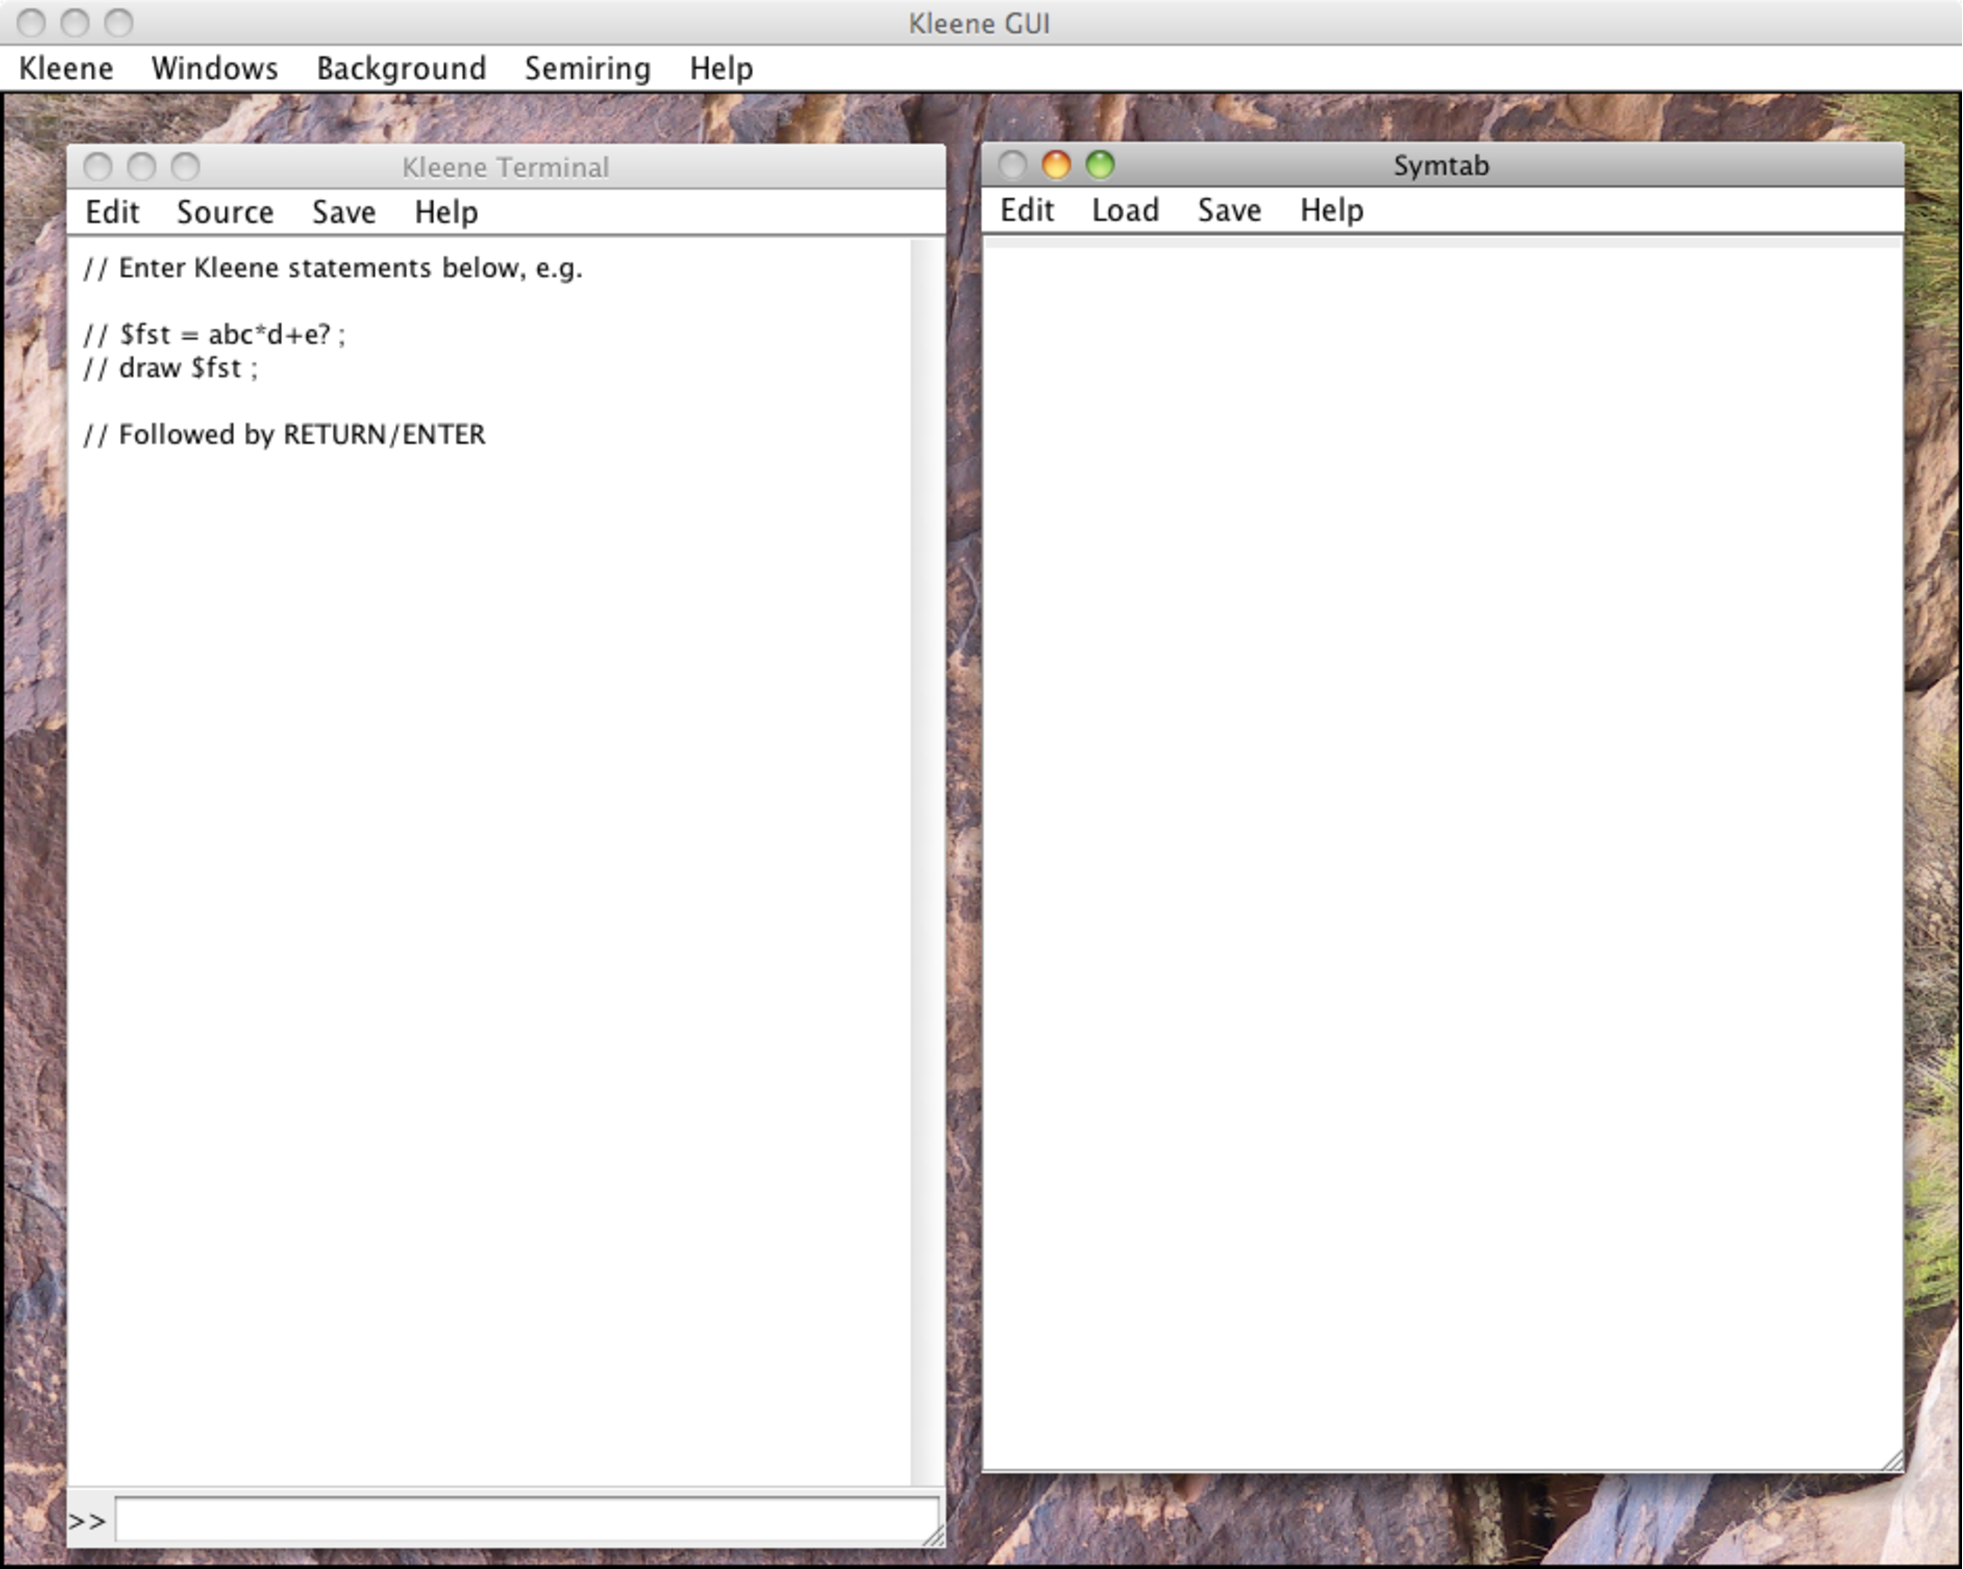
\includegraphics[width=135mm]{images/KleeneGUI.pdf}
%\includegraphics[scale=0.9]{images/<filename>.pdf}
%\includegraphics[width=60mm]{images/<filename>.pdf}
%\includegraphics[height=60mm]{images/<filename>.pdf}
\end{center}


The look-and-feel will be a little different on OS X and Linux.  The
application window, which almost fills the screen, can be minimized using
the buttons at the top.  Inside the application window, there is a
pseudo-terminal window\footnote{It is called a \emph{pseudo} terminal
because it allows you to type commands, and view responses, in a
terminal-like window, but it lacks a history memory and other useful
features of a traditional command-line terminal application.  It is hoped
that this pseudo-terminal can be improved in the future.}  on the left,
and a symbol-table window, initially empty, on the right.  At the very
bottom of the pseudo-terminal window, there is an active one-line text
field where you can enter commands to program (and learn) Kleene
interactively.  

\section{OK, What can you do in Kleene?}

\subsection{First, is it working?}

Just to make sure that Kleene is working, enter the following carefully in the bottom line of the
pseudo-terminal window:

\begin{Verbatim}
$fsm = dog | cat | bird ;
\end{Verbatim}

\noindent
Be sure to include the semicolon at the end, and press the Enter key on your keyboard to
initiate interpretation.  If everything is working, you should see an icon named
\verb!$fsm!
appear in the symbol-table window on the right.  Your statement has 
been successfully interpreted to
build a finite-state machine.  In this case, it is an \fsm{} that encodes the
language that contains just three words:  ``dog,'' ``cat'' and ``bird.''

\subsection{Visualizing Finite-State Machines}

To view the finite-state machine that you just created, you can right-click on the \verb!$fsm! icon and
select the drop-down-menu item
named \texttt{draw}.  Equivalently, you can enter 


\begin{Verbatim}
draw $fsm ;
\end{Verbatim}

\noindent
manually in the pseudo-terminal.  In fact, selecting the \texttt{draw} menu
item causes the statement \verb!draw $fsm ;! to be written in the
pseudo-terminal, and then interpreted, exactly as if you had typed it yourself.  This
behavior is designed to help you learn the scripting language.

If everything is working correctly, you should see the following \fsm{}
diagram appear on your screen.


\begin{center}
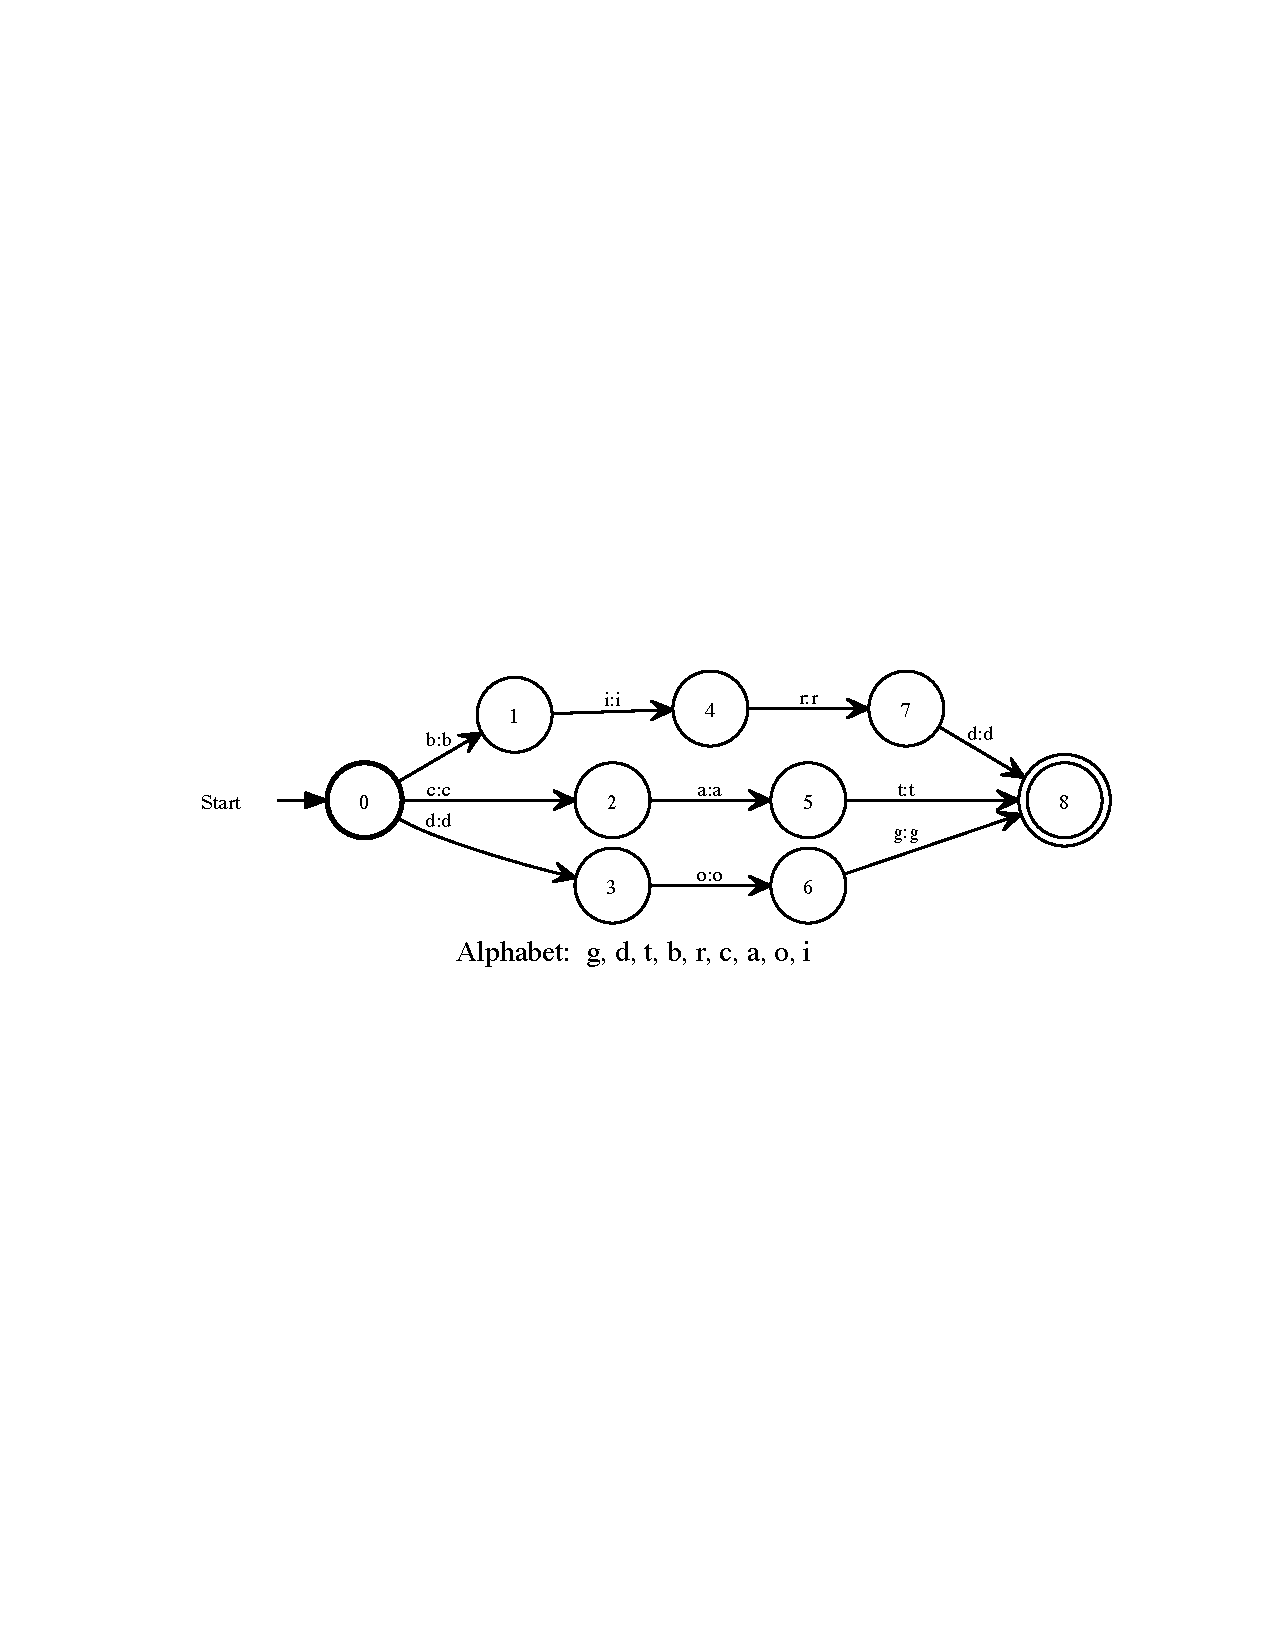
\includegraphics[width=135mm]{images/dogcatbird.pdf}
%\includegraphics[scale=0.9]{images/<filename>.pdf}
%\includegraphics[width=60mm]{images/<filename>.pdf}
%\includegraphics[height=60mm]{images/<filename>.pdf}
\end{center}


Note that the finite state machine (\init{fsm}) has a start state, represented by a bold
circle labeled ``Start,'' a single final state represented with a double circle, and
other states
represented with plain circles.  Where the \fsm{} has \texttt{n} states, they are
numbered in a dense range from \texttt{0} to \texttt{n - 1}.  The start state is
often, but not always, number \texttt{0}.   This particular \fsm{} has three \emph{paths} leading from the
start state to the final state, each path encoding one word.

Each transition or \emph{arc} leading from a state to a
state has a label like \texttt{d:d}.  The first \texttt{d} is termed the \emph{input
symbol}, and the second the \emph{output symbol}, in the OpenFst visualization of
\init{fsm}s.  Thus the compound labels are always interpreted as
\texttt{InputLabel}:\texttt{OutputLabel}.

In other traditions, \init{fsm}s are visualized a bit differently, and
the terminologies
vary, sometimes confusingly.  A label like \texttt{d:d} could be thought of as
\texttt{LeftSymbol}:\texttt{RightSymbol}.  In the Two-Level-Morphology tradition,
\fsm{}s are usually  visualized vertically, with upper-side symbols
called \emph{lexical} symbols, because they matched symbols in a lexicon, and
with lower-side symbols called \emph{surface} symbols, because they matched
symbols in surface strings: \texttt{Lexical}:\texttt{Surface}.  

The Xerox/\acro{parc} tradition also visualizes \fsm{}s vertically but
emphasizes the bi-directionality of
transducers: either side could be \emph{used} as the input side, and so the opposite
of the side currently being used as the input side is the output side.  
Abstracting away from how a
particular \fsm{} is being used, Xerox researchers often refer to
the labels as \emph{upper} and \emph{lower}:  \texttt{Upper}:\texttt{Lower}.  

Kleene is based on the OpenFst library, but with some powerful semantic features
borrowed from
the Xerox tradition.  In this book, it is sometimes important to
understand an \fsm{} in OpenFst terms, as having \texttt{Input}:\texttt{Output}
labels.  At other times, where the bi-directionality of \fsm{}s is
relevant, I will talk about \texttt{Upper}:\texttt{Lower} labels. 

The ``sides'' or ``levels'' of an \fsm{} are technically known as \emph{projections}, and we will 
refer to the input and output projections when thinking in OpenFst terms, and we will
refer to the upper and lower projections when thinking in Xerox terms.

\subsection{Compile regular expressions into \fsm{}s}

\subsubsection{Assignment Statements}

The example that we used previously for testing

\begin{Verbatim}
$fsm = dog|cat|bird ;
\end{Verbatim}

\noindent
is an assignment statement that has a variable \verb!$fsm! on the left-hand side and a
\emph{regular expression} on the right-hand side, all terminated with a semicolon.  Such
a statement can continue over multiple lines.

Many programmers will already have experience with programming languages, such as Perl,
Python and Java, that support a kind of regular expressions to
perform various useful tasks, including pattern matching and tokenization.  While these
Perl-like regular expressions are often very useful, they are not always \emph{regular}
in the mathematical sense, and so they don't have all the attractive properties of truly
regular expressions.\footnote{For a thorough presentation of ``regular'' expressions as
they appear in common programming languages and operating-system utilities, see the book \emph{Mastering Regular Expressions} by
\citet{friedl:2006}.}

In contrast to programming-language ``regular'' expressions, the regular expressions of Kleene are true regular
expressions in the sense that they always
encode \emph{regular languages} or \emph{regular relations}, and they compile into
finite-state machines (\fsm{}s).  Such regular languages/relations, and the
corresponding \fsm{}s, have mathematically clean and powerful \emph{closure properties}, meaning
that they can be combined together using various operations---including concatenation,
union and composition---and the results are still \emph{regular}.  These terms will be explained as we progress.


\subsubsection{Regular Expressions by Example}

We will look in detail at Kleene regular expressions in the next chapter.  
For now, let's look at some simple examples to get an
intuitive feel for regular expressions and the \fsm{}s corresponding to them.  One of the simplest regular
expressions consists of just a single letter, e.g. \texttt{d}.  Try entering the
following in the Kleene \acro{gui}.

\begin{Verbatim}
$fsm = d ;
draw $fsm ;
\end{Verbatim}

\noindent
The resulting \fsm{} has two states, one the start state and the other a final state,
with one arc labeled \texttt{d:d} leading from the start state to the final state.  


\begin{center}
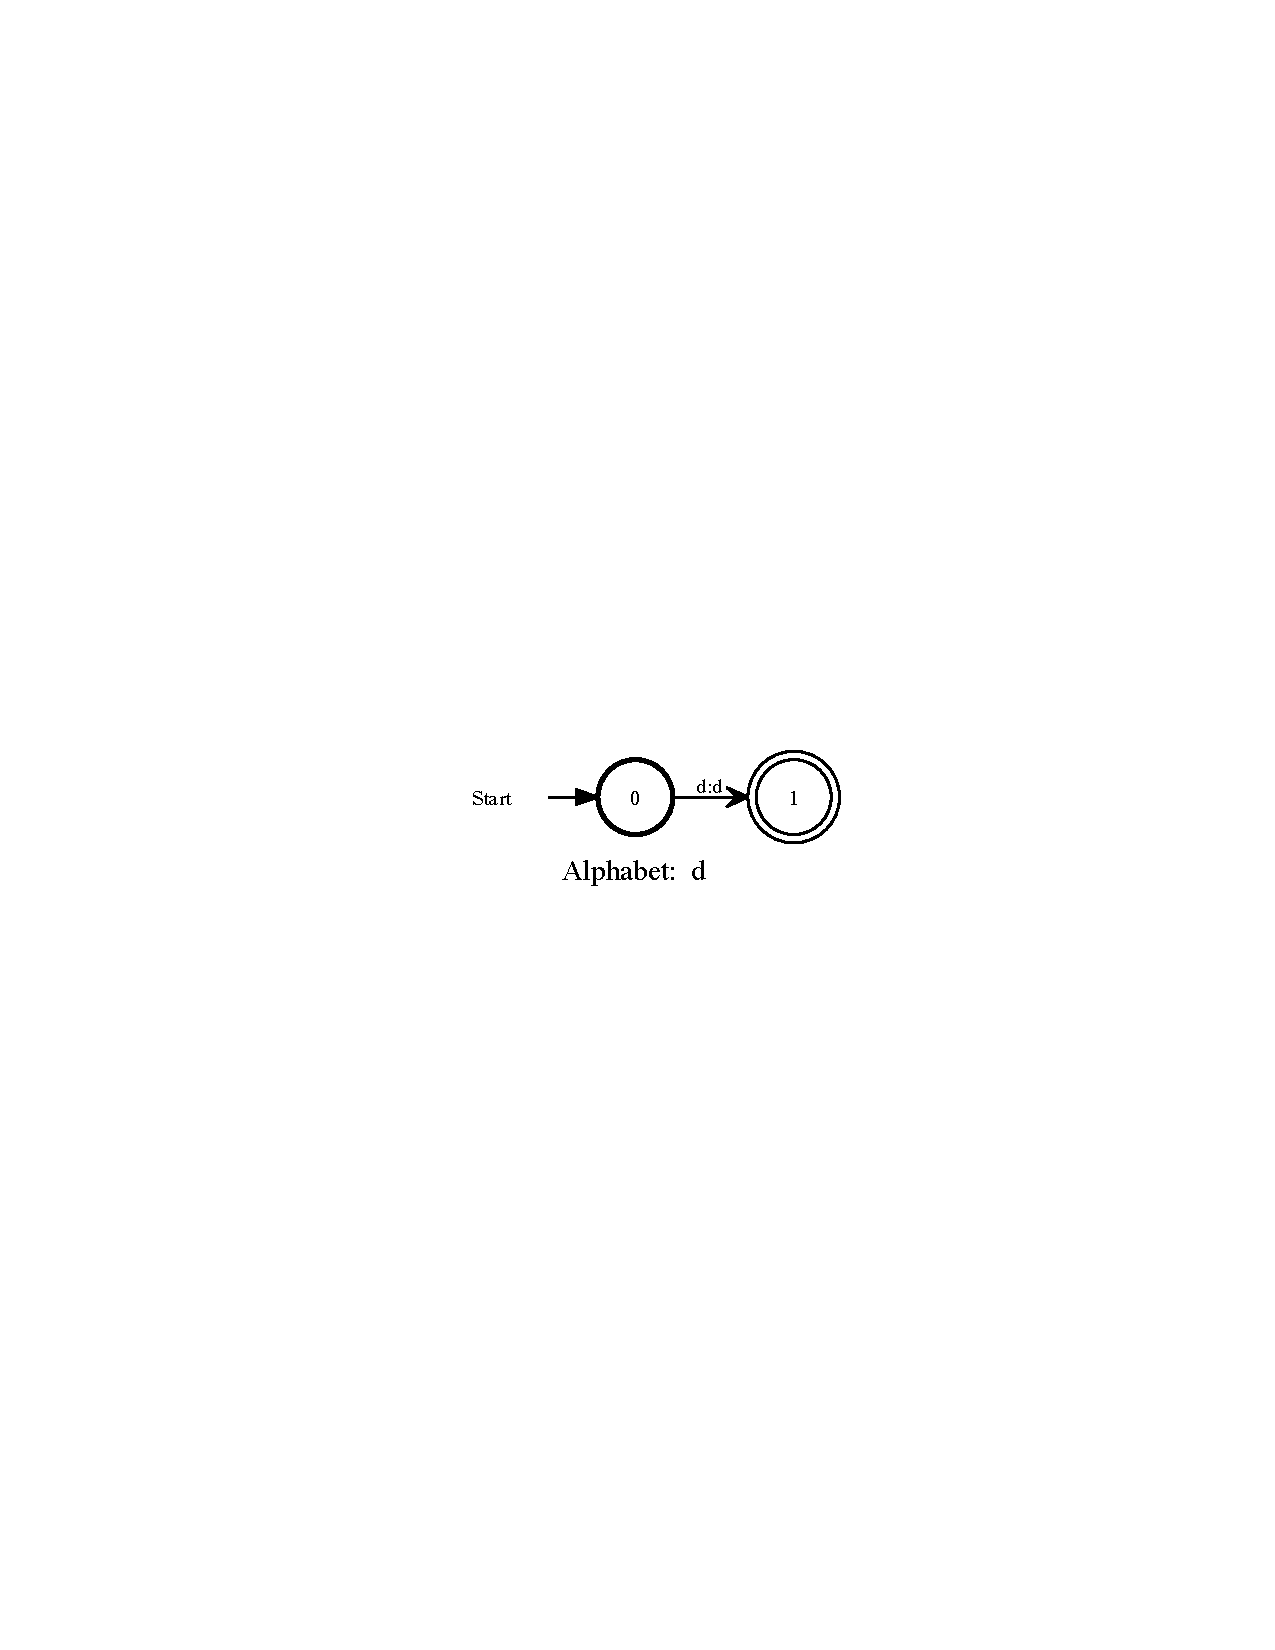
\includegraphics{images/d.pdf}
%\includegraphics[scale=0.9]{images/<filename>.pdf}
%\includegraphics[width=60mm]{images/<filename>.pdf}
%\includegraphics[height=60mm]{images/<filename>.pdf}
\end{center}

\noindent
The regular expression \texttt{d} describes the regular language consisting of just the
one string ``d.''  The \fsm{} \emph{encodes} this language, which means that if you
\emph{apply} it to the string ``d,'' it will match and \emph{accept} it, and it will reject all other
strings, including ``a,'' ``z,'' ``dog,'' ''mmmmmm,'' ``hwiughuiegw,'' etc.  An \fsm{}
can thus be used as an \emph{acceptor} that accepts all and only the strings in the
language that it encodes.

This same \fsm{} can be viewed as an \emph{identity transducer} that maps the string
``d'' to ``d,'' i.e.\@ maps ``d'' to itself.  In OpenFst, the labels on the arcs are always
two-level, \texttt{input}:\texttt{output}, or, in the Xerox visualization,
\texttt{upper}:\texttt{lower}.  An \fsm{} like that above is interpreted either as an acceptor
or as an identity transducer, depending on what is needed by an operation.

In the Kleene \acro{gui}, you can actually test an \fsm{}, to see what it accepts and rejects, by entering

\begin{Verbatim}
test $fsm ;
\end{Verbatim}

\noindent
This will bring up a test window into which you can type an input string.


\begin{center}
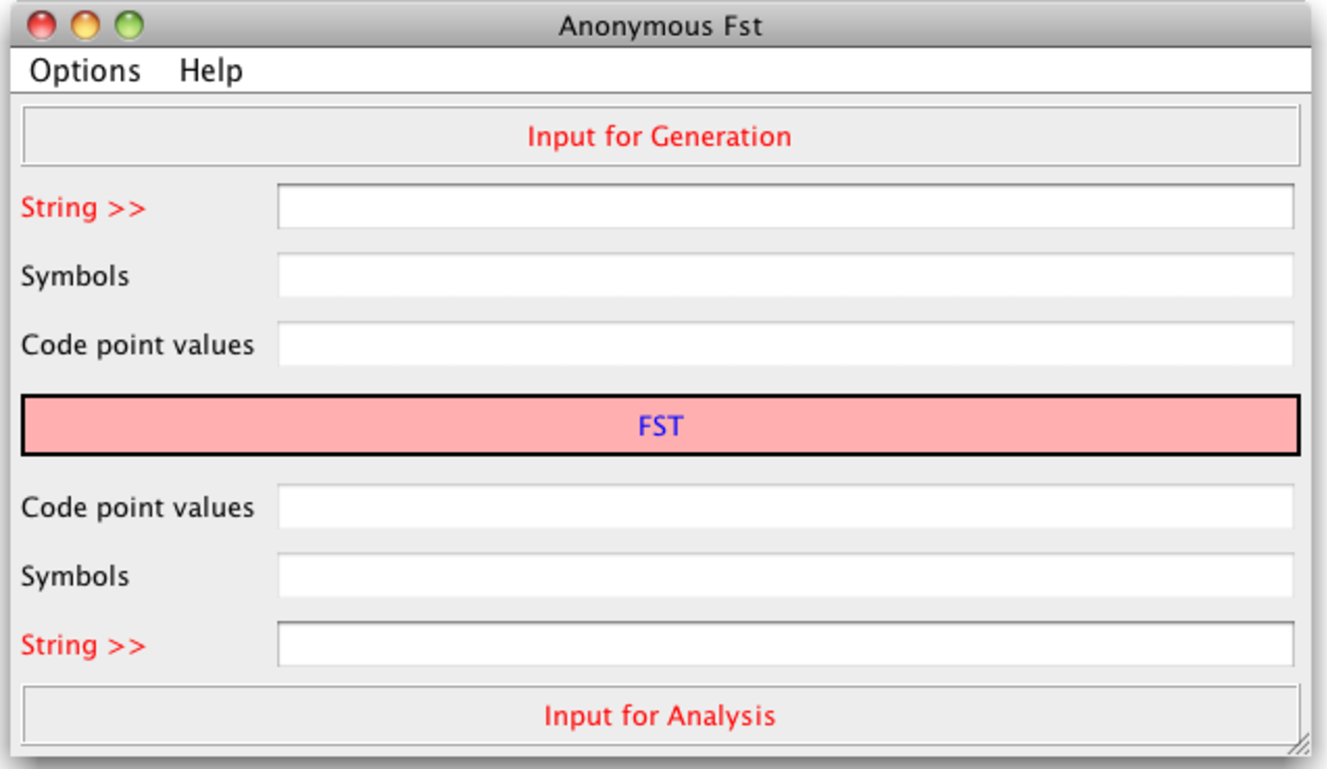
\includegraphics[width=135mm]{images/testWindow.pdf}
%\includegraphics[scale=0.9]{images/<filename>.pdf}
%\includegraphics[width=60mm]{images/<filename>.pdf}
%\includegraphics[height=60mm]{images/<filename>.pdf}
\end{center}

\noindent
The \fst{} being tested
is represented by the bar labeled ``FST'' in the center.
The test window has two string-input fields, one at the top and one at the bottom, both labeled
``String>>.''  For testing
an acceptor, it doesn't matter which field you use.  If you enter \texttt{d} in the top 
field, and then press the Enter key, the answer 


\begin{Verbatim}
d: 0.0
\end{Verbatim}

\noindent
will appear in the history part
of the pseudo-terminal window.  This indicates that the input string was accepted
by the \fsm{}.  (Don't worry now
about the ``0:0,'' which is a weight and will be explained later.)
You get the same result if you enter \texttt{d} in the
lower-side input window.  But if you enter any other string, such as ``b'' or
``ant'' or ``elephant,'' a message
indicates that the output is empty, i.e.\@ that the input string was not
accepted.

Now let's look at a slightly more complicated regular expression

\begin{Verbatim}
$fsm = dog ;
draw $fsm ;
\end{Verbatim}

\noindent
that involves the \emph{concatenation} of three characters: \texttt{d} followed by
\texttt{o} followed by \texttt{g}.   In Kleene regular expressions, there is no
explicit operator for concatenation; you just type one symbol after another---or
more generally, one operand after another---and they will be concatenated.  
The argument to the \texttt{draw} command can be
an arbitrarily complex regular expression, so one could alternatively just enter

\begin{Verbatim}
draw dog ;
\end{Verbatim}

The \fsm{} that encodes this language, consisting
of the one string ``dog,'' has four states and tree arcs.

\begin{center}
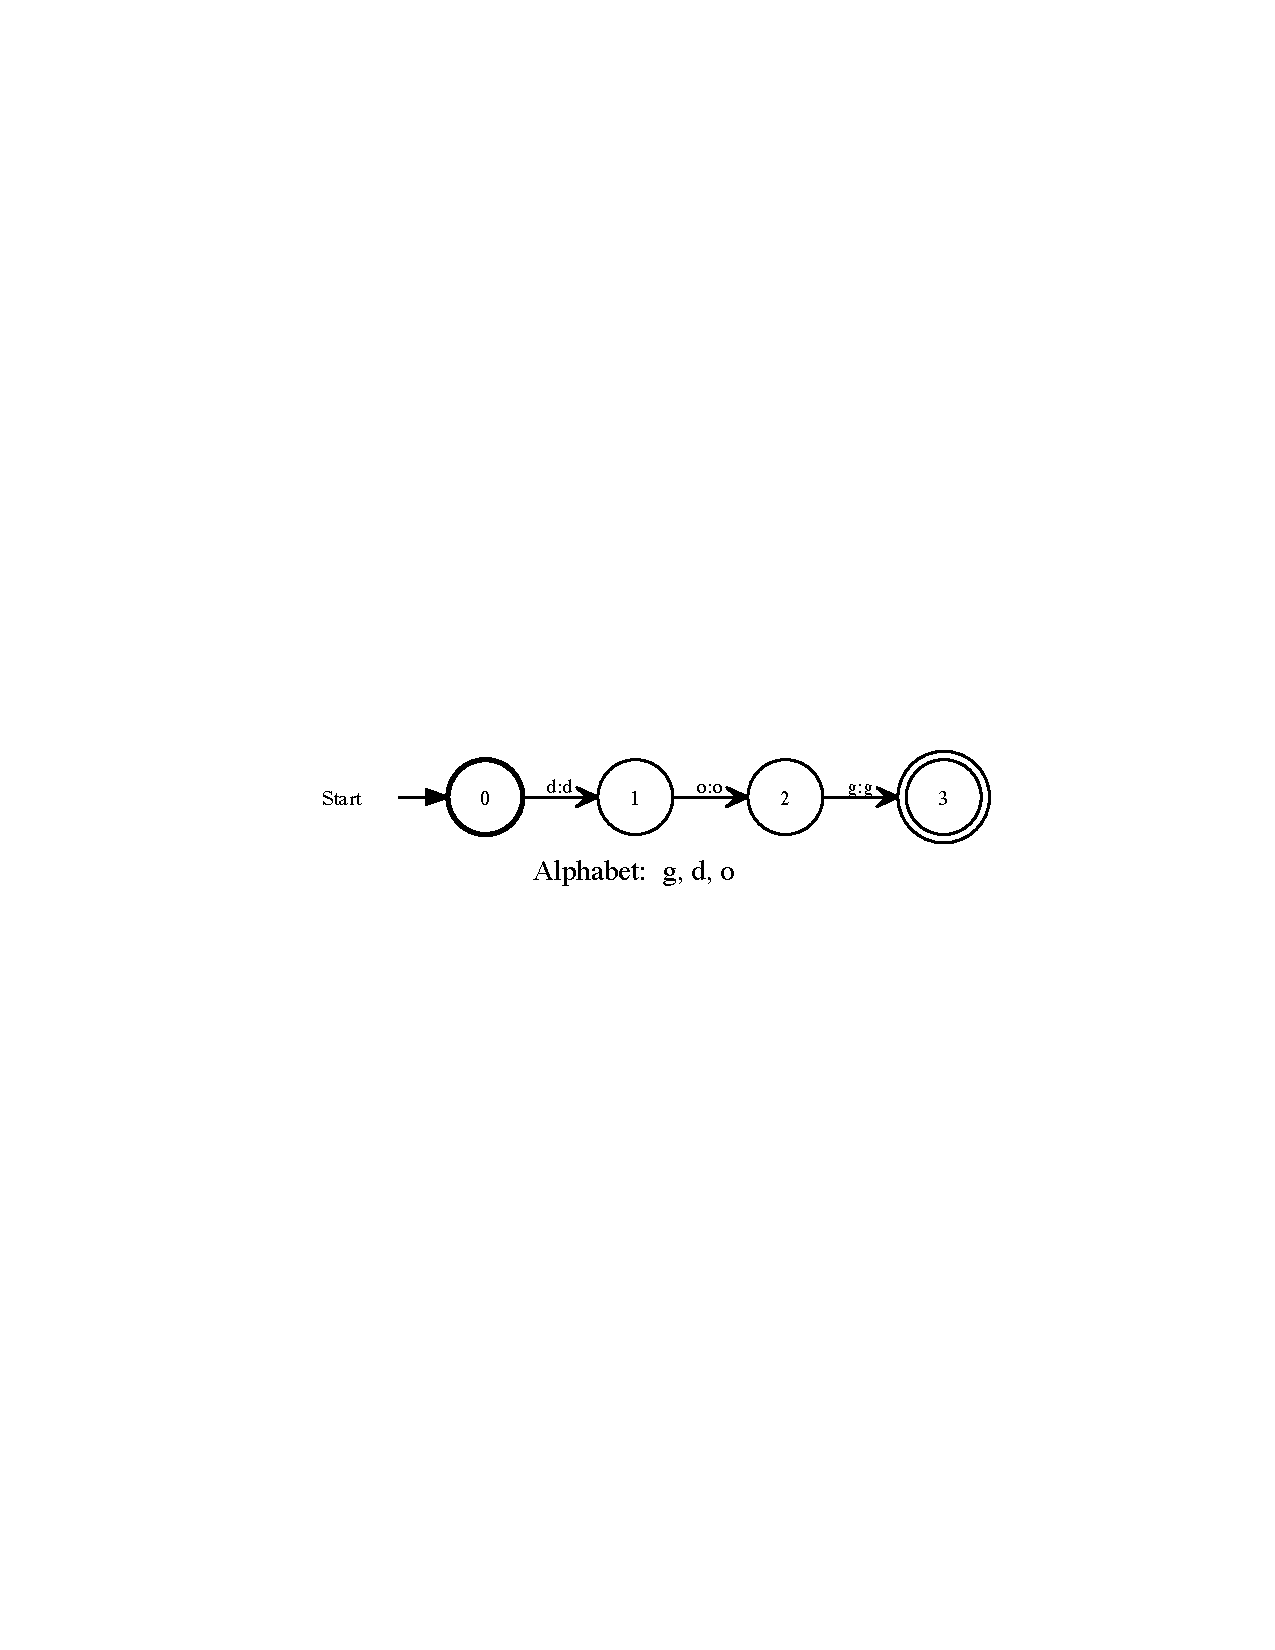
\includegraphics{images/dog.pdf}
%\includegraphics[scale=0.9]{images/<filename>.pdf}
%\includegraphics[width=60mm]{images/<filename>.pdf}
%\includegraphics[height=60mm]{images/<filename>.pdf}
\end{center}

The testing procedure that \emph{applies} this \fsm{} to the string ``dog,'' involves
first setting a match pointer to the first character \texttt{d} in the input string, 
putting the machine in
its start state, and then looking for an arc labeled \texttt{d} leading out of the
start state.  There is such an arc in this example, so the application 
\emph{consumes} the input symbol \texttt{d}, resets the match pointer to the next
symbol \texttt{o}, and resets
the machine to state 1,
which is the destination state of the arc labeled \texttt{d}.
The current
state of the machine is now state 1.  From the current state, the
process continues, matching and consuming the \texttt{o}, and putting the machine in
state two; then matching and consuming the \texttt{g}, leaving the machine in state 3.
Because state 3 is a final state (indicated by the double circle), and because the input 
string is fully consumed (no input symbols are left over), the
application is a success, and the finite-state machine matches and \emph{accepts} the input string
``dog.''  If this machine were applied to any other input string, it would fail to match, and the
string would be rejected.   

Note that a finite-state machine (\fsm{}) has a finite number of states---though there
might be hundreds of thousands or even millions of them---and there is no other memory
mechanism, such as a stack, used during application.  At any given time during
application, a finite-state machine is in exactly one of its finite number of states.
And when a machine is in a particular state, the only thing that affects its
progression
to the next state is the next input symbol; it has no stack or other memory to
influence where it goes next.

Now let's try a slightly more complicated regular expression, involving both
concatenation and union, for which the operator is the vertical bar \verb!|!. 

\begin{Verbatim}
$fsm = dog|cat|bird|horse ;
draw $fsm ;
\end{Verbatim}

\noindent
For improved readability, you can insert spaces and newlines as desired, e.g.

\begin{Verbatim}
$fsm = dog
    |  cat
    |  bird
    |  horse ;
draw $fsm ;
\end{Verbatim}

\noindent
The resulting \fsm{} encodes the language of four words---``dog,'' ``cat,'' ``bird''
and ``horse''---and clearly has four \emph{paths} leading from the start state to the
final state.


\begin{center}
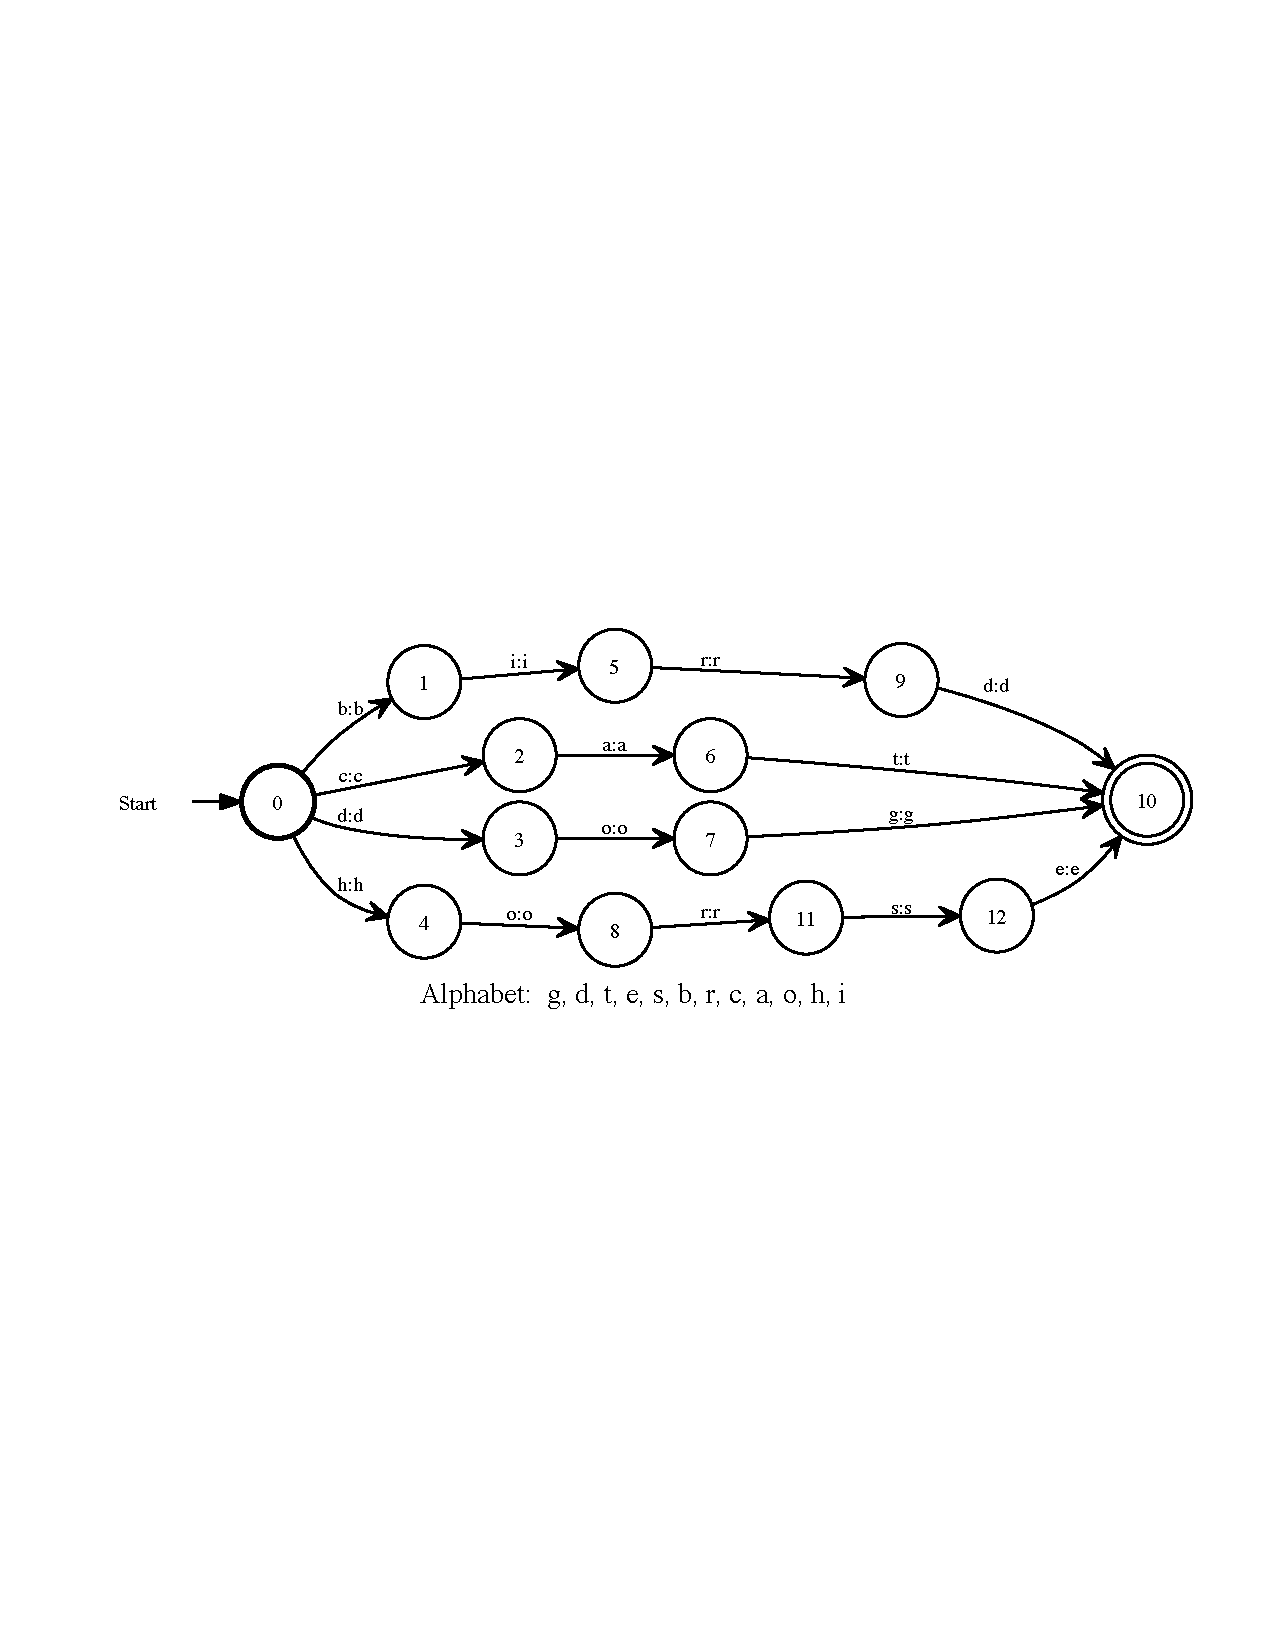
\includegraphics[width=135mm]{images/dogcatbirdhorse.pdf}
%\includegraphics[scale=0.9]{images/<filename>.pdf}
%\includegraphics[width=60mm]{images/<filename>.pdf}
%\includegraphics[height=60mm]{images/<filename>.pdf}
\end{center}

\noindent
If you test this \fsm{}, 

\begin{Verbatim}
test $fsm ;
\end{Verbatim}

\noindent
you will find that it accept the four strings, and no others.

When the \fsm{} is an acceptor, the \texttt{print} command will list the strings:

\begin{Verbatim}
print $fsm ;
// outputs:  dog cat bird horse
print Hello ;
// outputs:  Hello
print apple | orange | banana| fig | cherry ;
// outputs:  apple orange banana fig cherry
\end{Verbatim}

\noindent
Note that a language is a set of strings, and in a set, the order is
insignificant.  \fsm{}s may be constructed, and words encoded by the \fsm{}
may be printed, in orders that you didn't expect.

In general, spaces and other whitespace characters are ignored in Kleene regular
expressions unless they are explicitly literalized.  
One way to literalize spaces, and other
special characters, is to precede them with the backslash character \textbackslash.

\begin{Verbatim}
// This is a comment:
// Printing a string with a literal space
print Hello\ world ;
// outputs:  Hello world (as a single string)
\end{Verbatim}

\noindent
Another equivalent way to literalize a space is to put it inside double quotes:

\begin{Verbatim}
print Hello " " world ;
// or
print "Hello world" ;
draw "Hello world" ;
\end{Verbatim}

Kleene regular expressions, like Perl regular expressions, can also use parentheses for
grouping, a postfixed asterisk * meaning zero or more, a postfixed plus-sign +,
meaning one or more, and a postfixed question mark ? indicating that the preceding
expression is optional.  The following example encodes the words ``dog,'' ``cat'' and
``horse,'' each with an optional \texttt{s} on the end, for a total of six strings.

\begin{Verbatim}
$fsm = ( dog | cat | horse ) s? ;
print $fsm ;
// outputs:  dog dogs cat cats horse horses
\end{Verbatim}

\noindent
And this next example encodes the language of all strings that start with zero or more
\texttt{a} letters, followed by one or more \texttt{b} letters, followed by a
\texttt{c}, \texttt{d}, \texttt{e} or \texttt{f}, and ending with an optional
\texttt{g}.

\begin{Verbatim}
$fsm = a*b+(c|d|e|f)g? ;
\end{Verbatim}

\noindent
This language is infinite in size but still regular, and it is
encoded in a compact \fsm{}.


\begin{center}
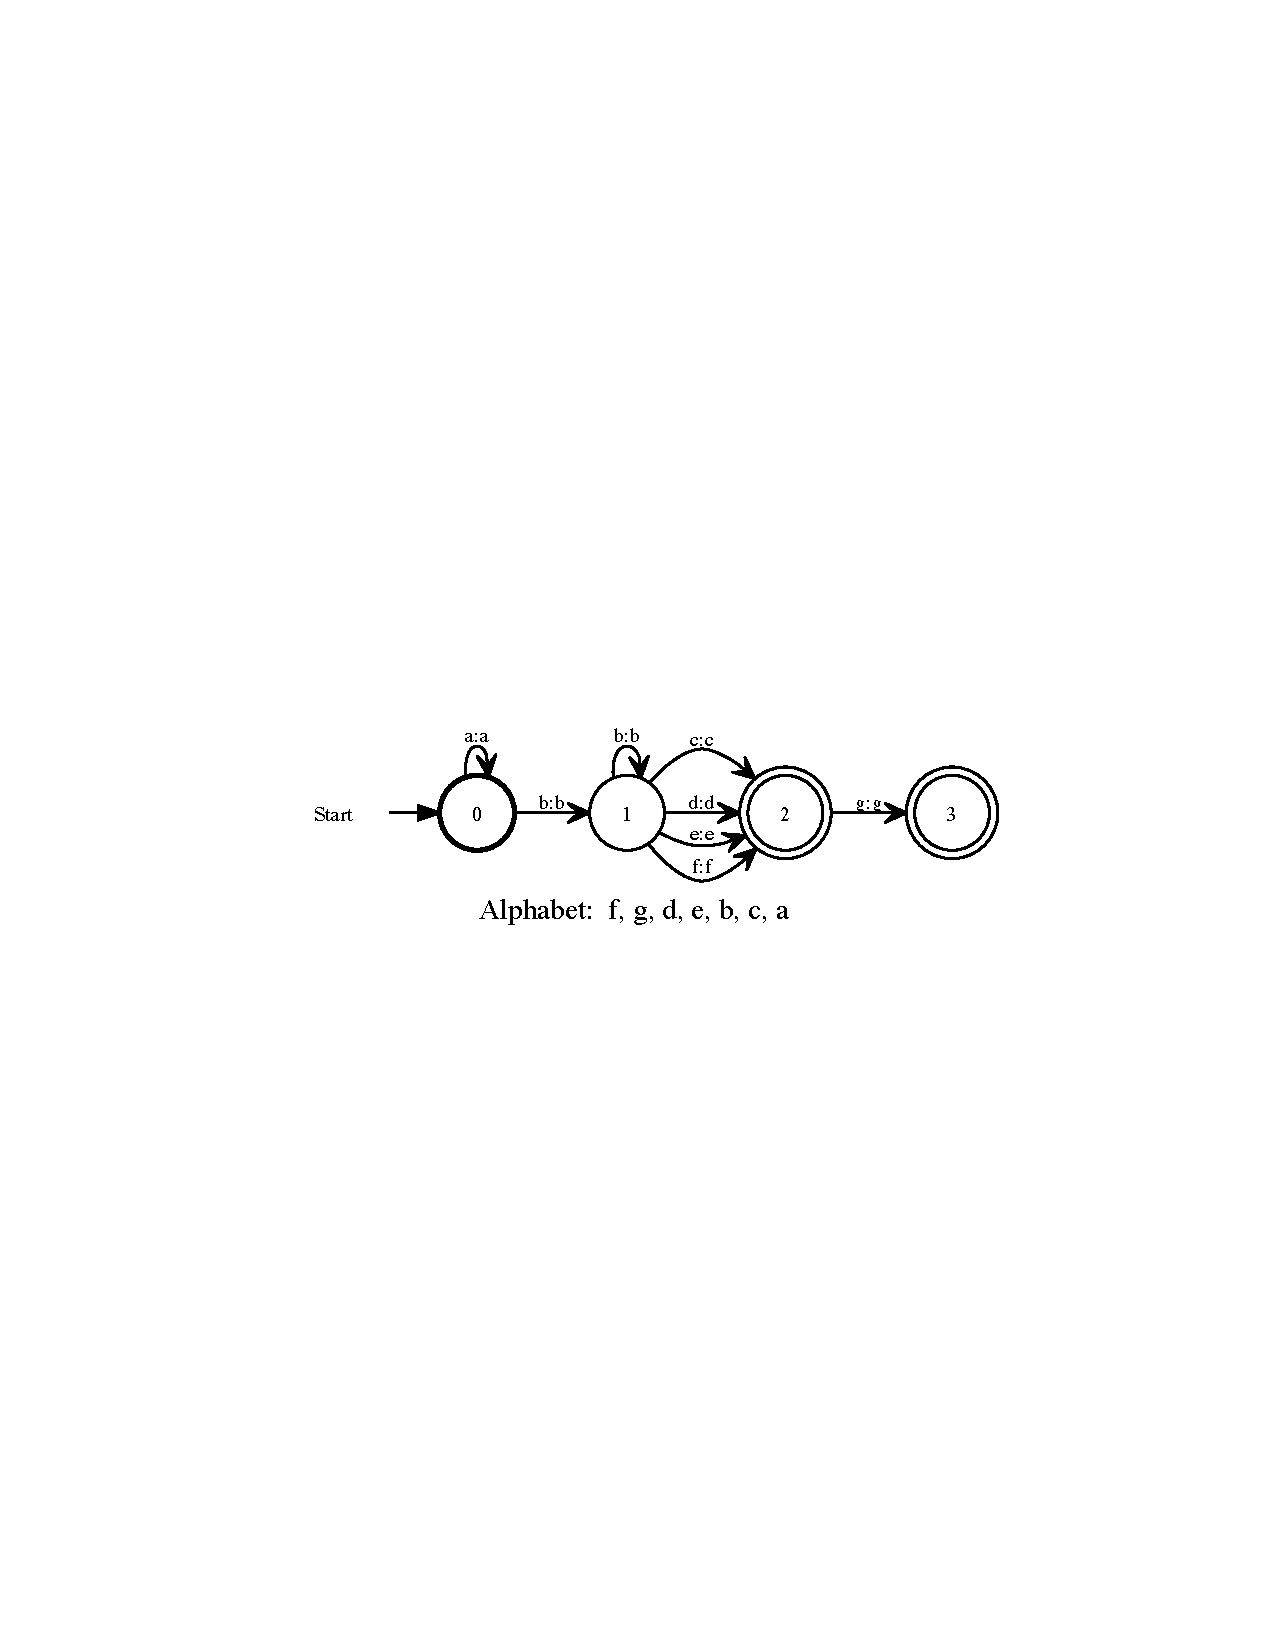
\includegraphics{images/infin.pdf}
%\includegraphics[scale=0.9]{images/<filename>.pdf}
%\includegraphics[width=60mm]{images/<filename>.pdf}
%\includegraphics[height=60mm]{images/<filename>.pdf}
\end{center}

When it becomes tedious to type long unions of symbols, e.g.
\texttt{(a|b|c|d|}\ldots{}\texttt{x|y|z)} one can
use the Perl-like square-bracketed notation for character unions: for
example, \texttt{[a-z]} encodes the union of all characters starting at
\texttt{a} and ending with \texttt{z}.  Similarly, \texttt[aeiou] denotes
the union of \texttt{a}, \texttt{e}, \texttt{i}, \texttt{o} and \texttt{u}.


\begin{Verbatim}
// Three equivalent regular expressions
$fsm1 = a*b+(c|d|e|f)g? ;
$fsm2 = a*b+[cdef]g? ;
$fsm3 = a*b+[c-f]g? ;
\end{Verbatim}

\noindent
The following example encodes the language of all strings that start with an English
alphabet letter, uppercase or lowercase, and then continues with zero or more alphabetic letters or digits:

\begin{Verbatim}
$fsm = [A-Za-z][A-Za-z0-9]* ;
\end{Verbatim}

\noindent
The resulting \fsm{} will accept strings like ``Apple,'' ``a27,'' ``dOg,''
``z3b4n6'' and
``d2T456m7'' while rejecting strings such as ``4abc'' and ``26.''

Regular languages can be subtracted from each other:

\begin{Verbatim}
$lang = (dog | cat | elephant | apple | orange) - 
           (banana | apple | orange) ;
print $lang ;
// outputs: dog cat elephant
\end{Verbatim}

\noindent
Here, the resulting \fsm{} encodes the language consisting of the strings ``dog,'' ``cat'' and ``elephant.''
It is \emph{not} necessary to put spaces around the vertical-bar operator |.
As already stated, white space is ignored in Kleene regular expressions
unless it is explicitly literalized.

Regular languages can also be intersected, resulting in a new language
containing all and only the strings they have in common.
The operator for intersection is \&.

\begin{Verbatim}
$commonAnimals = 
   (dog | cat | elephant | whale | ant | bird | reindeer) & 
   ( cat | horse | reindeer | snail | whale )
print $animals ;
// outputs: cat whale reindeer
\end{Verbatim}

The . (dot) represents \emph{any} symbol, so the \fsm{} resulting from the
assignment statement

\begin{Verbatim}
$fsm = p . t ;
\end{Verbatim}

\noindent
accepts words including ``pat,'' ``pet,'' ``pit,'' ``pot'',
``put,'' ``pbt,'' ``ppt,'' etc.  And because . really 
represents any symbol, the expression
\verb!.*! represents the Universal Language, the language that contains all possible
strings of any character, of any length, including the empty (zero-length) string.

\begin{Verbatim}
$UnivLang = .* ;
\end{Verbatim}

\noindent
Note that in Kleene, as in the Xerox Finite State Toolkit, is it not necessary
for the programmer to declare the alphabet being used.  The . really represents any possible symbol.

The Empty Language is the language that contains no strings at all, not even the empty
string.  There are an infinite number of ways to denote the Empty Language, including

\begin{Verbatim}
$EmptyLang = .* - .* ;   // Universal Language minus itself
$EmptyLang = dog - dog ; // one-string language minus itself
\end{Verbatim}

\noindent
and

\begin{Verbatim}
$EmptyLang = ~.* ;
\end{Verbatim}

\noindent
where \~{} is the \emph{complement} operator, returning the language of all possible
strings, i.e.\@ the Universal Language, except
(i.e.\@ minus) the strings in the language it applies to.  Thus \texttt{\~{}.*} is
equivalent to \texttt{.* - .*}, the Universal Language minus itself.

The empty string is the string of zero length, containing no symbols at all.  It can be
notated in Kleene as \verb!""!.  The Empty String Language, not to be confused with the Empty
Language, is the language that contains exactly one string, the empty string.

\begin{Verbatim}
$EmptyStringLang = "" ;
\end{Verbatim}

\subsection{Optimization of \fsm{}s}

When \fsm{}s are built in Kleene, they are automatically \emph{optimized}, which involves a
combination of determinization, minimization and epsilon-removal.  The epsilon, which can be
denoted as \verb!""! in regular expressions, is the empty
(zero-length) string, and epsilon-removal involves the
elimination of all arcs that have [eps]:[eps] labels.  Thus the assignment


\begin{Verbatim}
$fsm = a "" c ;
\end{Verbatim}

\noindent
creates a network that initially looks like 

\begin{center}
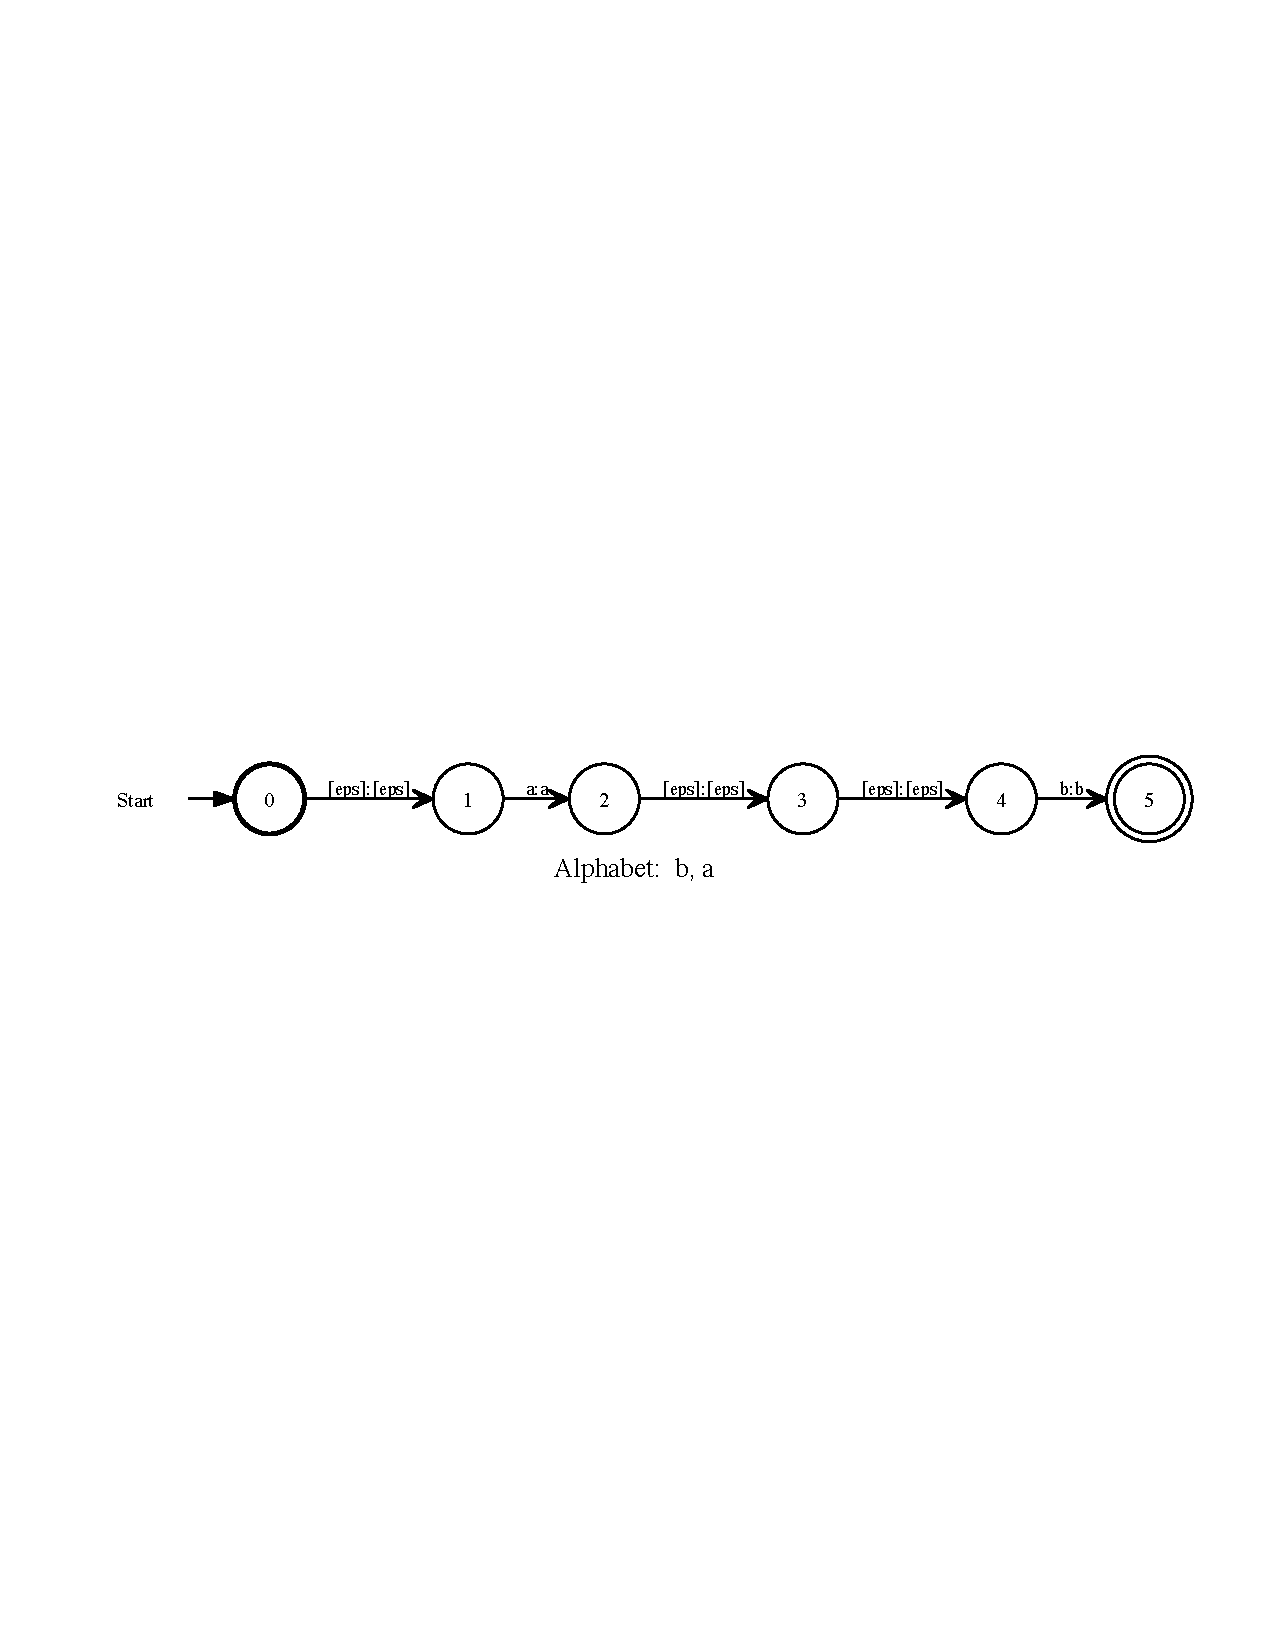
\includegraphics[width=135mm]{images/aEpsb.pdf}
%\includegraphics[scale=0.9]{images/<filename>.pdf}
%\includegraphics[width=60mm]{images/<filename>.pdf}
%\includegraphics[height=60mm]{images/<filename>.pdf}
\end{center}

\noindent
including the epsilon indicated by the regular expression, plus two other epsilons
introduced by the concatenation algorithm.  By default, however, the \fsm{}
is automatically epsilon-removed to produce the equivalent but more compact result

\begin{center}
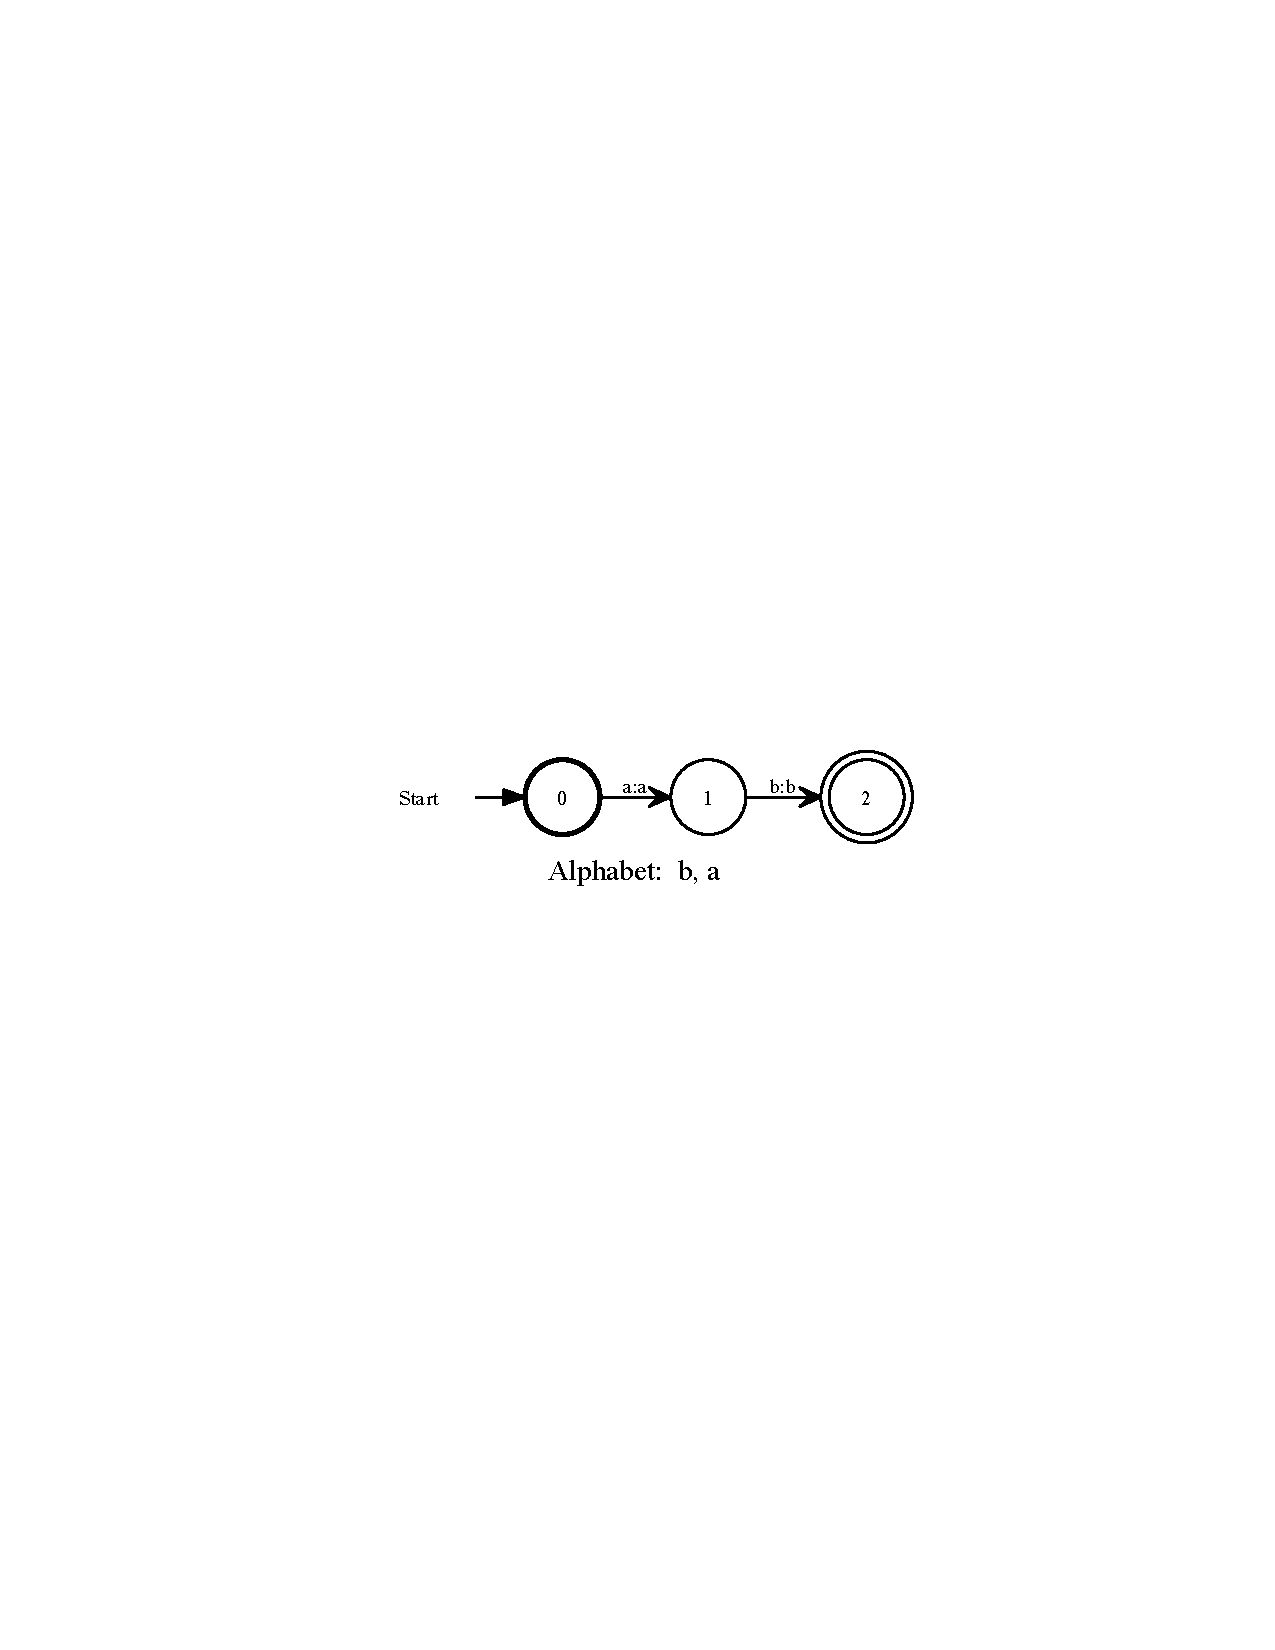
\includegraphics{images/aEpsbOptimized.pdf}
%\includegraphics[scale=0.9]{images/<filename>.pdf}
%\includegraphics[width=60mm]{images/<filename>.pdf}
%\includegraphics[height=60mm]{images/<filename>.pdf}
\end{center}

Consider also the following example, which has multiple words that start
with the same symbol(s) and multiple words that end with the same
symbol(s).


\begin{Verbatim}
$foo = rat | bat | rabbit | bird | cod ;
\end{Verbatim}

\noindent
The raw, unoptimized \fsm{} looks like this, including a number of
epsilon arcs:


\begin{center}
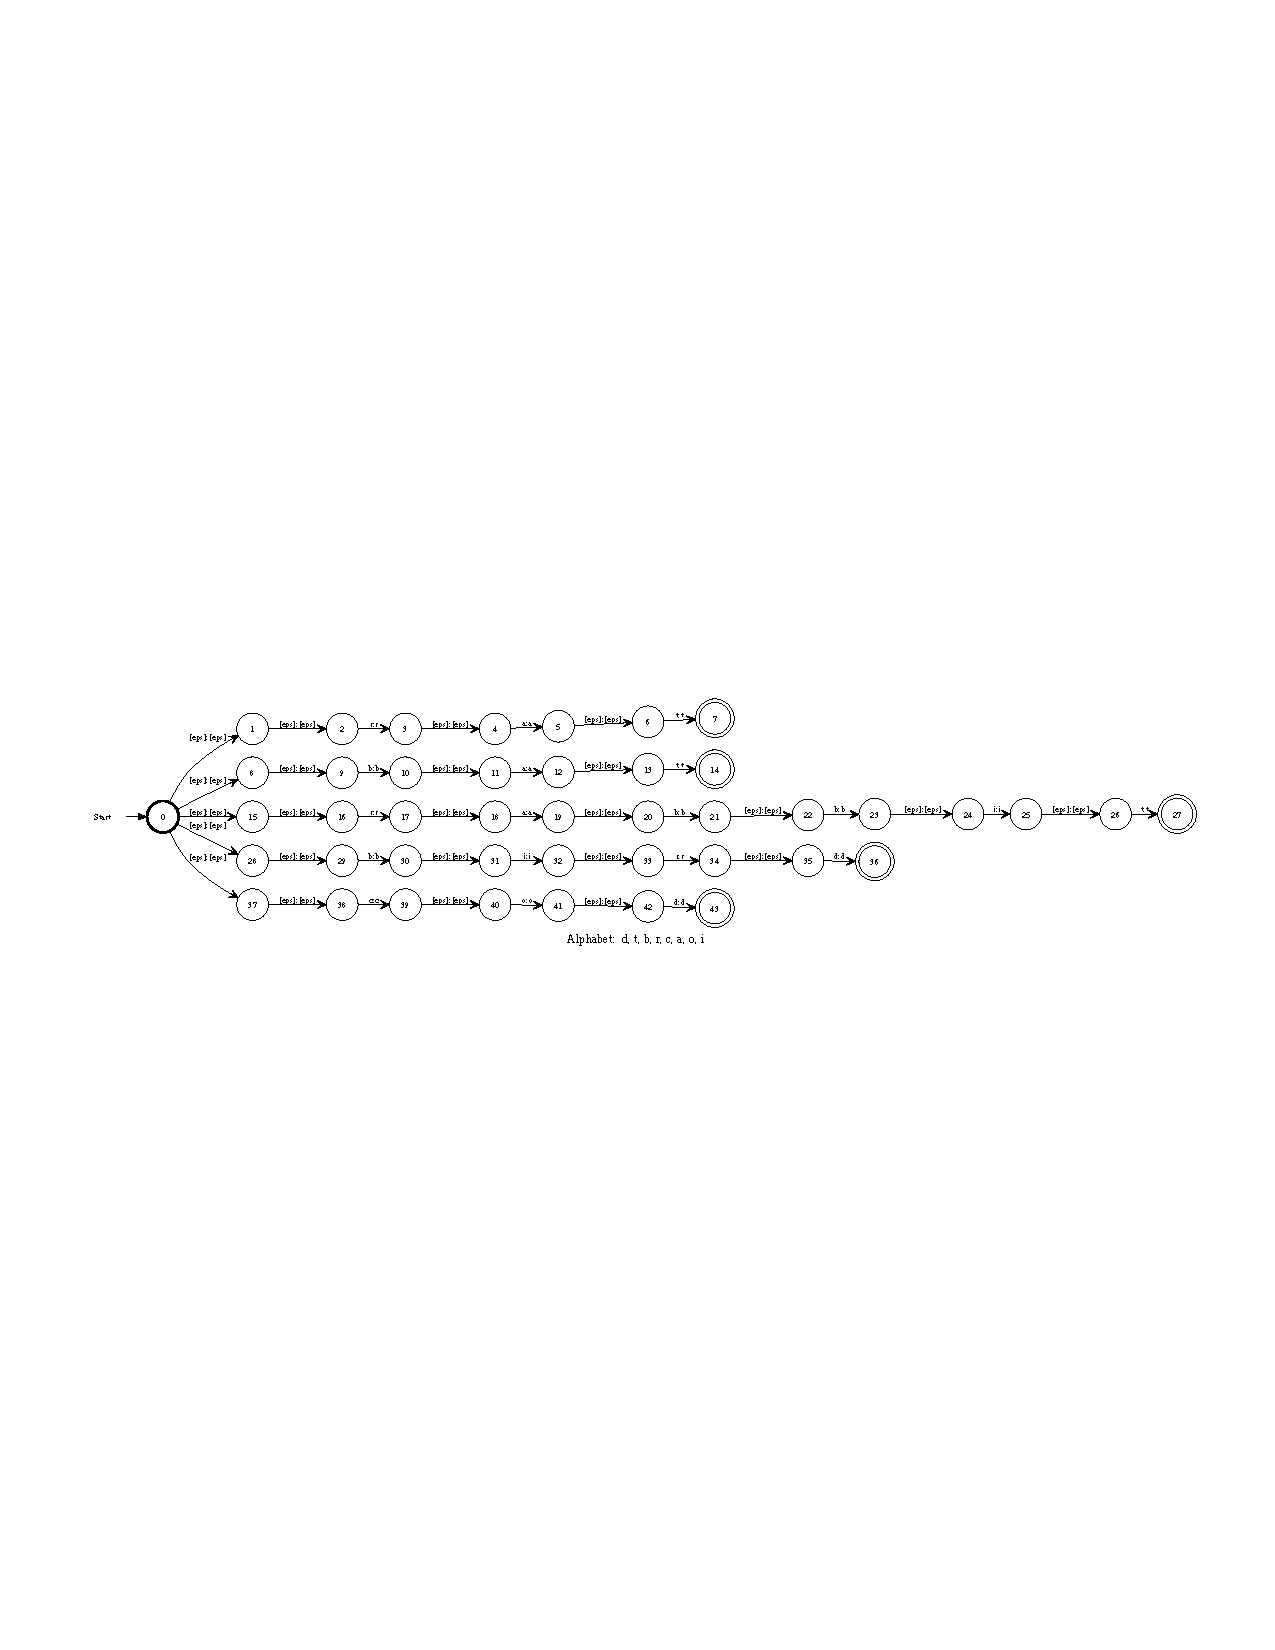
\includegraphics[width=135mm]{images/unoptimized.pdf}
%\includegraphics[scale=0.9]{images/<filename>.pdf}
%\includegraphics[width=60mm]{images/<filename>.pdf}
%\includegraphics[height=60mm]{images/<filename>.pdf}
\end{center}

\noindent
This machine accurately encodes the five-word language, but in a less than
optimal way.
Just by running epsilon-removal, the \fsm{} is considerably simplified,
resulting in the following machine:


\begin{center}
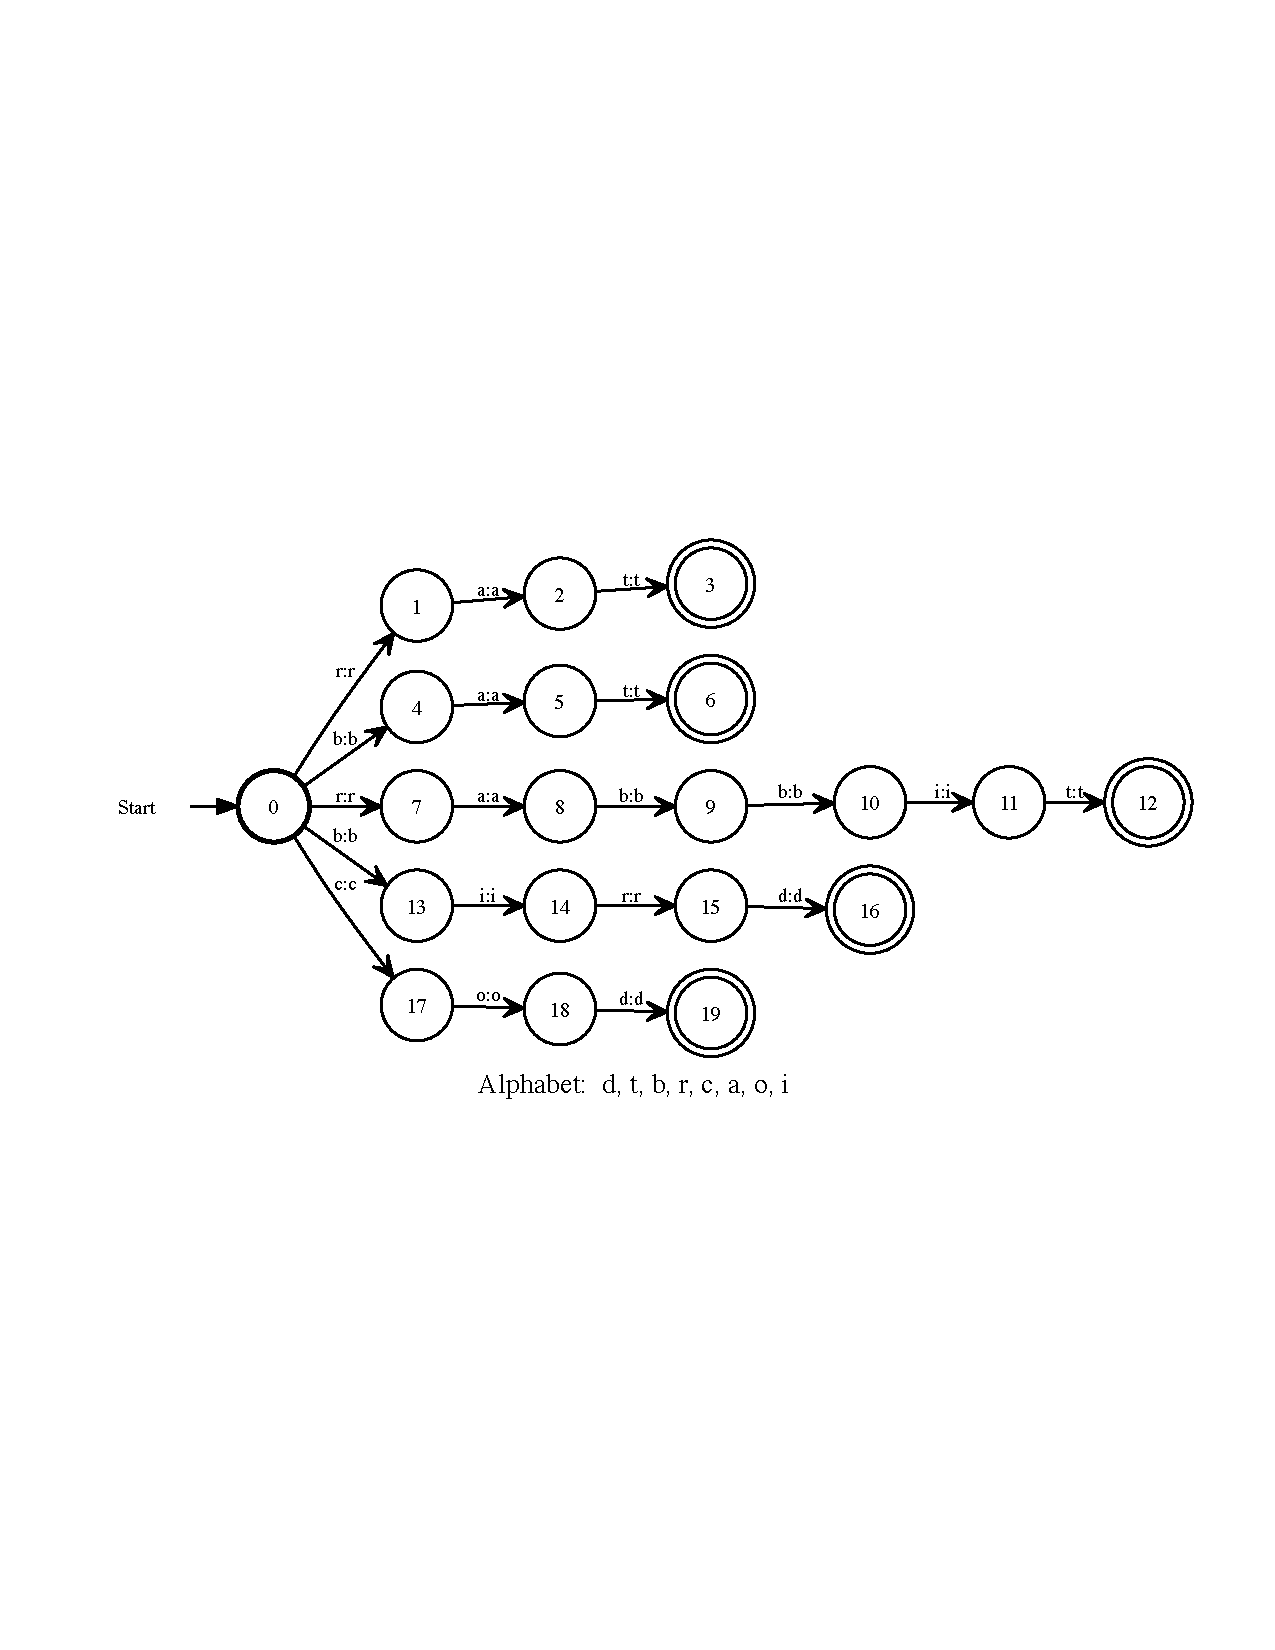
\includegraphics[width=135mm]{images/epsremoved.pdf}
%\includegraphics[scale=0.9]{images/<filename>.pdf}
%\includegraphics[width=60mm]{images/<filename>.pdf}
%\includegraphics[height=60mm]{images/<filename>.pdf}
\end{center}

\noindent
At this point, note that if you apply the machine to the input string
``rat,'' its operation is going to be \emph{non-determnistic}.  Starting in
the machine's start state, and placing the match pointer at the first input symbol
\texttt{r}, there are in fact two arcs labeled \texttt{r} exiting the start state, 
and both of these arcs will need to be
explored.  Of course, only one of them will result in a successful match, 
but time will be wasted
exploring the wrong \texttt{r}-labeled arc. 

The solution to the non-determinism problem is to \emph{determinize} the
\fsm{}, resulting in the following modified machine


\begin{center}
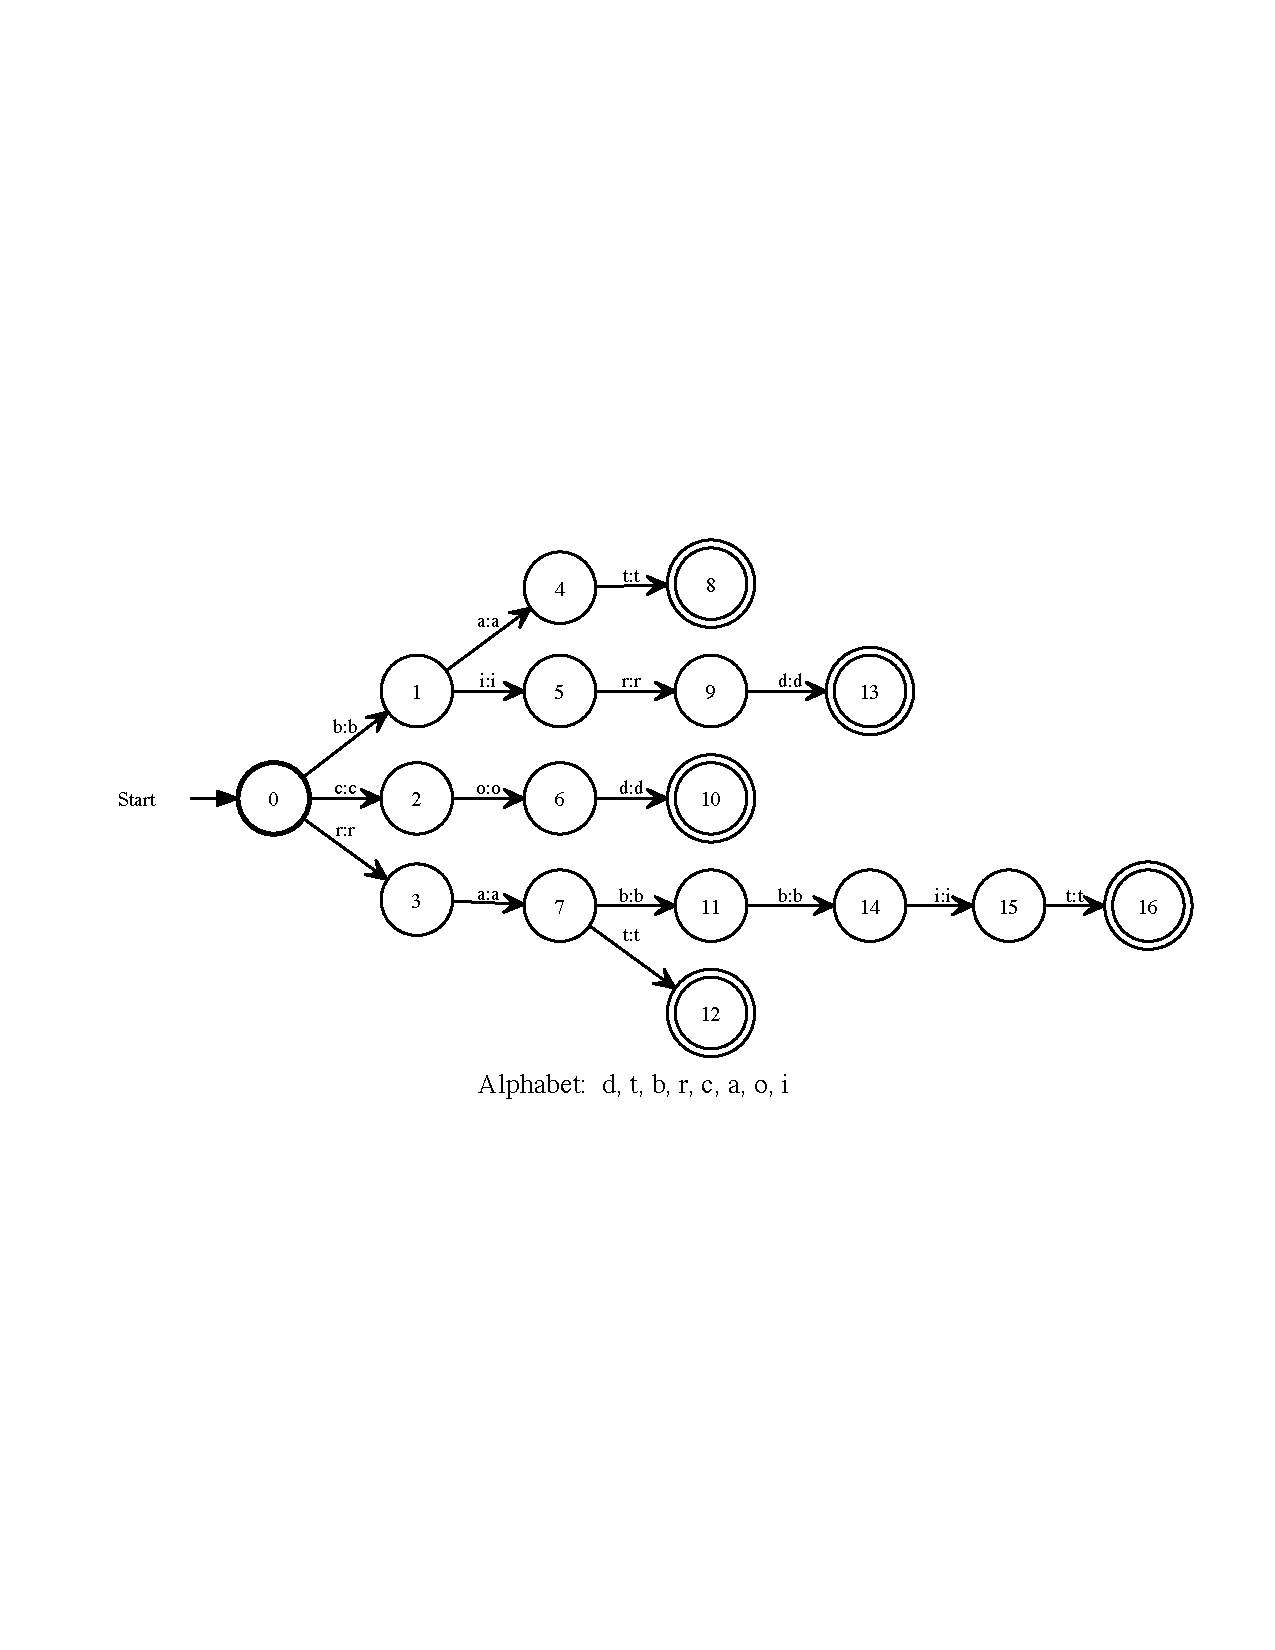
\includegraphics[width=135mm]{images/determinized.pdf}
%\includegraphics[scale=0.9]{images/<filename>.pdf}
%\includegraphics[width=60mm]{images/<filename>.pdf}
%\includegraphics[height=60mm]{images/<filename>.pdf}
\end{center}

\noindent
Note that the paths for the words ``rat'' and ''rabbit,'' which both start
with the prefix ``ra,'' now share the states and arcs for recognizing that
prefix.  When the determinized machine is applied to ``rat'' or ``rabbit,'' the
application algorithm no longer wastes time exploring the wrong path.  Note
also that the \texttt{b} prefix shared by ``bat'' and ``bird'' is also
represented in the machine by shared states and arcs.

At this point, we have a deterministic machine that can be applied to input
strings with maximum efficiency, but note that the machine itself is bigger
than it really needs to be.  In particular, note that ``rat,'' ``bat'' and
``rabbit'' all end with the same \texttt{t} suffix, but the \fsm{}
represents them with separate states and arcs.  The solution to this problem
is to \emph{minimize} the machine, resulting in this final optimal machine:


\begin{center}
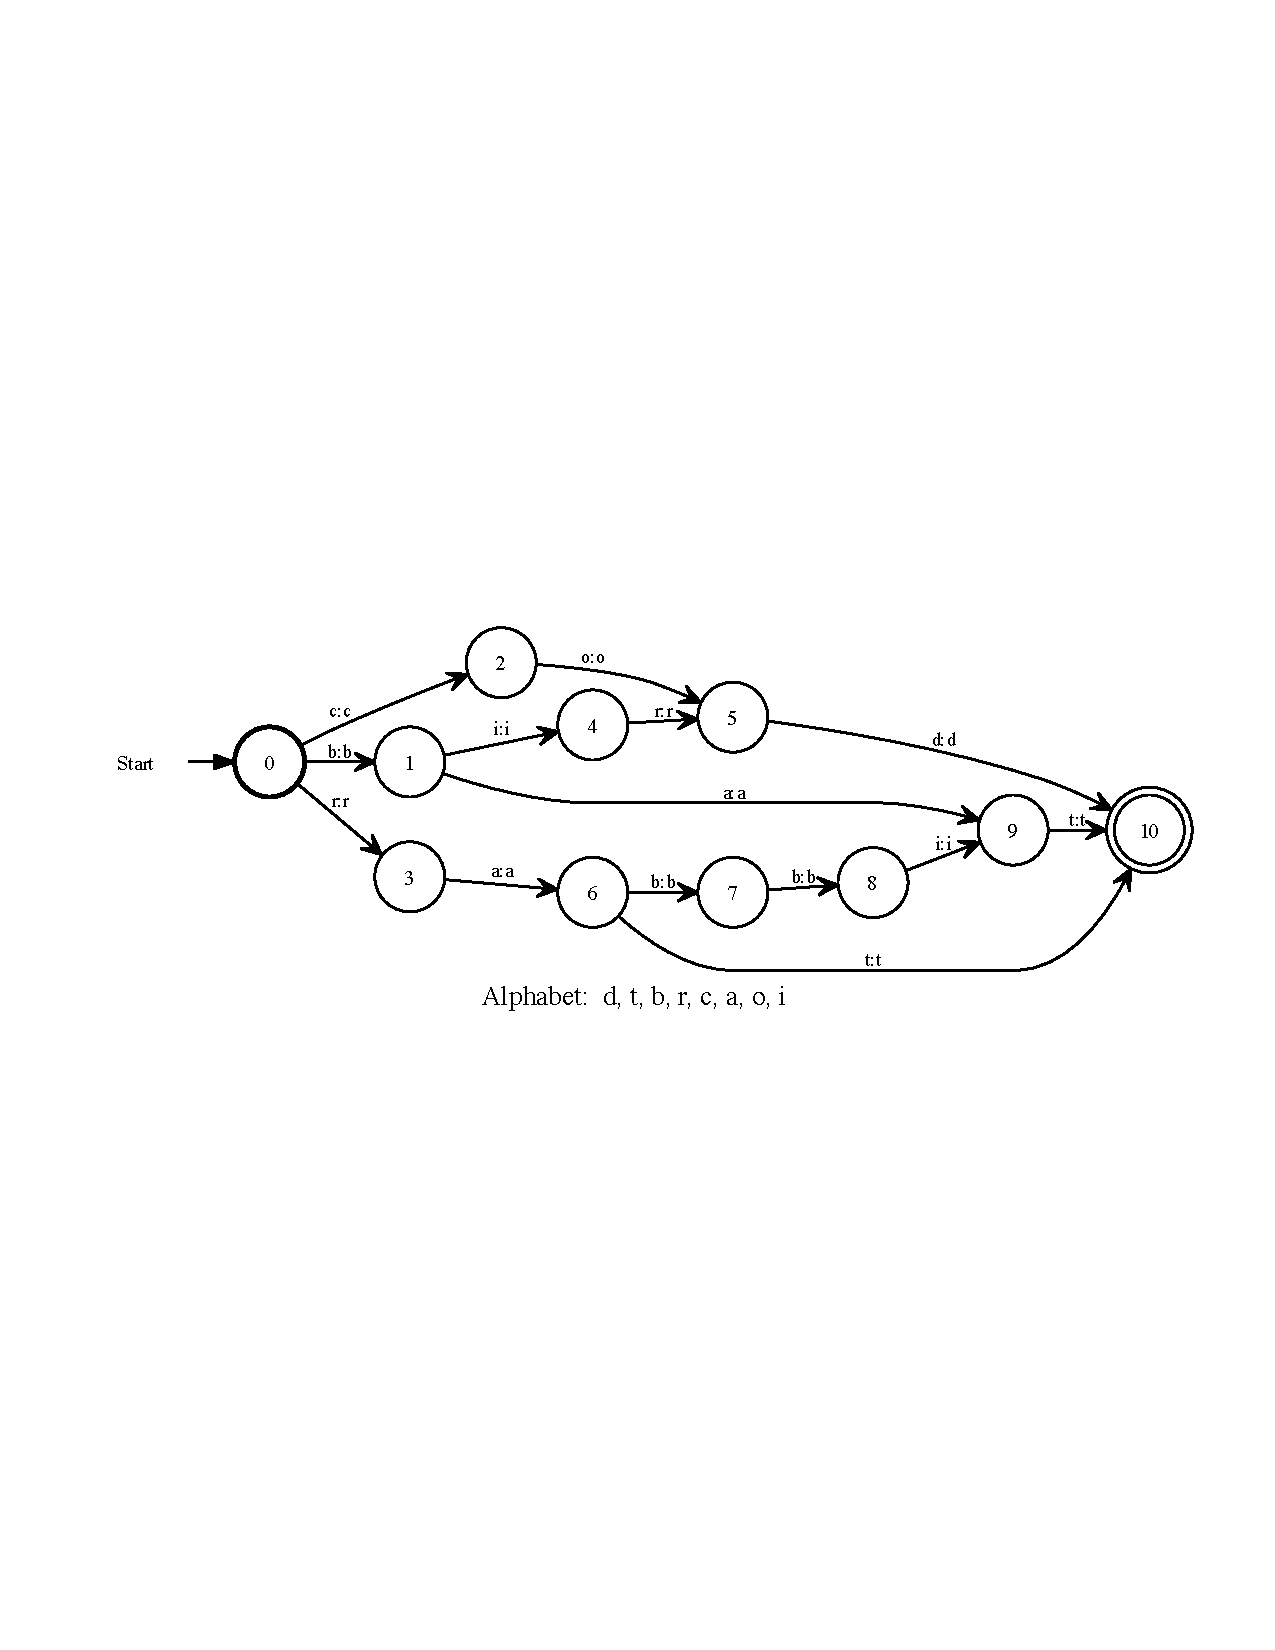
\includegraphics[width=135mm]{images/minimized.pdf}
%\includegraphics[scale=0.9]{images/<filename>.pdf}
%\includegraphics[width=60mm]{images/<filename>.pdf}
%\includegraphics[height=60mm]{images/<filename>.pdf}
\end{center}

As you will recall, we started with the superficially simple regular
expression


\begin{Verbatim}
$foo = rat|bat|rabbit|bird|cod ;
\end{Verbatim}

\noindent
At each stage shown, the \fsm{} encoded the same language of five words, but
as we epsilon-removed, determinized and minimized the machine, it became
both more efficient to apply, and smaller in its storage requirements.  In
real-life applications, where \fsm{}s can encode languages of millions of words, and the
machines can easily contain tens of thousands of states and arcs, and
runtime performance is critical, the
processes of epsilon-removal, determinization and minimization---known
collectively as \emph{optimization}---are vital.  Luckily, Kleene
automatically optimizes all \fsm{}s by default, and the average Kleene
programmer never has to worry about it.\footnote{Expert users may occasionally
want to turn off one or more of the optimization processes, and Kleene provides
a way to do this.  See Appendix \ref{app:optimize}.} 

\subsection{Using Defined Variables}

Once a variable has been bound to an \fsm{} value, it can be used in subsequent regular
expressions, e.g.

\begin{Verbatim}
$fsm1 = dog | cat | elephant ;
$fsm2 = horse | pig | sheep ;
$fsm = $fsm1 | $fsm2 ;
print $fsm ;
// outputs: dog cat elephant horse pig sheep
\end{Verbatim}


\subsection{Characters}

\subsubsection{Unicode}

Kleene supports the Unicode character set, 
which current contains over 100,000 defined characters and has a capacity
to encode over 1 million characters.  Programmers are encouraged to edit their Kleene scripts
directly in Unicode using their favorite Unicode-capable text editors, though Kleene 
can read and process scripts written in all common character sets.  

The Kleene \gui{} is written using the Java Swing library; its text widgets are
automatically Unicode-capable, and you can use standard Java input methods to facilitate
typing in exotic characters.  In some cases, it may be convenient to designate Unicode
characters by their code point value.  Unicode characters in the Basic Multilingual Plane
can all be encoded using four hexadecimal digits, and in Kleene regular expressions they
can be designated as the \acro{ascii} sequence \verb!\uHHHH!, where \texttt{H} is in the
set [0-9a-fA-F].\footnote{That is, each \texttt{H} can be a digit from 0 to 9 or a letter
from \texttt{A} to \texttt{F}, in either uppercase or lowercase.}  The following two
examples are equivalent,


\begin{Verbatim}
$fsm1 = a b c α β γ ;
$fsm2 = a b c \u03b1 \u03b2 \u03b3 ;
\end{Verbatim}

\noindent
because 03b1 (hexadecimal) is the code point value of the Greek alpha, 03b2 is the beta,
and 03b3 is the gamma.  Both expressions result in an \fsm{} that looks like


\begin{center}
\includegraphics[width=135mm]{images/alphabetagamma.pdf}
%\includegraphics[scale=0.9]{images/<filename>.pdf}
%\includegraphics[width=60mm]{images/<filename>.pdf}
%\includegraphics[height=60mm]{images/<filename>.pdf}
\end{center}

\noindent
In OpenFst (and Kleene) \fsm{}s, the labels on arcs are in fact integers,
and in Kleene these integers are Unicode code point values.  Where possible,
the code point values are displayed by the \texttt{draw} facility as
letters.  The Graphiviz \texttt{dot}
facility, which is used to display the \fsm{}s, has limitations in displaying characters
like α, β and γ, so they are displayed in hexadecimal.  

Kleene can also handle Unicode supplementary characters, and they can be entered as the
\acro{ascii} sequence
\verb!\uHHHHHHHH!, that is, \verb!\u! followed by exactly eight hexadecimal digits.  The following
example contains the first three characters in the Deseret Alphabet, which is encoded in
the supplementary area.


\begin{Verbatim}
$fsm = \U00010400 \U00010401 \U00010402 ;
draw $fsm ;
\end{Verbatim}

\noindent
This results in the following \fsm


\begin{center}
\includegraphics[width=135mm]{images/desalph.pdf}
%\includegraphics[scale=0.9]{images/<filename>.pdf}
%\includegraphics[width=60mm]{images/<filename>.pdf}
%\includegraphics[height=60mm]{images/<filename>.pdf}
\end{center}

\noindent
which has a single supplementary code point value on each arc.\footnote{However, if the
characters are entered in a Swing text widget using the Java CodePoint Input Method, each
character is somehow divided into the two \init{bmp} surrogate characters used to encode
the single supplementary character in the UTF-16 encoding.  This behavior needs to be
reviewed in the context of Kleene.}



\subsubsection{Multi-character Symbols}

In addition to Unicode characters, it is often useful to have user-defined symbols that
have multi-character names, often called ``multi-character symbols.''  For example, you can
define [Noun], [Verb], [Adj], [Adv], [Sing], [Plur], etc.\@ as symbols that suggest
linguistic categories or features.  In another notational tradition, these might be spelled +Noun,
+Verb, +Adj, etc.  In Kleene syntax, you simply surround a string of characters in single quotes
to indicate that they are to be treated as a single multi-character symbol.


\begin{Verbatim}
$fsm = a b '[Noun]' ;
\end{Verbatim}

\noindent
The single quotes delimit the name of the symbol but are not actually part of the symbol
name.  Each multi-character symbol is also stored as an integer label on an arc in the result
\fsm{}, and the integer is taken from a Unicode Private Use Area (\init{pua}).

In general it is recommended that multi-character symbol names include at least
one punctuation character to help human beings distinguish them from sequences of
alphabetical characters.  There is nothing to prevent you from using a
multi-character symbol like \texttt{noun}, by putting \verb!'noun'! in a regular
expression,


\begin{Verbatim}
// a multi-character symbol without punctuation, NOT recommended
$myfsm = 'noun' ;
print $myfsm ;
// outputs: noun

// a concatenation of four symbols
$yourfsm = noun ;
// outputs: noun
\end{Verbatim}

\noindent
but the printed output \texttt{noun}, being a single multi-character symbol,
is humanly indistinguishable from the printed word ``noun''
that is a concatenation of four separate symbols.  In practice, the use of
multi-characters symbols like \verb'noun' leads to much confusion and is
strongly discouraged.  

\subsubsection{Characters in Variable Names}

\fsm{} variable names in Kleene start with a dollar sign, a letter, and then any number of
letters and digits.


\begin{Verbatim}
$fsm = a b c ;
$fsm1 = x y z ;
$q7 = r s t ;
\end{Verbatim}

\noindent
The letters after the dollar sign can include any letters in the Unicode \init{bmp} (Basic
Multilingual Plane).\footnote{Because of limitations in JavaCC and Java itself, variable
names cannot contain supplementary characters.}  The following two assignments are equivalent 


\begin{Verbatim}
$αβ = a b ;
$\u03b1\u03b2 = a b ;
\end{Verbatim}

Kleene supports Unicode to the extent that Java does, which is pretty well but not
perfectly.  Users can write their scripts using the International Phonetic Alphabet, Greek,
Cyrillic, Arabic, etc.\@ without ever needed to resort to clumsy transliterations.
Whether the Kleene \gui{} can actually display a character depends on the fonts installed in
your Java installation.

\subsection{Regular Languages and Regular Relations}

\subsubsection{Regular Languages and Acceptors}

In formal language theory, a language is a set of strings.  A regular language, where
\emph{regular} is a technical term, is formally defined as a language that can be defined
using only concatenation, union and the Kleene-closure\footnote{The Kleene-closure is named
after mathematician Steven Cole Kleene, who invented it.  The Kleene programming language
is named after the same man.} operator *, which indicates zero or
more repetitions.  Any finite (i.e.\@ not infinite) language is a regular language.  Some infinite languages,
such as \verb!b*!, which is the language of all strings that contain zero or more
\texttt{b} letters, are also regular.  Some infinite languages are not regular
and so cannot be encoded in an \fsm{}; we cannot handle such languages in Kleene.

A regular language can be encoded as an \fsm{} (Finite-State Machine) called an
\emph{acceptor}.  An \fsm{} has a finite number of states, one of which is designated as the
start state, and zero or more of which are final.  An \fsm{} can also contain zero or
more labeled directed arcs that lead from a state to a state.

When an acceptor is applied to an input string, it will either accept it or reject it.  It
will accept all and only the strings in the regular language that it encodes.

In classic visualizations of acceptors, they have only a single label on
each arc.  In OpenFst, and therefore in Kleene, all arc labels have two labels, an input
label and an output label: \verb!i:o!.  By convention in OpenFst, an \fsm{} is an acceptor,
or can be interpreted as an acceptor,
if and only if all the labels have the same symbol as both the input and the output.

Regular languages, and the acceptors that encode them, have some very interesting and
useful
mathematical properties, known as closure properties.  For example, regular languages are
\emph{closed} under the union operation because if you union two regular languages together, the
result is also a regular language.  Regular languages and the acceptors that
encode them are closed under the following
operations:

\vspace{4mm}

\begin{tabular}{|l|l|}
\hline
Concatenation 	& A B \\
\hline
Union         	& A | B \\
\hline
Iteration	  	& A*\\
\hline
Subtraction		& A - B\\
\hline
Intersection	& A \& B\\
\hline
Complementation		& \~{}A\\
\hline
\end{tabular}

\subsubsection{Regular Relations and Transducers}

Whereas a regular \emph{language} is a set of strings, a regular \emph{relation}
is a set of
\emph{ordered pairs}
of strings.  For example, (dog, dogs), (cat, cats), (elephant, elephants), (woman, women)
and (deer, deer)
are ordered pairs of words that, in English, have a singular noun as the first word, and its plural
as the second word.  A set of such pairs, denoted in set theory (not Kleene syntax) as \{ (dog, dogs), (cat, cats), (elephant,
elephants), (woman, women), (deer, deer) \}, is a regular relation.  All finite relations are
regular relations.  Some infinite relations are also regular.

A regular relation can be encoded as an \fsm{} called a \emph{transducer}.  Theoretically,
regular relations and finite-state transducers can have any number of levels, known as
\emph{projections}, but OpenFst and most practical computer implementations have been limited to two.
A finite-state transducer (\fst{}) has a finite number of states, one of which is
designated as the start state, and zero or more of which are final.  An \fst{} can also
contain zero of more labeled directed arcs that lead from a state to a state.  Each label
consists of two parts, an input label and an output label, notated  \verb!i:o!.  The input
and output labels of an arc can be different, or the same.

In Kleene syntax, a label with \texttt{a} on the input side and \texttt{b} on the output
side is denoted \texttt{a:b}.  The statement


\begin{Verbatim}
$fsm = a:b ;
\end{Verbatim}

\noindent
results in the \fst{}


\begin{center}
\includegraphics{images/aoverb.pdf}
%\includegraphics[scale=0.9]{images/<filename>.pdf}
%\includegraphics[width=60mm]{images/<filename>.pdf}
%\includegraphics[height=60mm]{images/<filename>.pdf}
\end{center}


\noindent
More generally, : is the \emph{cross-product} operator that takes two operands that must
both denote regular languages (not regular relations).  It creates a regular relation with the
left operand as the input projection, and the right operand as the output projection.
Often the cross-product operator is used to map
individual strings, as in this example.


\begin{Verbatim}
$fsm = (dog):(dogs) | (cat):(cats) | (elephant):(elephants) |
       (woman):(women) | (deer):(deer) |
       (formula):(formulas) | (formula):(formulae) ;
\end{Verbatim}


More generally, the operands of the cross-product operator : can denote arbitrarily complex regular languages, 
and every string in the input language is related to every string of the
output language, and vice-versa.  Consider, for example,

\begin{Verbatim}
$foo = (dog|cat|rat):(animal|mammal) ;
\end{Verbatim}

\noindent
where the input (upper-side) language consists of the strings ``dog,'' ``cat'' and ``rat,'' and the output (lower-side)
language consists of the strings ``animal'' and ``mammal.''  The cross-product is an \fst{} that
relates ``dog'' in the input language to both ``animal'' and ''mammal'' in the output
language.  And similarly for ``cat'' and ``rat.''  The resulting relation
contains the six ordered pairs (dog, animal), (dog, mammal), (cat, animal), (cat,
mammal), (rat, animal) and (rat, mammal).  Note that a relation is a set of ordered string
pairs, and the order of the string pairs is not significant.

\subsubsection{Applying Transducers}

In the OpenFst visualization, an \fst{} is \emph{applied} to an input string by
matching the symbols of the input string against a sequence of \emph{input symbols}.  If the input string matches successfully
and completely against a sequence of input symbols, on a \emph{path} leading from the start state,
arc-by-arc to a final state, 
the output is a string consisting of the sequence of \emph{output symbols} from the same path 
in the \fst{}.  

The output string can be different from the input string, and thus
the \fst{} can \emph{transduce} or \emph{map} from one kind of string to another kind of string.  To return to the
previous noun example, if an ordered pair (dog, dogs) is interpreted as (\emph{inputString},
\emph{outputString}),
then the \fst{} that encodes the regular relation { (dog, dogs), (cat, cats), (elephant,
elephants), (woman, women), (deer, deer)} would provide a transduction or \emph{mapping}
from singular nouns like ``dog,'' ``cat'' and ``woman'' to their plural forms ``dogs,''
``cats'' and ``women,'' respectively.  Looked at in the other direction,
the same \fst{} provides a mapping from plural forms to their
corresponding singular forms.

Try building and testing the following example in the Kleene \gui{}:


\begin{Verbatim}
$numberMapper = (dog):(dogs) | (cat):(cats) | 
      (elephant):(elephants) | (woman):(women) | (deer):(deer) |
      (formula):(formulas) | (formula):(formulae) |
      (cherub):(cherubim) | (man):(men) | (knife):(knives) ;
test $numberMapper ;
\end{Verbatim}

\noindent
Enter a singular noun like ``dog'' in the upper-side input field, and the output
will be the plural form ``dogs.''  Enter ``formula'' in the upper-side input
field, and the output will be the two plural forms:  ``formulas'' and
``formulae.''  


An \fsm{} encoding an acceptor can also be interpreted and used as an \emph{identity transducer}
that maps each of the words in the language to itself.

An \fst{} that encodes a relation is \emph{functional} if each input string has exactly one
output string.  Very commonly when modeling natural languages, an \fst{} can map one input
string to multiple output strings, reflecting ambiguity. 

A regular relation is a relation between two regular languages, one of which is, in the
OpenFst tradition, termed the
\emph{input projection} and the other the \emph{output projection}.  In all cases, every
string in the input language/projection is related to at least one
string in the output language/projection, and each string in the output language/projection is related to at
least one string in the input language/projection.

In the Xerox
visualization of \fst{}s, which emphasizes the bi-directionality of \fst{s}, the projections
are called \emph{upper} and \emph{lower} rather than \emph{input} and \emph{output}.  
What OpenFst calls normal application, matching the symbols
of an input string against ``input'' symbols on a path, outputting the corresponding
``output'' symbols, Xerox calls \emph{generation} or ``application in a downward
direction,'' matching the symbols of the input string against upper-side labels, and
outputting strings of lower-side labels.  Xerox
researchers also talk about \emph{analysis} or ``application in an upward direction,'' matching the symbols of
the input string against lower-side symbols, and outputting strings of upper-side symbols.  

The following transducer, which includes multi-character symbols,
models the formation of regular English plurals more elegantly, and illustrates the Xerox
visualization.

\begin{Verbatim}
// a set of noun roots
$nroot = dog|cat|bird|horse|worm ;
$ncat = '[Noun]':"" ; // [Noun] tag on the upper side,
                      // the empty string on the lower side
$num = '[Sg]':"" | '[Pl]':s	; 
// [Sg] on the upper side, 
//   and empty string on the lower.
// [Pl] on the upper side, 
//   and s on the lower

// now just concatenate the three FSMs
$nouns = $nroot $ncat $num ;

test $nouns ; // and launch the test window
\end{Verbatim}

\noindent
The resulting \fst{} looks like this:

\begin{center}
\includegraphics[width=135mm]{images/simplenounsgpl.pdf}
%\includegraphics[scale=0.9]{images/<filename>.pdf}
%\includegraphics[width=60mm]{images/<filename>.pdf}
%\includegraphics[height=60mm]{images/<filename>.pdf}
\end{center}


\noindent
showing that strings like ``dog[Noun][Sg]'' and ``cat[Noun][Pl]'' are in the upper-side
language, while their related strings like ``dog'' and ``cats'' are in the lower-side language. 
The \texttt[eps] character in the diagram represents the empty-string language, called the
\emph{epsilon} by convention.
When you \texttt{test} the network and enter \texttt{cat[Noun][Pl]} in the \emph{upper}-side
entry field, the output is 

\begin{Verbatim}
cats: 0.0
\end{Verbatim}

\noindent
Again, just ignore the weight \texttt{0.0}, which will be explained later.  If you enter
\texttt{horse[Noun][Sg]} in the upper entry field, the output will be \texttt{horse}.  Xerox
researchers working on morphology 
generally referred to this kind of application as \emph{generation}, taking
an abstract upper-side string and generating a surfacy lower-side string (or strings).  Now,
applying the same \fst{} in the opposite direction, try entering 
\texttt{horse} in the \emph{lower} input field; the result will be \texttt{horse[Noun][Sg]}.
And if you enter \texttt{horses} in the lower input field, the output will be \texttt{horse[Noun][Pl]}.
Xerox researchers referred to this mode of application as \emph{analysis}, mapping from surfacy
strings to abstract analysis strings.  \fst{}s are bidirectional. 
Such \fst{}s, which perform morphological analysis and
generation, can be written to model word analysis in natural languages like English, French, German,
Arabic, Zulu, etc.

As we shall see, there is value to both the Xerox and the OpenFst
visualizations of \fst{}s.   Although, as the Xerox tradition emphasizes,
an \fst{} can always be applied validly in either
direction, downward or upward, a determinization algorithm cannot
generally determinize both sides of an \fst{}---it has to
determinize one side or the other.\footnote{In some traditions, the term
\emph{determinization} is used for acceptors, and the determinization of one
side of a transducer is called \emph{sequentialization}.}  The OpenFst determinization
algorithm optimizes what the OpenFst tradition calls the input side, and
because the input side is determinized, and the output side is not necessarily determinized at the same time, 
it is generally more efficient to match
input strings against the input side than against the output side. 

In Kleene, one is free to build \fst{}s in any orientation that the
programmer finds intuitive.  But one should be aware that it is always
the upper side---what OpenFst calls the input side---that is determinized
for the most efficient runtime application.  If you intend to apply
	your  \fst{} in a downward direction, matching input against the
	upper side, and reading the results off the lower side, then it is
	already in the proper orientation for the most efficient operation.  
	
If, however, you build an \fst{}
that is properly applied in an upward direction, matching the input
against the lower side, to get the results you need, all you have to do,
as a final step, is to \emph{invert} the \fst{}.  Inversion exchanges the upper
side and the lower side, such that the new upper side (the old lower
side) will be determinized for the most efficient application.  Then use
the inverted \fst{} in the OpenFst way, matching input strings against the
new ``input'' side.

In Kleene, some operations like inversion are implemented as pre-defined
functions rather than using operators.  Here is how you take a defined
\fst{} and compute its inversion.

\begin{Verbatim}
$invertedFst = $^invert($fst) ;
\end{Verbatim}

\subsubsection{Closure Properties of Regular Relations/Transducers}

The closure properties of regular relations, and the \fst{}s that encode them, are not
the same as the closure properties of regular languages.  In particular, \fst{}s are closed
under concatenation, union and iteration, but not generally under subtraction, intersection
or complementation.

\vspace{4mm}

\begin{tabular}{|l|l|}
\hline
Concatenation 	& A B \\
\hline
Union         	& A | B \\
\hline
Iteration	  	& A*\\
\hline
\end{tabular}

\vspace{4mm}

\noindent
If you try to subtract, intersect or complement transducers, Kleene will
throw and exception and you will get an error message.
The illegal operations for transducers all reduce to subtraction.

\vspace{4mm}

\begin{tabular}{|l|l|}
\hline
Operation & Equivalent to \\
\hline
A - B  &  A - B \\
A \& B  &  A - (B - A)\\
\~{}A   &  .* - A\\
\hline
\end{tabular}

\subsubsection{Playing with \fst{}s}

A regular relation, encoded as an \fst{}, is a relation between two regular languages,
called the input projection and the output projection, and we can extract those
projections using the pre-defined Kleene functions \verb!$^inputProj()!
and \verb!$^outputProj()!.


\begin{Verbatim}
$fst = (dog|cat|rat):(animal|mammal) ;
$inputLang = $^inputProj($fst) ;
print $inputLang ;
// outputs: dog cat rat

$outputLang = $^outputProj($fst) ;
print $outputLang ;
// outputs: animal mammal
\end{Verbatim}

We can compute the inversion of an \fst{} with the \verb!$^invert()!
function, and the reverse of an \fsm{} (which reverses all the paths right-to-left)
with the \verb!$^reverse()! function.


\begin{Verbatim}
$fstinv = $^invert($fst) ;
$fstrev = $^reverse($fst) ;
\end{Verbatim}

\noindent
There are many more pre-defined functions, and it is also possible to define your own functions.

Although you cannot, as we have already stated, subtract, intersect or complement
transducers, you can combine them using \emph{composition}, a powerful operation that we
will be exploring throughout the book.
In particular, composition is central to the application of \emph{alternation rules}, of
which Kleene offers a rich variety.  As a simple example, consider the rule

\begin{Verbatim}
$rule =  s -> z / (a|e|i|o|u) _ (a|e|i|o|u) ;
\end{Verbatim}

\noindent
or the equivalent

\begin{Verbatim}
$rule =  s -> z / [aeiou] _ [aeiou] ;
\end{Verbatim}

\noindent
which states that an \texttt{s} on the input side is mapped to a \texttt{z} on the output
side when it appears between two vowels.  The rule compiles into a transducer, which you can
draw and test in the usual ways:

\begin{Verbatim}
draw $rule ;
test $rule ;
\end{Verbatim}

\noindent
When you test \verb!$rule! and enter ``casa'' in the upper field, the output will be ``caza.''  If you input
``susisesos,'' the output will be ``suzizezos,'' mapping each input \texttt{s} into \texttt{z} only when it
appears between vowels.


\section{Looking at \fsm{}s}

As you build \fsm{}s, you will often want to see what they contain and what they look like. 
For finite (very finite) acceptors, you can print out the words in the regular language.


\begin{Verbatim}
$acc = (dog|cat|rat) s? ;
print $acc ;
\end{Verbatim}

\noindent
But printing out an infinite language is obviously out of the question, and Kleene will print
a warning if you try.  Even if a language
is infinite, the \fsm{} encoding it can still be small, as in

\begin{Verbatim}
$infLang = a* b* ;
draw $infLang ;
\end{Verbatim}

\noindent
and it can still be drawn.

In any non-trivial project, however, the \fsm{}s can soon become huge, consisting of hundreds of
thousands of states and arcs, and drawing is obviously out of the question.  In such cases,
one can still need to ask ``What do the input (or output) strings look like?'', and Kleene
offers some useful commands to show you random samples of the languages.  
In particular, the \texttt{randInput} command will print out
a random list of the input (upper-side) strings:

\begin{Verbatim}
randInput $fsm ;
\end{Verbatim}

\noindent
and \texttt{randOutput} will print out a random list of the output (lower-side) strings:

\begin{Verbatim}
randOutput $fsm ;
\end{Verbatim}

\section{Applications}

While it may be hard to imagine now, \fsm{}s can be used to implement a number of useful
applications for natural-language processing, including

\begin{itemize}
\item
Tokenizers
\item
Spelling checkers
\item
Spelling correctors
\item
Phonological models
\item
Morphological analyzer/generators
\item
Shallow parsers
\item
Speech generator/recognizers
\end{itemize}

We have seen that \fst{}s can map an input string to a very different output string.  If
the input string is a normal English sentence, then the output string might be the same
string with token delimiters added---that would be a tokenizer.  We have seen that an
acceptor will accept all and only the strings in the language that it encodes.  If we then
had a large acceptor that encoded millions of strings that looked like properly spelled Spanish words, then
it would be the basis for a Spanish spelling checker, accepting Spanish words and rejecting
everything else.  Properly constructed \fst{}s could also map misspelled words into properly
spelled words, orthographical words into
strings of International Phonetic Alphabet symbols representing their pronunciation,
perhaps to be fed to a speech synthesizer, and
morphological analyzer \fst{s} would map orthographical words into analysis strings showing
the baseform, part of speech and other relevant information.  Such morphological analyzers
could be used to aid in dictionary lookup and to provide output to syntactic parsers.

Grammars consisting of multiple sub-components, performing tokenization, morphological
analysis, disambiguation and shallow-robust parsing can be written as \fst{}s and then
composed together into a single transducer that performs all the operations cleanly and
efficiently.  Speech synthesis and speech recognition are often approached this way.

This book will focus mostly on morphological analysis, which is often the first step in
computational linguistics.  After traditional fieldwork has defined the phonology,
morphology and orthography of a language, and after reasonable lexicography has been done,
finite-state implementation like Kleene can help the linguist take that information, often paper-bound,
and animate it on
computers, creating
applications that analyze and look up words, providing a foundation for language
documentation, teaching, promotion and further computational linguistics.  The resulting
morphological analyzer can easily and repeated be tested, using millions of words, to
test its coverage and accuracy.  The writing of a finite-state
morphological
analyzer for a new language is a suitable and  popular project for a Master's thesis.


	% A Quick Dive into Kleene
\chapter{Regular Expression Syntax}

\section{Regular Expressions}

In \Kleene{}, regular expressions are the primary way to specify
finite-state machines. The basic \Kleene{} assignment statements have an
\fsm{} variable on the left-hand side and a regular
expression on the right-hand side, e.g.

\begin{alltt}
$var = d ;
$var2 = dog ;
$myvar = (dog|cat|horse) s? ;
$yourvar = [A-Za-z] [A-Za-z0-9]* ;
$hisvar = ([A-Za-z]-[aeiouAEIOU])+ ;
$hervar = (bird|cow|elephant|pig) & (pig|ant|bird) ;
$ourvar = (dog):(chien) \(\circ\) (chien):(Hund) ;
\end{alltt}

\noindent
These regular expressions should already be reasonably familiar to those with experience in
mathematical or programming-language regular expressions.  Don't worry if they are not
yet familiar to you; this chapter will present and explain 
each of the regular-expression operators available in Kleene.

\subsection{Primary Regular Expressions}

Primary regular expressions are recognized directly by the tokenizer and so are
effectively of highest precedence.

\vspace{.5cm}

\renewcommand\tabcolsep{1.25mm}

\noindent
\begin{tabular}{|l|l|}
\hline
\verb!a b c!  & simple alphabetic symbols\\
\hline
. & (dot) matches any symbol\\
\hline
\verb!\* \+ \? \. \'! & literalized special characters\\
\hline
\verb!\n \r \t \b \f! & conventional control characters\\
\hline
\verb!'[Noun]' '+Noun'! & single symbols with multi-character names\\
\hline
\verb!$myvar $foo! & names of variables denoting a finite-state machine\\
\hline
\end{tabular}

\vspace{.5cm}

\noindent
Symbols with multi-character names (also known as ``multi-character symbols'') can contain any
Unicode letter character from the \init{bmp} (Basic Multilingual Plane) except for newline and
carriage return.\footnote{The newline or \unicode{line feed} character has the code
point value \textbackslash{}u000A; the \unicode{carriage return} is \textbackslash{}u000D.}  The
single quotes are delimiters of the multi-character 
name in Kleene syntax and are not part of the name.  If a
multi-character symbol name contains a straight single quote
(\verb!'!), it must be literalized in the syntax with a preceding backslash, e.g.\@
\verb!'[o\'clock]'!.

Symbols with multi-character names are most often used as tags, e.g.\@
\verb!'[Noun]'!, \verb!'[Verb]'!, \verb!'[Adj]'!, \verb!'[Sg]'!,
\verb!'[Pl]'!, \verb!'[1P]'!, \verb!'[2P]'!, \verb!'[3P]'!,
\verb!'[Masc]'! and \verb!'[Fem]'!, that are used to convey categorial,
featural or other grammatical information.  In general, any sequence of
\init{bmp} characters can be delimited in single quotes and used as a
single multi-character symbol.  However, it is highly recommended that
the names contain punctuation symbols; that is, it is almost always a
mistake to define multi-character symbols with plain alphabetic names
like \verb!'Noun'!, \verb!'Verb'!, \verb'sh' or \verb'ing' that, 
minus the single quotes, could be visually confused with a simple
sequence of separate alphabetic symbols.\footnote{In rare instances, the
orthography of a language may contain digraphs, trigraphs, etc.\@ that
are always treated as indivisible units, and these might be encoded
safely and usefully as multi-character symbols in a finite-state machine
that models the phonology or orthography of that language.}

Multi-character names starting with \verb!__! (two underscores) or
\verb!**! (two asterisks) are special and are reserved for internal
system use.  Any attempt to define such a multi-character symbol
directly, e.g.\@ \verb!'__foo'!, in your code will cause an exception to be
thrown.

\subsection{Inherently Delimited Regular Expressions}

The following regular expressions are syntactically complex but
inherently delimited, making them also of highest precedence.

\vspace{0.5cm}

\noindent
\begin{tabular}{|l|p{7.2cm}|}
\hline
\verb![aeiou] [a-z] [A-Za-z0-9]! & character sets (unions)\\
\hline
\verb![^aeiou] [^a-z] [^A-Za-z0-9]! & complemented character sets\\
\hline
\verb!"dog" "+" "AT&T"! & double-quoted literalized concatenations of symbols\\
\hline
\verb!<0.5> <0.01> <0.36>! &  weights\\
\hline
\verb!$^myfunction!(\textit{args} \ldots) & call to a function returning
an \fsm{}\\
%\hline
%\verb!$@mynetarray![\emph{n}] & reference to an element of an array of
%machines\\
\hline
\end{tabular}

\vspace{0.5cm}

\Kleene{} employs a system of
sigils\footnote{\url{http://en.wikipedia/org/wiki/Sigil_(computer_programming)}}
to distinguish identifiers like \verb!$abc! from simple concatenations of symbols 
like \verb!abc!.  A prefixed
\verb!$! marks a variable name with a finite-state-machine value; a prefixed
\verb!$^! marks the
name of a function that returns a finite-state-machine value; and a prefixed \verb!$@! marks the name of
a list of machines.

\vspace{0.5cm} 

\begin{center}
\begin{tabular}{|l|p{8cm}|}
\hline
\verb!abc! & the concatenation of the three symbols \emph{a}, \emph{b} and \emph{c} \\
\hline
\verb!$abc! & a variable named \verb!$abc! \\
\hline
\verb!$^abc!(\ldots{}\textit{args}\ldots{}) & a function named
\verb!$^abc! that returns a finite-state-machine value\\
\hline
\end{tabular}
\end{center}

\vspace{0.5cm}

It is important to note the distinction between a single-quoted
multi-character symbol like \verb!'[Noun]'!, which denotes a single
symbol with the multi-character print name \verb![Noun]!, versus a
double-quoted string like \verb!"dog"!, which denotes the concatenation of
the individual symbols between the quotes: \texttt{d} followed by \texttt{o} followed by
\texttt{g}.  A double-quoted string can
contain any Unicode \init{bmp} symbol except for newline and
carriage-return.\footnote{The newline or \unicode{line feed} character is
\textbackslash{}u000A; the \unicode{carriage return} is
\textbackslash{}u000D.}

Double quoting is not needed for
normal alphabetic symbols---the regular expression \verb!"dog"! is
equivalent to \verb!dog!, \verb!d o g!, etc.---but
is useful for literalizing special characters, e.g.\@ \verb!"+"!, and for
surrounding strings that include a special character, e.g.\@
\verb!"AT&T"! and \verb!"myfilename.txt"!.

A closed set of control characters can appear inside double-quoted strings,
and in normal regular-expression text,
represented using backslash conventions that will be familiar to many
programmers.

\vspace{0.5cm} 

\begin{center}
\begin{tabular}{|c|c|l|}
\hline
\textbf{Syntax} & \textbf{Code Point Value} & \textbf{Character Name} \\
\hline
\hline
\textbackslash{}n & \textbackslash{}u000A & \charname{line feed}
(\charname{lf}) or
``newline''\\
\hline
\textbackslash{}r & \textbackslash{}u000D & \charname{carriage return}
(\charname{cr})\\
\hline
\textbackslash{}t & \textbackslash{}u0009 & \charname{character tabulation} or
``tab''\\
\hline
\textbackslash{}b & \textbackslash{}u0008 & \charname{backspace} \\
\hline
\textbackslash{}f & \textbackslash{}u000C & \charname{form feed}
(\charname{ff}) \\

\hline
\end{tabular}
\end{center}

\vspace{0.5cm}

\noindent
For examples of the use of such special characters, and limitations on
writing finite-state machines 
containing such characters to \init{xml}, see
Appendix~\ref{app:controlcharacters}.

\subsection{Regular-Expression Operators}

The following regular expression operators are available, 
listed from high to low precedence.

\vspace{0.5cm}

\noindent
\begin{tabular}{|l|l|l|l|}
\hline
( ) &  parenthetical grouping & circumfix &\\
\hline
: & crossproduct & infix &\\
\hline
\verb!* + ? {2} {2,4} {2,}! & iteration & postfix &\\
\hline
\verb!~!  & complement/negation & prefix & \\
\hline
(no overt operator) & concatenation & juxtapose & left assoc.\\
\hline
\verb!-! & subtraction  & infix & left assoc.\\
\hline
\verb!&! & intersection & infix & left assoc.\\
\hline
\verb!|! & union        & infix & left assoc.\\
\hline
(various rule operators) & & &\\
\hline
$\circ$ \emph{or} \_o\_  & composition & infix & left assoc.\\
\hline
\end{tabular}

\vspace{0.5cm}

\subsection{Precedence Issues}
 
The relative precedence of  \verb!:!, \verb!~!, and the various postfix
iteration operators could still be debated, though
there are precedents to follow.\footnote{The precedence shown is
that currently favored by Helmut Schmid (\init{sfst}), and it is the relative precedence that Lauri Karttunen
has chosen for the \acro{parc} \texttt{xfst} code to be released with the second printing of
the book \emph{Finite State Morphology} (private communications).}
Currently, \verb!~.*! is
equivalent to \verb!~(.*)! and so denotes the empty language; \verb!a:b*!
is equivalent to \verb!(a:b)*!, and \verb!~a:b! is equivalent to
\verb!~(a:b)!, which is semantically illegal.\footnote{In general, transducers are not closed under
complementation, so \texttt{\~{}T}, where \texttt{T} is a transducer, causes a
runtime exception in \Kleene{}, much like division by zero in
arithmetic expressions.}

By long tradition, concatenation has higher precedence
than union and intersection, so one can write  

\begin{Verbatim}
$foo = dog|cat|mouse ; 
\end{Verbatim}

\noindent
to mean

\begin{Verbatim}
$foo = (dog)|(cat)|(mouse) ;
\end{Verbatim}

\noindent
Following other programming languages, \verb!&! has slightly higher
precedence than \verb!|!.\footnote{Similarly in most other languages,
\texttt{\&\&}, the Boolean \emph{and},
has slightly higher precedence than \texttt{||}, the Boolean \emph{or}.}
The precedence of subtraction (\verb!-!) relative to intersection
(\verb!&!) is still debatable, but it should probably be higher than
union (\verb!|!).
Rules are typically composed together, so composition is given lower precedence
than the various operators used to construct rules.  The use of
parentheses, even when formally unnecessary, to show groupings can
often improve the readability of your source code.

Unicode is embraced from the beginning in the Java/Swing \acro{gui}, and users
are encouraged, though not required, to edit
their script files using a Unicode-capable text
editor.\footnote{\Kleene{} has a Java-language
parser, and so is able, using normal Java features, to read a file in
almost any standard encoding and convert it to Unicode.  Unless told otherwise,
Java assumes that a file being read is in the default encoding of the
host
operating system and will convert it to Unicode accordingly.}  Unicode
characters can also
be indicated in the syntax using the familiar Java-like \verb!\u!HHHH
escape sequence, i.e.\@ \verb!\u! followed by exactly four hex
digits: 0-9, a-f or A-F.  For
supplementary Unicode characters, Kleene recognizes the Python-like
\verb!\U!HHHHHHHH escape sequence, i.e.\@ uppercase
\verb!\U! followed by exactly eight hex digits; and for any Unicode
character, Kleene also recognizes the
\verb!\U{H...}! notation, which contains one or more hex digits between the
curly braces.

Kleene source files are typically Unicode files, and may contain code or comments
containing arbitrary Unicode characters; so in Unicode files
the \verb!\u!  sequence must be
followed by exactly four hex digits, even inside comments.\footnote{Whatever
the encoding of a Kleene source file might be, when it is read in, tokenized
and parsed by Kleene, it is converted, one way or another, into Unicode.  This
is standard behavior for Java programs, which handle text internally as
String objects, which are always Unicode strings.}

\subsection{Weights}

\subsubsection{The Tropical Semiring}  

Kleene can be used to build finite-state machines that are weighted or unweighted.
The current implementation of weights is limited to the
Tropical Semiring, which is the default semiring of the OpenFst library.
In the Tropical Semiring

\begin{itemize}
\item
The weights are logarithmic \emph{costs}, to be explained below.
\item
The \emph{extension} operation that accumulates weights along a single
path, to calculate the weight of the whole path, is simple addition.\footnote{In OpenFst, the extension operation of
each
semiring is abstractly called \texttt{Times()}.}
\item
The \emph{collection} operation for combining the weights of multiple
paths is \texttt{min}.\footnote{In OpenFst, the collection
operation of each semiring is abstractly called \texttt{Plus()}.}
Thus, among multiple solutions, the one with the minimum cost is preferred.
\end{itemize}

\noindent
Where \texttt{p} is a probability ranging from 0.0 (impossible) to
1.0 (certain), the cost is calculated as -\emph{log}\texttt{(p)},
such that 0.0 probability corresponds to infinite cost, and 1.0
probability corresponds to a cost of zero.
Syntactically in Kleene regular expressions, weights are denoted within angle brackets,
e.g.\@ \texttt{<0.1>} and \texttt{<0.9>}. 

Each arc and each final state in a machine has a weight.  An unweighted
machine in Kleene is one in which all the weights are 0.0.

Usually the weights in
the Tropical Semiring are non-negative, and if the user tries to
denote negative weights straightforwardly as, for example, \@ \texttt{<-0.1>}, this
creates a problem for the Kleene tokenizer, which recognizes the
sequence \texttt{<-} as a left arrow, used in alternation rules, which
will be presented below.
The workarounds for this problem, in the rare cases where negative
weights might be required,
are to

\begin{enumerate}
\item
Put whitespace between the \texttt{<} and \texttt{-}, i.e.\@
\texttt{< -0.1>}, or
\item
Put parentheses around the negative value, i.e.\@
\texttt{<(-0.1)>}
\end{enumerate}

\noindent
If the user types \texttt{<-0.1>}, Kleene generates a
ParseException and, in the \acro{gui}, prints a message showing how
to fix the syntax.


\subsection{Whitespace in Regular Expressions}
 
Whitespace is ignored in Kleene regular expressions unless it is
literalized.  The following statements are equivalent, each denoting the
simple concatenation of the \texttt{d}, \texttt{o} and \texttt{g}
characters because the
spaces in the regular expressions are simply ignored:

\begin{alltt}
$foo = dog ;
$foo = do g ;
$foo = d og ;
$foo = d o g ;
\end{alltt}

\noindent
Spaces and other whitespace characters can be inserted anywhere between operators and operands in Kleene regular
expressions, and such whitespace often improves human readability.  In the following examples,
literal spaces are displayed as \verb*! ! for clarity. 

A space in a regular expression can be literalized in three ways:

\begin{enumerate}
\item
Putting the literalizing backslash directly before the space, i.e.\@ \verb*!\ !
\item
Putting the space inside square-bracketed symbol unions \verb![!\ldots\verb!]! or
\verb![^!\ldots\verb!]!, e.g.\@ \verb*![ abc]! matches \verb!a!,
\verb!b!, \verb!c! or a literal space, or
\item
Putting the space inside double quotes, e.g.\@ \verb*!" "! and
\verb*!"John Smith"!
\end{enumerate}

\noindent
For example, the following assignments are all equivalent, each containing two literal
spaces:

\begin{alltt}
$fsm = to\textbackslash{}\verb*! !and\textbackslash{}\verb*! !fro ;
$fsm = t o \textbackslash{}\verb*! !  a n d \textbackslash{}\verb*! !  f r o ;
$fsm = to \textbackslash{}\verb*! !  and \textbackslash{}\verb*! !  fro ;
$fsm = to "\verb*! !" and "\verb*! !" fro ;
$fsm = "to\verb*! !and\verb*! !fro" ;
$fsm = to [\verb*! !] and [\verb*! !] fro ;
\end{alltt}

\noindent
A language of strings that start with a lowercase letter \texttt{a}-to-\texttt{z} and continue with
any number of lowercase letters \emph{or spaces} can be defined as

\begin{alltt}
$fsm = [a-z] [a-z\verb*! !]* ;
\end{alltt}

\noindent
Note that the second square-bracketed character set expression, \verb*![a-z ]!, contains a
literal space.

The Kleene treatment of whitespace in regular expressions is
similar to the way that whitespace is ignored in arithmetic
expressions, and it is like Perl regular expressions marked with the /x
suffix.\footnote{There are similar options in Python and Java to allow
you to insert whitespace inside regular expressions to make them more
readable for human beings.}

\subsection{Denoting the Empty String}

The empty (zero-length) string can be represented in various
equivalent ways,
including the Unicode U+03F5 \unicode{greek lunate epsilon symbol}
$\epsilon$,\footnote{This
Unicode character can be typed into the Kleene \acro{gui}, using
standard Java Input Methods, including the CodePoint Input
Method, and into any Kleene script prepared with a
Unicode-capable text editor.  The Unicode Standard 
specifies that U+03F5 \unicode{greek lunate epsilon symbol}
is for
use in mathematical formulas, such as regular expressions, and
is not to be used in normal Greek text, where U+03B5 
\unicode{greek small letter epsilon} is appropriate.}  
the Unicode escape sequence \verb!\u03F5!,
the \acro{ascii} sequence \verb!_e_!,
an empty double-quoted string \verb!""!, 
\verb!a? - a!, etc.  The global start-up script also defines
the variables \verb!$e! and \verb!$eps! as the empty string.  The 
following examples are all equivalent, denoting a relation with \texttt{a} on the
upper side related to the empty string on the lower side:

\begin{alltt}
$foo = a:\(\epsilon\) ;
$foo = a:\(\backslash\)u03F5 ;
$foo = a:_e_ ;
$foo = a:"" ;
$foo = a:$e ;
$foo = a:$eps ;
\end{alltt}

\subsection{Denoting Any Symbol}

In Kleene regular expressions, the \verb!.! (dot) syntax by itself is a wildcard
that denotes any symbol in an acceptor or, in a transducer, the mapping of
any possible symbol to itself. The \verb!.:.! syntax denotes the mapping of
any possible symbol to any possible symbol, including itself.  The .\@ therefore covers \emph{a}:\emph{a},
\emph{b}:\emph{b}, \emph{c}:\emph{c}, etc., but not \emph{a}:\emph{b} or
\emph{b}:\emph{a}; while .:.\@
covers  \emph{a}:\emph{a},
\emph{b}:\emph{b}, \emph{c}:\emph{c}, etc., plus \emph{a}:\emph{b}, \emph{b}:\emph{a}, etc.

\begin{Verbatim}
$v = . ;   // any symbol, or map any symbol to itself
\end{Verbatim}

\begin{alltt}
$w = .:. ; // map any symbol to any symbol, including itself
\end{alltt}

\noindent
As in the Xerox finite-state toolkit, the \verb!.! really represents \emph{any}
possible character---including simple and multi-character symbols---or the mapping of any character to itself, and is not limited to some
finite alphabet pre-defined by the programmer.

The semantics of the special .\@ (dot or period) is quite complex, being
interpreted into machines 
that match \specsym{other}, also known as unknown, symbols, and this subject is treated in
more detail in Appendix~\ref{app:other}.  Luckily, the Kleene interpreter takes care of this, and
the programmer doesn't
have to worry about the underlying complexity.

To denote a literal dot (a period) in a regular expression, use the
backslashed \verb!\.! or the double-quoted
\verb!"."!, or put the dot inside a square-bracketed symbol-union
expression.  Once again, literalized spaces are shown as \verb*! !.

\begin{alltt}
$fsm = T h e \textbackslash{}\verb*! ! e n d \textbackslash{}. ;
$fsm = "The\verb*! !end." ;
$fsm = The "\verb*! !" end "." ;
$fsm = T h e [\verb*! !] e n d [.] ;
\end{alltt}

\section{Abstraction Mechanisms}

\subsection{Variables}

As previously explained above, variables having a finite-state machine value are distinguished
syntactically with a \verb!$! sigil, and they can appear on the
left-hand side of an assignment statement.

\vspace{.2cm}
\noindent
\$\emph{variableName} = \emph{RegularExpression} ;
\vspace{.2cm}

\noindent
The regular expression can continue over any number of lines, and the
assignment statement is terminated with a semicolon.  Once variables 
such as \verb!$foo! and \verb!$bar! have been bound to \fsm{} values,
they can appear as operands in subsequent regular expressions.

\begin{alltt}
$foo = dog | cat | elephant | zebra ;  // bind $foo
$bar = bat | dog | octopus | frog ;    // bind $bar

// refer to and use the values of $foo and $bar
//    in a subsequent regular expression
$result = ($foo | $bar) - (elephant | bat) ;
\end{alltt}

\noindent
In this example, the resulting \fsm{} would encode the language
consisting of the strings \emph{dog}, \emph{cat}, \emph{zebra},
\emph{octopus} and \emph{frog}.  (The \fsm{} could also be viewed and used as an
identity transducer that maps each of these words to itself.)  A reference to an
unbound variable inside a regular expression
raises a runtime exception (from which interactive Kleene can recover).

Because finite-state machines can get very large, copying is avoided.
The following sequence of assignment statements results in \verb!$var2! being an alias, bound to
the same \fsm{} object as \verb!$var1!.

\begin{Verbatim}
$var1 = a*b+[A-Za-z0-9]{3} ;
$var2 = $var1 ;
\end{Verbatim}

\subsection{Pre-defined Functions}

Rather than inventing and proliferating new regular-expression operators, 
the \Kleene{} philosophy is to give access to some operations via
pre-defined functions, including

\begin{description}
\item[]
\verb!$^invert!(\textit{regexp})
\item[]
\verb!$^reverse!(\textit{regexp})
\item[]
\verb!$^inputside!(\textit{regexp}) or \verb!$^upperside!(\textit{regexp})
\item[]
\verb!$^outputside!(\textit{regexp}) or \verb!$^lowerside!(\textit{regexp}) 
\item[]
\verb!$^rmWeight!(\textit{regexp})
\item[]
\verb!$^copy!(\textit{regexp}) 
\end{description}

\noindent
Note that \verb!$^inputside()! and \verb!$^upperside()! are equivalent, where the
``input'' terminology reflects the OpenFst visualization of an \fst{}, and the
``upper'' terminology reflects the Xerox visualization.  The same holds for
``output'' (OpenFst) and ``lower'' (Xerox). 

A function call that returns an \fsm{} value is a \Kleene{} regular
expression and can, just like a variable having an \fsm{} value,
appear as an operand inside a larger regular expression.  Note that while

\begin{alltt}
$var2 = $var1 ;
\end{alltt}

\noindent
simply makes \verb!$var2! an alias for \verb!$var1!, binding \verb!$var2! to the
same \fsm{} as \verb!$var1!,

\begin{alltt}
$var2 = $^copy($var1) ;
\end{alltt}

\noindent
creates a deep copy of the \fsm{} referenced by \verb!$var1! and binds
\verb!$var2! to that deep copy.

These functions do not destroy or modify their arguments, thus

\begin{Verbatim}
$orig = (dog):(chien) ;
$new = $^lowerside($orig) ;
\end{Verbatim}

\noindent
leaves \verb!$orig! intact while setting \verb!$new! to an \fsm{}
that encodes the language consisting only of the string
\emph{chien}.  The following destructive functions, which operate on
an \fsm{} in place, have also been defined:

\begin{description}
\item[]
\verb!$^invert!!(\emph{regexp})
\item[]
\verb!$^inputside!!(\emph{regexp}) or \verb!$^upperside!!(\emph{regexp}) 
\item[]
\verb!$^outputside!!(\emph{regexp}) or \verb!$^lowerside!!(\emph{regexp}) 
\item[]
\verb!$^rmWeight!!(\emph{regexp})
\end{description}

\noindent
Note that the names of destructive functions end with an
exclamation mark to mark them as dangerous.\footnote{There is no magic 
to the exclamation mark,
and simply adding one to the end of a function name does not make the function
destructive.}  After executing the following example

\begin{Verbatim}
$orig = (dog):(chien) ;
$new = $^invert!($orig) ;
\end{Verbatim}

\noindent
both \verb!$orig! and \verb!$new! would be bound to the same
modified \fsm{}, with \emph{chien} now on the input (upper) side, and \emph{dog} on
the output (lower) side.  Such behavior is dangerous, not generally recommended, and the use of these
destructive functions is recommended only for experts working at the limits
of memory.

\subsection{User-defined Function Syntax}

\subsubsection{Simple Examples}

Users can also declare and call their own functions.  As a minimal and admittedly silly example, consider the
\emph{function definition}

\begin{Verbatim}
$^myunion($a, $b) {
    return $a | $b ;
}
\end{Verbatim}

\noindent
which defines \verb!$^myunion! as a function that takes two \fsm{} arguments, represented here by the formal
parameters \verb!$a! and \verb!$b!, unions them together, and returns the \fsm{} result.  Note that the formal
parameters are marked as being of type \fsm{} by their \verb!$! sigils.  Function names (of all types) 
in Kleene are always
prefixed with the \verb!^! prefix, and the \verb!$^! prefix, as in \verb!$^myunion!, marks this as a function
that
returns an \fsm{}.  Once defined, our new function could be called in the following way:

\begin{Verbatim}
$foo = dog|cat|rat ;
$bar = elephant|horse|bird ;

$newfsm = $^myunion($foo, $bar) ;
// equivalent to $newfsm = $foo | $ bar ;
\end{Verbatim}

\noindent
When a function is called, the arguments can be arbitrarily complex expressions, as long as they evaluate to a
value of the type required by the function.

\begin{Verbatim}
// call $^myunion with complex regular-expression arguments
$newfsm = $^myunion(worm | dog | rabbit | fox, 
                    skunk | cat | hippopotamus) ;
\end{Verbatim}

\noindent
In addition, for a function like \verb!$^myunion()! that returns an \fsm{}, a call to \verb!$^myunion()! is
itself a regular expression and can appear anywhere a regular expression is legal.

\begin{Verbatim}
$newfsm = $^myunion(worm | dog | rabbit | fox, 
                    $^myunion(skunk, $^myunion(cat, hippopotamus)) ) ;
\end{Verbatim}

As another simple example, consider the following function definition that creates an \fsm{} that accepts
palindromes of its input language:

\begin{Verbatim}
$^palindrome($a) {
    return $a $^reverse(a) ;
}
\end{Verbatim}


\subsubsection{Practical Example}

As a much more practical function-definition example, consider the operation of \emph{priority union}, which is defined as follows:

\begin{quotation}
Let Q and R be transducers.  The priority union of Q and
R, giving \emph{input-side} priority to Q, returns the union of Q and R
with the added 
restriction that if both Q and R share an input string \emph{i}, then
the result transducer contains only the paths from Q that have
\emph{i} on the
input side.
\end{quotation}

\noindent
Priority union with \emph{output-side} priority is also potentially useful.
In \Kleene{} these functions can be defined as

\begin{Verbatim}
$^priority_union_input($q, $r) {
	return $q | (~$^inputside($q) _o_ $r) ;
}

$^priority_union_output($q, $r) {
	return $q | ($r _o_ ~$^outputside($q)) ;
}
\end{Verbatim}

\noindent
Such function \emph{definitions} are equivalent to the following function
\emph{assignments}, which have just a function variable on the left-hand side, followed by an equal sign
and an \emph{anonymous function} on the right-hand side, which most users will find less
friendly.\footnote{Lisp and Python programmers
will recognize anonymous functions as ``lambda'' functions.}  

\begin{Verbatim}
$^priority_union_input = $^($q, $r) {
	return $q | (~$^inputside($q) _o_ $r) ;
} ;

$^priority_union_output = $^($q, $r) {
	return $q | ($r _o_ ~$^outputside($q)) ;
} ;
\end{Verbatim}

\noindent
The anonymous-function expressions

\begin{Verbatim}
$^($q, $r) { return $q | (~$^inputside($q) _o_ $r) ; }
\end{Verbatim}

\noindent
and

\begin{Verbatim}
$^($q, $r) { return $q | ($r _o_ ~$^outputside($q)) ; }
\end{Verbatim}


\noindent
look just like function definitions, but they begin with the \verb!$^! sigil \emph{without any
following function name}. So an anonymous function is one that simply has no name.  The \verb!$^! sigil, as always in Kleene,
indicates that these functions return an \fsm{}, and the
parameter list, here \verb!($q, $r)!, indicates that the functions take two \fsm{} arguments.  We will find
uses for anonymous functions later, but for now we will restrict ourselves to the friendlier function
definitions.

Priority union can be useful in morphology to override regular but incorrect
forms with their correct irregular forms.  For example, assume that
an \fsm{} named \verb!$productive_english! has been productively generated to contain
input$\Longleftrightarrow$output
string pairs like the following (where \verb![Verb]! and \verb![Past]! are
multi-character symbols, and $\Longleftrightarrow$ is not a regular-expression
operator but is used here just to indicate that two whole strings are related):

\begin{alltt}
walk[Verb][Past] \(\Longleftrightarrow\) walked

kick[Verb][Past] \(\Longleftrightarrow\) kicked

think[Verb][Past] \(\Longleftrightarrow\) thinked

go[Verb][Past] \(\Longleftrightarrow\) goed
\end{alltt}

\noindent
Incorrect forms like \emph{*thinked} and \emph{*goed} can be overridden by 
defining a
smaller \fsm{} encoding the correct mappings and simply priority-unioning it with
the \fsm{} \verb!$productive_english!.

\begin{Verbatim}
$corrections = (
    (dig):(dug)
|   (go):(went)
|   (say):(said)
|   (think):(thought)
) ('[Verb]' '[Past]'):"" ;

$english = $^priority_union_input($corrections, 
                                  $productive_english) ;
\end{Verbatim}


Once defined, functions can be called directly in regular
expressions and used in the definition of yet other functions.  For
example, the normal composition of Q and R 
is \verb!Q _o_ R! (also typeable in Unicode as \verb!Q!~$\circ$~\verb!R!, using the
Unicode \acro{ring operator} character, U+2218); and if the input-side language of Q is I, then
the input-side language of \verb!Q _o_ R! may be a proper subset of I.
That is, one or more of the original input strings of Q may not be accepted by the 
composition.  The Lenient Composition of transducers Q and R accepts exactly the 
same input language as Q.  The
following definition of \verb!$^lenient_composition_input()! is
appropriate for the examples in Karttunen's regular formalization of Optimality Theory
\citep{karttunen:1998}, where the \verb!$base!
transducer encodes a lexicon, and the \verb!$filter! transducer
encodes an optimality rule or filter being composed
``underneath''
the lexicon.

\begin{Verbatim}
$^lenient_composition_input($base, $filter) {
    return $^priority_union_input($base _o_ $filter, $base) ;
}
\end{Verbatim}

\noindent
When, conversely, the rule or filter is being
composed ``on top of'' the lexicon, and the desire is to
preserve the output language of the lexicon, then the following
function \verb!$^lenient_composition_output! is appropriate.

\begin{Verbatim}
$^lenient_composition_output($filter, $base) {
    return $^priority_union_output($filter _o_ $base, $base) ;
}
\end{Verbatim}



\subsection{Function Call Semantics}

\Kleene{} maintains its environment as a directed graph of frames,
where each frame
contains a symbol table and both a dynamic link and a static link to other frames (or to null at the root of the environment).  When a function is called, a new
frame is allocated for its execution; the dynamic link of the
new frame points back to the frame
from which the function was called, and the static link points back to the
frame where the function was defined.  

The formal parameters of the function are bound, in the new frame's local
symbol table, to the passed-in argument values,\footnote{When an \fsm{} is passed as an argument, no copy is performed, and the local
parameter becomes an alias for the original \fsm{}.  If it is
necessary to pass a copy, the explicit \verb!$^copy()! function can be used
in the argument list.}  and any variables introduced in
the body of the function are also stored in the local symbol
table.  References to free (non-local) variables are resolved
through the static link, thus implementing lexical scope.  When the
function terminates, it pushes the return value on the interpreter stack; then
the calling frame, pointed to by the dynamic
pointer, is once again made the current frame.

This fairly standard environment design supports functions that call other
functions, functions that call themselves recursively, functions
that themselves contain local definitions of functions, etc.  

\subsubsection{Higher-order Functions}

\Kleene{} also supports higher-order functions that return functions,
as in the following example:

\begin{Verbatim}
// a function that returns a function that returns an FSM 
$^^append_suffix($suff) {
    // return a function, denoted here as an
    //   anonymous function
    return $^($a) { return $a $suff ; } ;
}

$^append_ing = $^^append_suffix(ing) ;
$^append_espVend = $^^append_suffix(as|is|os|us|u|i) ;

$net1 = $^append_ing(walk|talk) ;
$net2 = $^append_espVend(pens|dir) ;
\end{Verbatim}

\noindent
Recall that the sigil \verb!$^! marks a function that returns an \fsm{}. Similarly,
the sigil \verb!$^^!, as in \verb!$^^append_suffix!, marks a function that returns a function that returns an
\fsm{}.  Note that the \texttt{return} statement in this function returns a function, notated as an anonymous
function.

\begin{Verbatim}
// return an anonymous function
return $^($a) { return $a $suff ; } ;
\end{Verbatim}

The function \verb!$^append_ing! just concatenates \emph{ing} to
its \fsm{} argument, so \verb!$net1! will be set to an \fsm{} that
encodes the language containing \emph{walking} and \emph{talking}.
The function \verb!$^append_espVend! is designed to model the
suffixation of Esperanto verb endings to verb roots, and
\verb!$net2! is set to an \fsm{} that encodes the language
containing \str{pensas}, \str{pensis}, \str{pensos},
\str{pensus}, \str{pensu}, \str{pensi}, \str{diras}, \str{diris}, etc.


\subsection{Function Parameters with Default Values}

In what follows, the term \emph{parameter} is used for the local
parameters in a function definition, and the term \emph{argument} is
used for the values passed in a function call.  The parameters are bound to the passed-in 
function values when a function
is called.

Kleene functions can be defined to have \emph{required} and/or \emph{optional}
parameters, where optional parameters have explicit default
values.\footnote{The new Kleene argument-passing and parameter-binding scheme
is modeled on that of Python, minus the Python parameters denoted with
initial single and double asterisks.  In Python, a parameter spelled
*foo is bound to a tuple containing any extra positional arguments in
the call; and
a parameter named **bar is bound to a dictionary (hash table) containing any
extra name=value pairs in the call.} In
the following example, \$a and \$b are required parameters, and \$c and
\$d are optional parameters.

\begin{Verbatim}
$^myfunc($a, $b, $c = abc, $d = xyz) {
	return $a $b $c $d ;
}
\end{Verbatim}

\noindent
In the parameter list, required parameters must precede optional parameters.
If a call to \verb!$^myfunc()! does not supply values for the optional
parameters, here \$c and \$d, they are bound to the default values indicated
in the function definition.

A function call may contain \emph{positional} and/or \emph{named}
arguments, where positional arguments must precede named arguments.  A
named argument is of the form \emph{paramName}~=~\emph{value}.
The following call contains two positional arguments and one named
argument:

\begin{Verbatim}
$net = $^myfunc(a*b+c?, [a-z]{3,6}, $d = ing) ;
\end{Verbatim}

\noindent
It is important to understand that there is not always a straightforward mapping
between positional arguments and required parameters, nor between named
arguments and optional parameters.  As in Python, positional arguments
are treated first; if there are \emph{n} positional arguments in the
call, their
values are bound to the first \emph{n} parameters, in syntactic order,
whether those
parameters are required (having no default value) or optional (having a
default value).  Any named arguments in the call are then used
to bind the same-named parameters, whether those parameters are
required or optional.  The following runtime errors are detected:

\begin{itemize}
\item
Passing more arguments than there are parameters
\item
Attempting to set a parameter twice, first by a positional argument and
then by a named argument
\item
Failure to set a required parameter
\end{itemize}

The use of optional parameters and named arguments makes function calling more flexible and
often more readable.  Consider the following definition of a function
with three required parameters:

\begin{Verbatim}
$^func($prefix, $root, $suffix) {
	return $prefix $root $suffix ;
}
\end{Verbatim}

\noindent
This function can be called with three positional arguments,

\begin{Verbatim}
$net = $^func(re, work, ing) ;
\end{Verbatim}

\noindent
or with named arguments in any order:

\begin{Verbatim}
$net1 = $^func($root=think, $prefix="", $suffix=ing) ;
$net2 = $^func($prefix=un, $suffix=ing, $root=do) ;
\end{Verbatim}

\noindent
Function calls with positional arguments can, of course, easily become
opaque to human readers, especially when the function contains an unusually large number of parameters.

If parameters are optional---having default values---then the call
may contain only the subset of arguments needed to override selected
defaults.  The function could, for example, expand the arguments, plus default
values, into larger \fsm{}s representing complex feature structures.

\begin{quote}
\textbf{Note to myself}: The \init{at\&t} Lextools contain a
built-in syntactic
feature that handles feature structures, linearizing
the component features in a predefined canonical order.  Show how this
can be done with Kleene functions with optional arguments.
\end{quote}

\section{Right-linear Phrase-structure Grammars}

\subsection{Right-linear Syntax}

While regular expressions are formally capable of describing any
regular language or regular relation, some linguistic
phenomena---especially productive morphological compounding and
derivation---can be awkward to model this way.  \Kleene{}
therefore provides right-linear phrase-structure grammars that
are similar in semantics, if not in syntax, to the
Xerox/\acro{parc} \texttt{lexc} language \citep{beesley+karttunen:2003}.  While general phrase-structure
grammars are context-free, requiring a push-down stack to parse, and so go beyond
regular power, a right-linear (or left-linear) grammar is regular and so can be
compiled into a finite-state machine.  

%The \Kleene{} phrase-structure syntax is beyond the scope of this paper.

A \Kleene{} phrase-structure \term{grammar} is a set of
\term{productions}, each
assigned to a variable with a \verb!$>! sigil.\footnote{If anyone has a better
suggestion for the syntax, please contact me.}  Productions may
include right-linear references to themselves or to other
productions, which might not yet be defined.  The productions are parsed
immediately\footnote{The parsed productions are stored as \init{ast}s in the
symbol table.} but are not evaluated until the entire grammar is built
into an \fsm{} via a call to the built-in function

\vspace{0.5cm}
\verb!$^start(!\emph{\$>StartProduction}\verb!)!
\vspace{0.5cm}

\noindent
which takes one production
name as its argument and treats it as the starting production of the whole
grammar.  The following example models a fragment of Esperanto noun morphotactics:

\begin{Verbatim}
$>Root = ( kat | hund | elefant | dom ) ( $>Root | $>AugDim ) ;
$>AugDim = ( eg | et )? $>Noun ;
$>Noun = o $>Plur ;
$>Plur = j? $>Case ;
$>Case = n? ;

$net = $^start($>Root) ;
\end{Verbatim}

\noindent
The syntax on the right-hand-side of productions is identical to regular
expression syntax, but allowing right-linear references to productions of the form
\verb!$>!\emph{Name}.

\subsection{Right-linear Semantics}


\subsubsection{Enforcing the Right-linear Limitation}

After a production is parsed into an
\init{ast}, and before it is evaluated and stored in the symbol table, the
\init{ast} is sent a message to accept a visitor object\footnote{This
visitor is of type
OpenFstRrKleeneVisitor.} that ensures that
all references to productions are genuinely right-linear.  In the simplest cases,
a right-linear reference is visually on the far right-hand side of the
expression, as with \verb!$>Foo! in the following example:

\begin{Verbatim}
$>Production = a b c $>Foo ;
\end{Verbatim}

\noindent
In more complicated examples, multiple right-linear references can be unioned 
at the end of the expression:

\begin{Verbatim}
$>Production = a b c ( $>A | $>B | $>C ) ;
\end{Verbatim}

\noindent
Even more complicated examples are possible, as long as the references remain
right-linear. 

\begin{Verbatim}
$>Production = a b c ( d e f $>X | g h i j $>Y | k l m $>Z ) ;
\end{Verbatim}

\noindent
Violations of the right-linear restriction are found and reported
at production parse-time.

\subsubsection{The Implied Grammar}

The built-in \verb!$^start()! function takes the identifier of a single
production as its argument, and treats the start state of this production as the
start state of the resulting \fsm{}.  The overall implied grammar is the set
including the
starting production, any productions referred to by the starting
production, and, 
recursively, any productions referred to by the referred-to productions.
The call to \verb!$^start()! fails if any referred-to production in the
implied grammar is
not yet defined.

If the call to \verb!$^start()! succeeds, it returns an \fsm{} value.  The
productions are not consumed during compilation, but remain available for
potential reuse.  While productions can be defined at any time and in any
place, it is often convenient to encapsulate an entire right-linear grammar
in a function, which can be called and then deleted when no longer
needed.

\begin{Verbatim}
$^esperanto_noun_function() {
	$>Root = (kat|hund|elefant|dom) ( $>Root | $>AugDim ) ;
	$>AugDim = ( eg | et )? $>Noun ;
	$>Noun = o $>Plur ;
	$>Plur = j? $>Case ;
	$>Case = n? ;

	return $^start($>Root) ;
}

$esp_nouns = $^esperanto_noun_function() ;
delete $^esperanto_noun_function ;
\end{Verbatim}

Deletion of the function severs the reference link between the function
identifier \verb!$^esperanto_noun_function! and the underlying object that
represents the function, allowing the memory tied up by that object to be
reclaimed.\footnote{The symbol tables and their objects are implemented in
Java, and objects are automatically garbage collected when there are no
more references to them.}  Another way to encapsulate right-linear
grammars, in stand-alone code blocks, is described in
section~\ref{sec:codeblock} on page~\pageref{sec:codeblock}.

\subsubsection{Uses of Right-linear Grammars}

\begin{quote}
\textbf{Note to myself}:   Make it clear that the productions can be defined in any order, as long as they
are all available when \verb!$^start()! is called. Similarly,
productions can refer to functions that have not yet been defined,
as long as those functions are available when \verb!$^start()! is
called.  Contrast
regular-expression assignments, which must be fully evaluatable at the
moment they are parsed, with right-linear grammars, where
evaluation is delayed.
Try to reconstruct the Aymara-derivation example and include it here.  
\end{quote}



\section{Scope}

\subsection{Assignments, Declarations and Local Scope}

Kleene, like Python, and unlike Java and \CPP{}, does not require
variables to be declared.
When a value is first assigned to a variable, as in

\begin{Verbatim}
$foo = a*b+[c-g] ;
\end{Verbatim}

\noindent
the statement automatically creates the variable \verb!$foo! and then binds
the \fsm{} value to the variable in the current local symbol table.  A
subsequent statement like

\begin{Verbatim}
$foo = (dog | cat | rat) s? ;
\end{Verbatim}

\noindent
causes the existing \verb!$foo! to be re-bound to the new \fsm{} 
value, again in the local symbol table.


\subsection{Stand-alone Code Blocks}

Kleene provides stand-alone code blocks, grouping a set of statements
that are to be evaluated in a new frame, which means in a new scope.
In the following example, a new frame/scope is allocated for the
stand-alone block, and the \verb!$foo! at point B is local to the block
and distinct from the
\verb!$foo! at point A. Inside the block, the local \verb!$foo! shadows
the \verb!$foo! defined at point A.  At the end of the code block, the new
frame/scope is released, and all memory used inside the block is freed
and made available for garbage collection.  At point C, the value of \verb!$foo! is the
language consisting of the word \emph{cat}, and the \verb!$foo! defined
at point B is out-of-scope and unavailable.

\begin{Verbatim}
$foo = cat ;        // point A
{
    $foo = dog ;    // point B
}
print $foo ;        // point C
\end{Verbatim}

\subsection{Function Blocks}

Function blocks are very similar to the stand-alone code blocks, being
evaluated in a new frame/scope.  The formal parameters of the function are
bound as local variables in the
new frame, and any variables created in the block are also local.


\begin{Verbatim}
$^func($a, $b) {
    // parameters $a and $b are local
    $foo = $a $b ;    // $foo is local
    return $foo ;
}
\end{Verbatim}

\noindent
When the function terminates, it returns a value, unless it is a void function, and the
new frame is released, freeing any locally used memory for garbage
collection.  While locally used memory is released when a function returns, the
function definition itself is stored as an Abstract Syntax Tree (\init{ast}) that could
potentially tie up 
significant memory, and that memory is retained until the function definition
itself is deleted or goes out of scope.  In contrast, the \init{ast} representing a
stand-alone code block is released as soon as its execution is completed.

Note that the blocks of code in \texttt{if-elsif-else} statements and \texttt{while}
loops are not evaluated inside a new frame/scope.

\begin{Verbatim}
if (#^numStates($fst) < 30) {
    // this block is not executed in a new frame
    draw $fst ;
} else {
    // this block is not executed in a new frame
    print "the fst is too big to draw" ;
}
\end{Verbatim}


\subsection{External Variables}

Normally, from inside function blocks and stand-alone code blocks,
it is not possible to change the value of non-local variables,
i.e.\@ variables that are defined in ``higher'' frames; nor is it
possible to delete such variables.  Exceptionally, it may be useful
or necessary for code within a stand-alone code block or function
block to change the value of a variable or variables outside that
scope.  To allow this, the variable or variables to be changed must
be overtly declared \texttt{external} at the top of the stand-alone
code block or function block.\footnote{The Python \texttt{global}
declaration has a very similar function.}  In the following
example, \verb!$foo! is declared external inside a stand-alone
block, and so the \verb!$foo! referred to at points B and C is the
same \verb!$foo! referred to at point A, and the value of
\verb!$foo! at point C is the language containing the single string
\emph{dog}.

\begin{samepage}
\begin{Verbatim}
$foo = cat ;        // point A
{
    external $foo ; 
    $foo = dog ;    // point B
}
print $foo ;        // point C
\end{Verbatim}
\end{samepage}

\noindent
Similarly in function blocks, external declarations allow a function to change the value
of variables outside the function's own block/scope.  The following function could be
called repeatedly to union a number of arguments into \verb!$result!.

\begin{samepage}
\begin{Verbatim}
$result = ~.* ; // point A, $result set to the empty language
                // the empty language could also be denoted 
                //     as a-a, etc.
^func($fst) {
    external $result ;
    $result = $result | $fst ;  // point B: 
                                // changes $result at point A
}
\end{Verbatim}
\end{samepage}

\noindent
Similarly, a non-local variable can be deleted, from inside a
function block or stand-alone code block, only if it has been
declared external.

\begin{samepage}
\begin{Verbatim}
$foo = foo ;
{
    delete $foo ;  // this is illegal
}
\end{Verbatim}
\end{samepage}

\begin{samepage}
\begin{Verbatim}
$foo = foo ;  // point A
{
    external $foo ;
    delete $foo ;  // deletes the variable at point A
}
\end{Verbatim}
\end{samepage}

Note that Kleene, consistent with its lexical scope, searches for
the external binding of a variable \verb!$var! declared external in
a function block by
searching up the \emph{static} environment links.  If multiple
\verb!$var! variables are in use in the program, you can see
which \verb!$var! is referred to by
looking at the source code and identifying the \verb!$var! that
is in scope where the function is defined.\footnote{In the
alternative, and rather old-fashioned, dynamic scope, the variable
referred to by the \texttt{external} statement would be the one
active at the point where the function is \emph{called}, and this
could of course change for each call.}

An \texttt{external} statement can appear only in a stand-alone code block or in a
function block, and it must precede any other kind of statement.  There can be multiple
\texttt{external} statements at the beginning of a block, 
and each statement can include multiple
identifiers, optionally separated by commas.

\begin{samepage}
\begin{Verbatim}
{
    external $foo ;
    external $foo, $bar, $result ;  // optional commas
    external $sum $avg $collection ;

    // other statements here
}
\end{Verbatim}
\end{samepage}


\subsection{Free Variables}

In general, expressions inside a stand-alone code block, or inside a function block, can
always \emph{refer} to variables outside the local scope, to retrieve their values, but
they cannot \emph{change} the value of such variables unless they are expressly declared to be
external. In the following example, at point B, \verb!$foo! is referred to, and its
value retrieved, and this is legal and normal.  Because there is no local binding of
\verb!$foo!, Kleene searches up the static environment links to find the first higher
frame that contains a binding for \verb!$foo!,  and returns the value.  In such a case,
\verb!$foo! is known as a free variable.

\begin{samepage}
\begin{Verbatim}
$foo = dog | cat | rat ;  // point A
{
    $bar = $foo s? ;      // point B, $foo is a free variable
    print $bar ;
}
\end{Verbatim}
\end{samepage}

\noindent 
In an assignment statement, free variables occur only on the right-hand side.
If a variable, such as \verb!$bar! at point B, 
appears on the left-hand side of an assignment, then its value is being
changed, and it is assumed to be local---and is created locally if it doesn't already
exist---unless it was overtly declared to be external.

\subsection{Combining Free and Local Usage}

It is possible to write a stand-alone code block or function block that first retrieves
the value of a
variable \verb!$var! as a free variable, and then subsequently tries to create and set
\verb!$var! as a local variable.

\begin{samepage}
\begin{Verbatim}
// a bad, confusing example
{
    $a = a b c $var ;  // point A: $var is a free variable
    // ...
    $var = a*b+[c-g] ; // point B: attempt to create/set
                       //     $var as a local variable
    // ...
}
\end{Verbatim}
\end{samepage}

\noindent
The statement at point B creates and sets \verb!$var! as a local variable because it was
not declared external.  The same problem can arise in a single assignment statement,
where a variable name appears both on the right-hand and left-hand sides of an
assignment.

\begin{samepage}
\begin{Verbatim}
// another bad, confusing example
$var = xyz ;
{
    $var = a b c $var ;  
    // ...
}
\end{Verbatim}
\end{samepage}

\noindent
In the assignment statement, the right-hand side is evaluated first, including the
retrieval of the value of \verb!$var! as a free variable.  Then, because \verb!$var! was
not declared external, it would attempt to create a local \verb!$var! and bind it to the
value of the right-hand side.


While such code makes sense theoretically, and could be allowed,
it is dangerously confusing and probably represents a programming error.  For this
reason, Kleene detects such cases and generates an exception at execution
time.\footnote{Python also disallows such usage, and it generates an error at
function-definition time.}


\subsection{Export Statements}

As an experiment, Kleene supports \texttt{export} statements that can
appear only in a stand-alone code block, and which cause a local
variable, and its bound value, to be ``exported'' up from the current
frame to the mother frame.\footnote{For stand-alone code blocks, the
static mother frame and the dynamic mother frame are the same.} Consider
first the following example, which creates a local \verb!#var! inside a
stand-alone block and then tries to reference it after the block has
terminated.

\begin{samepage}
\begin{Verbatim}
{
    $var = abc ;	// point A
}
print $var ;  // point B: error, $var is out of scope
\end{Verbatim}
\end{samepage}

\noindent
This example generates an exception because \verb!$var! was created at point
A but is out of scope and unavailable at point B.  However, the example can be made to work by exporting \verb!$var!.

\begin{samepage}
\begin{Verbatim}
{
    $var = abc ;	// point A
    export $var ;	// export $var to the mother frame
}
print $var ;  // point B: no error, $var has the value "abc"
\end{Verbatim}
\end{samepage}

A stand-alone code block can contain multiple \texttt{export} statements,
which can appear anywhere (but after \texttt{external} declarations, if
any).  A single \texttt{export} statement can list multiple variables,
optionally separated by commas.

\begin{samepage}
\begin{Verbatim}
{
    $foo = abc ;
    $bar = xyz ;
    export $foo, $bar ;

    $a = a ;
    $b = b ;
    $c = c ;
    export $a $b $c ;
}
\end{Verbatim}
\end{samepage}


\subsection{Practical Use of Code Blocks}

\label{sec:codeblock}

Finite-state machines can often get alarmingly big, sometimes too big to
process; and \fsm{}s are normally persistent, taking up memory until
they are overtly deleted or go out of scope.  Stand-alone code blocks and function blocks
can be used to help minimize the use of memory when programming.  

For example, in practical finite-state programming it is very common to
define a set of intermediate \fsm{}s and then combine them somehow into
the final desired \fsm{}.  The intermediate \fsm{}s can then be deleted
to allow their memory to be garbage collected.  Take the following
example that models simple Esperanto nouns.

\begin{Verbatim}
$nroot = elefant | kat | hund | bird ;  
//       elephant  cat    dog   bird
// could be expanded to thousands of roots
$augdim = eg | et ;
$num = j ;
$case = n ;

$nouns = $nroot $augdim* $num? $case? ;

// now delete intermediate FSMs no longer needed
delete $nroot $augdim $num $case ;
\end{Verbatim}

\noindent
Of course, it requires some attention and discipline
to recognize and delete no-longer-needed intermediate \fsm{}s,
and it is far too easy to leave them lying around, taking up valuable memory.  

Kleene programmers writing such grammars are encouraged to group them into stand-alone 
code blocks that
either export the final value or declare an external variable and set it to the final
value, e.g.

\begin{samepage}
\begin{Verbatim}
{
    // intermediate FSMs 
    $nroot = elefant | kat | hund | bird ;
    $augdim = eg | et ;
    $num = j ;
    $case = n ;
    // the final FSM 
    $nouns = $nroot $augdim* $num? $case? ;

    export $nouns ;
}
\end{Verbatim}
\end{samepage}

\noindent
or

\begin{Verbatim}
$nouns = "" ;
{
    external $nouns ;

    // intermediate FSMs 
    $nroot = elefant | kat | hund | bird ;
    $augdim = eg | et ;
    $num = j ;
    $case = n ;

    // set the final (external) value
    $nouns = $nroot $augdim* $num? $case? ;
}
\end{Verbatim}

\noindent
Either way, at the end of the code block, its frame will be released and
all of its local memory will be freed for garbage collection.  Only the
variables and values explicitly exported, or declared external, will
remain.

Stand-alone code blocks can also be nested, e.g.\@ to model Esperanto
nouns and verbs, one might write the following:

\begin{Verbatim}
{
    {
        $nroot = elefant | kat | hund | bird ;
        $augdim = eg | et ;
        $num = j ;
        $case = n ;
        $nouns = $nroot $augdim* $num? $case? ;
        export $nouns ;
    }
    {
        $vroot = pens | ir | don | dir ;
        //     think    go   give  say
        $aspect = ad ;
        $vend = as | is | os | us | u | i ;
        $verbs = $vroot $aspect? $vend ;
        export $verbs ;
    }
    $esp = $nouns | $verbs ;
    export $esp ;
}
\end{Verbatim}

\noindent
After the evaluation of this nested block, only the final \verb!$esp!
variable would be available, and all the intermediate code and \fsm{s} 
would be released, as if they had been explicitly deleted.

\section{Language Restriction Expressions}

Kleene language-restriction expressions are regular-expression
abbreviations that denote regular \emph{languages} (not regular
\emph{relations}) and compile into \fsm{}s that are finite-state
acceptors.  For
example, the expression

\begin{Verbatim}
b => a _ c ;
\end{Verbatim}

\noindent
denotes the Universal Language minus all strings that violate
the restriction that any symbol \texttt{b} must
be preceded immediately by \texttt{a} and followed immediately by
\texttt{c}.  Thus the denoted language includes \emph{dog} and
\emph{elephant}, and all other strings that do not contain
\texttt{b}; and it contains strings like \emph{abc}, \emph{aaabcm},
\emph{qaaabcmmabcr} wherein every occurrence of \texttt{b} is
preceded by \texttt{a} and followed by \texttt{c}.  The language
excludes all strings, including \emph{bac}, \emph{abm} and
\emph{abcqqabr}, that contain any \texttt{b} that is not surrounded
with the specified left and right contexts.

In general, the restriction syntax is

\begin{alltt}
\emph{content} => \emph{leftContext} _ \emph{rightContext}
\end{alltt}

\noindent
where \emph{content}, \emph{leftContext} and \emph{rightContext}
can be arbitrarily complex regular expressions with the semantic
restriction that each must denote a regular language (not a
relation).  The \emph{leftContext} and/or \emph{rightContext} can
be omitted

\begin{Verbatim}
b => a _
b => _ c
\end{Verbatim}

\noindent
and word boundaries can be indicated with \texttt{\#}.  The
expression

\begin{Verbatim}
b => # _
\end{Verbatim}

\noindent
allows \texttt{b} to appear only at the beginning of a word, and,
similarly,

\begin{Verbatim}
b => _ #
\end{Verbatim}

\noindent
allows \texttt{b} only at the end of a word.  The following
expressions allows \texttt{abc} to appear only when followed by
\texttt{quam} and the end of the string.

\begin{Verbatim}
abc => _ quam #
\end{Verbatim}

\noindent
To include a literal pound sign (also known as the hash mark or
hash sign) in any regular expression, it should be literalized in
the usual Kleene ways:  either as \verb!\#! or \verb!"#"! or \verb![#]!. 

Restriction expressions can also include multiple contexts, separated by
\texttt{||}, a double vertical bar.  The following expression denotes the
Universal Language, minus any strings that violate the restriction that
each occurrence of \texttt{abc} must appear either at the beginning of a
string, at the end of a string, or in the context between \texttt{left}
and \texttt{right}.

\begin{Verbatim}
abc => #_ || _ # || left _ right 
\end{Verbatim}

\noindent
Where multiple contexts are provided, each example of the content
must appear in at least one of the contexts indicated.

Because restriction expressions are regular expressions that denote
regular languages and compile into acceptors, they can be assigned to
variables just like any other regular expressions.

\begin{Verbatim}
$var =  abc => left _ right ;
\end{Verbatim}


	% Regular Expressions
\chapter{Alternation Rules}

\section{What are Alternation Rules?}

Alternation rules are extensions of the regular-expression language, and each alternation rule compiles into a
finite-state transducer.  As always, finite-state transducers encode regular relations, and the ``action'' of a rule,
which appears superficially to be algorithmic, changing an input string into one or more output strings, is in
reality just the matching of a string of input of one side of the relation and the return of the related strings on the
other side of the relation.

Kleene has its own rule syntax, designed to be as familiar and intuitive as possible to trained linguists, but the
rules are interpreted using algorithms invented by Dr.\@ M\r{a}ns Huldén, who has made them freely available for
general use.\footnote{Earlier versions of Huldén's algorithms are laid
out in his dissertation \citep{hulden:2009thesis}, and
used in his \emph{FOMA} language (\url{http://foma.googlecode.com/});
but Huldén kindly supplied his latest algorithms and
allowed them to be used in Kleene.}  In addition, he kindly supplied documentation, examples and generous consultation
during the development of Kleene alternation rules.  

Kleene offers an unusually broad range of alternation-rule types, inspired by the Replace Rules of the xfst
language \citep{beesley+karttunen:2003}.  The rule types include right-arrow (downward-oriented) and
left-arrow (upward-oriented) rules, rules with multiple contexts, optional rules, rules constrained
to maximal or minimal matches, epenthesis and markup rules.   Rules can be composed in a vertical
derivation (a \emph{cascade}), as in xfst Replace Rules.  Thanks to the Huldén algorithms, Kleene rules can
also be compiled in parallel, with unprecedented freedom; and rule contexts can denote two-level
transducers as well as one-level acceptors.

In the hands of experts, the various Kleene alternation-rule types will be powerful tools for
modeling a wide variety of linguistic phenomena, but the mastery of the syntax and semantics of
alternation rules will be a challenge for all learners.

\section{Mindtuning for Alternations}

\subsection{Underlying and Surface, Upper and Lower}

In many kinds of linguistic theory and natural-language processing, and especially in phonology and morphology, there
is often postulated an abstract, deep or underlying level of analysis that gets transformed or \emph{related}, perhaps
via one or more intermediate levels, to a final or ``surface'' level.   Common examples include the following:

\begin{itemize}
\item
Tokenization:  The abstract level is a string of characters representing a 
sentence written in a natural language,
such as French or German, and the surface level is
the same sentence, but with token-boundary symbols inserted.  If the token-boundary symbol is the
newline character, and the surface-level string is printed, then one token will appear on each line.
\item
Syllabification:  The abstract level is a string of symbols representing a
word written in a traditional orthography, or in a phonemic orthography, and the
surface level is the same word with syllable-boundary characters inserted.
\item
Transliteration:  The abstract level is a word written in traditional orthography, e.g.\@
a Russian word written in
Cyrillic letters, or a Greek word written with Greek characters, 
and the surface level is a representation of
the pronunciation of the word written in the International Phonetic Alphabet (\acro{ipa}).
\item
Morphology:  The abstract level consists of a baseform or a traditional
dictionary citation form, plus
morphological \emph{tag} symbols representing part-of-speech, tense, voice,
mood, person, number and gender---e.g.\@ cantar[Verb][PresIndic][1P][Pl], indicating the
Spanish verb \emph{cantar} (`to sing'), marked as a verb, present
indicative, first person and plural---and the surface form is the
corresponding inflected form of the verb: \emph{cantamos}.
\end{itemize}

\noindent
The changes or differences between the abstract level and the surface level are
technically known as alternations, and they can be described using alternation rules, which are the
subject of this chapter.  In
Kleene and in some other implementations of finite-state theory, 
such rules can be compiled into finite-state transducers, which can be
used to compute the mappings between the levels.

Before getting too formal, let's look at some simple, intuitive examples involving the
mapping of standard
orthographical words into strings representing pronunciations, a task that often faces students trying
to learn how to pronounce words written in a foreign language.  In Classical
Latin, for example, the \emph{c} was always
pronounced as /k/, so the word written \emph{canis} was
pronounced /ˈkanis/, and \emph{pacem} was pronounced
/ˈpakem/.\footnote{The pronunciation was in fact /ˈpaːkem/, with a lonɡ
/aː/, but vowel length was not marked in Latin orthography and we will
ignore it here.} In this example,
there is an alternation between \emph{c} at the orthographical level and
\emph{k} at the pronunciation level.  We can visualize the related strings vertically as

\begin{Verbatim}
Orthographical level: pacem
Pronunciation level:  pakem
\end{Verbatim}

\noindent
More generally, we will visualize the levels as upper vs.\@ lower, as we have for all regular
relations.

\begin{Verbatim}
Upper level: pacem
Lower level: pakem
\end{Verbatim}

\begin{Verbatim}
Upper level: canis
Lower level: kanis
\end{Verbatim}

\noindent
We say that an upper string \emph{pacem} is related to a lower string
\emph{pakem}, with an alternation from \emph{c} to \emph{k}.
Using a rule formalism is already familiar to most trained linguists, and we could describe this alternation
using the alternation rule

\begin{Verbatim}
c -> k
\end{Verbatim}

\noindent
which is read (in various traditions) as ``c becomes k,'' or ``c is rewritten as k,'' or ``c is realized
as k,'' or ``c
maps to k.''  Here we will favor the ``realize'' and ``map'' terminologies, and more precisely we will
talk about an upper-level \emph{c} being realized as, or mapping to, a lower-level \emph{k}.

In Italian, one of the many modern descendants of Latin, the \emph{c}, originally representing /k/, has become palatalized in the context before the vowels /i/ and
/e/, and is now pronounced /ʧ/ in those environments, like the English
<ch> in \emph{chin}.  Elsewhere, e.g.\@
before the vowels /a/, /o/ and /u/, the \emph{c} is still pronounced /k/,
as it was in Latin.  Ignoring Italian accented vowels for the moment, we could
describe these alternations as 

\begin{Verbatim}
c -> ʧ / _ ( e | i )
\end{Verbatim}

\noindent
read as ``upper-level \emph{c} maps to lower-level \emph{ʧ} in the context before \emph{e} or \emph{i}'' and

\begin{Verbatim}
c -> k / _ (a | o | u)
\end{Verbatim}

\noindent
read as ``upper-level \emph{c} maps to lower-level \emph{k} in the context before \emph{a}, \emph{o} or \emph{u}.''
Note that the rules have a left-hand-side and a right-hand-side, separated by a forward slash.  The underscore marks
the location in the context where the alternation occurs.  For now we can type the rule arrow as a hyphen followed by a
right angle bracket.\footnote{Kleene will accept either a hyphen
followed by a right angle bracket, or the Unicode \acro{rightwards
arrow} character, →, which has the code point value U+2192.  If you
install the Kleene.kmap file (a Java input method), and select
it via the KMAPime express input method in the Kleene \acro{gui}, then when you type a hyphen followed immediately by a
right angle bracket, the two characters will be automatically
intercepted and substituted with a \acro{rightwards arrow} (→).}

In Latin-American Spanish, another descendant of Latin, the orthographical \emph{c} maps to \emph{s} before /e/ and /i/, 

\begin{Verbatim}
c -> s / _ ( e | i )
\end{Verbatim}

\noindent
and the \verb!c -> k / _ (a | o | u)! rule is the same as in Italian.  We'll refine these rules below.

\subsection{Writing and Testing Alternation Rules}

As previously stated, Kleene rules are regular expressions, and they compile into finite-state
transducers that encode the alternation as a mapping between the upper level and the lower
levels languages.  To manually test the Latin \texttt{c -> k} rule in the Kleene \acro{gui}, simply
enter in the terminal window

\begin{Verbatim}
$rule = c -> k ;
test $rule ;
\end{Verbatim}

\noindent
or just


\begin{Verbatim}
test c -> k ;
\end{Verbatim}


\noindent
and a testing window will appear.

\vspace{0.3cm}

\begin{center}
\includegraphics[width=\textwidth]{images/testWindow.pdf}
\end{center}

The testing window has an editable upper input field labeled
\emph{String >>} at the top and an editable lower input field (also
labeled \emph{String >>} at the bottom.  The
bar in the middle labeled ``FST'' represents the \acro{fst} being tested.  Type \emph{pacem} in the \emph{upper} field,
press the \key{enter} key, and the following output will appear in the \acro{gui} terminal window:


\begin{Verbatim}
pakem : 0.0
\end{Verbatim}

\noindent
Congratulations.  You have just written
and tested your first Kleene alternation rule.  For now don't worry about the ``0.0,'' which
represents a weight of zero, being the neutral weight
or the absence of weight.    Try testing this rule with a few more Latin words with \emph{c} such as
\emph{vici}, \emph{pecunia},
\emph{agricola}, \emph{victoria}.

Then experiment with the following Italian and Spanish rules.  Kleene can handle Unicode characters
like ʧ, and the \acro{gui} will display them if your Java installation has a font
that includes International Phonetic Alphabet glyphs, but for now you can substitute some other character or characters, e.g.


\begin{Verbatim}
// Italian, 
// using tS to represent the affricate like ch in chin
test  c -> tS / _  (e|i) ;
\end{Verbatim}

\begin{Verbatim}
// Spanish
test  c -> s / _  (e|i) ;
\end{Verbatim}


\noindent
Note also that if you enter

\begin{Verbatim}
$myrule =  c -> tS / _  (e|i) ;
\end{Verbatim}

\noindent
Kleene will display in the symbol-table window an icon, clearly labeled ``\$myrule,'' that represents the resulting
\acro{fst}.  If you right-click on that icon, a menu will appear, and you can select the \texttt{test} menu item to
cause the test window to be displayed.

[KRB:  add a graphic showing the pull-down menu.]

\subsection{Derivations or Cascades of Rules}

In the Italian and Spanish examples, there are actually two rules working together to describe the realizations of
\emph{c} in different contexts.  We'll look at the Spanish examples and refine them to be more correct and robust.  One
way to combine the rules together is via \emph{composition}, an
operation for which the syntactic 
operator is the Unicode \acro{ring operator}, \ringop{}, which
has the code point value U+2218.  Few fonts supply a glyph for this
character, so for now, and at any time, you can use
the \acro{ascii} equivalent \verb!_o_!, consisting of an
underscore, followed by a lowercase \emph{o} letter, followed by another underscore.\footnote{If you use the
Kleene.kmap input method, the typed \verb!_o_! sequence will be
intercepted and replaced with the \acro{ring operator} \ringop{}.}
Try entering the following derivation or ``cascade'' of rules and testing them using words like \emph{casa},
\emph{cosa}, \emph{poco}, \emph{curioso}, \emph{ciudad}, \emph{cace} and \emph{cimento}.


\begin{Verbatim}
// Two Spanish rules composed together
$rule = c -> s / _  (e|i) _o_ c -> k / _ (a|o|u) ;
test $rule ;
\end{Verbatim}

To better visualize the cascade of the two rules, they can equivalently be typed as

\needspace{5\baselineskip}
\begin{Verbatim}
// Two Spanish rules composed together
$rule = c -> s / _  (e|i) 
_o_ 
c -> k / _ (a|o|u) ;
test $rule ;
\end{Verbatim}

\noindent
and we will often talk about one rule, here the \texttt{c -> k} rule,
being composed ``below'' or
``underneath'' the \texttt{c -> s} rule.  Recall that regular
expressions, including those with alternation-rule notations, can extend
over multiple lines and are always terminated with a semicolon.  When this cascade of rules is applied in a downward direction to an input
string, the output of the first (top) rule \verb!c -> s / _  (e|i)!
becomes the input to the second \verb!c -> k / _ (a|o|u)! rule
underneath it, and the output of the application is the output of the
final (here the second) rule.

Spanish speakers will note that the \texttt{c -> s} rule should also apply in the context
before the accented letters
\emph{é} and \emph{í}.  In addition, \emph{c} can also occur in environments not followed by a vowel,
and \emph{c} is realized as \emph{k} everywhere except before \emph{e}, \emph{é}, \emph{i} or \emph{í}.
To better capture the facts of Spanish pronunciation, 
we can simply add the accented variants to the context of the \texttt{c -> s}
rule, and remove the context altogether from the \texttt{c -> k} rule.  Intuitively, after the \texttt{c -> s}
rule has fired, any \emph{c}s still remaining will be mapped to \emph{k}.

\begin{Verbatim}
// Improved Spanish rules for the realization of c
$rule = c -> s / _  (e|é|i|í)
_o_
c -> k ;

test $rule ;
\end{Verbatim}

\noindent
The new rule cascade will now handle cases like \emph{pacto} and \emph{accidente},
outputting \emph{pakto} and \emph{aksidente}, respectively.  Note that if a rule does not ``match and fire,'' then it simply maps the input string to itself.  

[KRB:  add graphics showing the rule compiled into finite-state
machines]

As another example, consider the case of an imaginary language that has a
morpheme \emph{kaN}, terminating in an unspecified nasal consonant that we will
represent as uppercase \emph{N}, that can concatenate onto another morpheme
\emph{pat} to form the abstract string \emph{kaNpat}.  Let us assume that this language
has two alternation rules:

\begin{enumerate}
\item
The unspecified nasal \emph{N} is realized as \emph{m} before \emph{p} or
\emph{b}, and
\item
\emph{p} is realized as \emph{m} after \emph{m}, which might be an abstract
\emph{m} or an \emph{m} that was originally an \emph{N}.
\end{enumerate}

\noindent
These rules can be written, composed and tested in the \acro{gui} by entering


\begin{Verbatim}
$r = N -> m / _ (p|b)
_o_
p -> m / m _ ;
test $r ;
\end{Verbatim}

\noindent
and then entering \emph{kaNpat} as the upper-side input.  The output is the string
\emph{kammat}.  Intuitively, the downward application of the first \texttt{N ->
m} rule will map \emph{kaNpat} to the intermediate string \emph{kampat}, and then
the second \texttt{p -> m} rule will map from \emph{kampat} to \emph{kammat}.
However, when the two rules are compiled and composed, there is no longer an
intermediate level, and the resulting transducer maps \emph{kaNpat} to
\emph{kammat} in a single step.

Using the same transducer, if
you input the string \emph{kampat}, then intuitively the first rule will not match, and
will simply map \emph{kampat} to itself (an identity mapping), and then the second
rule will map from \emph{kampat} to \emph{kammat}.  But once again, the composed
rules result in a single two-level transducer that performs the mapping in a
single step.  Note also that if you input \emph{kammat}, then the result is again
\emph{kammat}.

At this point it is instructive to use the same transducer and apply it in an
\emph{upward} direction to the input \emph{kammat}.  To do this, simply enter
\emph{kammat} in the lower input field of the testing window.  The output will
consist of three strings:

\begin{itemize}
\item
kaNpat
\item
kampat
\item
kammat
\end{itemize}

\noindent
We get these three results because the \acro{fst} compiled from the two rules is a
two-level transducer that encodes a regular relation.  That relation maps an
upper-side \emph{kaNpat}, \emph{kampat} or \emph{kammat} to a lower-side
\emph{kammat}; so, looking at the relation in the other direction, it maps the
lower-side \emph{kammat} to the upper-side strings \emph{kaNpat}, \emph{kampat}
and \emph{kammat}.

So far we have experimented with individual rules, and simple cascades of two rules.
More generally, in the realm of regular languages and
regular relations, the upper string  is ``mapped'' into one or more 
lower strings via a set of ordered rules, which could number in the dozens or hundreds.  Between each
pair of rules, there will be a conceptual intermediate level.


\needspace{10\baselineskip}
\begin{Verbatim}
Upper Level
    Rule 1
Intermediate Level 1
    Rule 2
Intermediate Level 2
    Rule 3
Intermediate Level 3
    ...
    Rule n
Lower Level
\end{Verbatim}

\noindent
Formally speaking, the rule cascade represents a regular relation that
has the universal language as
the upper-level language, and all the intermediate languages, and the surface language, are all regular
languages as well.  The various rules, each one representing a regular relation, can be combined
together into a single two-level transducer via the composition operation

\begin{samepage}
\begin{Verbatim}
Upper Language
    Rule 1
      _o_
    Rule 2
      _o_
    Rule 3
      _o_
    ...
    Rule n
Lower Language
\end{Verbatim}
\end{samepage}

\noindent
and the result of the composition is a single two-level transducer that directly relates the upper
language and the lower language.  In the process of composition, all of the intermediate languages disappear.

\needspace{3\baselineskip}
\begin{Verbatim}
Upper Language
	FST
Lower Language
\end{Verbatim}


[KRB:  Fill out this section.]  Cite Panini.  Compare Chomsky-Halle Rewrite Rules, Perl substitution statements.
Johnson 1972.  Kaplan and Kay.  Karttunen and Kempe.  AT\&T.


\subsection{The Richness of Alternation-Rule Types}

Kleene provides a rich set, perhaps the richest set anywhere, of alternation-rule types
that can, in expert hands, be used to model a wide variety of linguistic phenomena.
Unavoidably, this richness is a challenge to the beginner, and I will try to show how
each rule type is typically used and which types are most commonly used.  The semantics
of alternation rules are elegant but occasionally hard to grasp, and their computational
implementation is one of the biggest challenges in any language like Kleene.

Like traditional Chomsky-Halle Rewrite Rules, and like Xerox/\acro{parc} Replace Rules,
multiple Kleene alternation rules can be written and ordered in a derivation or
\emph{cascade}.  Because each rule in the cascade compiles into a finite-state transducer,
the closure properties of such transducers allow us to compose the cascade of transducers
together into a single finite-state transducer that has the exact same behavior as the
original cascade, but which maps directly from input to output in a single step.  This
was one of key theoretical discoveries of Johnson.

In addition, there are various ways that Kleene alternation rules can be notated to
compile and apply in \emph{parallel},\footnote{Xerox/\acro{parc} Replace Rules offer a
limited capability for parallel composition, but the rule types (rule arrows) must be
exactly the same, which is not a restriction in Kleene.}  which is a key characteristic
of the ``two-level'' rules proposed by Koskenniemi's Two Level Morphology and implemented
in the now little-used Xerox/\acro{parc} twolc compiler.\footnote{Traditional two-level
rules continue to be popular at the University of Helsinki, which has re-implemented
twolc (\url{https://kitwiki.csc.fi/twiki/bin/view/KitWiki/HfstTwolC}).}  However, in Kleene parallel rules, the rules are not limited, as in traditional
Two Level Morphology, to constraining only pairs of single characters.

\section{Basic Mapping Rules}

\subsection{Right-Arrow Rules}

We will now start looking at alternation rules with a bit more rigor.  
The most common and useful alternation rules are obligatory right-arrow mapping rules, written using
the \texttt{->} or \texttt{→} arrow, which are
superficially similar to the classic ``Rewrite Rules'' of Chomsky \& Halle.

The simplest alternation-rule syntax in Kleene is

\begin{alltt}
\emph{upper} -> \emph{lower}
\end{alltt}

\noindent
where \emph{upper} and \emph{lower} are
arbitrarily complex regular expressions, though they are semantically limited to
denoting regular languages (that is, \emph{upper} and \emph{lower} cannot denote regular relations).
Thus the following rules are valid


\begin{Verbatim}
a -> b

dog -> Hund

ab*c+(d|e|f) -> x{2}y+z
\end{Verbatim}

\noindent
while the following, which have \emph{upper} or \emph{lower} expressions that denote regular relations
(transducers) are illegal.

\begin{Verbatim}
// Semantically illegal
a:b -> c

// Semantically illegal
n -> n:m

// Semantically illegal
e:i -> o:u
\end{Verbatim}


More precisely, the \emph{upper} and \emph{lower} expressions must be interpretable as denoting
languages.  Recall that OpenFst finite-state machines are always two-level, with each arc having an
upper symbol and a lower symbol.  So each finite-state machine is implemented as a transducer, and
acceptors are special cases of such machines where, on every arc, the upper and lower symbols are the
same.  Thus the regular expression \texttt{b}, and the regular expression \texttt{b:b} are structurally
equivalent---they both get interpreted to produce an \fsm{} with one arc that has a \emph{b} symbol on
the upper side and a \emph{b} symbol on the lower side.  By convention, this machine is interpretable
as an acceptor.

Consistent with that convention, the following rules are valid because both the \emph{upper} and
\emph{lower} expressions are interpretable as denoting regular languages (not relations).

\begin{Verbatim}
// Syntactically and semantically legal, 
//    equivalent to a -> b
a:a -> b:b

// Syntactically and semantically legal, 
//    equivalent to dog -> chien
d:d o:o g:g -> c:c h:h i:i e:e n:n

(dog):(dog) -> (chien):(chien)
\end{Verbatim}

\noindent
But if either the \emph{upper} expression or the \emph{lower} expression cannot be interpreted as
denoting a regular language, an exception will be thrown at runtime.

Alternation rules can also be constrained to match and ``fire'' only in a specified context, based on
the following template, where \emph{upper}, \emph{lower}, \emph{left} and \emph{right} can all be
arbitrarily complex regular expressions, but all are semantically limited to be interpretable as
regular languages.  The left-hand-side of the rule is separated from the context (which is the
right-hand-side) by a forward slash \texttt{/}. The underscore
character \texttt{\_} marks the position in the context where the \emph{upper} expression appears.
 

\begin{alltt}
\emph{upper} -> \emph{lower} / \emph{left} _ \emph{right}
\end{alltt}

\noindent
When such a rule is applied ``in a downward direction'' to an input string, the input string must match the \emph{left}
context, the \emph{upper} expression and the \emph{right} context in order for the rule to fire; if the rule does match the input, then the
\emph{upper} content on the upper side is mapped to the \emph{lower} content in the output(s).  If the
input is not matched by the rule, then the rule simply maps the input to itself, the identity mapping.


The use of the underscore character to separate the left context from the right context signals the
Kleene interpreter that the rule writer intends the context to be interpreted as one-level, i.e.\@ the
\emph{left} and \emph{right} context expressions denote regular languages and are to be matched on the upper
side of the relation.  As we shall see, Kleene alternation rules based on Huldén's algorithms can
also have two-level contexts, denoting transducers; but there is such a long tradition of rules with
single-level contexts that Kleene retains this traditional syntax for the traditional semantics.  If
the programmer genuinely intends to designate two-level contexts, then that will be signaled by a
slightly different syntax to be presented below.  For now we will concentrate on basic mapping rules
wherein all the rule parts---upper, lower, left context and right context---are intended
by the programmer
to denote regular languages, and where the accidental definition of a two-level context will be caught
and signaled as an error.

The following rule examples are illegal because the contexts are two-level:

\begin{Verbatim}
// Semantically bad rules
a -> b / q:r _ s:t

a -> b / q:r _

a -> b / _ s:t
\end{Verbatim}

\noindent
The contexts can consist of or contain variables previously defined, and they must denote regular languages.


\begin{Verbatim}
// Semantically good
$left = qrst ;
$right = xyz ;

$r = a -> b / $left _ $right ;
\end{Verbatim}

\noindent
If either context part cannot be interpreted as a regular language (an acceptor), then the rule is semantically bad and
a runtime exception will be thrown.  As the following example illustrates, illegal two-sided contexts can in general be detected
only at runtime, when the context expressions are evaluated.  This is similar to the way that illegal division by zero
must be detected in general-purpose programming languages.

\begin{Verbatim}
// Semantically bad if used as rule contexts
$left = (qr):(st) ;
$right = x:y ;

a -> b / $left _ $right ; // runtime exception will be thrown
\end{Verbatim}


Although an overall alternation rule compiles into a two-level transducer that could be applied either in an
upward or a downward direction, right-arrow rules have a clear downward bias to them;
we normally think of the upper level of a two-level rule as the input side of the
relation.  (This notion of input side corresponds with the OpenFst visualization of a
machine's ``input'' side.)
In such a basic right-arrow rule, the input expression and both the left
and right context expression must match on the upper side of the relation.

As a concrete example, the following rule, intended to model a phenomenon in Italian and Portuguese
pronunciation of written words, maps \emph{s} to \emph{z} in the context between two vowels.


\begin{Verbatim}
s -> z / (a|e|i|o|u) _ (a|e|i|o|u)
\end{Verbatim}

\noindent
This particular rule could be written equivalently as


\begin{Verbatim}
s -> z / [aeiou] _ [aeiou]
\end{Verbatim}

\noindent
Either way, this rule would map, in a downward direction, from \emph{casa} to \emph{caza}, \emph{mesa} to \emph{meza},
\emph{isose} to \emph{izoze}, etc.

The syntactic contexts in alternation rules are optional, allowing the following variations:

\begin{alltt}
\emph{upper} -> \emph{lower} / \emph{left} _ \emph{right} // both contexts present
\emph{upper} -> \emph{lower} /     _ \emph{right}         // right context only
\emph{upper} -> \emph{lower} / \emph{left} _              // left context only
\emph{upper} -> \emph{lower}                              // no contexts
\end{alltt}

\noindent
A missing context is semantically equivalent to \verb!.*!, the Universal Language, e.g.

\begin{alltt}
\emph{upper} -> \emph{lower} /    _ \emph{right}	    // right context only
\emph{upper} -> \emph{lower} / .* _ \emph{right}	    // equivalent
\end{alltt}


Alternation rules can have multiple contexts, separated by \texttt{||}, a double vertical bar.

\begin{alltt}
\emph{input} -> \emph{output} / \emph{L1} _ \emph{R1} || \emph{L2} _ \emph{R2} \ldots
\end{alltt}

\subsection{Left-arrow Rules}

Left-arrow rules, using the \texttt{<-} arrow, are similar to right-arrow
rules but have a default bottom-up orientation or reading.

\begin{Verbatim}
z <- s / [aeiou] _ [aeiou]
\end{Verbatim}

\noindent
In a left-arrow rule, it is natural to think of the lower side as being the input side,\footnote{Recall,
however, that in the OpenFst visualization of transducers, the upper side is always termed the ``input
side'' and the lower side is always termed the ``output side.''} and in this example the
\emph{s} and
the two contexts would need to match the lower-side input for the rule to fire.  If this rule is
applied ``in an upward direction'' to the lower-side input string \emph{casa}, the upper-side output
is \emph{caza}.  You can test this in the \acro{gui} in the usual way:


\begin{Verbatim}
$leftrule = z <- s / [aeiou] _ [aeiou] ;
test $leftrule ;
\end{Verbatim}

\noindent
and then enter a string like ``casa'' in the \emph{lower} input field of the test window.


Experts in finite-state programming are often quick to point out that left-arrow rules
are technically unnecessary.  The composition

\begin{Verbatim}
$result = z <- s / [aeiou] _ [aeiou] 
_o_ 
$fst ;
\end{Verbatim}

\noindent
which composes a left-arrow rule ``on top of'' an existing machine bound to \verb!$fst!,
could be accomplished equivalently, without left-arrow rules, by 

\begin{itemize}
\item
Writing the alternation as a right-arrow rule:  \verb!s -> z / [aeiou] _ [aeiou]!
\item
Inverting the \verb!$fst!:  \verb!$^invert($fst)!
\item
Composing the right-arrow rule on the lower side of the inverted \verb!$fst!:
\verb!$^invert($fst) _o_ s -> z / [aeiou] _ [aeiou]!
\item
And then inverting the result:\\ 
\verb!$^invert($^invert($fst) _o_ s -> z / [aeiou] _ [aeiou])!
\end{itemize}


\noindent 
While all that inversion makes perfect sense in theory, many find it less than intuitive to write grammars that way.
Users will have to judge for themselves whether to use
the formally unnecessary left-arrow rules.

\section{Optional Alternation Rules}

A right-arrow rule using the \texttt{→?} or \texttt{->?} arrow (a normal right arrow followed by a question
mark\footnote{In regular expressions, the question mark is a postfix operator indicating the optionality of the expression that
precedes it.  In a similar spirit, adding a question mark after a rule operator signals that the mapping indicated by the rule is
optional.}) applies optionally.  Thus
the rule

\begin{Verbatim}
s ->? z / [aeiou] _ [aeiou]
\end{Verbatim}

\noindent
maps the upper-side input string \emph{casa} to two outputs, \emph{caza} (representing the output when
the rule matches and fires) and
\emph{casa} (representing the output when the rule doesn't fire).  It 
maps the string \emph{isose} to four outputs:
\emph{izoze}, \emph{izose}, \emph{isoze} and \emph{isose}.

Similarly, a left-arrow rule using the \texttt{←?} or \texttt{<-?} arrow (a normal left arrow followed by a question mark) also
applies optionally, but in a bottom-up orientation.

\begin{Verbatim}
z <-? s / [aeiou] _ [aeiou]
\end{Verbatim}

\section{Maximum and Minimum Matching}

Straightforward mapping rules will match and apply in all possible ways, with multiple outputs
whenever there are multiple ways to match the input.  [KRB:  Add an example.]  In practice, it is often useful to write rules that act as
if a matching algorithm were moving left-to-right through the input string, always matching the
	maximum numbers of symbols whenever two or more matches are possible.  The syntax for such rules
	adds \verb!{max}! to the arrow:

\begin{alltt}
\emph{upper} \{max\}-> \emph{lower} / \emph{left} _ \emph{right}
\emph{upper} <-\{max\} \emph{lower} / \emph{left} _ \emph{right}
\end{alltt}

\noindent
Note that the \verb!{max}! appears next to the input expression, which is the upper side in a right-arrow rule, and the lower side
in a left-arrow rule.

[KRB: add concrete example of syllabification]  

It is important to understand that although the behavior of these rules appears to move
left-to-right, and looks like some kind of algorithm is being performed at runtime, these
rules, like all the other alternation rules, are compiled into finite-state transducers
that encode a regular relation.

In some cases, it is also useful to write rules that again act as if a matching algorithm
were moving left-to-right through the input string, but which always match the
\emph{minimum} rather than the maximum if multiple matches are possible.  In such rules a
\verb!{min}! is added to the arrow:

\begin{alltt}
\emph{upper} \{min\}-> \emph{lower} / \emph{left} _ \emph{right}
\emph{upper} <-\{min\} \emph{lower} / \emph{left} _ \emph{right}
\end{alltt}

[KRB:  consider implementing similar rules with apparent right-to-left
behavior, similar to the Xerox ->@ and >@ rules.  2013.  Direct
implementation of such rules would appear to require modifications of
Hulden's algorithms.]


\section{Epenthesis Rules}

An epenthesis rule inserts symbols where no symbols were before.  That it, it matches the empty string and maps it to
something not empty.  Recall that empty double quotes, \verb!""!, denotes the empty string.  The following epenthesis rule

\begin{Verbatim}
"" -> i /  p _ t
\end{Verbatim}

\noindent
maps the upper string \emph{apto} to the lower string \emph{apito}.  Technically speaking, there are an infinite number
of empty strings between any two adjacent symbols like \emph{p} and \emph{t}, and at the beginning and end of a string, and such rules might have been interpreted to force
an infinite number of outputs.\footnote{The Xerox replace rule intuitively written \verb!0 -> i || p _ t! is indeed interpreted this
way and results in an error.  Xerox epenthesis rules must be notated with special ``dotted brackets,'' 
e.g.\@ \verb![..] -> i || p _ t! to avoid the error.}  However, the intent of a programmer who writes \verb!"" -> i /  p _ t! is almost always to
interpret the input as having only one empty string between symbols, and at the boundaries of a string, and the Kleene rule is automatically interpreted in this way.


\section{Markup Rules}

Markup rules match an input expression, map that input expression to itself in the output, and then ``mark up'' the
output by surrounding it with symbols specified in the rule, e.g.

\begin{Verbatim}
[aeiou] -> '<v>' ~~~ '</v>'
\end{Verbatim}

\noindent
where the intent is to surround each vowel in the output with the \acro{xml}-like symbols \verb!<v>! and \verb!</v>!.  Applied downward,
this rule will map \emph{unique} to \emph{<v>u</v>n<v>i</v>q<v>u</v><v>e</v>}.

\section{Two-Level Rule Contexts}

Using Huld\'en's algorithms, it became possible to implement alternation rules with two-level contexts.\footnote{Two-level contexts
were not possible in Xerox Replace Rules.}
Compare the following examples:

\begin{Verbatim}
a -> b / b _
\end{Verbatim}

\noindent
is a rule with a one-level context, and it maps \texttt{baaa} downward to \texttt{bbaa}, while

\begin{Verbatim}
a -> b / (.*):b _2_
\end{Verbatim}

\noindent
is a rule with a two-level context that maps \texttt{baaa} to {bbbb}.  The
\verb!_2_! syntax indicates that the context or contexts are to be interpreted as
having two levels.  Here the left context is \verb!.*! (the Universal Language) on the upper side and \verb!b! on the
lower side.

[KRB:  explain, step by step, how the only possible output is bbbb]

This kind of rule, where the left-context matches on
the lower side of the relation, appears to generate its own left context as it moves
along, resulting in a kind of left-to-right domino effect.  However, it is
important to realize that there is no algorithm or process being performed; the rule,
like all alternation rules, is compiled into a static finite-state transducer, a data
structure that encodes a
relation between two regular languages.  The output only appears to reflect a kind of
left-to-right domino effect that generates its own lower-side left contexts as it
moves along.

In natural-language phonetics and morphology, such rules are often used to model a phenomenon known
as vowel harmony.  [Give examples.]

In a similar way, note that

\begin{Verbatim}
a -> b / _ b
\end{Verbatim}

\noindent
maps \texttt{aaab} to \texttt{aabb}, while

\begin{Verbatim}
a -> b / _2_  (.*):b
\end{Verbatim}

\noindent
maps \texttt{aaab} to \texttt{bbbb}.  Here again, the \verb!_2_! operator indicates that the context or contexts are to
be interpreted as having two levels, and here the right context is \verb!.*! on the upper side and \verb!b! on the lower
side.  The rule with a two-level right context appears to
operate right-to-left, generating its own lower-side right context as it moves along, outputting \texttt{bbbb} in a kind
of right-to-left domino effect.
Again, the rule really just compiles into a finite-state transducer that encodes a regular
relation, and there is no runtime algorithm or process involved.
Such rules have been found useful to model a phenomenon known as umlaut.

The following example of maximal matching involves the insertion of a hyphen to mark a syllable-boundary
marker, where a syllable starts with a
consonant, continues with one or more vowels and ends with zero or more consonants,
provided that the right context starts with one consonant and a vowel.\footnote{Thanks to
Lauri Karttunen for this example.}

\begin{Verbatim}
// Define a set of consonants for your language
// 	(modify as necessary)
$C = [bcdfghjklmnprstvyz] ;

// Define a set of vowels for your language
$V = [aeiou] ;

// Define a syllable as the maximal match of
//	one consonant, followed by
//	one or more vowels, followed by
//	zero or more consonants, provided that
//	it is followed by one consonant and a vowel.
// Insert a hyphen after such a matched syllable.
$Syll = $C $V+ $C* {max}->   ~~~ "-" / _ $C $V ;

// Define a convenient function that 
//	takes an input string,
//	apples $Syll to the string in a downward direction, and
//	returns the lower side of the resulting relation.
$^Syllabify($str) { 
	return $^lowerside($str _o_ $Syll) ; 
}

// Syllabify an input string.  Use double quotes
//	to literalize the space.
$words = $^Syllabify("lauri karttunen") ;
print $words ;	
// => lau-ri kart-tu-nen : 0.0

// Syllabify another word, bypassing the $words variable.
//	No double quotes are needed here.
print $^Syllabify(continental) ;
// => con-ti-nen-tal
\end{Verbatim}

\section{Parallel Rules}

\subsection{Vertical Derivations vs.\@ Parallel Rules}

So far we have combined multiple rules in vertical derivations (cascades), and this
approach is often natural and intuitive.  In such derivations, the relative orders of some
rules can be critical, and there are classic cases where rule ordering causes challenges
that can be overcome only with ugly kludges.  For example, consider the case where we want
a rule (or set of rules) to take the input string \emph{abba} and return the string
\emph{baab}; and for the input \emph{baab}, we want the output \emph{abba}.  Similarly,
\emph{aaaaa} should map to \emph{bbbbb}, and \emph{ababaa} should map to \emph{bababb}.  In
short, we want every \emph{a} to be mapped to \emph{b}, and we want every \emph{b} to be
mapped to \emph{a}.  Instinctively, we imagine two trivial rules:


\begin{Verbatim}
a -> b 
\end{Verbatim}

\noindent
and

\begin{Verbatim}
b -> a
\end{Verbatim}

As a first attempt, we try to compose the two rules with the \verb!a -> b! rule above the
\verb!b -> a! rule, and we define a trivial function \verb!$^swap! to facilitate testing.


\begin{Verbatim}
$deriv =  a -> b
          _o_
          b -> a ;
$^swap ($word) { 
    return $^lowerside($word _o_ $deriv) ;
}

print $^swap(abba) ;
// => aaaa
\end{Verbatim}

\noindent
To our disappointment, when we apply \verb!$^swap! to \emph{abba}, the output is not the desired
\emph{baab} but rather the string \emph{aaaa}.  We then try the opposite ordering of the
two rules

\begin{Verbatim}
$deriv =  b -> a
          _o_
          a -> b ;
$^swap ($word) { 
    return $^lowerside($word _o_ $deriv) ;
}

print $^swap(abba) ;
// => bbbb
\end{Verbatim}

\noindent
and the output this time is \emph{bbbb}, again not the desired \emph{baab}.  The problem
can be traced by imagining the two rules apply separately.  In the first case, with the
ordering


\begin{Verbatim}
$deriv =  a -> b
          _o_
          b -> a ;
\end{Verbatim}

\noindent
the first rule will map \emph{abba} to \emph{bbbb}, and then the second rule will map
\emph{bbbb} to \emph{aaaa}.  In the second case, with the ordering


\begin{Verbatim}
$deriv =  b -> a
          _o_
          a -> b ;
\end{Verbatim}

\noindent
the first rule will map \emph{abba} to \emph{aaaa}, and then the second rule will map
\emph{aaaa} into \emph{bbbb}.  Obviously, one rule is undoing the work
of the other, and simple rule re-ordering will not solve this
problem.

In ordered derivations, such problems can be solved by the use of a temporary symbol---we
will use the multicharacter symbol \verb![TEMP]!---in the following way


\begin{Verbatim}
$deriv =  a -> '[TEMP]'
          _o_
          b -> a
          _o_
          '[TEMP]' -> b ;

$^swap($word) {
    return $^lowerside($word _o_ $deriv) ;
}

print $^swap(abba) ;
// => baab
\end{Verbatim}

\noindent
but this is far from beautiful or intuitive.  Instinctively, we just want to write our two
simple rules, \verb!a -> b! and \verb!b -> a!, and specify somehow that they are to be
applied in parallel, simultaneously, rather than one ordered after the other.  

\subsection{The Built-In Parallel Function}

\subsubsection{The abba Example}

Huld\'en's algorithms allow alternation rules to be compiled in parallel with complete freedom [KRB:  test and confirm
this].  Unlike xfst Replace Rules, which can be compiled in parallel only if they have the exact same arrow operator,
Kleene allows rules of any arrow type to be compiled in parallel.  Unlike traditional Two-Level alternation rules, which are
compiled in parallel but are
limited to controlling the mapping of one symbol to one symbol (the so-called ``concrete pairs''), Kleene allows
rules with arbitrary-length mappings to be compiled in parallel.

The overt way to indicate that a set of rules is to be compiled in parallel is to enclose them in the \verb!$^parallel()!
built-in function, separated by commas.  Our problematic \emph{abba} example shown just above
can be formulated straightforwardly as

\begin{Verbatim}
$r = $^parallel(a -> b, b -> a) ;

#^swap($word) {
    return $^lowerside($word _o_ $r) ;
}

print $^swap(abba)
// => baab

print $^swap(baab)
// => abba

print $^swap(ababaa)
// => bababb
\end{Verbatim}

\noindent
By compiling the \texttt{a -> b} and \texttt{b -> a} rules in parallel, they apply simultaneously and give us the desired
results.
The resulting machine will map \emph{abba} to \emph{baab}, \emph{baab} to \emph{abba},
etc. 


Proponents of parallel rules, notably Professor Kimmo Koskenniemi of the University of
Helsinki, argue that parallel rule compilation is inherently simpler than ordered
derivations.  They emphasize the difficulties of rule ordering and point out that a
developer must understand and somehow keep track of all the intermediate levels in a
derivation.  However, non-trivial sets of rules applied in parallel can conflict in
various ways that are not at all easy for most developers to understand and fix,
especially where the rule set includes deletions or epentheses; and writing rules in parallel
also often requires the careful use of two-level contexts, often specifying that one side
of the context must match while the other side can be anything (the universal language).

Consider the case of the \emph{kaNpat} example, previously encoded as a cascade 

\begin{Verbatim}
$r = N -> m / _ (p|b)
_o_
p -> m / m _ ;
test $r ;
\end{Verbatim}

\noindent
Using parallel rules, this example can also be encoded equivalently as

\begin{Verbatim}
$r = $^parallel( N -> m / _ (p|b) , p -> m / (.*):m _2_ ) ;
test $r ;
\end{Verbatim}

\noindent
where the \texttt{p -> m} rule now has a left context \texttt{(.*):m} that matches
anything (the universal language) on the upper side but \emph{m} on the lower
side.  This is effectively the way of saying that the \texttt{m} of the left context could
be an original input \emph{m}, or it could be something (a symbol, a sequence of symbols,
or perhaps even the empty string) that is being mapped to \emph{m} by
any one of the other rules
being compiled in parallel.  

Consider also the mapping of Brazilian-Portuguese \emph{time} to \emph{tSimi} and \emph{parte} to \emph{partSi}, done earlier using a cascade of rules.  


\begin{Verbatim}
$r = e -> i / _ #
_o_
t -> tS / _ i ;
\end{Verbatim}

\noindent
The same mappings can be performed by two rules compiled in parallel.

\begin{Verbatim}
$r = $^parallel( e -> i / _ # ,  t -> tS / _2_ (.*):i ) ;
\end{Verbatim}

\noindent
In this case, the right context of the \texttt{t -> tS} rule must be written as the
two-level \texttt{(.*):i}, indicating that the \emph{i} could be an original input
\emph{i} or something mapped to \emph{i} by another parallel rule.  Writing such two-level
contexts correctly is not always easy for developers.  

Consider also the following example, which (in a rule with one-level contexts) maps
\emph{a} to \emph{b} in the context between \emph{c} and
\emph{d}, and also, in a rule with two-level contexts, maps \emph{d} to \emph{e} after an
\emph{a} that has been simultaneously mapped to a \emph{b} by the first rule.  These rules compile
in parallel to a machine that maps \emph{cad} to \emph{cbe}.

\begin{Verbatim}
$r = $^parallel( a -> b / c _ d ,  d -> e / a:b _2_ ) ;
\end{Verbatim}

In general, every rule compiled in parallel must ``be aware'' of what all the other rules
in the parallel-rule set are doing.  More precisely, the writer of each rule must be aware of
what all the other rules in the parallel-rule set are doing
simultaneously.  Where there are only two or a few rules,
as in these examples, the challenge may seem trivial; but in real-life systems, there may
easily be
dozens of rules, and conceiving the effect of all of them operating simultaneously is
challenging, to say the least.

There is no mathematical basis for choosing to write rules in a vertical cascade vs.\@ in
parallel---the result is always regular in power, encodable as a finite-state transducer.
Some examples will seem easier to encode one way or the other, and different developers
will have differing conceptual capabilities and tastes.  Kleene allows rule sets to be
encoded as derivations, in parallel, or in a mixture of the two approaches.

Note that \verb!$^parallel()! is a special built-in function that requires that its arguments be in full rule syntax.  The following example, which
tries to compile the rules separately into finite-state machines, and then pass
the machines as arguments to \verb!$^parallel()! is syntactically and
semantically
illegal.  In order to compile rules in parallel, the Huld\'en algorithms need to access
and compile all of the original rule parts,
combining them together in non-trivial ways.  If a rule has been pre-compiled into a finite-state machine, the original parts of
the component rules are no longer identifiable or extractable.

\begin{Verbatim}
$rule1 = e -> i / _ # ;
$rule2 = t -> tS / _2_ (.*):i ;

// this is ILLEGAL
$r = $^parallel( $rule1 ,  $rule2 ) ;

// while this is legal
$r = $^parallel( e -> i / _ #, t -> tS / _2_ (.*):i ) ;
\end{Verbatim}

\subsection{Rules with Where Clauses}

\subsubsection{The Devoicing Example}

Kleene alternation rules can also have \emph{where}-clause directives that define the settings of local variables inside the rules.  The following rule

\begin{Verbatim}
$r = $voiced -> $unvoiced / _ # 
          {where  $voiced _E_ $@(b, d, g), 
                  $unvoiced _E_ $@(p, t, k) } ;
\end{Verbatim}

\noindent
models the phenomenon where voiced consonants become devoiced at the end of a word.  (The rule is written on multiple lines to be
more readable, but this is not required.) In German, as a real-world example, the word
written \emph{Tag} is pronounced \emph{Tak}, the word written \emph{Hund} is pronounced
\emph{Hunt}. etc.  This rule is effectively expanded to
three rules that are compiled in parallel, equivalent to

\begin{Verbatim}
$r = $^parallel( b -> p / _ #, 
                 d -> t / _ #, 
                 g -> k / _ # ) ;
\end{Verbatim}

\noindent
In this case, the \texttt{{where ...}} clause defines two local variables,
\verb!$voiced! and \verb!$unvoiced!, each of which is bound to a value, one at a
time, from a supplied list of finite-state machines.  The finite-state machines can be
arbitrarily complex, though they must conform to any semantic limitations
inherent to rules; in this example, \verb!$voiced! and \verb!$unvoiced! appear on
the left-hand-side of the rule, where the expressions must denote regular
languages (not relations).  By default, as in this case, the local variables are
bound, during interpretation, to the list values in a left-to-right ``matched''
fashion such that when \verb!$voiced! is bound to its first value \verb!b!, \verb!unvoiced! is
bound to its first value \verb!p!, and when \verb!$voiced! is bound to \verb!d!, \verb!unvoiced!
is bound to \verb!t!, etc.  This matched assignment behavior requires that the
two list expressions have exactly the same length, and Kleene will throw an
exception if they are not.  

Where-clauses can define one, two or more variables that are interpreted as being
local to the rule.\footnote{The Kleene interpreter literally pushes to a new
frame/scope while compiling a rule with where-clauses, so that resetting the
values of the local rule variables does not effect any variables outside the rule
that happen to have the same names.}  Each local variable in the where-clause is
followed by the ``element of'' operator, which can be the $\in$ character
(Unicode \acro{element of}, U+2208) or the \acro{ascii} equivalent \verb!_E_!.  The
syntax \verb!$@(...)! is the normal Kleene syntax for a literal anonymous list of
finite-state-machine values.  After the $\in$ or \verb!_E_! can appear any Kleene
expression whose value is a list of finite-state machines, including variables
and even function calls that return such a list.

\begin{samepage}
\begin{Verbatim}
$@voicedstops = $@(b, d, g) ;
$@unvoicedstops = $@(p, t, k) ;

$r = $voiced -> $unvoiced / _#  
        {where  $voiced   _E_ $@voidedstops, 
                $unvoiced _E_ $@unvoicedstops } ;
\end{Verbatim}
\end{samepage}

\noindent
The following rule, which doubles all vowels, e.g.\@ mapping \emph{unido} to
\emph{uuniidoo}, calls \verb!$@^getSigma()!, which is a pre-defined function that
calculates the alphabet (the sigma) of its
argument and returns it as a list of finite-state machines.

\begin{Verbatim}
$r = $vowel -> $vowel $vowel 
          { where  $vowel _E_ $@^getSigma(aeiouAEIOU) } ;
\end{Verbatim}

\subsubsection{The Caesar Cipher Example}

Julius Caesar employed a simple-substitution cipher wherein each Latin letter was replaced by the letter three steps down
in the alphabet, e.g.\@ A was replaced by D, B was replaced by E, C was replaced by F, etc.  At the end of the alphabet,
the mapping ``wrapped around'' to the beginning so that X was replaced by A, Y by B and Z by C.  Like the abba example
above, we intuitively just want all the letter substitutions to happen simultaneously, without mutual interference, and
this is another classic example were parallel compilation is desirable.  The following script uses the common convention
of treating the ``plaintext'' as consisting only of lowercase letters, and the ``ciphertext'' as consisting only of uppercase
letters.  Arbitrarily, the script is written to ``generate'' (apply downwards) from a plaintext string to the
corresponding ciphertext strings.


\begin{Verbatim}
$@plainletter =  $@(a,b,c,d,e,f,g,h,i,j,k,l,m,n,o,
                    p,q,r,s,t,u,v,w,x,y,z) ;
$@cipherletter = $@(D,E,F,G,H,I,J,K,L,M,N,O,P,Q,R,
                    S,T,U,V,W,X,Y,Z,A,B,C) ;

$en = $pl -> $cl {where $pl _E_ $@plainletter,
                        $cl _E_ $@cipherletter} ;

$^encipher($plain) {
    return $^lowerside($plain _o_ $en) ;
}

print $^encipher("attack at dawn") ;
// => DWWDFN DW GDZQ: 0.0
\end{Verbatim}



The script begins with the definition of \texttt{\$@plainletter} as a list that contains all the plaintext letters in
normal alphabetical order.  \texttt{\$@cipherletter} is then defined as a list of ciphertext letters starting with \emph{D},
reflecting Caesar's original offset.
\texttt{\$en} is a rule that maps each plaintext letter to its corresponding ciphertext letter, and \verb!$^encipher! is a
little function that composes the \verb!$en! rule ``under'' the input string and then extracts and returns the lower side
(the output) of the result.  The result of \verb!$^encipher("attack at dawn")! is the ciphertext \emph{DWWDFN DW GDZQ}.

There are two ways to implement decipherment of the same cipher.  Following the same pattern, we can define \verb!$de! as
a rule that maps each ciphertext letter to its plaintext equivalent, and the \verb!$^decipher! function facilitates the
testing to map \emph{DWWDFN DW GDZQ} back into the original \emph{attack at dawn} message.

\begin{Verbatim}
$de = $cl -> $pl {where $cl _E_ $@cipherletter,
                        $pl _E_ $@plainletter} ;

$^decipher($cipher) {
    return $^lowerside($cipher _o_ $de) ;
}

print $^decipher("DWWDFN DW GDZQ") ;
// => attack at dawn: 0:0
\end{Verbatim}

However, because the original \verb!$en!, defined as


\begin{Verbatim}
$en = $pl -> $cl {where $pl _E_ $@plainletter,
                        $cl _E_ $@cipherletter} ;
\end{Verbatim}

\noindent
maps downward from plaintext to ciphertext, and because we remember that regular transducers are in fact bidirectional, it
is tempting to avoid the definition of \verb!$de! and just use \verb!$en! to implement \verb!$^decipher! thus


\begin{Verbatim}
$^decipher($cipher) {
    return $^upperside($en _o_ $cipher) ;
}
\end{Verbatim}

\noindent
that is, to compose the cipher string on the \emph{lower} side of \verb!$en! and return the \emph{upper} side of the
result.  However, if we try to do that, each letter on the lower side, such as \emph{D}, will map upward to itself or to its
plaintext equivalent, here \emph{a}, and even for this short text there will be over a hundred outputs, reflecting all the
possible upward mappings.  Recall that such
a right-arrow rule has a downward orientation:  it states that an \emph{a} on the upper side maps to a \emph{D} on the
lower side, but it doesn't say that a \emph{D} on the lower side has to map to an \emph{a} on the upper side.  Because we
defined the problem in a way that the intended upper alphabet is all lowercase, and the intended lower alphabet is all
lowercase, we can fix
this particular example by simply constraining \verb!$en! not to contain any ciphertext (uppercase) letters on the upper side.

\begin{Verbatim}
$en = ~$contains([A-Z])
	_o_
	$pl -> $cl {where $pl _E_ $@plainletter,
                      $cl _E_ $@cipherletter} ;
$^decipher($cipher) {
    return $^upperside($en _o_ $cipher) ;
}
print $^decipher("DWWDFN DW GDZQ") ;
// =>  attack at dawn: 0:0
\end{Verbatim}

\noindent
This is a good reminder that while alternation rules compile into transducers, and transducers are bi-directional, a
right-arrow rule constrains the mapping only from the upper side to the
lower side, not vice versa.  Conversely, a left-arrow rule constrains
the mapping only from the lower side to the upper side, not vice versa.

\subsubsection{Deletion Rules}

\subsubsection{Where Mixed Clauses}

Kleene also supports the \verb!where mixed! keyword, which causes the interpreter to compute the Cartesian Product
of all the list values and assign the local variables to each of the
results in turn.  For \verb!where mixed!, the lists of values do not have
to have the same length.  For example, in the rule

\begin{Verbatim}
$r = $foo -> $bar 
      { where mixed $foo _E_ $@(a, b, c), 
	                $bar _E_ $@(y, z) } ;
\end{Verbatim}

\noindent
the Cartesian product of the values contains the six pairs (a, y), (a, z), (b, y), (b, z), (c, y) and (c, z), and so
the single rule is equivalent to the following six rules compiled in parallel:

\begin{Verbatim}
$r = $^parallel( a -> y, 
                 a -> z, 
                 b -> y, 
                 b -> z, 
                 c -> y, 
                 c -> z) ;
\end{Verbatim}

\noindent
and either rule will map upper-side input \emph{cab} to \emph{yyy}, \emph{yyz}, \emph{yzy}, \emph{yzz}, \emph{zyy}, \emph{zyz},
\emph{zzy} and \emph{zzz}.


Kleene also supports the \verb!where matched! keyword, equivalent to \verb!where!, if the
programmer desires to make the matched-assignment behavior more explicit.

\begin{Verbatim}
$r = $voiced -> $unvoiced / _ #
        { where matched $voiced   _E_ $@(b, d, g), 
                        $unvoiced _E_ $@(p, t, k) } ;
\end{Verbatim}

\noindent
In addition, one can write a rules with multiple where-clauses, potentially mixing \verb!where! (or
\verb!where matched!) and \verb!where mixed! clauses, and the interpreter will compute the Cartesian product of values
among the multiple where-clauses.  As the semantics quickly become opaque to the human programmer, multiple where-clauses are best avoided.

\subsection{Rules where the Input can Match the Empty String}

We have already examined epenthesis rules such as

\begin{Verbatim}
"" -> i / p _ t
\end{Verbatim}

\noindent
where the upper-side input expression is the empty string.  A similar case is where the input expression denotes a
language that includes the empty string, e.g.

\begin{Verbatim}
a* -> x / l _ r
\end{Verbatim}

\noindent
Note that \verb!a*! denotes a language that includes the empty string.
Because rules match however they can, such a rule will match \emph{laaaar} and map it to \emph{lxr}; and it will also
match \emph{lr} and map it to \emph{lxr}, mapping nothing to
something, just like an epenthesis rule.  To handle such cases Kleene
automatically interprets 

\begin{Verbatim}
a* -> x / l _ r
\end{Verbatim}

\noindent
as two rules compiled in parallel, 

\begin{Verbatim}
$^parallel( (a* - "") -> x / l _ r, "" -> x / l _ r)
\end{Verbatim}

\noindent
but this is all hidden from the programmer.\footnote{Xerox Replace Rules for epenthesis require the ``dotted bracket'' notation as
the input expression, e.g.\@  \verb![..] -> i!, or surrounding the input expression, e.g.\@ \verb![.a*.] -> x!, in
cases where the input language includes the empty string.  This notation causes the Xerox xfst interpreter to treat
the input as having only one empty string where, mathematically, an infinite number of empty strings occur.  The
dotted-bracket notation is easily forgotten by programmers, and the failure to use it, in cases where the input
expression is or includes the empty string, results in annoying errors.  Kleene
has no need for a similar notation because it automatically recognizes such rules and interprets them as if there
were only one empty string before and after each input symbol.}


	% Alternation Rules

\chapter{Arithmetic Expressions}

\section{Mindtuning for Arithmetic Expressions}

While \Kleene{} is designed primarily for creating and manipulating
finite-state networks, it does support arithmetic expressions, variables
that hold arithmetic values, functions that return arithmetic values,
etc.  Variables with an arithmetic value are marked with a \# sigil,
functions that return an arithmetic value with \verb!#^!, etc.  Wherever a
simple integer or float can appear in \Kleene{} syntax, including
numbered iterations like \verb!a{2,4}! and weights like \verb!<0.1>!, an
arbitrarily complex arithmetic expression can appear, e.g.\@ 
\verb!a{2, #maxlength - 1}! and \verb!<#defaultweight + .01>!.\footnote{Internally,
\Kleene{} stores arithmetic values as either a Long or a Double object.}

The arguments passed to a function could be any mix of regular
expressions and arithmetic expressions, and one of the biggest challenges
during \Kleene{} design and development was the distinguishing and proper
tokenization/parsing of the two separate expression types.  For example,
both use the plus sign as an operator, but in arithmetic expressions it
is a binary infix operator of fairly low precedence, e.g.\@  \verb!2+3!,
while in regular expressions it is a unary postfix operator of fairly
high precedence, e.g.\@ \verb!ab+c!.  Distinguishing the two
expression types by inventing new operators---either for regular
expressions or for arithmetic expressions---was judged to be
completely unacceptable; and forcing users to surround regular
expressions, or arithmetic expressions, with some kind of explicit
delimiters, such as the Perl slashes /\ldots/, was deemed inelegant
and undesirable.

The solution adopted was to define a systematic set of sigils starting
with \verb!$! for network-value variables and functions, and \verb!#! for
arithmetic-value variables and functions.  Parser lookahead distinguishes
\verb!#a+#b! as an arithmetic expression, involving addition, from
\verb!$a+$b!, which is a regular expression indicating the concatenation
of one or more iterations of network \verb!$a! with network \verb!$b!.
Once the sigil system is mastered, users can, in almost all cases, simply
type familiar regular and arithmetic expressions in appropriate places. 

The remaining problematic cases are expressions like \verb!2! and
\verb!2+3!, which start with digits.  Are they arithmetic expressions,
having a integer or float value, or regular expressions, having a network
value?  The \Kleene{} solution is to treat bare digits by default as
arithmetic expressions.  To be interpreted as literal characters, and
therefore regular expressions, digits must be literalized in the usual
\Kleene{} ways:

\begin{itemize}
\item
Using the prefix backslash literalizer:  \verb!\2!
\item
Surrounding them with double quotes: \verb!"2"!, or
\item
Putting them in square-bracketed expressions: \verb![2]! \verb![^2]! \verb![0-9]! \verb![^0-9]!
\end{itemize}

\section{Primary Arithmetic Expressions}

The primary arithmetic expressions are the following:

\vspace{.5cm}

\renewcommand\tabcolsep{1.25mm}

\noindent
\begin{tabular}{|p{5.5cm}|l|}
\hline
\verb!0 1 42!  & decimal integers\\
\hline
\verb!0x1 0X1 0x1A 0X23ABC! & hex integers\\
\hline
\verb!2.5 .234 103.! & decimal floats\\
\hline
\verb!#n #count #foo! & names of variables denoting an arithmetic value\\
\hline
\verb!#^abs(#numexp)! \verb!#^arcCount($regexp)!
\verb!#^stateCount($regexp)! \verb!#^myfunction(!\emph{args}\verb!)! & names of functions returning an arithmetic value\\
%\hline
%\verb!#@arr[1]! & arithmetic array reference\\
\hline
\end{tabular}

\vspace{.5cm}

\noindent
Note that \Kleene{} does not support octal (base 8) representations of integers.

\section{Arithmetic Expression Operators}

The following regular expression operators are available, 
listed from high to low precedence.

\vspace{0.5cm}

\noindent
\begin{tabular}{|l|l|l|l|}
\hline
( ) &  parenthetical grouping & circumfix &\\
\hline
\verb!+ -! & positive, negative & prefix &\\
\hline
\verb!* / %! & multiply, divide, mod & infix & left assoc.\\
\hline
\verb!+ -!  & add/subtract & infix & left assoc.\\
\hline
\verb/< <= >= == != >/ & Boolean comparisons & infix & left assoc.\\
\hline
\verb/!/ & Boolean NOT  & prefix & \\
\hline
\verb!&&! & Boolean AND & infix & left assoc.\\
\hline
\verb!||! & Boolean OR  & infix & left assoc.\\
\hline
\end{tabular}

\vspace{0.5cm}

\noindent
The result of boolean operations is always 1 (true) or 0 (false).  There
is no separate boolean type in Kleene.

\section{Arithmetic Functions}

The following pre-defined arithmetic-valued functions are provided.

\vspace{0.5cm}

\noindent
\begin{tabular}{|l|}
\hline
\verb!#^pathCount($fst)! \\
\verb!#^stateCount($fst)! \\
\verb!#^arcCount($fst)! \\
\verb!#^arity($fst)! \\
\hline
\verb!#^abs(#num)! \\
\verb!#^ceil(#num)! \\
\verb!#^floor(#num)! \\
\verb!#^round(#num)! \\
\hline
\verb!#^long(#num)! or \verb!#^int(#num)! \\
\verb!#^double(#num)! or \verb!#^float(#num)! \\
\verb!#^rint(#num)! \\
\hline
\end{tabular}

\vspace{0.5cm}

[KRB:  explain why the \verb!#^pathCount()! is not completely accurate.
Explain the other functions..]  

\section{Boolean Functions}

\subsection{Special Case of Arithmetic Functions}

Boolean functions are special cases of arithmetic functions that return 1 for true and 0 for false.  They
are typically used in if-else expressions or in loops for testing qualities of finite-state machines.
The predefined boolean functions are 

\vspace{0.5cm}

\noindent
\begin{tabular}{|l|}
\hline
\verb!#^isAcceptor($fst)! \\
\verb!#^isTransducer($fst)! \\
\verb!#^isRtn($fst)! \\
\hline
\verb!#^isWeighted($fst)! \\
\verb!#^isIDeterministic($fst)! or \verb!#^isUDeterministic($fst)!\\
\verb!#^isODeterministic($fst)! or \verb!#^isLDeterministic($fst)!\\
\verb!#^isCyclic($fst)!\\
\verb!#^isIBounded($fst)! or \verb!#^isUBounded($fst)!\\
\verb!#^isOBounded($fst)! or \verb!#^isLBounded($fst)!\\
\verb!#^containsOther($fst)! \\
\verb!#^hasClosedAlphabet($fst)! \\
\verb!#^isEpsilonFree($fst)! \\
\hline
\verb!#^isEmptyLanguage($fst)! \\
\verb!#^isEmptyStringLanguage($fst)! \\
\verb!#^isString($fst)! or \verb!#^isSingleStringLanguage($fst)!\\
\verb!#^containsEmptyString($fst)! \\
\verb!#^isUniversalLanguage($fst)! \\
\hline
\end{tabular}

\vspace{0.5cm}
\noindent
and others will no doubt be defined as they become needed.

The \verb!#^isAcceptor($fst)! function returns true if and only if the
argument network is semantically an
acceptor.  In OpenFst, where all arc labels \emph{i}:\emph{o} in a finite-state machine
are two-level, with an input label \emph{i} and an output label \emph{o}, an acceptor is a special case of a
machine wherein each arc-label mapping is an identity mapping.\footnote{If the finite-state machine contains an arc labeled
\acro{other\_nonid:other\_nonid}, then it will look like an acceptor to the OpenFst library, but in Kleene such
a network is semantically and in practice a transducer; if \verb!#^isAcceptor()! is called on such
a network the return value is 0 (false).  Conversely, if
\verb!#^isTransducer()! is called on any network that
contains an arc labeled \acro{other\_nonid:other\_nonid}, the return value is 1 (true).}

The \verb!#^isTransducer($fst)! function returns true if and only if the argument network is semantically a
non-identity transducer.  Thus if the machine contains any arc label like a:b, where the upper label is
different from the lower label, \verb!#^isTransducer! will return true.\footnote{If the argument contains an
arc labeled 
\acro{other\_nonid:other\_nonid},
then it will look like an identity relation to OpenFst itself, but in
Kleene this is semantically a non-identity transducer and \verb!#^isTransducer! will return 0 (false).}

The \verb!#^isWeighted($fst)! function returns true if and only if the argument
finite-state machine contains any arc
with a non-neutral weight value.

The \verb!#^isIDeterministic($fst)! function returns true if and only if the finite-state machine is \emph{input}-side
deterministic, where ``input'' here is taken in the OpenFst sense of the upper side.
Similarly, the function \verb!#^isODeterministic($fst)! returns true if and only if the
network is \emph{output}-side deterministic, in the OpenFst sense.\footnote{The spellings IDeterministic and ODeterministic are
used inside the OpenFst library.}

The \verb!#^isCyclic($fst)! function returns true if and only if the finite-state machine has cycles, also
known as loops.

The \verb!#^isIBounded($fst)! function returns true if and only if the finite-state machine has no input side
epsilon loops.

The \verb!$^isOBounded($fst)! function returns true if and only if the finite-state machine has no output side
epsilon loops.

The \verb!#^containsOther($fst)! function returns true if and only if the network
contains at least one \acro{other\_id} or \acro{other\_nonid} label.
Conversely, 
\verb!#^hasClosedAlphabet($fst)! returns true if and only if the
alphabet of the network is closed, i.e.\@ the network does not contain any 
\acro{other\_id} or \acro{other\_nonid} labels.  Thus
\verb!#^hasClosedAlphabet($fst)! is equivalent to 
\verb@!#^containsOther($fst)@.

The \verb!#^isEpsilonFree($fst)! function returns true if and only if the network contains no
\acro{epsilon:epsilon} arcs,
i.e.\@ no double-sided epsilon labels.  Because Kleene routinely runs epsilon-removal
on all networks, which removes such double-sided epsilon arcs, unless such removal is
explicitly turned off, there is seldom any practical need to call 
\verb!#^isEpsilonFree($fst)!.

The \verb!#^isEmptyLanguage($fst)! function returns true if and only if the network encodes the empty
language, i.e.\@ the language that contains no strings at all, not even the empty string.

The \verb!#^isEmptyStringLanguage($fst)! function returns true if and only if the network encodes the
empty-string language, i.e.\@ the language that contains only the empty string.

The \verb!#^isString($fst)! function, aliased as \verb!#^isSingleStringLanguage($fst)!, returns true if
and only if the network encodes a language of exactly one string.

The \verb!#^containsEmptyString($fst)! function returns true if and only if the network encodes a
language that contains the empty string.

The \verb!#^isUniversalLanguage($fst)! function returns true if and only if the network encodes the
universal language, i.e.\@ the language that contains all possible strings.  [KRB, 2012-08-19:  This
function will not be fully reliable until a ``compact sigma'' function is implemented.]

\subsection{Assert and Require Statements}

The \verb!assert(#numexp, $regexp)! statement has a required arithmetic first
argument, which is analyzed as a boolean, and an optional second
regular-expression argument, which must denote a single-string language.  If
the first argument analyzes as true, Kleene takes no further action and control simply passes to the next
statement.  But if the first argument analyzes as false, a runtime exception is thrown and
the single-string second argument, if present, is used as the exception
message.  The \verb!assert(#numexp, $regexp)! statement is typically used
for testing.

\begin{Verbatim}[fontsize=\small]
$fst = a - a ;
assert(#^isEmptyLanguage($fst), 
        "Should denote the empty language.") ;

$fst2 = a* ;
assert(#^containsEmptyString($fst2), 
        "Should contain the empty string.") ;
\end{Verbatim}

In complete parallel, the \verb!require(#numexp, $regexp)! statement also has a required arithmetic first
argument, which is analyzed as a boolean, and an optional second
regular-expression argument, which must denote a single-string language.  If
the first argument analyzes as true, Kleene takes no further action and control simply passes to the next
statement.  But if the first argument analyzes as false, a runtime exception is thrown and
the single-string second argument, if present, is used as the exception
message.  The \verb!require(#numexp, $regexp)! statement is typically used
in user-defined functions to impose semantic restrictions on the
arguments.\footnote{The need for separate \verb!assert(#numexp, $regexp)!
and \verb!require(#numexp, $regexp)! arguments could be debated.  One
possibility would be to implement a global switch that would cause all
\verb!assert(#numexp, $regexp)! statements, but not 
\verb!require(#numexp, $regexp)! statements, to be ignored at runtime.}

\begin{Verbatim}[fontsize=\small]
#^myIntersect($a, $b) {
	require(#^isAcceptor($a) && #^isAcceptor($b), 
    "The arguments to #^myIntersect must denote an acceptor.") ;

	return $a & $b ;
}
\end{Verbatim}


	% Examples without Weights
\chapter{Examples with Weights}

\label{chapt:exampleswithweights}

\section{Introduction}

This chapter, definitely work in progress, presents examples that
use weights.  New examples will be added as they become available.

\section{Weighted Edit Distance for Spelling Correction}

The following script, based on an example by M\r{a}ns Huldén, illustrates how weighted \fst{}s
can be used to make a spelling corrector that returns a set of possible
corrections ranked by likelihood, or even just the best (most likely)
correction, for a misspelled word.

One phenomenon that we need to model is the degree of dissimilarity between an
observed misspelled word and a correctly spelled possible correction.  For example, the misspelled
word \emph{accomodation} is intuitively very similar to the correct word
\emph{accommodation}, differing in only one missing letter.  Similarly,
\emph{panick}
is very similar to \emph{panic}, differing in having one extra letter.  And
\emph{advertize} is similar to the correctly spelled \emph{advertise}, differing only
in one changed letter. Increasing in dissimilarity, \emph{camoflague} differs from
\emph{camouflage} in two letters, \emph{garentee} also differs from
\emph{guarantee} in
two letters, and \emph{bizness} differs from \emph{business} in three letters.

We can characterize the amount of dissimilarity between two words as the \emph{edit distance},
a measure of the number of editing changes, or the amount of work, required to change one word into the
other.  The changes could include adding a letter, deleting a letter, or changing
one letter into another letter.

Weighted Kleene \fst{}s have weights that are ``costs,'' and
the edit distance can be formalized in Kleene as the cost of
transducing one word into another, assigning a cost to deleting a
letter, a cost to adding a letter and a cost to changing one letter into
another letter.  In the Tropical Semiring, the costs associated with multiple changes are simply
added together to yield the total cost.  Mapping a letter to itself is free, involving no cost,
i.e.\@ a neutral cost of 0.0.  Of
course, with
enough editing changes, any word can be changed to any other word,
but intuitively we want to concentrate on the possible corrections that
involve the lowest cost, the fewest edits.  These intuitions will be encoded in what is known 
as a \emph{error model} or \emph{edit model}.

Another phenomenon that needs to be modeled is the fact that some words are
simply more common than others in any reasonably sized corpus.  Looking at a misspelled word
in isolation,
if a set of possible corrections having the same edit distance includes a more common word and
	some less
common words, the more common word is more likely to be the best correction.  For
example, the misspelled ``frm'' differs in only one letter from the possible
corrections ``farm,'' ``firm'' and ``from,'' but ``from'' is far more common than
the alternatives and is---considered in isolation---more likely to be the intended
word.  These intuitions will be encoded in a (unigram) \emph{language model}.

We will build our weighted edit-modeling transducer from four main parts.  The first
part is the identity mapping:

\begin{Verbatim}
$ident = . <0.0> ;	// map any symbol to itself
\end{Verbatim}

\noindent
Recall that . (dot) denotes any symbol or the transducer that maps any
symbol to itself.  Such identity mappings are free, having no cost in
our spell-checking example, so we assign the identity mapping a weight of 0:0.

The second part is

\begin{Verbatim}
$changecost = <7.0> ;
$delete = .:"" $changecost ;  // map a symbol to the empty string
\end{Verbatim}

\noindent which denotes the transducer that maps any symbol, denoted as . (dot),
downward to the empty string, denoted \texttt{""}.  We arbitrarily assign the
weight of 7.0 to such a deletion, a value that we can adjust later.

The third part is

\begin{Verbatim}
$insert = "":. $changecost ;  // map the empty string to a symbol
\end{Verbatim}

\noindent which denotes the transducer that maps the empty string downward to any
symbol, inserting a symbol where there was none before.  Such mappings are technically known as
epentheses.  We assign such
insertions the weight of 7.0.

Finally, the fourth part is

\begin{Verbatim}
$swap = ( .:. - . ) $changecost ;
\end{Verbatim}

\noindent
Recall that \texttt{.:.} denotes the transducer that maps any symbol to any
symbol, including itself.  Then \texttt{( .:. - . )} denotes the transducer
that maps any symbol to any other symbol, \emph{not} including identity mappings.  We
assign such letter swaps the cost of 7.0.

Armed with these definitions, the model for transducing between a 
misspelled word and a properly spelled word, the \emph{edit model}, is a
sequence of zero or more identity mappings, deletions, insertions or changes,
i.e. in Kleene terms:

\begin{Verbatim}
$editModel = ( $ident | $delete | $insert | $swap )* ;
\end{Verbatim}

We also need a \emph{language model} that encodes the language (i.e.\@ the
set) of properly spelled words that will serve as possible corrections.  
Initially, such a model can be constructed
as a simple union of words,

\begin{Verbatim}
$langModel = a | back | bake | bee | carrot | deer | eye ;
// and so on for hundreds, thousands, millions of words
\end{Verbatim}

\noindent
extending it eventually to hundreds of thousands or even millions of words.  For the purposes
of this example, we can simply search the web for posted wordlists, such as the
``Simpsons Frequency Dictionary,''\footnote{\url{http://pastebin.com/anKcMdvk}} which contains the 5000 most frequent words
found in open subtitles from The Simpsons television series.  If we download this list, we can, with a
little editing,\footnote{There are some apparently extraneous punctuation letters
	in this list, and for Kleene regular expressions, some vertical bars (``pipes''), digits and punctuation
letters need to be removed or literalized using double quotes or backslashes.} convert it into a useful test model.

\begin{Verbatim}
$langModel = the | you | i | a | to | and | of | it  ... ;
// the full list has 5000 words, some needing editing 
//     to compile correctly in Kleene
\end{Verbatim}

\noindent
Then if the misspelled word is \emph{frm}, the language of possible corrections,
\verb!$corr! is computed as

\begin{Verbatim}
$corr = frm _o_ $editModel _o_ $langModel ;
// FstType: vector, Semiring: standard, 12992 states,
56693 arcs, 2330246 paths, Transducer, Weighted, Closed Sigma
\end{Verbatim}

\noindent
When I run this experiment, using the bare Simpsons wordlist, with my edits, Kleene
informs me that the result \texttt{\$corr} contains 2330246 paths, representing
the fact that, with enough edits, \emph{frm} can be transduced into any of the
5000 words in the language model, in multiple ways.

At this point, we can start to use the weights (costs) to focus on the more
likely corrections, given our edit model and language model.  In the OpenFst
library, the function that prunes an \fsm{} to contain only the best paths (i.e.\@
lowest cost, in the Tropical Semiring) is called ShortestPath.  That operation
and terminology is exposed in the Kleene function \verb!$^shortestPath($fst, #nshortest=1)!.  For
example, we can limit \verb!$corr! to the best five corrections using

\begin{Verbatim}
$corr = $^shortestPath($^lowerside(frm 
                                   _o_ 
                                   $editModel 
                                   _o_ 
                                   $langModel), 
                       5) ;
print $corr ;
fry : 7.0
from : 7.0
firm : 7.0
farm : 7.0
arm : 7.0
\end{Verbatim}

\noindent
Each of the five possible corrections has a weight of 7.0, indicating (in our
current model) that just one edit was needed to change \emph{frm} into the correctly
spelled word.  

If we ask ShortestPath to return just one result,

\begin{Verbatim}
$corr = $^shortestPath($^lowerside(frm 
                                   _o_ 
                                   $editModel 
                                   _o_ 
                                   $langModel), 
                       1) ;
print $corr ;
arm : 7.0
\end{Verbatim}

\noindent
it randomly gives us \emph{arm}, which is as close to \emph{frm} as the other possibilities,
but intuitively is not the mostly likely correction.  

What's missing in this experiment so far is a modeling of the fact that some
words, in the language model, occur more frequently than others.  And when a
misspelled word is considered in isolation, possible corrections that are more
likely should have precedence over those that are less likely.  We
know intuitively that \emph{from}, a common English function word, occurs more often than the
alternatives \emph{farm}, \emph{firm}, \emph{fry} and \emph{arm},  and we can confirm this by looking at actual frequency counts.  Again, we will
model likelihood using cost weights in the Tropical Semiring.


The Simpsons word list, in fact, gives us some additional information that allows
us to at least approximate the probability (and therefore the cost) of each
correct word.  The top of the list looks like this:

\begin{Verbatim}
Rank   Word                           Frequency
1      the                            (107946)
2      you                            (98068)
3      i                              (91502)
4      a                              (79241)
5      to                             (70362)
6      and                            (47916)
7      of                             (42175)
8      it                             (36497)
9      in                             (32503)
10     my                             (32254)
11     that                           (32083)
12     is                             (31533)
13     this                           (29902)
14     me                             (28208)
...
\end{Verbatim}

\noindent
The ``Frequency'' column shows the count of occurrences of each word from the
corpus.  For example, the probability of a word being \emph{the}, i.e.\@ the probability of
selecting a word from the corpus at random, and having it be \emph{the}, is
computed as the count of occurrences of \emph{the}, here 107946, divided by the
total number of tokens in the corpus, i.e.\@

\begin{Verbatim}
	P(the) = 107946 / TotalTokens
\end{Verbatim}

\noindent
Disappointingly, the Simpsons wordlist doesn't tell us the TotalTokens,
so we are left to do some semi-intelligent guessing.  In the Brown Corpus, the
most common word in English, 
\emph{the}, is said to account for almost 7\% of the tokens.  For now, let's accept
this number as being valid for the Simpsons corpus as well.  If 107946 instances of \emph{the}
represent 7\% of the corpus, then the total number of tokens is a little over one and half
million.

\begin{Verbatim}
	107946 / TotalTokens = .07

	TotalTokens = 1542085
\end{Verbatim}

\noindent
Let's use the round number of 1,500,000.  The probability of \emph{the}, and some
other common words, can then be estimated at

\begin{Verbatim}
	P(the) = 107946 / 1,500,000 = 0.07196

	P(you) = 98068 / 1,500000 = 0.06538

	P(i) = 91502 / 1,500,000 = 0.06100

	P(a) = 79241 / 1,500,000 = 0.05300
\end{Verbatim}

\noindent
Note that as the frequency of occurrence decreases, the probability value also decreases.  
As usual, if the probability of an event, such as the appearance of the word \emph{the} in
running English text, is p,
then the cost is computed as $-$log(p).

\begin{Verbatim}
	C(the) = -log(107946 / 1,500,000) = 2.63159

	C(you) = -log(98068 / 1,500,000) = 2.72756

	C(i) = -log(91502 / 1,500,000) = 2.79686

	C(a) = -log(79241 / 1,500,000) = 2.94073
\end{Verbatim}

\noindent
Note that as the frequencies/probabilities decrease, the costs \emph{in}crease.
High probabilities correspond to low costs, and low probabilities correspond to
high costs.

These costs can now be included in an improved language model.  If we tediously precompute
the costs, we can simply list the cost for each word, using the usual
angle-bracket syntax.

\begin{Verbatim}
$langModel = 
  the   <2.63159>
| you   <2.72756>
| i     <2.79686>
| a     <2.940731>
... ;
\end{Verbatim}

\noindent
Alternatively, we can let Kleene convert the probabilities into costs using the
\verb!#^prob2c()! function, which is pre-defined as 

\begin{Verbatim}
#^prob2c(#prob) {
    return -#^log(#prob) ;
}
\end{Verbatim}

\noindent
The definition of the improved, weighted language model might then look like this, with
\verb!#TotalTokens! defined as 1500000.0, a floating-point number, so that
when it is used in division, the result is also a float.

\begin{Verbatim}
#TotalTokens = 1500000.0 ;

$langModel = 
  the   <#^prob2c(107946 / #TotalTokens)>
| you   <#^prob2c(98068 / #TotalTokens)>
| i     <#^prob2c(91502 / #TotalTokens)>
| a     <#^prob2c(79241 / #TotalTokens)>
... ;
// and so on for all 5000 words in the model
\end{Verbatim}

\noindent
We could easily adjust the value of \verb!#TotalTokens! if we ever get more
precise information about the size of the corpus.

With the improved language model, now weighted, the best correction for \emph{frm} selected by
\verb!$^shortestPath()! is now \emph{from}, which intuitively seems right.

\begin{Verbatim}
$corr = $^shortestPath($^lowerside(frm 
                                   _o_ 
                                   $editModel 
                                   _o_ 
                                   $langModel)) ;
print $corr ;
from : 12.295898
\end{Verbatim}

\noindent
And we can see the top \emph{n} possible corrections by passing an optional numerical
argument to \verb!$^shortestPath()!, e.g.\@ 10:

\begin{Verbatim}
$corr = $^shortestPath($^lowerside(frm 
                                   _o_ 
                                   $editModel 
                                   _o_ 
                                   $langModel), 
                       10) ;
print $corr ;
from : 12.295898
from : 15.744141
arm : 15.818359
farm : 16.557617
fry : 17.483398
firm : 17.483398
for : 18.069336
i'm : 18.161133
are : 18.52832
him : 19.44336
\end{Verbatim}

After the language model is defined, the rest of the script is shown below,
including the definition of the convenience 
functions \verb!$^correct()!, which returns an \fsm{},
and \verb!^correctp()!, which simply prints out the results.  Both functions have an
optional numerical second argument, default 1, which controls how many paths are
retained in the shortest-path result, and an optional numerical third argument, 
default 7.0, which assigns the
weight for each editing change.

\begin{Verbatim}
$ident = . ;        // identity mapping, no change

//	Three kinds of changes

$delete = .:"" ;    // map any symbol to the empty string

$insert = "":. ;    // map the empty string to any symbol

$swap = .:. - . ;   // map one symbol to another symbol 
                    // (not to itself)

// Higher change weights (costs) make changes more costly,
//  favoring corrections that look as much as possible
//  like the misspelled word. Lower change weights will
//  tend to favor "corrections" that are very high-frequency
//  words, no matter how high the edit distance between
//  the observed misspelled word and the proposed corrections.

$^editModel(#changecost) {
    return (  $ident <0.0> | 
              $delete <#changecost> | 
              $insert <#changecost> |
              $swap <#changecost>
           )* ;
}


$^correct($word, #num=1, #changecost = 7.0) {
    return $^shortestPath($^lowerside($word 
                                      _o_ 
                                      $^editModel(#changecost) 
                                      _o_
                                      $langModel), 
                          #num) ;
}

^correctp($word, #num=1, #changecost=7.0) {
    print "\n" ;
    print $^toString(#num) " correction(s) for " $word ;
    print $^shortestPath($^lowerside($word 
                                     _o_ 
                                    $^editModel(#changecost)
                                    _o_
                                    $langModel), 
                        #num) ;
}

// end of script
\end{Verbatim}

Once the script is loaded, one can simply call

\begin{Verbatim}
print $^correct(misspelledword) ;

print $^correct(misspelledword, 5) ;

print $^correct(misspelledword, 5, 8.0) ;
\end{Verbatim}

\noindent
or just

\begin{Verbatim}
^correctp(misspelledword) ;

^correctp(misspelledword, 5) ;

^correctp(misspelledword, 5, 8.0) ;
\end{Verbatim}

	% Examples with Weights

\chapter{Lists}


\section{Lists of \fsm{}s and Numbers}

In addition to individual \fsm{}s, and individual numbers,
Kleene also supports collections of \fsm{}s and collections of numbers.
These collections are implemented as linked lists,\footnote{In the
underlying Java code, they are implemented as LinkedList objects.} and
functions are provided to manipulate them as lists, stacks, queues and
double-ended queues (also known as deques, pronounced \emph{decks}).
They will be referred to collectively herein as lists.

Kleene lists must be homogeneous; that is, a single list must contain
only \fsm{}s, or only numbers, though the numbers may be a mix of
integers\footnote{Kleene integers are always stored internally as Java
Long objects.} and floats.\footnote{Kleene floats are always stored
internally as Java Double objects.}  Kleene lists are sometimes referred
to informally as arrays, but they are technically lists and are better
thought of as such.\footnote{Readers familiar with Lisp and Scheme are
warned that Kleene lists cannot contain lists.}

Kleene provides syntax to represent, assign, access and manipulate lists.
Lists can be passed as arguments to functions, and functions can
return a list as a result.  A \texttt{foreach} statement supports
iteration through the members of a list.

The sigil \verb!$@! marks lists of \fsm{}s, and \verb!#@! marks lists of
numbers. 

\section{List Literals, Identifiers, and Assignment}

List literals, also known as anonymous lists, are denoted by the
appropriate sigil, \verb!$@! for \fsm{}s and \verb!#@! for numbers, followed
by a parenthesized list of elements.

\begin{Verbatim}
$@(dog, cat, a, a*b+[c-g])  // a literal list of 4 FSMs 

#@(12, -45, 2.47, 0.326, 0) // a literal list of 5 numbers
\end{Verbatim}

\noindent
An identifier of the form \verb!$@!\emph{name} can be bound to an
\fsm{}-list value; and, in parallel, an identifier of the form
\verb!#@!\emph{name} can be bound to a number-list value.

\begin{Verbatim}
$@foo = $@(a, b, $fsm1, $fsm2, (dog|cat|elephant)s?) ;

#@bar = #@(1, 2, 12.23, 9, -234) ;
\end{Verbatim}

\noindent
When such assignment statements are executed in the \acro{gui}, the lists are
represented by named icons that appear automatically in the symbol-table window.

The \texttt{info} and \texttt{delete} commands work with list identifiers
just as they do with individual \fsm{} and number identifiers.

\begin{Verbatim}
info $@foo ;
info #@bar ;

delete $@foo ;
delete #@bar ;
\end{Verbatim}

\noindent
In the \acro{gui}, these commands can be accessed by right-clicking on a list
icon.

\section{Pre-Defined Functions Operating on Lists}

\subsubsection{Functions Accessing the Elements of a List} 
Individual list
elements can be accessed non-destructively from a list using the
following pre-defined functions.  Note that index counting starts at 0
(zero).

\vspace{.5cm}

\noindent
\begin{tabular}{|l|l|}
\hline
\verb!$^head($@list)! & Returns the zeroth FSM element of the argument list\\
\hline
\verb!$^getLast($@list)! & Returns the last FSM element of the argument list\\
\hline
\verb!$^get($@list, #n)! & Returns the nth FSM element of the argument list\\
\hline
\end{tabular}

\vspace{.5cm}

\noindent
Such functions return \fsm{}s and can be called in the usual ways, 
e.g.

\begin{Verbatim}
$@mylist = $@(a, b, c, d) ;
$fsm = $^head($@mylist) ;
\end{Verbatim}

\noindent
would set \verb!$fsm! to the \fsm{} denoted by \texttt{a}.

Parallel functions are defined for number-lists:

\vspace{.5cm}

\noindent
\begin{tabular}{|l|l|}
\hline
\verb!#^head(#@list)! & Returns the zeroth number element of the argument list\\
\hline
\verb!#^getLast(#@list)! & Returns the last number element of the argument list\\
\hline
\verb!#^get(#@list, #n)! & Returns the nth number element of the argument list\\
\hline
\end{tabular}

\vspace{.5cm}

The following functions return a new list containing all or part of the
elements of the argument list.  These operations are non-destructive.

\vspace{.5cm}

\noindent
\begin{tabular}{|l|p{4.5cm}|}
\hline
\verb!$@^copy($@list)! & Returns a shallow copy of the argument FSM-list\\
\hline
\verb!$@^tail($@list)! & Returns a new list containing all but the first element of the
argument FSM-list\\
\hline
\verb!$@^getSlice($@list, #n, #r:#s, ...)! & Returns a new list containing the
indicated elements of the argument FSM-list\\
\hline
\end{tabular}

\vspace{.5cm}

\noindent
\begin{tabular}{|l|p{4.5cm}|}
\hline
\verb!#@^copy(#@list)! & Returns a shallow copy of the argument number-list\\
\hline
\verb!#@^tail(#@list)! & Returns a new list containing all but the first element of the
argument number-list\\
\hline
\verb!#@^getSlice(#@list, #n, #r:#s, ...)! & Returns a new list containing the
indicated elements of the argument number-list\\
\hline
\end{tabular}

\vspace{.5cm}

\noindent
The statement

\begin{Verbatim}
$@tailList = $@^tail($@(a, b, c)) ;
\end{Verbatim}

\noindent
sets \verb!$@tailList! to the value \verb!$@(b, c)!.  As in Scheme,
Haskell and Scala, the \texttt{head} and \texttt{tail} functions throw an
exception if the argument is an empty list.  The call

\begin{Verbatim}
$@newList = $@^getSlice($@list, 2, 4, 7:10) ;
\end{Verbatim}

\noindent
sets \verb!$@newList! to a list containing items 2, 4, 7, 8 and 9 of
\verb!$@list!.  Note that index counting starts at 0, and the notation
\emph{n}:\emph{m} is inclusive of \emph{n} but exclusive of \emph{m}, so
\texttt{7:10} includes 7, 8 and 9.

The following functions destructively return an individual element from
the argument list, removing that element from the list.  As elsewhere in
Kleene, destructive function names are marked with a final \verb+!+.

\vspace{.5cm}

\noindent
\begin{tabular}{|l|p{6cm}|}
\hline
\verb+$^pop!($@list)+ & Removes and returns the zeroth element of a FSM-list\\
\hline
\verb+$^removeLast!($@list)+ & Removes and returns the last element of a
FSM-list\\
\hline
\verb+$^remove!($@list, #n)+ & Removes and returns the nth element of a
FSM-list\\
\hline
\end{tabular}

\vspace{.5cm}

\noindent
\begin{tabular}{|l|p{6cm}|}
\hline
\verb+#^pop!(#@list)+ & Removes and returns the zeroth element of a number-list\\
\hline
\verb+#^removeLast!(#@list)+ & Removes and returns the last element of a number-list\\
\hline
\verb+#^remove!(#@list, #n)+ & Removes and returns the nth element of a number-list\\
\hline
\end{tabular}

\vspace{.5cm}

The alias \verb+$^pop_back!($@list)+ is pre-defined for
\verb+$^removeLast!($@list)+, and  \verb+#^pop_back!(#@list)+ is
pre-defined as an alias for \verb+#^removeLast!(#@list)+.

The following functions add elements destructively to a list, changing
the list, and returning the changed list.

\vspace{.5cm}

\noindent
\begin{tabular}{|l|p{6.5cm}|}
\hline
\verb+$@^push!($fst, $@list)+ & Push \verb!$fst! on the front of the FSM-list, and return the
modified list\\
\hline
\verb+$@^add!($@list, $fst)+ & Add \verb!$fst! on the end of the FSM-list, and return the modified
list\\
\hline
\verb+$@^addAt!($@list, #n, $fst)+ & Add/insert \verb!$fst! at the indicated index of
the FSM-list, and return the
modified list\\
\hline
\end{tabular}

\vspace{.5cm}

\noindent
\begin{tabular}{|l|p{6.5cm}|}
\hline
\verb+#@^push!(#num, #@list)+ & Push \verb!#num! on the front of the number-list, and return the
modified list\\
\hline
\verb+#@^add!(#@list, #num)+ & Add \verb!#num! on the end of the number-list, and return the modified
list\\
\hline
\verb+#@^addAt!(#@list, #n, #num)+ & Add/insert \verb!#num! at the indicated index of
the number-list, and return the
modified list\\
\hline
\end{tabular}

\vspace{.5cm}

The alias \verb+$@^push_back!($@list, $fst)+ is pre-defined for the function
\verb+$@^add!($@list, $fst)+, and \verb+#@^push_back!(#@list, #num)+ is pre-defined as an
alias for \verb+#@^add!(#@list, #num)+.

The \verb+$@^set!($@list, #n, $fst)+ function and the parallel function for
number-lists
\verb+#@^set!(#@list, #n, #num)+ reset the list value at index
\verb!#n! to \verb!$fst! and \verb!$num!, respectively, and return the modified list.

\vspace{.5cm}

\noindent
\begin{tabular}{|l|p{5.5cm}|}
\hline
\verb+$@^set!($@list, #n, $fst)+ & Add/insert \verb!$fst! at the indicated index, and return the
modified list\\
\hline
\verb+#@^set!(#@list, #n, #num)+ & Add/insert \verb!#num! at the indicated index, and return the
modified list\\
\hline
\end{tabular}

\vspace{.5cm}

\subsection{Functions Joining the Elements of a List}

The function 
\verb!$^reduceLeft($^bin, $@list)! takes as arguments a binary function
\verb!$^bin! that takes two \fsm{} arguments and a list of \fsm{}s
\verb!$@list!; and it returns an \fsm{} value.
\verb!$^reduceLeft($^bin, $@list)!  
applies the passed-in binary function to combine the members of
the list from left to right and returns the result.  The behavior is best
seen in the following example, where a list of \fsm{}s is reduced first
by concatenation and then by composition.

\begin{samepage}
\begin{Verbatim}
$^concat($x, $y)  { return $x $y; }
$^compose($x, $y) { return $x _o_ $y ; }

$@list = $@(a:b, b:c, c:d) ;

$catfsm = $^reduceLeft($^concat, $@list) ;
// $catfsm encodes the relation  a:b b:c c:d

$compfsm = $^reduceLeft($^compose, $@list) ;
// $compfsm encodes the relation a:d
\end{Verbatim}
\end{samepage}

\verb!$^foldLeft($^bin, $@list, $init)! is like \verb!$^reduceLeft()! except that it has
three arguments: a binary function, an \fsm{} list and an initial \fsm{} value.
\verb!$^foldLeft()! is often preferable to \verb!$^reduceLeft()! because
it returns the initial value, rather than throwing an exception, when
the argument list is empty.

\begin{Verbatim}
$result = $^foldLeft($^concat, $@list, "") ;
\end{Verbatim}

Similarly, the numerical function 
\verb!#^reduceLeft(#^bin, #@list)! 
takes as arguments 
a binary function \verb!#^bin! and
a list of numbers \verb!#@list!,
and it returns a number value.  In
the following example, a list of numbers is reduced first by addition and then by
multiplication.

\begin{Verbatim}
// define some binary functions
#^add(#x, #y)  { return #x + #y ; }
#^mult(#x, #y) { return #x * #y ; }

#@list = #@(1, 2, 3, 4) ;

#sum = #^reduceLeft(#^add, #@list) ;
// #sum has the value 10

#product = #^reduceLeft(#^mult, #@list) ;
// #product has the value 24
\end{Verbatim}

\verb!#^foldLeft(#^bin, #@list, #init)! is like \verb!#^reduceLeft()! except that it
has three arguments: a binary function, a number list and an initial number value.
\verb!#^foldLeft()! is often preferable to \verb!#^reduceLeft()! because
it returns the initial value, rather than throwing an exception, when
the argument list is empty.

With the \texttt{foldLeft} and \texttt{reduceLeft} functions, it is sometimes convenient to pass an
anonymous function as the first argument, e.g.

\begin{Verbatim}
// calling foldLeft with anonymous functions
#sum     = #^foldLeft(#^(#a, #b) {return #a + #b;}, #@list, 0) ;
#product = #^foldLeft(#^(#a, #b) {return #a * #b;}, #@list, 1) ;
\end{Verbatim}


\subsection{Functions Returning the Map of a List}

The \verb!$@^map($^mon, $@list)!
applies the single-argument function \verb!$^mon! to each \fsm{} element of
\verb!$@list! and returns a list of the returned \fsm{} values.  The arguments
can be anonymous.  Note that the \verb!$@^map($^mon, $@list)! function has the sigil
\verb!$@^!, indicating a function (function names are always immediately preceded by \verb!^!) that returns a list of \fsm{}s (\verb!$@!).

\begin{Verbatim}
$@inList = $@(a, b, c, d) ;

// called with an anonymous function that concatenates
//    the two arguments
$@outList = $@^map($^($fst){ return $fst $fst ; }, $@inList) ;
// $@outList will be $@(aa, bb, cc, dd)

// called with an anonymous function and an anonymous list
$@outList = $@^map($^($fst){ return $fst $fst ; }, 
                   $@(a, b, c, d)) ;
\end{Verbatim}

Similarly, the 
\verb!#@^map(#^mon, #@list)!  applies the single-argument 
function \verb!#^mon! to each number
element of \verb!#@list! and returns a list of the returned values.  The
arguments can be anonymous.  Note that the \verb!#@^map(#^mon, #@list)! function has the sigil
\verb!#@^!, indicating a function (function names are always immediately preceded by
\verb!^!) that returns a list of numbers (\verb!#@!).

\begin{Verbatim}
#@inList = #@(0, 1, 2, 3) ;

// called with an anonymous function
#@outList = #@^map(#^(#n){ return #n + #n ; }, #@inList) ;
// #@outList will be $@(0, 2, 4, 6)

// called with an anonymous function and an anonymous list
#@outList = #@^map(#^(#n) { return #n * #n ; }, #@(1, 2, 3, 4) ) ;
// #@outlist will be $@(1, 4, 9, 16)
\end{Verbatim}

\subsection{Functions Returning the Sigma of an \fsm{}}

The \verb+$@^getSigma($fst)+ function returns the sigma of the argument
\fsm{} as a list of \fsm{}s, each one consisting of a start state and a final
state, linked by one arc labeled with a symbol from the sigma.  Special symbols
used only internally in Kleene are excluded from the sigma.

The parallel \verb+#@^getSigma($fst)+ function returns the sigma of the argument
\fsm{} as a list of integers.

\begin{Verbatim}
$fsm = abc ;

$@list = $@^getSigma($fsm) ;
#@list = #@^getSigma($fsm) ;
\end{Verbatim}

\subsection{Functions Returning the Size of a List}

The \verb+#^size(+\textit{list}\verb!)! function takes a list argument,
either an \fsm{}-list or a number-list, and returns the
size as an integer.\footnote{Kleene does not, in general, support function
overloading, wherein multiple functions of the same name are distinguished
by the type and/or number of arguments they take.
The \texttt{size} pseudo function is an exception,
wired into the parser and specially interpreted to accept an argument of either list
type.}

\begin{Verbatim}
#n = #^size(#@(1, 2, 3, 4)) ;

#m = #^size($@(a, b, c, d, e, f)) ;
\end{Verbatim}

The \verb!#^isEmpty(!\emph{list}\verb!)! function takes a list argument and
returns 1 (true) if the list is empty and 0 (false) otherwise.

\section{Iteration through Members of a List}


The \texttt{foreach} statement iterates through the elements of a list, allowing
some operation or operations to be performed on each element.  The body of
the \texttt{foreach} statement is a block or a single statement.

\begin{Verbatim}
foreach ($fsm in $@list) {
    info $fsm ;
}

foreach ($fsm in $@list) info $fsm ;

foreach (#num in #@list) {
    info #num ;
}

foreach (#num in #@list) info #num ;
\end{Verbatim}

\noindent
As a more concrete example, consider

\begin{Verbatim}
$fsm = abc ;

foreach (#cpv in #@^getSigma($fsm)) info #cpv ;
// output:
// Long value: 98
// Long value: 99
// Long value: 97
\end{Verbatim}

For each iteration of the block or statement, the iteration identifier,
\verb!$fsm!, \verb!$num! and \verb!#cpv! in these examples, is bound, in
the current frame, to the next item of the list, and after the
\texttt{foreach} statement, the iteration identifier is left bound to the
last value in the list.\footnote{The \texttt{foreach} statement does not,
like a function call, trigger the allocation of a new frame.}  In the
following example, the value of \verb!#num! at Point B is 3.

\begin{Verbatim}
#num = 0 ;      // Point A
foreach (#num in #@(1, 2, 3)) {
	print #num ;
}
info #num ;    // Point B
\end{Verbatim}

(KRB:  consider the wisdom of treating the iteration identifier this
way.  Perhaps it should be (at least conceptually, a new identifier that
is bound for each value, and perhaps it should disappear after the
foreach loop is finished.)

\section{User-Defined Functions and Lists}


Users can define their own functions that take lists as arguments, and functions
that return lists, e.g.\@

\begin{Verbatim}
$@^reverse($@list) {
    $@result = $@() ;  // an empty list
    foreach ($fsm in $@list) {
        $@result = $@^push!($fsm, $@result) ;
    }
    return $@result ;
}

$@reversedList = $@^reverse($@(a, b, c)) ;
\end{Verbatim}


\section{Traditional Array-indexing Syntax}


[KRB:  This section is work-in-progress.]

Although the current implementation of lists provides access functions like
\verb!$^get($@list, #n)!, to retrieve a value at a specified index, 
some users might prefer to use postfixed indices in
square brackets or parentheses, as in most implementations of arrays.

\begin{Verbatim}
// NOT implemented in Kleene
$@arr[0]   // array indexing as in C/C++, Java
$@arr(0)   // array indexing as in Scala
\end{Verbatim}

\noindent
Assuming for a second that such post-fixed indexing is desired, it is not yet
clear that it could be implemented easily in Kleene.
Because square brackets normally denote symbol unions in Kleene regular
expressions, tokenizing and
parsing them differently when they are intended to indicate an index would be a
challenge; the notation with parentheses, as used in Scala, might be easier to
implement and
less likely to cause confusion.  As is often the case, tokenization is a bigger
challenge than the parsing.

If the expression denoting a list is just an
identifier like \verb!$@list!, as in the examples above, the challenge is trivial.  But if the
expression denoting a list is more complex, such as a function call returning a list,
and having arbitrary arguments to tokenize and parse, then correctly tokenizing a
post-fixed index expression that uses square brackets would be rather involved.
Again, using parentheses might avoid most of the problem.

Traditional arrays also allow setting of elements of the array, e.g.

\begin{Verbatim}
$@arr[2] = a*b+[c-g]? ;
\end{Verbatim}

\noindent
and this would also present challenges for Kleene tokenization and parsing.

At this point, we should continue to think about post-fixed indexing
syntax.  As Kleene lists are not really arrays, and as \texttt{foreach}
statements are provided for iterating easily through lists, I believe
that we can dispense with postfix iteration altogether.


	% Challenges in Morphology

\chapter{Arithmetic Expressions}

\label{chapt:arithmeticexpressions}

\section{Mindtuning for Arithmetic Expressions}

While \Kleene{} is designed primarily for creating and manipulating
finite-state networks, it does support arithmetic expressions, variables
that hold arithmetic values, functions that return arithmetic values,
etc.  Variables with an arithmetic value are marked with a \# sigil,
functions that return an arithmetic value with \verb!#^!, etc.  Wherever a
simple integer or float can appear in \Kleene{} syntax, including
numbered iterations like \verb!a{2,4}! and weights like \verb!<0.1>!, an
arbitrarily complex arithmetic expression can appear, e.g.\@ 
\verb!a{2, #maxlength - 1}! and \verb!<#defaultweight + .01>!.\footnote{Internally,
\Kleene{} stores arithmetic values as either a Long or a Double object.}

The arguments passed to a function could be any mix of regular
expressions and arithmetic expressions, and one of the biggest challenges
during \Kleene{} design and development was the distinguishing and proper
tokenization/parsing of the two separate expression types.  For example,
both use the plus sign as an operator, but in arithmetic expressions it
is a binary infix operator of fairly low precedence, e.g.\@  \verb!2+3!,
while in regular expressions it is a unary postfix operator of fairly
high precedence, e.g.\@ \verb!ab+c!.  Distinguishing the two
expression types by inventing new operators---either for regular
expressions or for arithmetic expressions---was judged to be
completely unacceptable; and forcing users to surround regular
expressions, or arithmetic expressions, with some kind of explicit
delimiters, such as the Perl slashes /\ldots/, was deemed inelegant
and undesirable.

The solution adopted was to define a systematic set of sigils starting
with \verb!$! for network-value variables and functions, and \verb!#! for
arithmetic-value variables and functions.  Parser lookahead distinguishes
\verb!#a+#b! as an arithmetic expression, involving addition, from
\verb!$a+$b!, which is a regular expression indicating the concatenation
of one or more iterations of network \verb!$a! with network \verb!$b!.
Once the sigil system is mastered, users can, in almost all cases, simply
type familiar regular and arithmetic expressions in appropriate places. 

The remaining problematic cases are expressions like \verb!2! and
\verb!2+3!, which start with digits.  Are they arithmetic expressions,
having a integer or float value, or regular expressions, having a network
value?  The \Kleene{} solution is to treat bare digits by default as
arithmetic expressions.  To be interpreted as literal characters, and
therefore regular expressions, digits must be literalized in the usual
\Kleene{} ways:

\begin{itemize}
\item
Using the prefix backslash literalizer:  \verb!\2!
\item
Surrounding them with double quotes: \verb!"2"!, or
\item
Putting them in square-bracketed expressions: \verb![2]! \verb![^2]! \verb![0-9]! \verb![^0-9]!
\end{itemize}

\section{Primary Arithmetic Expressions}

The primary arithmetic expressions are the following:

\vspace{.5cm}

\renewcommand\tabcolsep{1.25mm}

\noindent
\begin{tabular}{|p{5.5cm}|l|}
\hline
\verb!0 1 42!  & decimal integers\\
\hline
\verb!0x1 0X1 0x1A 0X23ABC! & hex integers\\
\hline
\verb!2.5 .234 103.! & decimal floats\\
\hline
\verb!#n #count #foo! & names of variables denoting an arithmetic value\\
\hline
\verb!#^abs(#numexp)! \verb!#^arcCount($regexp)!
\verb!#^stateCount($regexp)! \verb!#^myfunction(!\emph{args}\verb!)! & names of functions returning an arithmetic value\\
%\hline
%\verb!#@arr[1]! & arithmetic array reference\\
\hline
\end{tabular}

\vspace{.5cm}

\noindent
Note that \Kleene{} does not support octal (base 8) representations of integers.

\section{Arithmetic Expression Operators}

The following regular expression operators are available, 
listed from high to low precedence.

\vspace{0.5cm}

\noindent
\begin{tabular}{|l|l|l|l|}
\hline
( ) &  parenthetical grouping & circumfix &\\
\hline
\verb!+ -! & positive, negative & prefix &\\
\hline
\verb!* / %! & multiply, divide, mod & infix & left assoc.\\
\hline
\verb!+ -!  & add/subtract & infix & left assoc.\\
\hline
\verb/< <= >= == != >/ & Boolean comparisons & infix & left assoc.\\
\hline
\verb/!/ & Boolean NOT  & prefix & \\
\hline
\verb!&&! & Boolean AND & infix & left assoc.\\
\hline
\verb!||! & Boolean OR  & infix & left assoc.\\
\hline
\end{tabular}

\vspace{0.5cm}

\noindent
The result of boolean operations is always 1 (true) or 0 (false).  There
is no separate boolean type in Kleene.

\section{Arithmetic Functions}

The following pre-defined arithmetic-valued functions are provided.

\vspace{0.5cm}

\noindent
\begin{tabular}{|l|}
\hline
\verb!#^pathCount($fst)! \\
\verb!#^stateCount($fst)! \\
\verb!#^arcCount($fst)! \\
\verb!#^arity($fst)! \\
\hline
\verb!#^abs(#num)! \\
\verb!#^ceil(#num)! \\
\verb!#^floor(#num)! \\
\verb!#^round(#num)! \\
\verb!#^log(#num)! \\
\verb!#^prob2c(#num)! \\
\verb!#^pct2c(#num)! \\
\hline
\verb!#^long(#num)! or \verb!#^int(#num)! \\
\verb!#^double(#num)! or \verb!#^float(#num)! \\
\verb!#^rint(#num)! \\
\hline
\end{tabular}

\vspace{0.5cm}

In Kleene there is no difference between \verb!#^long(#num)! and
\verb!#^int(#num)!; both are stored as long integers.\footnote{Long
integers are stored internally as Java Long objects.}  Similarly, there
is no difference between \verb!#^double(#num)! and \verb!#^float(#num)!;
both are stored as double values.\footnote{Double values are stored
internally as Java Double objects.}  

The \verb!#^log(#num)! function returns the natural logarithm of the
argument.
The \verb!#^prob2c(#num)! takes an argument that represents a probability,
where probabilities range from 1.0 (certain) to 0.0 (impossible), and
returns a cost weight suitable for the Tropical Semiring.\footnote{In
	the Tropical Semiring, the weights are \emph{costs}.  For any
probability \emph{p}, the corresponding cost is $-$log(p).  A probability
of 1.0 corresponds to a cost of 0.0, and a probability of 0.0
corresponds to an infinite cost.}  The \verb!#^prob2c(#num)! function might
be used in examples like the following,

\begin{Verbatim}[fontsize=\small]
$fsm = a b ( c <#^prob2c(0.1)> | d <#^prob2c(0.9)> ) ;
\end{Verbatim}

\noindent
where the path containing \emph{c} has 0.1 probability, and the path containing
\emph{d} has 0.9 probability.  The \verb!#^pct2c(#num)! is similar but allows you
to express the weights as percentages, e.g.\ 10\% vs.\ 90\%.  The following example is equivalent to the
one just above.

\begin{Verbatim}[fontsize=\small]
$fsm = a b ( c <#^pct2c(10)> | d <#^pct2c(90)> ) ;
\end{Verbatim}


[KRB:  explain why the \verb!#^pathCount()! is not completely accurate.
Explain the other functions..]  

\section{Boolean Functions}

\subsection{Special Case of Arithmetic Functions}

Boolean functions are special cases of arithmetic functions that return 1 for true and 0 for false.  They
are typically used in if-else expressions or in loops for testing qualities of finite-state machines.
The predefined boolean functions are 

\vspace{0.5cm}

\noindent
\begin{tabular}{|l|}
\hline
\verb!#^isAcceptor($fst)! \\
\verb!#^isTransducer($fst)! \\
\verb!#^isRtn($fst)! \\
\hline
\verb!#^isWeighted($fst)! \\
\verb!#^isIDeterministic($fst)! or \verb!#^isUDeterministic($fst)!\\
\verb!#^isODeterministic($fst)! or \verb!#^isLDeterministic($fst)!\\
\verb!#^isCyclic($fst)!\\
\verb!#^isIBounded($fst)! or \verb!#^isUBounded($fst)!\\
\verb!#^isOBounded($fst)! or \verb!#^isLBounded($fst)!\\
\verb!#^containsOther($fst)! \\
\verb!#^hasClosedAlphabet($fst)! \\
\verb!#^isEpsilonFree($fst)! \\
\hline
\verb!#^isEmptyLanguage($fst)! \\
\verb!#^isEmptyStringLanguage($fst)! \\
\verb!#^isString($fst)! or \verb!#^isSingleStringLanguage($fst)!\\
\verb!#^containsEmptyString($fst)! \\
\verb!#^isUniversalLanguage($fst)! \\
\hline
\end{tabular}

\vspace{0.5cm}
\noindent
and others will no doubt be defined as they become needed.

The \verb!#^isAcceptor($fst)! function returns true if and only if the
argument network is semantically an
acceptor.  In OpenFst, where all arc labels \emph{i}:\emph{o} in a finite-state machine
are two-level, with an input label \emph{i} and an output label \emph{o}, an acceptor is a special case of a
machine wherein each arc-label mapping is an identity mapping.\footnote{If the finite-state machine contains an arc labeled
\acro{other\_nonid:other\_nonid}, then it will look like an acceptor to the OpenFst library, but in Kleene such
a network is semantically and in practice a transducer; if \verb!#^isAcceptor()! is called on such
a network the return value is 0 (false).  Conversely, if
\verb!#^isTransducer()! is called on any network that
contains an arc labeled \acro{other\_nonid:other\_nonid}, the return value is 1 (true).}

The \verb!#^isTransducer($fst)! function returns true if and only if the argument network is semantically a
non-identity transducer.  Thus if the machine contains any arc label like a:b, where the upper label is
different from the lower label, \verb!#^isTransducer! will return true.\footnote{If the argument contains an
arc labeled 
\acro{other\_nonid:other\_nonid},
then it will look like an identity relation to OpenFst itself, but in
Kleene this is semantically a non-identity transducer and \verb!#^isTransducer! will return 0 (false).}

The \verb!#^isWeighted($fst)! function returns true if and only if the argument
finite-state machine contains any arc
with a non-neutral weight value.

The \verb!#^isIDeterministic($fst)! function returns true if and only if the finite-state machine is \emph{input}-side
deterministic, where ``input'' here is taken in the OpenFst sense of the upper side.
Similarly, the function \verb!#^isODeterministic($fst)! returns true if and only if the
network is \emph{output}-side deterministic, in the OpenFst sense.\footnote{The spellings IDeterministic and ODeterministic are
used inside the OpenFst library.}

The \verb!#^isCyclic($fst)! function returns true if and only if the finite-state machine has cycles, also
known as loops.

The \verb!#^isIBounded($fst)! function returns true if and only if the finite-state machine has no input side
epsilon loops.

The \verb!$^isOBounded($fst)! function returns true if and only if the finite-state machine has no output side
epsilon loops.

The \verb!#^containsOther($fst)! function returns true if and only if the network
contains at least one \acro{other\_id} or \acro{other\_nonid} label.
Conversely, 
\verb!#^hasClosedAlphabet($fst)! returns true if and only if the
alphabet of the network is closed, i.e.\@ the network does not contain any 
\acro{other\_id} or \acro{other\_nonid} labels.  Thus
\verb!#^hasClosedAlphabet($fst)! is equivalent to 
\verb@!#^containsOther($fst)@.

The \verb!#^isEpsilonFree($fst)! function returns true if and only if the network contains no
\acro{epsilon:epsilon} arcs,
i.e.\@ no double-sided epsilon labels.  Because Kleene routinely runs epsilon-removal
on all networks, which removes such double-sided epsilon arcs, unless such removal is
explicitly turned off, there is seldom any practical need to call 
\verb!#^isEpsilonFree($fst)!.

The \verb!#^isEmptyLanguage($fst)! function returns true if and only if the network encodes the empty
language, i.e.\@ the language that contains no strings at all, not even the empty string.

The \verb!#^isEmptyStringLanguage($fst)! function returns true if and only if the network encodes the
empty-string language, i.e.\@ the language that contains only the empty string.

The \verb!#^isString($fst)! function, aliased as \verb!#^isSingleStringLanguage($fst)!, returns true if
and only if the network encodes a language of exactly one string.

The \verb!#^containsEmptyString($fst)! function returns true if and only if the network encodes a
language that contains the empty string.

The \verb!#^isUniversalLanguage($fst)! function returns true if and only if the network encodes the
universal language, i.e.\@ the language that contains all possible strings.  [KRB, 2012-08-19:  This
function will not be fully reliable until a ``compact sigma'' function is implemented.]

\subsection{Assert and Require Statements}

The \verb!assert(#numexp, $regexp)! statement has a required arithmetic first
argument, which is analyzed as a boolean, and an optional second
regular-expression argument, which must denote a single-string language.  If
the first argument analyzes as true, Kleene takes no further action and control simply passes to the next
statement.  But if the first argument analyzes as false, a runtime exception is thrown and
the single-string second argument, if present, is used as the exception
message.  The \verb!assert(#numexp, $regexp)! statement is typically used
for testing.

\begin{Verbatim}[fontsize=\small]
$fst = a - a ;
assert(#^isEmptyLanguage($fst), 
        "Should denote the empty language.") ;

$fst2 = a* ;
assert(#^containsEmptyString($fst2), 
        "Should contain the empty string.") ;
\end{Verbatim}

In complete parallel, the \verb!require(#numexp, $regexp)! statement also has a required arithmetic first
argument, which is analyzed as a boolean, and an optional second
regular-expression argument, which must denote a single-string language.  If
the first argument analyzes as true, Kleene takes no further action and control simply passes to the next
statement.  But if the first argument analyzes as false, a runtime exception is thrown and
the single-string second argument, if present, is used as the exception
message.  The \verb!require(#numexp, $regexp)! statement is typically used
in user-defined functions to impose semantic restrictions on the
arguments.\footnote{The need for separate \verb!assert(#numexp, $regexp)!
and \verb!require(#numexp, $regexp)! arguments could be debated.  One
possibility would be to implement a global switch that would cause all
\verb!assert(#numexp, $regexp)! statements, but not 
\verb!require(#numexp, $regexp)! statements, to be ignored at runtime.}

\begin{Verbatim}[fontsize=\small]
#^myIntersect($a, $b) {
	require(#^isAcceptor($a) && #^isAcceptor($b), 
    "The arguments to #^myIntersect must denote an acceptor.") ;

	return $a & $b ;
}
\end{Verbatim}


	% Arithmetic Expressions
\chapter{\acro{rtn} Support}

\label{sec:openfstrtn}

%\section{Two Distinct Flavors of \acro{rtn} Support}

% See saprtn.tex.notrack
%Kleene is currently being expanded to provide support for two distinct
%flavors of Recursive Transition Networks or \acro{rtn}s.  This is work in
%progress.

%This section describes the Kleene support for \acro{rtn}s
%compatible with the off-the-shelf functions from the OpenFst library.
%\acro{sap} linguists creating pattern networks for the \acro{sap}
%\acro{rtn} pattern-matching runtime code should ignore this section and
%proceed immediately to section~\ref{sec:saprtn} starting on
%page~\pageref{sec:saprtn}.

\section{OpenFst Recursive Transition Networks (\acro{rtn}s)}

\subsection{Status}

[KRB 2013-04]  WORK IN PROGRESS:  There is currently no runtime-code support for
\init{rtn}s.  This chapter has not be reviewed recently.

Kleene supports the building of Recursive Transition Networks
(\acro{rtn}s) that are compatible with the OpenFst \texttt{Replace()} and
\texttt{ReplaceFst()} operations.  An \acro{rtn} contains arc labels that
are to be interpreted as ``references'' to subnetworks; and compatible
\acro{rtn}-savvy runtime code, when applying a network to data, will
recognize such a reference and ``push'' to the referenced subnetwork to
continue the matching, and then ``pop'' back to the calling network when
the subnetwork has successfully matched.  The references to subnetworks
can also be thought of as non-terminal labels.

\acro{rtn}s, containing references to subnetworks, are often smaller than
full-sized networks that must contain a full copy of each subnetwork
wherever it is needed.  However, \acro{rtn}s can denote context-free
languages, and so can go beyond regular power; a special subclass of
\acro{rtn}s remain regular.  The recognition/parsing of context-free
languages requires memory, in particular a push-down stack, and so any
runtime code to apply \acro{rtn}s must include such a stack.

At the time of writing (13 October 2010) there are hints that the
\acro{rtn} conventions currently required in OpenFst might change, and
there is new library support for mathematically equivalent Pushdown
Automata (\acro{pda}s) that we have not yet tested.  Kleene support for
OpenFst \acro{rtn}s and \acro{pda}s will necessarily evolve along with
the library.

\subsection{Syntax for Creating an OpenFst \acro{rtn}}

For the programmer, there needs to be a Kleene syntax to denote a
reference to a subnetwork, and it needs to be distinct from the syntax
that causes a copy of a network to be inserted.  For example, in this
example

\begin{Verbatim}[fontsize=\small]
$vowel = [aeiou] ;
$net = k $vowel t $vowel b $vowel ;
\end{Verbatim}

\noindent
the \verb!$vowel! network will be copied three times into \verb!$net!.
In real-life applications, a subnetwork might encode something much
larger, such as nouns or even noun phrases in a natural language, and
multiple copies could easily cause the final network to become very
large, or even too large to compute.

Kleene currently supports a wired-in function \verb!$^sub($s)! that
programmers can use to denote a reference to a subnetwork \verb!$s!.\footnote{I'm
not tied to \verb!$^sub($s)! and would be comfortable with alternatives such
as \verb!$^ref($s)! or \verb!$^push($s)!, or even some special syntax like
\verb!>$s<! or \verb!>>$s!.} 

To continue with our trivial example, 

\begin{Verbatim}[fontsize=\small]
$vowel = [aeiou] ;
$rtn = k $^sub($vowel) t $^sub($vowel) b $^sub($vowel) ;
\end{Verbatim}

\noindent
would result in an \verb!$rtn! network that contains three compact
one-label references to \verb!$vowel! rather than three full copies of
it.  In real-life applications, the savings in memory can be very
significant.

\subsection{What does a Reference Look Like in an OpenFst \acro{rtn}?}

OpenFst networks consist of states and arcs, and each arc has two labels,
an input label, and an output label.\footnote{The terminology of
\emph{input} and \emph{output} labels is that of the OpenFst tradition.
In the Xerox tradition, they are called \emph{upper} and \emph{lower}, or
sometimes \emph{lexical} and \emph{surface}.}  In the actual network, the
labels are really integers, and all Unicode characters, such as \emph{a},
\emph{b}, \emph{c}, etc.\@ are represented using their standard Unicode
code point values.  Multichar symbols are stored using code point values
selected at random from a Unicode Private Use Area.

To maximize compatibility with the off-the-shelf OpenFst
\texttt{Replace()} and \texttt{ReplaceFst()} operations, the integer
representing a reference to a subnetwork must currently appear on the
\emph{output} side of an arc.  In Kleene, multichar symbol names
representing a call to a subnetwork \verb!$s! are spelled \verb!__$s!,
with two initial underscores, and the syntax \verb!$^sub($s)!  currently
yields the following network.

% see images/README for converting .ps files to .pdf and cropping them
\begin{center}
\includegraphics{images/reference.pdf}
\end{center}

\noindent
Currently in OpenFst, the symbol \verb!__$s! could in fact appear also on
the input side.  Of course, in the real network, the labels are really
just integers, 0 for epsilon, and some arbitrary value from the Private
Use Area for the multichar symbol.

Kleene programmers should use the wired-in \verb!$^sub()! function to
denote references to subnetworks and should not try to specify special
symbols like \verb!__$s! directly.  For example, the following statement
is illegal and will cause an exception to be thrown.

\begin{Verbatim}[fontsize=\small]
$rtn = "":'__$foo' ;    // raises an exception
\end{Verbatim}

\noindent
The use of \verb!$^sub()! at the programming level will also make it easy
for Kleene to adapt to any changes to \acro{rtn} representations that
might be made in the underlying OpenFst library.

\subsection{Embedding Subnetworks in an OpenFst \acro{rtn}}

The \verb!$^embedRtnSubnets($rtn)! function takes an OpenFst \acro{rtn}
argument, i.e.\@ a network that contains OpenFst-format references to
subnetworks, and returns a network that consists of the original network
unioned with a prefixed copy of each referred-to subnetwork.  For each
referred-to network \verb!$s!, the prefix consists of the special symbol
\verb!__SUBNETWORKS! followed by the special symbol \verb!__$s!.  Thus
from the following code

\begin{Verbatim}[fontsize=\small]
$p = p ;
$q = q ;
$rtn = a $^sub($p) b $^sub($q) ;
\end{Verbatim}

\noindent
the result \verb!$rtn! is this network containing two references to subnetworks

\begin{center}
\includegraphics[width=\textwidth]{images/twoReferences.pdf}
\end{center}

\noindent
but the three referred-to networks remain separate.  After the following
call to \verb!$^embedRtnSubnets($rtn)!, 

\begin{Verbatim}[fontsize=\small]
$embedded = $^embedRtnSubnets($rtn) ;
\end{Verbatim}


\noindent
the resulting \verb!$embedded! network looks like this

\begin{center}
\includegraphics[width=\textwidth]{images/embedded.pdf}
\end{center}

\noindent
The embedded network can be saved to file as a single network and could be
applied by \acro{rtn}-savvy runtime code (not yet written) that knows the prefix convention.

The unioning of the base network with the subnetworks also guarantees that
the meaning of OTHER, if present, is standardized throughout all the
networks.

\subsection{Expanding an OpenFst \acro{rtn} into a Full Normal Network}

In some cases, it may also be useful to take an OpenFst \acro{rtn} and replace
each reference to a subnetwork with an actual copy of that subnetwork,
expanding the \acro{rtn} into a full normal network.  This is mathematically and
computationally possible only if the \acro{rtn} is regular.  Using the same
\verb!$rtn! example, a call to \verb!$^expandRtn()!

\begin{Verbatim}[fontsize=\small]
$expanded = $^expandRtn($rtn) ;
\end{Verbatim}

\noindent
produces the following \verb!$expanded! network

\begin{center}
\includegraphics[width=\textwidth]{images/expanded.pdf}
\end{center}

\noindent
In real-life \acro{rtn}s, with multiple references to the same
subnetwork, the expanded network will be significantly bigger than the
original.  

If the \acro{rtn} contains cyclic references to subnetworks, it is
context-free in power (i.e.\@ no longer regular in power), and its
expansion would result in an infinite network.  The
\verb!$^expandRtn($rtn)! function checks for cyclic references and throws
an exception if the \verb!$rtn! is not regular.\footnote{In the OpenFst
library, the \verb!ReplaceFst()! operation provides a convenient method
that checks for cyclic references, and \verb!$^expandRtn()! invokes this
method.}



	% Lists
\chapter{\acro{rtn} Support}

\label{sec:openfstrtn}

%\section{Two Distinct Flavors of \acro{rtn} Support}

% See saprtn.tex.notrack
%Kleene is currently being expanded to provide support for two distinct
%flavors of Recursive Transition Networks or \acro{rtn}s.  This is work in
%progress.

%This section describes the Kleene support for \acro{rtn}s
%compatible with the off-the-shelf functions from the OpenFst library.
%\acro{sap} linguists creating pattern networks for the \acro{sap}
%\acro{rtn} pattern-matching runtime code should ignore this section and
%proceed immediately to section~\ref{sec:saprtn} starting on
%page~\pageref{sec:saprtn}.

\section{OpenFst Recursive Transition Networks (\acro{rtn}s)}

\subsection{Status}

[KRB 2013-04]  WORK IN PROGRESS:  There is currently no runtime-code support for
\init{rtn}s.  This chapter has not be reviewed recently.

Kleene supports the building of Recursive Transition Networks
(\acro{rtn}s) that are compatible with the OpenFst \texttt{Replace()} and
\texttt{ReplaceFst()} operations.  An \acro{rtn} contains arc labels that
are to be interpreted as ``references'' to subnetworks; and compatible
\acro{rtn}-savvy runtime code, when applying a network to data, will
recognize such a reference and ``push'' to the referenced subnetwork to
continue the matching, and then ``pop'' back to the calling network when
the subnetwork has successfully matched.  The references to subnetworks
can also be thought of as non-terminal labels.

\acro{rtn}s, containing references to subnetworks, are often smaller than
full-sized networks that must contain a full copy of each subnetwork
wherever it is needed.  However, \acro{rtn}s can denote context-free
languages, and so can go beyond regular power; a special subclass of
\acro{rtn}s remain regular.  The recognition/parsing of context-free
languages requires memory, in particular a push-down stack, and so any
runtime code to apply \acro{rtn}s must include such a stack.

At the time of writing (13 October 2010) there are hints that the
\acro{rtn} conventions currently required in OpenFst might change, and
there is new library support for mathematically equivalent Pushdown
Automata (\acro{pda}s) that we have not yet tested.  Kleene support for
OpenFst \acro{rtn}s and \acro{pda}s will necessarily evolve along with
the library.

\subsection{Syntax for Creating an OpenFst \acro{rtn}}

For the programmer, there needs to be a Kleene syntax to denote a
reference to a subnetwork, and it needs to be distinct from the syntax
that causes a copy of a network to be inserted.  For example, in this
example

\begin{Verbatim}[fontsize=\small]
$vowel = [aeiou] ;
$net = k $vowel t $vowel b $vowel ;
\end{Verbatim}

\noindent
the \verb!$vowel! network will be copied three times into \verb!$net!.
In real-life applications, a subnetwork might encode something much
larger, such as nouns or even noun phrases in a natural language, and
multiple copies could easily cause the final network to become very
large, or even too large to compute.

Kleene currently supports a wired-in function \verb!$^sub($s)! that
programmers can use to denote a reference to a subnetwork \verb!$s!.\footnote{I'm
not tied to \verb!$^sub($s)! and would be comfortable with alternatives such
as \verb!$^ref($s)! or \verb!$^push($s)!, or even some special syntax like
\verb!>$s<! or \verb!>>$s!.} 

To continue with our trivial example, 

\begin{Verbatim}[fontsize=\small]
$vowel = [aeiou] ;
$rtn = k $^sub($vowel) t $^sub($vowel) b $^sub($vowel) ;
\end{Verbatim}

\noindent
would result in an \verb!$rtn! network that contains three compact
one-label references to \verb!$vowel! rather than three full copies of
it.  In real-life applications, the savings in memory can be very
significant.

\subsection{What does a Reference Look Like in an OpenFst \acro{rtn}?}

OpenFst networks consist of states and arcs, and each arc has two labels,
an input label, and an output label.\footnote{The terminology of
\emph{input} and \emph{output} labels is that of the OpenFst tradition.
In the Xerox tradition, they are called \emph{upper} and \emph{lower}, or
sometimes \emph{lexical} and \emph{surface}.}  In the actual network, the
labels are really integers, and all Unicode characters, such as \emph{a},
\emph{b}, \emph{c}, etc.\@ are represented using their standard Unicode
code point values.  Multichar symbols are stored using code point values
selected at random from a Unicode Private Use Area.

To maximize compatibility with the off-the-shelf OpenFst
\texttt{Replace()} and \texttt{ReplaceFst()} operations, the integer
representing a reference to a subnetwork must currently appear on the
\emph{output} side of an arc.  In Kleene, multichar symbol names
representing a call to a subnetwork \verb!$s! are spelled \verb!__$s!,
with two initial underscores, and the syntax \verb!$^sub($s)!  currently
yields the following network.

% see images/README for converting .ps files to .pdf and cropping them
\begin{center}
\includegraphics{images/reference.pdf}
\end{center}

\noindent
Currently in OpenFst, the symbol \verb!__$s! could in fact appear also on
the input side.  Of course, in the real network, the labels are really
just integers, 0 for epsilon, and some arbitrary value from the Private
Use Area for the multichar symbol.

Kleene programmers should use the wired-in \verb!$^sub()! function to
denote references to subnetworks and should not try to specify special
symbols like \verb!__$s! directly.  For example, the following statement
is illegal and will cause an exception to be thrown.

\begin{Verbatim}[fontsize=\small]
$rtn = "":'__$foo' ;    // raises an exception
\end{Verbatim}

\noindent
The use of \verb!$^sub()! at the programming level will also make it easy
for Kleene to adapt to any changes to \acro{rtn} representations that
might be made in the underlying OpenFst library.

\subsection{Embedding Subnetworks in an OpenFst \acro{rtn}}

The \verb!$^embedRtnSubnets($rtn)! function takes an OpenFst \acro{rtn}
argument, i.e.\@ a network that contains OpenFst-format references to
subnetworks, and returns a network that consists of the original network
unioned with a prefixed copy of each referred-to subnetwork.  For each
referred-to network \verb!$s!, the prefix consists of the special symbol
\verb!__SUBNETWORKS! followed by the special symbol \verb!__$s!.  Thus
from the following code

\begin{Verbatim}[fontsize=\small]
$p = p ;
$q = q ;
$rtn = a $^sub($p) b $^sub($q) ;
\end{Verbatim}

\noindent
the result \verb!$rtn! is this network containing two references to subnetworks

\begin{center}
\includegraphics[width=\textwidth]{images/twoReferences.pdf}
\end{center}

\noindent
but the three referred-to networks remain separate.  After the following
call to \verb!$^embedRtnSubnets($rtn)!, 

\begin{Verbatim}[fontsize=\small]
$embedded = $^embedRtnSubnets($rtn) ;
\end{Verbatim}


\noindent
the resulting \verb!$embedded! network looks like this

\begin{center}
\includegraphics[width=\textwidth]{images/embedded.pdf}
\end{center}

\noindent
The embedded network can be saved to file as a single network and could be
applied by \acro{rtn}-savvy runtime code (not yet written) that knows the prefix convention.

The unioning of the base network with the subnetworks also guarantees that
the meaning of OTHER, if present, is standardized throughout all the
networks.

\subsection{Expanding an OpenFst \acro{rtn} into a Full Normal Network}

In some cases, it may also be useful to take an OpenFst \acro{rtn} and replace
each reference to a subnetwork with an actual copy of that subnetwork,
expanding the \acro{rtn} into a full normal network.  This is mathematically and
computationally possible only if the \acro{rtn} is regular.  Using the same
\verb!$rtn! example, a call to \verb!$^expandRtn()!

\begin{Verbatim}[fontsize=\small]
$expanded = $^expandRtn($rtn) ;
\end{Verbatim}

\noindent
produces the following \verb!$expanded! network

\begin{center}
\includegraphics[width=\textwidth]{images/expanded.pdf}
\end{center}

\noindent
In real-life \acro{rtn}s, with multiple references to the same
subnetwork, the expanded network will be significantly bigger than the
original.  

If the \acro{rtn} contains cyclic references to subnetworks, it is
context-free in power (i.e.\@ no longer regular in power), and its
expansion would result in an infinite network.  The
\verb!$^expandRtn($rtn)! function checks for cyclic references and throws
an exception if the \verb!$rtn! is not regular.\footnote{In the OpenFst
library, the \verb!ReplaceFst()! operation provides a convenient method
that checks for cyclic references, and \verb!$^expandRtn()! invokes this
method.}



	% Other Syntax
\chapter{Code Generation and Runtime Code}

\label{chapt:coderuntime}

\section{Using Kleene \fsm{}s in Real Projects}

 
You can build \fsm{}s using Kleene scripts and interactive \acro{gui} sessions,
and you can
use various commands, notably \texttt{test}, to 
test your \fsm{}s manually inside the Kleene \acro{gui}.


\begin{Verbatim}
test $MyFsm ;
\end{Verbatim}

\noindent
You have learned that these \fsm{}s can also be stored to file in \init{dot} and \xml{}
formats; and the \xml{} files can even be read back into Kleene, or shared with other
Kleene programmers.  However, an \init{xml} representation of
an \fsm{} is not executable code---it doesn't actually do anything by itself.  Even an
\fsm{} residing in memory is just a data structure consisting of nodes and arcs, and again it
doesn't do anything at all by itself.  An \fsm{} needs to be \emph{applied} to input, and
the output needs to be retrieved, by code that is derived from or exterior to the \fsm{} itself.

In order for your \fsm{}s to
be incorporated and used in projects external to the Kleene development environment itself,
we need to do one or both of the following:

\begin{itemize}
\item
Write \emph{runtime code} that reads in a Kleene \fsm{}, e.g.\@
from an \init{xml} representation, 
rebuilds the \fsm{} in memory, applies it to input and retrieves the output.
Such runtime code, probably implemented in a library in Java, C++, Python or whatever, could be
imported and used by application programs.
\item
Or, write scripts that take a Kleene \fsm{} and convert it into stand-alone
executable code that has the same behavior as the runtime code.
\end{itemize}

At this point (May 2013), there is no runtime code available to load and run the \fsm{}s created
in Kleene.  Perhaps an interested developer would volunteer to write such code.  However, I (Ken
Beesley) have written some experimental \init{xslt} scripts that take a ``state-oriented''
\init{xml} file saved by Kleene and convert it into executable Java code (a Java package)
that can be imported
and used inside a larger program.  It is thus easy to incorporate your \fsm{}, e.g.\@ a
transducer that performs morphological analysis, inside any program written in the Java language,
or in any program written in Scala, Groovy or Clojure, which are also based on the Java Virtual Machine
(\init{jvm}) and so can use Java classes.

In the future, it should be possible to convert Kleene \fsm{}s into classes in other languages,
e.g.\@ C++ and Python.

I will first discuss the current status and usage of the ``fst2java'' project, which generates
executable code in Java, and then give a high-level view of the requirements for runtime code.

\section{The fst2java Experiment}

\subsection{Stand-Alone Java Code Generation}

At this time (May of 2013) there is an experimental project called \emph{fst2java} that takes
a Kleene \fsm{}, stored to file in a \emph{state-oriented \init{xml} format}, and runs
this \init{xml} file through a set of \init{xslt} scripts, ultimately generating a Java package
that implements the \fsm{} as executable Java code.  This generated code performs \emph{complete
matching} of an input string, suitable for applications including tokenization and morphological
analysis, and returns a set of result strings for each successfully (completely) matched input
string.

The current fst2java project does not implement partial matching,
which would be suitable for applications such as entity extraction inside large input strings.

Once an \fsm{} has been stored to file, e.g. as \texttt{MyFst.xml}, and converted to 
a Java package, e.g.\@ \texttt{MyFstPackage}, containing a class definition
\texttt{MyFst.java}, then any Java (or Scala, Groovy or Clojure) program can simply

\begin{itemize}
\item
Import the \texttt{MyFst} package/class
\item
Create an instance of the class, and
\item
Call methods of the class to pass in input strings and various options, and get back the
results
\end{itemize}

\noindent The strings passed as input to the class methods are normal Java String objects, and the
methods inside the class are generated to convert these String objects automatically into lists of
code point values, taking into consideration any multi-character symbols in the alphabet of the
original \fsm{}.  A variety of public class methods are defined to accept String input and return
the results either as set (Java \texttt{ArrayList}) of Strings or as a marked-up \init{xml} string.

\subsection{How it Works}

\subsubsection{States Translate to Functions}

Recall that a Kleene \fsm{} consists of a finite number of states, one of which is designated as
the start state, and zero or more of which are final states; and each state has zero or more exit
arcs, each with an upper label and a lower label and a weight, leading to a destination state.  In a
high-altitude overview, fst2java translates each state in the \fsm{} into a Java function that
looks at the next input symbol in the input and tries to match that symbol to an upper or
\emph{input} label (``input'' in the OpenFst visualization of \fsm{}s) on one or more exit arcs.
For each matching exit arc, it calls the function representing the arc's destination state, passing
the remainder of the input string.  Functions representing final states also check, when first
called, to see if the input is exhausted, and if so, record a successful full match.

The scheme is complicated by weights, arcs with epsilon labels, which have to be ``explored''
without consuming any input, and by arcs labeled with \acro{other} symbols, which match
any input symbol that is not in the alphabet of the \fsm{}.  These complications are all
taken care of in the generated code, and the Kleene/Java programmer only needs to learn
the \init{api}, that is, the set of public methods available in the
generated class.

\subsubsection{Generation}

The fact that the generated Java code matches input symbols against \emph{upper}-side labels
(``input'' labels in the OpenFst visualization), means that the \fsm{} is effectively being applied
in a \emph{downward} direction, what the Xerox visualization of \fsm{}s calls \emph{generation}
mode.  However, if you have built a typical Xerox-style \fst{} morphological analyzer, i.e.\@
an \fst{} that has analysis strings (consisting of citation forms and tag symbols) on the upper side,
and orthographical strings on the lower side, and you want to generate Java code that accepts
orthographical strings and returns analysis strings, then all you need to do is to \emph{invert}
the \fst{} before generating the state-oriented \init{xml} file.  Then the input side (in the
OpenFst visualization) will contain orthographical strings, the string input will be matched on
that input side, the output side will contain the analysis strings (consisting of baseforms
and tags), and the Java code will work as expected.

Again, it is vitally important to understand that a Java class generated by fst2java from a Kleene
\fsm{} operates only in the downward or
generation direction as just described.  The input will be matched on the \emph{upper} side, what
the OpenFst tradition calls the \emph{input} side. 

If, in your Java code, you want to apply an
original \fst{} in both the downward (generation) and upward (analysis) directions, then
you need to generate two separate Java classes:

\begin{enumerate}
\item
One from the original \fst{}, perhaps resulting in \texttt{MyFstPackage/MyFst.java}, and
\item
Another from the inverted \fst{}, perhaps resulting in
\texttt{MyFstInvertedPackage/MyFstInverted.java}
\end{enumerate}

\noindent
Then your Java code could import both the \texttt{MyFst} and \texttt{MyFstInverted} packages/classes, calling one to
correspond to generation with the original \fst{}, and the other to correspond to analysis
with the original \fst{}.

\subsection{How to Create the Java Class Files for an \fsm{}}

\subsubsection{Status}

The fst2java project is still experimental and is not well tested.  It is not yet wired
into the Kleene \acro{gui}, and it will not be until it stabilizes and is better tested.  For now,
users who want to generate Java classes will need to follow the steps listed below, which hopefully
aren't too onerous.  The generation of Java code is performed by a cascade of \xslt{} scripts, and
is rather slow.  I (Ken Beesley) would be most grateful for any information about your problems,
successes and failures in generating Java code from your \fsm{}s.

\subsubsection{Step One: Create a Kleene \fsm{}}

Starting in the Kleene \acro{gui} or in a Kleene script, create an \fsm{}, for example one
named \verb!$Fst!, that you would like to have converted into stand-alone Java code.  

\begin{alltt}
\$Fst =  \emph{<someRegularExpressionHere>} ;
\end{alltt}

The purpose of
fst2java is to take such an \fsm{} and output Java code that simulates the \emph{downward}
application of the \fsm{} to the input, what the Xerox visualization of \fsm{}s calls generation.
That is, the input string will be
matched on the upper side (the OpenFst ``input'' side) of the \fsm{}), and the
results will be read off of the lower side (the OpenFst ``output'' side).
So for success in using fst2java, visualize your \fsm{} using the OpenFst concepts of
input and output.

\subsubsection{Step Two: Make Sure that the Input Side is the Upper Side}

Once you have an \fsm{}, call the \texttt{randInput} function (which has as aliases \texttt{rinput},
\texttt{randUpper} and \texttt{rupper}):

\begin{Verbatim}
randInput $fst ;
\end{Verbatim}

\noindent
This will print out a random set of strings from the input/upper side of the \fsm{}.  If these strings
look like the strings you want to use as inputs in the Java-code version, then the \fsm{} is
properly oriented.

If and only if you want the Java code to apply your \fsm{} in the other direction, i.e.
in an \emph{upward} direction, matching input on the lower side (the OpenFst
``output'' side), then you simply need to invert your \fsm{} before writing it out as \xml{}.

\begin{Verbatim}
// invert your FSM only if needed to put the desired "input"
//    side on the upper side
$Fst = $^invert($Fst) ;
\end{Verbatim}

\noindent
Examples below will illustrate when such inversion is required.

\subsubsection{Step Three: Check for Input Side Epsilon Cycles}

Your \fsm{} should now be oriented so that the input strings you provide
will be matched on the input/upper side.  In typical natural-language
systems, an input string will match only one path, or a very finite
number of paths, producing one output string, or a very finite number of
output strings.  However, it is possible that your \fsm{} has input
epsilon cycles, loops that have only epsilon on the input side,
allowing a single input string to map to an infinite number of output strings.  
For any \fsm{} that is
to be converted into stand-alone Java code, you probably do not want
input epsilon cycles.

Here is a trivial example of an \fsm{} that has an input side epsilon cycle:

\begin{Verbatim}
$Fst = c a t "":s* ;
\end{Verbatim}

\noindent
The resulting \fsm{} looks like this:


\begin{center}
\includegraphics{images/inputepscycle.pdf}
\end{center}

\noindent
If this \fsm{} is applied in a downward direction to \emph{cat}, i.e.\@ if the input string
\emph{cat} is matched against the upper/input side, the input side epsilon cycle on node 3
allows an infinite number of matches, with an infinite number of outputs:

\begin{alltt}
cat
cats
catss
catsss
catssss
\ldots{}
\end{alltt}

To test your \fsm{} for cycles, use the
pre-defined boolean predicate \verb!#^isIBounded()! (for ``is input bounded''), which is aliased as
\verb!#^isUBounded()! (for ``is upper bounded'').
For example, in the Kleene \gui{}, if your \fsm{} is named \verb!$Fst!, just do the
following:

\begin{Verbatim}
#bool = #^isIBounded($Fst) ;
\end{Verbatim}

\noindent
or equivalently

\begin{Verbatim}
#bool = #^isUBounded($Fst) ;
\end{Verbatim}

\noindent
and the system will respond indicating 1 (= true = input/upper bounded)
or 0 (= false = the \fsm{} has input/upper epsilon cycles).   
You could be a little fancier and write

\begin{Verbatim}
if (#^isIBounded($Fst))
    print "OK.  It's input bounded." ;
else
    print "DANGER: There are input epsilon cycles." ;
}
\end{Verbatim}

\noindent
Again, you
probably do \emph{not} want input/upper cycles in your \fsm{}.  If you proceed with an \fsm{}
that has input epsilon cycles, the generated Java code should look
for and block epsilon loops, but this feature is still experimental.

\subsubsection{Step Four: Output the \fsm{} as a State-Oriented \xml{} file}

Beware: there are currently two quite separate ways to output a Kleene \fsm{} as \xml{}:

\begin{enumerate}
\item
An arc-oriented format using the command \texttt{writeXml}; this
	\xml{} format can be read back into Kleene using the \texttt{readXml} command, and
\item
A state-oriented \xml{} format using the command \texttt{writeXmlStateoriented}
\end{enumerate}

\noindent
For use with fst2java, you want the second (state-oriented) output.

Output your \fsm{} to file in the special state-oriented \xml{} format
using the command \texttt{writeXmlStateOriented}.  If your \fsm{} is named
something other than \verb!$Fst!, substitute ``Fst'' with your own \fsm{}'s name in
the following command:

\begin{Verbatim}
writeXmlStateOriented $Fst, "Fst.xml", "UTF-8" ;
\end{Verbatim}

\noindent
This command creates a file named \texttt{Fst.xml} in the current directory.
This file contains a state-oriented representation of your \fsm{} in an
\xml{} format.  Don't worry too much about this right now---it just means that \xml{} elements
representing the arcs exiting a state are grouped inside another \xml{} element
representing that state.) The challenge is now to take this \texttt{Fst.xml}
file (or whatever you have called it) and generate from it executable
Java code that simulates the application of the original \fsm{}.

\subsubsection{Step Five:  Generating the Java Package using fst2java}

Now \texttt{cd} to the fst2java directory (downloadable from
\url{www.kleene-lang.org}, which contains four \xslt{} scripts that
convert the \fsm{} from one form of \xml{} to another form of \xml{}, plus one
final \xslt{} script, named \texttt{generate\_java.xsl}, that takes the final \xml{}
file and generates from it the Java code as a Java package.\footnote{A Java package is a set of related Java files residing in
one directory.}  The
application of these five \xslt{} scripts is all controlled by the Makefile
in the fst2java directory, so we're very close to the end.

Java packages need to have a name, so you now have to
choose the name.  I assume
here that you want to call it ``Fst,'' but choose any name that you like.

If you want to use the name ``Fst,'' then do exactly one of three things:

\begin{enumerate}
\item
Move your just-generated \texttt{Fst.xml} file to the fst2java directory, or
\item
Copy your \texttt{Fst.xml} file to the fstjava directory, or
\item
Create a soft link named \texttt{Fst.xml}, in the fst2java directory, to \texttt{Fst.xml}
\end{enumerate}

\noindent
It doesn't really matter which one you choose.  If in doubt, just create
the soft link.  Here's how to create a soft link (fixing the paths to reflect your environment as
appropriate):

\begin{Verbatim}
$ cd /path/to/fst2java
$ ln -s /path/to/Fst.xml
\end{Verbatim}

If you want the Java class to be named something else, such as
``MyMorphology,'' then do exactly one of these three things:

\begin{enumerate}
\item
Move your \texttt{Fst.xml} (or whatever you called it) file to the
	fst2java directory and rename it \texttt{MyMorphology.xml}, or
\item
Create a copy of \texttt{Fst.xml} in the fst2java directory and call that
	copy \texttt{MyMorphology.xml}, or
\item
Create a soft link, named \texttt{MyMorphology.xml}, in the fst2java directory, 
linking it to \texttt{Fst.xml}
\end{enumerate}

\noindent
If in doubt, just create a soft link.  Here's how to create a soft link
named \texttt{MyMorphology.xml}

\begin{Verbatim}
$ cd /path/to/fst2java
$ ln -s /path/to/Fst.xml MyMorphology.xml
\end{Verbatim}

\subsubsection{Step 6: Validate the \xml{} File}

From this point on, you will be using the Makefile in the fst2java directory, and that Makefile depends on
having Java, the \init{jdk} (Java Development Kit),\footnote{If you are running Kleene, you have the \init{jre} Java Runtime
Environment, but you may not have the \init{jdk} (Java Development Kit), which includes the
\texttt{javac} compiler.} and two Java \acro{jar} files, installed in your environment.

To see if you have the \init{jdk} installed, enter

\begin{Verbatim}
$ which javac
\end{Verbatim}

\noindent
Hopefully, the system will return a path showing where \texttt{javac} is installed.  If the command fails, returning a message like
``Command not found,'' then you will first need to install the \init{jdk}.  If
this means nothing to you, consult your system administrator or a Java-savvy friend.

Now, in the fst2java directory, edit the Makefile, using a plain-text editor like emacs, vim, vi, gedit, etc.\@ and note the two definitions at the top:

\begin{Verbatim}
SAXONJAR=/Users/beesley/java/saxon/saxon.jar
# This is a comment.
# Edit the SAXONJAR path above to point to your copy of 
#   saxon.jar, which may be named saxon9he.jar
# If you don't have saxon.jar, see 
# 	http://saxon.sourceforge.net/
# and download the Saxon-HE (home edition), 
#  which contains the jar file.

JINGJAR=/Users/beesley/java/jing/bin/jing.jar
# Edit the JINGJAR path above to point to your copy 
#	of jing.jar
# If you don't have jing.jar, see 
# http://code.google.com/p/jing-trang/downloads/list
# and download jing-20091111.zip or a newer version.
\end{Verbatim}

\noindent
As of this writing, the current version of Saxon is SaxonHE9-5-0-1J and the actual \acro{jar} file in the download is
named \texttt{saxon9he.jar}.  Save this \acro{jar} file in a convenient location and edit the Makefile so that the definition of
\texttt{SAXONJAR} points to the \acro{jar} file on your system.  For example, if your name is Victoria and you store the \acro{jar} file in
\texttt{/home/victoria/javajars/}, edit the line to

\begin{Verbatim}
SAXONJAR=/home/victoria/javajars/saxon9he.jar
\end{Verbatim}

Similarly, you need \texttt{jing.jar}.  If you don't have it already, surf to \url{/http://code.google.com/p/jing-trang/downloads/list} and
download \texttt{jing-20091111.zip} (or a newer version, if any).  If necessary, unzip the file (sometimes this is done by
your browser during the download).  Inside the resulting \texttt{jing-20091111-1} directory, inside the \texttt{bin}
subdirectory, is the \texttt{jing.jar} file.  Save this file in a
convenient location and edit the definition of \texttt{JINGJAR} in
the Makefile to show the path to it on your system.  Save the Makefile.

As a first test, let's try to validate your \texttt{Fst.xml} file, or whatever it's called.\footnote{The validation is
performed against a Relax NG schema named fst.rnc, which is supplied in the fst2java
directory.}  Validation (using the Makefile and the supplied Relax NG script) requires Java and the
\texttt{jing.jar} file.  Enter the following command:

\begin{Verbatim}
$ make name=Fst validate
\end{Verbatim}

\noindent
If your file (or soft link) is name something else, such as \texttt{BobsFirstTry.xml}, then change the command to

\begin{Verbatim}
$ make name=BobsFirstTry validate
\end{Verbatim}

\noindent
If there is no response, simply a return to the command-line prompt, then all is well.  If the command itself fails to run,
then there is some problem with your Java or jing.jar installation.  Review the instructions above and/or consult an expert.
If the validation starts but reports errors in the \xml{} file, then please contact me (krbeesley@gmail.com) with a detailed
error report.  You won't be able to progress with code generation until the problem is solved.

If the validation is successful, then enter

\begin{Verbatim}
$ make name=Fst
\end{Verbatim}

\noindent
changing the name as appropriate.  If all goes well, it will generate a Java package in a new directory
named \texttt{FstPackage}.

If your \xml{} file (or link) is named something else, like \texttt{BobsFirstTry.xml}, then launch

\begin{Verbatim}
$ make name=BobsFirstTry
\end{Verbatim}

\noindent
and it will generate a Java package in a directory named BobsFirstTryPackage.

\subsection{\fsm{} to Java Examples}

\subsubsection{A Simple Alternation Rule}

Congratulations on making it this far.  It's time for some practical examples.  Let's start with a simple alternation rule
that maps \emph{s} to \emph{z} when it occurs between two vowels.  In the Kleene \gui{}, define the following rule:

\begin{Verbatim}
$Vowel = [aeiou] ;
$StoZrule = s -> z / $Vowel _ $Vowel ;
\end{Verbatim}

\noindent
or just

\begin{Verbatim}
$StoZrule = s -> z / [aeiou] _ [aeiou] ;
\end{Verbatim}

\noindent
As previously noted, alternation rules compile into transducers, and a right-arrow rule has an inherent downward-oriented (or
generation) bias
built into it.   The way the rule is written, we naturally think of applying it in a downward direction to an input string
like \emph{casa} and getting back \emph{caza} as the output.   That is, the input is matched against the upper side (the Openfst
``input'' side), and the output is read off of the lower side of the matched paths(s).  Now let's test the rule, still in the Kleene \gui{}:


\begin{Verbatim}
test $StoZrule ;
\end{Verbatim}

\noindent
A test window will pop up, and we enter \emph{casa} in the upper-side text-entry field.  When we press Enter, the answer

\begin{Verbatim}
caza: 0.0
\end{Verbatim}

\noindent
appears in the history window.  Now enter
\emph{sasusis} in the upper-side entry field and the output, as expected, is

\begin{Verbatim}
sazuzis: 0.0
\end{Verbatim} 

Let's assume that we want to generate Java code that will have this same
downward-oriented behavior, a ``generation'' behavior, matching input
against the upper side, with the output read off of the lower side.  
This reflects the OpenFst notion of input side,
and so everything is already in the proper orientation for code generation.  We do \emph{not} want
to invert this \fsm{} before Java-code generation.

Before we proceed to generate Java code, let's take a look at the \fsm{}.

\begin{Verbatim}
draw $StoZule ;
\end{Verbatim}


\begin{center}
\includegraphics[scale=0.9]{images/StoZrule.pdf}
\end{center}


\noindent
Note that the \fsm{} has three states, numbered 0, 1 and 2, and we'll see this structure reflected in the generated Java code.
We also test the \fsm{} for input-side boundedness

\begin{Verbatim}
if (#^isIBounded($StoZrule))
    print "All is OK" ;
else
    print "Problem: input epsilon cycle(s)" ;
\end{Verbatim}

\noindent
The system responds with ``All is OK'' and we can proceed.

Now we output the the rule \fsm{} to file in the state-oriented \xml{} format:

\begin{Verbatim}
writeXmlStateOriented $StoZrule, "StoZrule.xml", "UTF-8" ;
\end{Verbatim}

\noindent
This will create file \texttt{StoZrule.xml}.  Now \texttt{cd} to the
fst2xml directory, create a soft link to the \texttt{StoZrule.xml}
file just created, and validate the file just to be sure that it's
kosher.

\begin{Verbatim}
$ cd /path/to/fst2xml
$ ln -s /path/to/StoZrule.xml
$ make name=StoZrule validate
\end{Verbatim}

If the validation is successful, i.e.\@ if it returns silently, 
we can, finally, generate the Java code:

\begin{Verbatim}
$ make name=StoZrule
\end{Verbatim}

\noindent
You should now see a newly created directory named \texttt{StoZrulePackage}
that contains the central Java source-code
file \texttt{StoZRule.java} plus an \texttt{s}\emph{N}\texttt{.java}
file for each state in the original \fsm{}, where N is 0 \ldots{} n.
When we drew the \fsm{} earlier, we saw that there were three states,
and in \texttt{StoZrulePackage} we see \texttt{s0.java},
\texttt{s1.java} and \texttt{s2.java} representing those three states.

\begin{Verbatim}
$ cd StoZrulePackage
$ ls
StoZrule.java s0.java s1.java s2.java
\end{Verbatim}

The new Java class \texttt{StoZrule} can be imported and used inside any Java
program.  Type the following minimal example into a file named
\texttt{Test.java} in the same directory where \texttt{StoZrulePackage} resides.

\begin{Verbatim}
// Test.java
// For testing fst2java for Kleene FSMs

import java.util.Scanner ;
// import the new package/class
import StoZrulePackage.StoZrule ; 

public class Test {
  public static void main(String[] args) {
    String result ;

    // create an instance of the StoZrule class
    StoZrule rule = new StoZrule() ;

    // create an instance of Scanner to read
    //    input from the terminal
    Scanner scanner = new Scanner(System.in) ;
    while (true) {
      // output a prompt
      System.out.print("Enter input string: ") ;
      // read the input string entered by the user
      String input = scanner.nextLine().trim() ;

      // if the input string is 'quit' or 'exit',
      //    then exit the loop and terminate
      if (input.equals("quit") || input.equals("exit"))
          break ;

      // call the xapply(String) method of StoZrule,
      //    one of several available methods
      result = rule.xapply(input) ;

      System.out.println(result) ;
    }
  }
}
\end{Verbatim}

\noindent
This particular example creates an instance of \texttt{StoZrule}, named \texttt{rule}, gets an input
string entered by the user (you), and applies \texttt{StoZrule}'s xapply() method to that input string.  The method call returns an output string in an \xml{}
format and prints it to the terminal.   

\begin{Verbatim}
<results>
  <result><str>caza</str><w>0.0</w></result>
</results>
\end{Verbatim}

In addition to \texttt{xapply(String str)} there are several other
application methods available; these methods and the \xml{} format
will be documented below.

To compile the Java file, use the \texttt{javac} command:\footnote{If your system does not have
\texttt{javac}, you need to install the \init{jdk}, the Java Development Kit.  See your system
administrator or a Java-savvy friend.}

\begin{Verbatim}
$ javac Test.java
\end{Verbatim}

\noindent
This creates a file named \texttt{Test.class}, which you can run with the \texttt{java} command.

\begin{Verbatim}
$ java Test
\end{Verbatim}

\noindent
The system will then display the prompt, wait for you to type a string and press the Enter key,
print the result, and then re-display the prompt for the next input.  Try entering \emph{casa}.

\begin{alltt}
Enter input string: \emph{casa}
caza
Enter input string:
\end{alltt}

\noindent
Then try entering other words such as \emph{elephant}, \emph{sopa}, \emph{sasesisosus}, etc.\@ to
make sure that the output is correct, mapping all (and only) \emph{s}s that appear between two
vowels into \emph{z}.  Note that when a word does not contain an \emph{s} at all (such as
\emph{elephant}), and when a word contains an \emph{s}, but not between two vowels (as in
\emph{sopa}), the input string is mapped to the output without change---the rule simply does not
apply to such strings.

Enter \emph{exit} or \emph{quit} to break the loop and terminate the program.

\subsubsection{An Esperanto Verb Example}

As a second example, we will build a small morphological analyzer \fst{} that models a fragment of
Esperanto verbs.  In particular, we'll model verbs that start with an optional prefix \emph{mal},
meaning opposite, or \emph{ne}, meaning negative; followed by a required verb root; followed by
an optional aspect marker suffix \emph{ad}, indicating repetitive/habitual/imperfect; followed
by a required verb suffix indicating tense/mood.  Type the following into a Kleene script file, named
something like \texttt{EspVerb.kl}.

\begin{Verbatim}
// EspVerb.kl
$vpref = '[Op]':(mal) | '[Neg]':(ne) ; // opposite, negative
$vroot = pens | don | ir | dir | est ;
//     think    give  go   say   be
$vrep = '[Rep]':(ad) ;      // repetitive aspect/imperfect
$vend = '[Pres]':(as) |     // present tense
        '[Past]':(is) |     // past tense
        '[Fut]':(os) |      // future tense
        '[Cond]':(us) |     // conditional
        '[Subj]':u |        // subjunctive
        '[Inf]':i ;         // infinitive

$EspVerb = $vpref? $vroot '[Verb]':"" $vrep? $vend ;
\end{Verbatim}

\noindent
and then, inside the Kleene \gui{}, invoke

\begin{Verbatim}
source "EspVerb.kl" ;
test $EspVerb ;
\end{Verbatim}

This will bring up the now-familiar testing window, and let's assume that that want to test this
\fsm{} in analysis mode, applying it in an upward direction to surface orthographical
strings like \emph{estos} and \emph{donadis}, getting
back analysis strings like \emph{est[Verb][Fut]} and \emph{don[Verb][Rep][Past]}, respectively.  
To do this we enter strings like
\emph{donadis} in the \emph{lower} input field of the testing window so that they are matched against the lower side of the
\fsm{}, and the results are read off of the upper side of the matched path(s).
Test examples like \emph{estas}, \emph{estis}, \emph{malpensos}, \emph{neestos}, \emph{irus}, \emph{diri}  and \emph{donu}.

To generate Java code that performs this same upward-oriented analysis, recall that the Java
code always matches input strings against what was the \emph{upper} side of the \fsm{}, what
OpenFst called the ``input'' side.  This \fsm{} is effectively upside-down for our intended
purpose; so before we generate the Java code, we need to invert this particular \fsm{}, and we
could call the result something like \verb!$EspVerbInv! or \verb!$EspVerbAnalyze!.

\begin{Verbatim}
$EspVerbAnalyze = $^invert($EspVerb) ;
\end{Verbatim}

\noindent
And then we can test the result

\begin{Verbatim}
test $EspVerbAnalyze ;
\end{Verbatim}

\noindent
noting that now we enter strings like \emph{malpensos} in the \emph{upper} input field of the
test window.  This is the orientation we need before we generate the Java code.

Now we generate the state-oriented \init{xml} file in the usual way:

\begin{Verbatim}
writeXmlStateOriented $EspVerbAnalyze, "EspVerbAnalyze.xml", "UTF-8" ;
\end{Verbatim}

\noindent
We then exit Kleene, \texttt{cd} to the fst2java directory and in a command-line terminal do the
following:

\begin{Verbatim}
$ ln -s /path/to/EspVerbAnalyze.xml
$ make name=EspVerbAnalyze validate
$ make name=EspVerbAnalyze
\end{Verbatim}

\noindent
The result will be a directory named \texttt{EspVerbAnalyzePackage} containing
\texttt{EspVerbAnalyze.java} and a Java file for each state in the original \fsm{}.  
We can test this in
Java using the following code, which now uses \texttt{EspVerbAnalyze} where we previously had
\texttt{StoZrule}.

\begin{Verbatim}
import java.util.Scanner ;
import EspVerbAnalyzePackage.EspVerbAnalyze ;

public class Test {
  public static void main(String[] args) {
    String result ;

    EspVerbAnalyze esp = new EspVerbAnalyze() ;

    Scanner scanner = new Scanner(System.in) ;
    while (true) {
      System.out.print("Enter input string: ") ;
      String input = scanner.nextLine().trim() ;
      if (input.equals("quit") || input.equals("exit"))
        break ;

      // call the xapply(String) method of EspVerbAnalyze
      result = esp.xapply(input) ;

      System.out.println(result) ;
    }
  }
}
\end{Verbatim}

Compile and run the program as shown for the \texttt{StoZrule} example above, and you should be
able to enter strings like \emph{donadis} and get back strings like \emph{don[Verb][Rep][Past]}.
[KRB: test and show output in XML]



\subsubsection{Multiple Output Example}

In some languages, certainly including English, many orthographical words are ambiguous,
requiring a morphological analyzer to return multiple results.  Consider the following example
that models a small fragment of English morphotactics with some ambiguities:

\begin{Verbatim}
$vroot = think | look | file ;
$nroot = desk | look | file ;
$nouns = $nroot '[Noun]':"" ( '[Sg]':"" | '[Pl]':s ) ;
$verbs = $vroot '[Verb]':"" 
                ( '[Bare]':"" | '[3PS]':s | '[PresP]':(ing) ) ;

$Eng = $nouns | $verbs ;
\end{Verbatim}

\noindent
This grammar captures the fact that words like \emph{look} and \emph{files} are ambiguous,
being either a noun or a verb.  If we compile this little grammar in Kleene, creating
\verb!$Eng!, and then test it manually:

\begin{Verbatim}
test $Eng ;
\end{Verbatim}

\noindent
we can enter \emph{files} in the \emph{lower} input field and get back two solutions:


\begin{Verbatim}
file[Noun][Pl]
file[Verb][3PS]
\end{Verbatim}

Note that this \fsm{}, as we have built it, has analysis strings on the upper side, and
orthographical strings on the lower side.  Assuming that we want to generate Java code that
performs analysis, mapping from orthographical strings to analysis strings, we will need to
invert this \fsm{} before generating the state-oriented \xml{} output file.


\begin{Verbatim}
$EngAnalysis = $^invert($Eng) ;
writeXmlStateOriented $EngAnalysis, "EngAnalysis.xml", "UTF-8" ;
\end{Verbatim}

If you follow the steps of the previous examples to generate the Java code and modify the Java test script to
run it, you should be able to enter \emph{files} and get back


\begin{Verbatim}
<results>
  <result><str>file[Noun][Pl]</str><w>0.0</w></result>
  <result><str>file[Verb][3PS]</str><w>0.0</w></result>
</results>
\end{Verbatim}

\noindent
showing that the orthographical word \emph{files} can be analyzed either as a plural noun or a
third-person-singular verb.

The generated Java code contains other methods that return the results not as \xml{} but as an
ArrayList of String, as in the following example:

\begin{Verbatim}
import java.util.Scanner ;
import EspVerbAnalyzePackage.EspVerbAnalyze ;

public class Test {
  public static void main(String[] args) {
    ArrayList<String> result ;  // note the ArrayList here

    EspVerbAnalyze esp = new EspVerbAnalyze() ;

    Scanner scanner = new Scanner(System.in) ;
    while (true) {
      System.out.print("Enter input string: ") ;
      String input = scanner.nextLine().trim() ;
      if (input.equals("quit") || input.equals("exit")) break ;

      // call the apply(String) method of EspVerbAnalyze
      // Note that examples above used the xapply(String str)
      //    method.
      result = esp.apply(input) ;

      // iterate through the results in the ArrayList, if any, 
      //    and print them out
      if (result.isEmpty())
        System.out.println("***No Results***") ;
      else 
        for (String item: results)
          System.out.println(item) ;
    }
  }
}
\end{Verbatim}

The methods that return ArrayList, as well as those that return an \xml{} String, are all
documented below.

\subsection{Generated Java Code \init{api}}

\subsubsection{Methods that Return an ArrayList of String}

The generated Java class file contains the following public methods, all of which match the
input string on the ``input'' side of the original \fsm{}, but they differ in the way that the
results are returned.

\begin{Verbatim}
public ArrayList<String> apply(String str)
\end{Verbatim}

\noindent
This method tokenizes the input string (looking for multi-character symbols),
applies the \fsm{} to the String argument,\footnote{More precisely, the string is converted to
a list of integer code point values, and the \fsm{} is effectively applied to that list of code
point values.}  and returns the result(s) as 
an ArrayList of String.  An output label \acro{other\_nonid} in the original \fsm{} is
represented as \emph{?} (the normal question mark) and the
string output is separated from the weight by \emph{::} (two colons).

\begin{Verbatim}
public ArrayList<String> apply(String str, 
                               Boolean tokenizeInputString)
\end{Verbatim}

\noindent
As for \texttt{apply(String str)} except that the second argument controls whether tokenization
(to look for multi-character symbols) is performed.  If the input strings are surface,
orthographical strings, then they typically contain no multi-character symbols, and the
tokenization step can be skipped, improving performance.

\begin{Verbatim}
public ArrayList<String> apply(String str, 
                               String other_nonid)
\end{Verbatim}

\noindent
As for \texttt{apply(String str)} except that the second argument indicates how an output label
\acro{other\_nonid} should be displayed in output strings.  (The default, when calling
\texttt{apply(String str)} is \emph{?}.

\begin{Verbatim}
public ArrayList<String> apply(String str, 
                               String other_nonid, 
                               Boolean tokenizeInputString)
\end{Verbatim}

\noindent
As for \texttt{apply(String str)} except that the second argument indicates how
\acro{other\_nonid} should be displayed, and the third argument controls whether tokenization (to
look for multi-character symbols) is performed.

\begin{Verbatim}
public ArrayList<String> apply(String str, 
        String other_nonid,
        String mcs_start, String mcs_end, 
        String str_start, String str_end,
        String weight_start, String weight_end,
        Boolean tokenizeInputString)
\end{Verbatim}

\noindent
As in the examples above, plus additional arguments to specify custom markup:  \texttt{mcs\_start} and
\texttt{mcs\_end} indicate strings to surround multi-character symbols; \texttt{str\_start} and
\texttt{str\_end} indicate strings to surround string outputs, and \texttt{weight\_start} and
\texttt{weight\_end} indicate strings to surround the weights.

\subsubsection{Methods that Return an \xml{} String}

The following methods return the results as a single \xml{} String.

\begin{Verbatim}
public String xapply(String str)
\end{Verbatim}

\noindent
This method returns a String in an \xml{} format.  When
the output has exactly one string, the following structure is returned (whitespace added here for human
readability):

\begin{alltt}
<results>
  <result><str>\emph{string}</str><w>\emph{weight}</w></result>
</results>
\end{alltt}

\noindent
If the output contains two results, then the structure is (again with added whitespace for
readability)

\begin{alltt}
<results>
  <result><str>\emph{string}</str><w>\emph{weight}</w></result>
  <result><str>\emph{string}</str><w>\emph{weight}</w></result>
</results>
\end{alltt}

\noindent
and similarly for three or more results.  A multi-character symbol is returned inside
\texttt{<mcs>}\ldots\texttt{</mcs>} tags, and any \acro{other\_nonid} output symbol is represented as
\texttt{<other/>}.

\begin{Verbatim}
public String xapply(String str,
                     Boolean tokenizeInputString)
\end{Verbatim}

\noindent
As for \texttt{xapply(String str)} except that \texttt{tokenizeInputString} controls whether
the input string is tokenized (to look for multi-character symbols).  If the input strings are
orthographical strings, which typically do not contain multicharacter symbols, then
tokenization is not required and
\texttt{tokenizeInputString} can be set to \emph{false} for better performance.

\begin{Verbatim}
public String xapply(String str, 
                     String other, 
                     String mcs_tag, 
                     String str_tag, 
                     String weight_tag, 
                     String result_tag, 
                     String results_tag, 
                     Boolean tokenizeInputString)
\end{Verbatim}

\noindent
As above except that additional argument allow the user to control the spelling of the \xml{}
tags.  For example, if the \texttt{other} value is ``unknown'', then any \acro{other\_nonid} output
symbol will be represented in the \xml{} as \texttt{<unknown/>}.  If \texttt{mcs\_tag} is ``mult'',
then any multi-character symbols in the output will be surrounded with
\texttt{<mult>}\ldots\texttt{</mult>}.  Similarly, \texttt{str\_tag} specifies the spelling of
the tags surrounding string outputs, \texttt{weight\_tag} specifies the spelling of the tags
surrounding weights, \texttt{result\_tag} specifies the spelling of the tags surrounding each
result, and \texttt{results\_tag} specifies the spelling of the top-level \xml{} tags surrounding
all the results.

\section{Runtime Code}

\subsection{Status of Runtime Code}

There is currently no traditional runtime code available for running Kleene \fsm{}s.  Perhaps
some interested readers would be interested in writing such code.  This section give a
high-level overview of what runtime code would do.

See the section
above entitled ``The fst2java Experiment'' for a way to convert a Kleene \fsm{} into a
Java class that can be imported and used by any Java program or any other language (Scala,
Groovy, Clojure) that is based on the Java Virtual Machine (\init{jvm}).\footnote{Programs in Java, Scala, Groovy and Clojure are compiled into
\emph{byte-code} that is then interpreted by the \init{jvm} (Java Virtual Machine) at runtime.  \init{jvm} programs run on all popular platforms and operating systems.}

\subsection{Basic Functionality of Runtime Code}

If we have built an \fsm{} in Kleene and saved it to file as \init{xml} (or some similar markup
language), runtime code is
code, external to Kleene itself, that would perform the following tasks:

\begin{enumerate}
\item
Read the \init{xml} file representing a Kleene \fsm{} and build a
representation of that \fsm{} in memory
\item
Accept input in the form of a string
\item
Convert the input string into a list of Unicode code point values, taking account of
any multi-character symbols in the alphabet of the \fsm{}
\item
Apply the \fsm{} to the list of code point values (representing the input string)
\item
Collect the output string or strings, and
\item
Return them in an appropriate form to the caller
\end{enumerate}

\noindent
The application capabilities might include \emph{downward application} and/or \emph{upward
application}.  Downward application involves matching the list
of code point values (representing the input string) against paths of labels on the upper (OpenFst ``input'') side of the
\fsm{}, and returning the lists of labels on the lower (OpenFst ``output'') side of the
matched paths.  Conversely, upward application involves matching the list of code point
values against paths of labels on the lower (OpenFst ``output'') side of the \fsm{}, and
returning the lists of labels on the upper (OpenFst ``input'') side of the matched paths.

The runtime code would typically be implemented as a library, for example a C++ library that
could be loaded
by a C++ program.  The library would have an \init{api} listing the callable functions of the library
that implement the tasks just listed.  Any larger program that imported the
runtime-code library would be able to integrate \fsm{} processing.

\subsection{Kinds of Runtime Code}

\subsubsection{Complete Match}

\fsm{}s can be used in several modes, and different modes may require different kinds of runtime
code.  The most straightforward way to use \fsm{}s involves taking an input string (or a
list of code point values computed from that string) and looking for \emph{complete
matches} of those code point values against complete paths of arc labels in the \fsm{}.  A
complete or full match starts at the \fsm{}'s start state and ends at one of the \fsm{}'s final states, with none of
the input string's symbols (code point values) remaining unmatched.  Full matching
behavior is typical of applications including

\begin{itemize}
\item
Tokenization
\item
Phonological modeling
\item
Morphological analysis and generation
\end{itemize}

\noindent
In morphological analysis, for example, the input is typically a string representing an
orthographical word, and the entire string should completely match a path in the \fsm{}.

\subsubsection{Partial Match}

Another desirable modality in many applications is to view the \fsm{} as a union of patterns to be
matched anywhere inside the input string, which might be a long file.  This could be called
\emph{partial matching} because any given pattern need match only part of the input string.  Many
patterns/paths in the \fsm{} might match somewhere inside the input string, and any single pattern/path
in the \fsm{} might match multiple times inside the input string.  Parts of the input string---which,
again, might be long file---may not be matched by any pattern.  Partial matching behavior is typical of
applications such as

\begin{itemize}
\item
Entity extraction, e.g.\@ finding names of people, companies, countries, etc.\@ in an
input text
\item
Sentiment analysis
\item
Shallow/robust parsing
\end{itemize}

One possible strategy for partial-matching is to implement runtime code that
begins by setting a \emph{match pointer} at the beginning of the input string and trying
to find a pattern from the \fsm{} that matches at least part of the input string, starting at the
match pointer.  If a single pattern matches, then the start and end of the match is
stored as a result/success, the match pointer is advanced to the end of the matched input
segment, and the
matching procedure is
restarted from that new point.  If no patterns match, then the match pointer is
advanced to the next symbol or word, as appropriate for the application.  If multiple
patterns match starting at the same match point in the input, then the runtime code might be
written to record all matches, or to prefer the longest match.
Many variations in matching behavior are possible, depending on the demands of the larger
application.  

Eventually, it would be useful to have runtime code to implement complete-matching and
partial-matching strategies for Kleene \fsm{}s, perhaps in several semantic variations and in
several computer languages, to allow \fsm{}-based functionality to be integrated into arbitrary
software applications.  The difficulty of writing correct and robust runtime code should not be
underestimated, and runtime code must be highly tuned to achieve maximum performance.

	% Code Generation and Runtime Code
\chapter{\acro{rtn} Support}

\label{sec:openfstrtn}

%\section{Two Distinct Flavors of \acro{rtn} Support}

% See saprtn.tex.notrack
%Kleene is currently being expanded to provide support for two distinct
%flavors of Recursive Transition Networks or \acro{rtn}s.  This is work in
%progress.

%This section describes the Kleene support for \acro{rtn}s
%compatible with the off-the-shelf functions from the OpenFst library.
%\acro{sap} linguists creating pattern networks for the \acro{sap}
%\acro{rtn} pattern-matching runtime code should ignore this section and
%proceed immediately to section~\ref{sec:saprtn} starting on
%page~\pageref{sec:saprtn}.

\section{OpenFst Recursive Transition Networks (\acro{rtn}s)}

\subsection{Status}

[KRB 2013-04]  WORK IN PROGRESS:  There is currently no runtime-code support for
\init{rtn}s.  This chapter has not be reviewed recently.

Kleene supports the building of Recursive Transition Networks
(\acro{rtn}s) that are compatible with the OpenFst \texttt{Replace()} and
\texttt{ReplaceFst()} operations.  An \acro{rtn} contains arc labels that
are to be interpreted as ``references'' to subnetworks; and compatible
\acro{rtn}-savvy runtime code, when applying a network to data, will
recognize such a reference and ``push'' to the referenced subnetwork to
continue the matching, and then ``pop'' back to the calling network when
the subnetwork has successfully matched.  The references to subnetworks
can also be thought of as non-terminal labels.

\acro{rtn}s, containing references to subnetworks, are often smaller than
full-sized networks that must contain a full copy of each subnetwork
wherever it is needed.  However, \acro{rtn}s can denote context-free
languages, and so can go beyond regular power; a special subclass of
\acro{rtn}s remain regular.  The recognition/parsing of context-free
languages requires memory, in particular a push-down stack, and so any
runtime code to apply \acro{rtn}s must include such a stack.

At the time of writing (13 October 2010) there are hints that the
\acro{rtn} conventions currently required in OpenFst might change, and
there is new library support for mathematically equivalent Pushdown
Automata (\acro{pda}s) that we have not yet tested.  Kleene support for
OpenFst \acro{rtn}s and \acro{pda}s will necessarily evolve along with
the library.

\subsection{Syntax for Creating an OpenFst \acro{rtn}}

For the programmer, there needs to be a Kleene syntax to denote a
reference to a subnetwork, and it needs to be distinct from the syntax
that causes a copy of a network to be inserted.  For example, in this
example

\begin{Verbatim}[fontsize=\small]
$vowel = [aeiou] ;
$net = k $vowel t $vowel b $vowel ;
\end{Verbatim}

\noindent
the \verb!$vowel! network will be copied three times into \verb!$net!.
In real-life applications, a subnetwork might encode something much
larger, such as nouns or even noun phrases in a natural language, and
multiple copies could easily cause the final network to become very
large, or even too large to compute.

Kleene currently supports a wired-in function \verb!$^sub($s)! that
programmers can use to denote a reference to a subnetwork \verb!$s!.\footnote{I'm
not tied to \verb!$^sub($s)! and would be comfortable with alternatives such
as \verb!$^ref($s)! or \verb!$^push($s)!, or even some special syntax like
\verb!>$s<! or \verb!>>$s!.} 

To continue with our trivial example, 

\begin{Verbatim}[fontsize=\small]
$vowel = [aeiou] ;
$rtn = k $^sub($vowel) t $^sub($vowel) b $^sub($vowel) ;
\end{Verbatim}

\noindent
would result in an \verb!$rtn! network that contains three compact
one-label references to \verb!$vowel! rather than three full copies of
it.  In real-life applications, the savings in memory can be very
significant.

\subsection{What does a Reference Look Like in an OpenFst \acro{rtn}?}

OpenFst networks consist of states and arcs, and each arc has two labels,
an input label, and an output label.\footnote{The terminology of
\emph{input} and \emph{output} labels is that of the OpenFst tradition.
In the Xerox tradition, they are called \emph{upper} and \emph{lower}, or
sometimes \emph{lexical} and \emph{surface}.}  In the actual network, the
labels are really integers, and all Unicode characters, such as \emph{a},
\emph{b}, \emph{c}, etc.\@ are represented using their standard Unicode
code point values.  Multichar symbols are stored using code point values
selected at random from a Unicode Private Use Area.

To maximize compatibility with the off-the-shelf OpenFst
\texttt{Replace()} and \texttt{ReplaceFst()} operations, the integer
representing a reference to a subnetwork must currently appear on the
\emph{output} side of an arc.  In Kleene, multichar symbol names
representing a call to a subnetwork \verb!$s! are spelled \verb!__$s!,
with two initial underscores, and the syntax \verb!$^sub($s)!  currently
yields the following network.

% see images/README for converting .ps files to .pdf and cropping them
\begin{center}
\includegraphics{images/reference.pdf}
\end{center}

\noindent
Currently in OpenFst, the symbol \verb!__$s! could in fact appear also on
the input side.  Of course, in the real network, the labels are really
just integers, 0 for epsilon, and some arbitrary value from the Private
Use Area for the multichar symbol.

Kleene programmers should use the wired-in \verb!$^sub()! function to
denote references to subnetworks and should not try to specify special
symbols like \verb!__$s! directly.  For example, the following statement
is illegal and will cause an exception to be thrown.

\begin{Verbatim}[fontsize=\small]
$rtn = "":'__$foo' ;    // raises an exception
\end{Verbatim}

\noindent
The use of \verb!$^sub()! at the programming level will also make it easy
for Kleene to adapt to any changes to \acro{rtn} representations that
might be made in the underlying OpenFst library.

\subsection{Embedding Subnetworks in an OpenFst \acro{rtn}}

The \verb!$^embedRtnSubnets($rtn)! function takes an OpenFst \acro{rtn}
argument, i.e.\@ a network that contains OpenFst-format references to
subnetworks, and returns a network that consists of the original network
unioned with a prefixed copy of each referred-to subnetwork.  For each
referred-to network \verb!$s!, the prefix consists of the special symbol
\verb!__SUBNETWORKS! followed by the special symbol \verb!__$s!.  Thus
from the following code

\begin{Verbatim}[fontsize=\small]
$p = p ;
$q = q ;
$rtn = a $^sub($p) b $^sub($q) ;
\end{Verbatim}

\noindent
the result \verb!$rtn! is this network containing two references to subnetworks

\begin{center}
\includegraphics[width=\textwidth]{images/twoReferences.pdf}
\end{center}

\noindent
but the three referred-to networks remain separate.  After the following
call to \verb!$^embedRtnSubnets($rtn)!, 

\begin{Verbatim}[fontsize=\small]
$embedded = $^embedRtnSubnets($rtn) ;
\end{Verbatim}


\noindent
the resulting \verb!$embedded! network looks like this

\begin{center}
\includegraphics[width=\textwidth]{images/embedded.pdf}
\end{center}

\noindent
The embedded network can be saved to file as a single network and could be
applied by \acro{rtn}-savvy runtime code (not yet written) that knows the prefix convention.

The unioning of the base network with the subnetworks also guarantees that
the meaning of OTHER, if present, is standardized throughout all the
networks.

\subsection{Expanding an OpenFst \acro{rtn} into a Full Normal Network}

In some cases, it may also be useful to take an OpenFst \acro{rtn} and replace
each reference to a subnetwork with an actual copy of that subnetwork,
expanding the \acro{rtn} into a full normal network.  This is mathematically and
computationally possible only if the \acro{rtn} is regular.  Using the same
\verb!$rtn! example, a call to \verb!$^expandRtn()!

\begin{Verbatim}[fontsize=\small]
$expanded = $^expandRtn($rtn) ;
\end{Verbatim}

\noindent
produces the following \verb!$expanded! network

\begin{center}
\includegraphics[width=\textwidth]{images/expanded.pdf}
\end{center}

\noindent
In real-life \acro{rtn}s, with multiple references to the same
subnetwork, the expanded network will be significantly bigger than the
original.  

If the \acro{rtn} contains cyclic references to subnetworks, it is
context-free in power (i.e.\@ no longer regular in power), and its
expansion would result in an infinite network.  The
\verb!$^expandRtn($rtn)! function checks for cyclic references and throws
an exception if the \verb!$rtn! is not regular.\footnote{In the OpenFst
library, the \verb!ReplaceFst()! operation provides a convenient method
that checks for cyclic references, and \verb!$^expandRtn()! invokes this
method.}



	% RTN Support
%include{chapt12b}	% SAP-style (Phil Sours) RTN support  saprtn.tex.notrack

\chapter{Unicode Support}

\section{Kleene, Java and Unicode}

The Kleene parser is a Java program, and Kleene supports Unicode to the extent (and
in the same way) that any Java program supports Unicode, which is pretty well---but
not perfectly.\footnote{The Unicode Standard (\url{http://www.unicode.org})
is mature and very comprehensive, but
the \emph{implementation} of Unicode in programming languages, 
text editors, \acro{gui} libraries,
typesetting packages, and other text-handling software varies considerably in completeness
and reliability.}  The
Kleene \acro{gui} is written using the Java Swing library, and Swing text
widgets---including JTextField and JTextArea---are automatically Unicode-friendly.  

\section{Kleene Scripts and Unicode}

\subsection{The Default Encoding of the Operating System}

Pre-edited Kleene scripts can be run from the command line, or from the \acro{gui}.
It is \emph{not} required that Kleene scripts be stored as Unicode---Kleene can
read and execute scripts written in a huge number of standard encodings, converting the text to Unicode for
internal processing.  If Kleene is told to run a script, and if the encoding of that script is not
explicitly specified, then by default it will assume that the script is in the
default encoding of the operating system, whatever that might be.

\begin{Verbatim}
$ java -jar Kleene.jar myscript
\end{Verbatim}

\noindent
In this example, \texttt{myscript} would be assumed to be stored in the default encoding
of the operating system and would be opened and read as such, with Java performing
an automatic conversion of the text from that default encoding to Java's internal
Unicode encoding, which happens to be \acro{utf}-16.

Note that Kleene does not attempt to analyze the input file and detect what its encoding
might be from internal evidence.  Rather it interrogates the operating system to
find the default encoding, and it attempts to open and read the file accordingly.  If, for some reason,
the input file is not in the default encoding of the operating system, the input
may result in a warning message or garbling.

In a Unix-like system, the default encoding of the operating system can be seen by
entering \texttt{locale} at the command line:

\begin{Verbatim}
$ locale
\end{Verbatim}

\noindent
On any system, the default encoding, as seen by a Java program, can also be revealed by compiling
and running the following trivial Java script, which should be in a file named
\texttt{FindDefaultEncoding.java}.

\begin{Verbatim}
public class FindDefaultEncoding {
    public static void main(String[] args) {
        String s = System.getProperty("file.encoding") ;
        System.out.println(s) ;
    }
}
\end{Verbatim}

\noindent
To compile and run this script, do the following:

\begin{Verbatim}
$ javac FindDefaultEncoding.java
$ java FindDefaultEncoding
\end{Verbatim}

On \acro{os x} even if the locale has been set to some specified
encoding, such as \acro{utf-8}, the call to
\verb!System.getProperty("file.encoding")! will still, unfortunately,
return MacRoman.\footnote{Curiously, in the Groovy and Scala
languages, which are, like Java, based on the Java Virtual Machine
(\acro{jvm}), this problem appears to have been fixed.  On a
system where the locale is set to \acro{utf-8}, executing
\texttt{println (System.getProperty("file.encoding"))} in Scala
2.8.1 or Groovy 1.7.5 returns \verb!"UTF-8"!.}  This can be overcome by calling any Java program with a
\verb!-D! option specifying the desired default
encoding.

\begin{Verbatim}
$ javac FindDefaultEncoding.java
$ java -Dfile.encoding=UTF-8 FindDefaultEncoding
\end{Verbatim}

\noindent
On my own Mac, where I've set the locale to \init{utf-8} and edit all my Kleene
scripts in \init{utf-8}, I launch Kleene with the following command:

\begin{Verbatim}
$ java -Dfile.encoding=UTF-8 -jar Kleene.jar
\end{Verbatim}

\subsection{Running Scripts in Any Standard Encoding}

Regardless of the default encoding of the operating system, Kleene can
run scripts in any standard encoding as long as that encoding is
explicitly specified using the \texttt{-encoding} flag.\footnote{This
\texttt{-encoding} flag, and its semantics, are copied from the same flag
used for the \texttt{javac} compiler; see
\url{http://java.sun.com/j2se/1.5.0/docs/tooldocs/windows/javac.html}.}
So if the script is, for some reason, stored in an encoding that is not
the default encoding of the operating system, it is necessary to specify
that encoding as in the following examples: 

\begin{Verbatim}
$ java -jar Kleene.jar -encoding UTF-8      myscript
$ java -jar Kleene.jar -encoding UTF-16     myscript
$ java -jar Kleene.jar -encoding Latin-1    myscript
$ java -jar Kleene.jar -encoding ISO-8859-1 myscript
$ java -jar Kleene.jar -encoding ISO-8859-6 myscript
$ java -jar Kleene.jar -encoding EUC-JP     myscript
\end{Verbatim}

\subsection{A Plug for Unicode}

All things being equal, users working on languages with orthographies
that cannot be represented in \acro{ascii} are highly encouraged to use
Unicode rather than resorting to obsolete 8-bit encodings or, especially,
to Roman transliterations that may have been required in pre-Unicode
software.\footnote{The \acro{e-meld} School of Best Practices recommends
the use of Unicode for all textual archiving:
\url{http://emeld.org/school/bpnutshell.html};
\url{http://emeld.org/school/classroom/unicode/index.html}.}

\section{Typing Unicode Characters into Kleene \acro{gui} Text Widgets}

\subsection{Unicode-capable Text Widgets}

Because the Kleene \acro{gui} is written in Java/Swing, the text widgets
are automatically Unicode-capable and sensitive to standard Java Input
Methods.  At any time when typing text into a Swing text widget, you can
select (or ``activate'') a particular Java Input Method of your choice
(as long as it's installed in your Java environment) to facilitate typing
in Unicode characters for 1) European scripts with various accents, 2)
\acro{ipa}, 2) Greek, 3) Russian, 4) Arabic, 5) Chinese or whatever.  You
can switch from one input method to another at any time.  In their
simplest form, Java Input Methods define a straightforward remapping of
the keyboard; they can also support code-point (hex) input of characters,
dead-key sequences, transliteration-based input methods, and more
challenging dialog-based input methods for the Chinese/Japanese/Korean
scripts.

\subsection{Java Input Methods}

Java Input Methods are standard, well-documented, cross-platform, and
often freely available; some useful Java Input Methods will be
distributed with Kleene.  You can install and use your own favorite Java
Input Methods in your own Java installation.  The key documentation on
installing and selecting Java Input Methods, for users, is ``Using Input
Methods on the Java Platform'', by Naoto
Sato.\footnote{\url{http://javadesktop.org/articles/InputMethod/index.html}}



\subsection{Installing Java Input Methods}

To run any Java program, including Kleene, you need to have a Java
installation on your system.  If you can run Kleene at all, you have such
a Java installation.  To see which version of Java you have installed,
enter

\begin{Verbatim}
$ java -version
\end{Verbatim}

\noindent
You should be running Java 1.6 or higher.

The root of your Java installation should (on most platforms) be pointed
at by the environment variable \acro{java\_home}.  

\begin{Verbatim}
$ echo $JAVA_HOME
\end{Verbatim}

\noindent
On \acro{os~x}, \texttt{/Library/Java/Home} should be a link to the root
of the Java installation, within the rather complicated hierarchy of
\acro{os~x} frameworks.  So on \acro{os~x} if you need to define
\acro{java\_home}, set it to \texttt{/Library/Java/Home}.

Your Java installation has an Extension Directory where you can install
Extensions, including Java Input Methods.\footnote{If you work on a
network, with a shared Java installation, you might not have permission
to copy extensions to the extension directory, and then you would need to
contact your administrator for help.}  On \acro{os~x}, user-installed
Java extensions are most safely put in
\texttt{/Library/Java/Extensions/}; this directory stays stable when you
upgrade to new versions of Java.  On any system, compile and run the
following Java program to find the extension directory or
directories.

\begin{Verbatim}
public class FindExtensionDirectory {
   public static void main(String[] args) {
       System.out.println(System.getProperty("java.ext.dirs")) ;
   }
}
\end{Verbatim}
 
\noindent
To compile and run this script, which should be stored in a file
named \texttt{FindExtensionDirectory.java}:

\begin{Verbatim}
$ javac FindExtensionDirectory.java
$ java FindExtensionDirectory
\end{Verbatim}

\noindent
The output shows the directory, or set of directories, where you can
install new extensions.\footnote{Running this program on my Linux system
produced the output 
\texttt{/usr/java/jdk1.6.0\_16/jre/lib/ext/usr/java/packages/lib/ext}, 
showing two extension directories.  In this
case, putting Java Input Methods in \texttt{/usr/java/packages/lib/ext}
is safer because they will be unaffected by future Java updates.} Once an
input method is installed in the extension directory of the \acro{jvm},
it is automatically visible to all Java programs running that \acro{jvm},
without recompilation, without resetting your \acro{classpath}, and
without use of the \verb!-D! command-line flag.  

Java usually comes complete with some built-in input methods, such as
\texttt{CodePointIM.jar}, which is found in
\url{\$JAVA_HOME/demo/plugin/jfc/CodePointIM/} or
\url{\$JAVA_HOME/demo/jfc/CodePointIM/}.  This should make \texttt{CodePointIM.jar}
available without you having to install anything. 

Some pure Java Input Methods are readily downloadable:

\vspace{.5cm}

\renewcommand\tabcolsep{1.25mm}

\noindent
\begin{tabular}{|l|l|}
\hline
CodePointIM.jar     & enter Unicode characters by Unicode code-point value\footnotemark \\
\hline
zh\_pinyin.jar      & Chinese\footnotemark \\
\hline
vietIM.jar          & Vietnamese\footnotemark \\
\hline
BrahmaKannadaIM.jar & Brahmi\footnotemark \\
\hline
BibleIM.jar         & Hebrew and Greek\footnotemark \\
\hline
\end{tabular}

\vspace{.5cm}

\addtocounter{footnote}{-4}
\footnotetext{\url{http://www.grogy.com/local_doc/www/apache22/data/local_doc/jdk1.6.0/demo/jfc/CodePointIM/},
\url{http://courses.cs.tau.ac.il/databases/workshop/jdk1.6.0_01/jdk1.6.0_01/demo/jfc/CodePointIM/}}

\stepcounter{footnote}
\footnotetext{\url{http://www.chinesecomputing.com/programming/java.html}}

\stepcounter{footnote}
\footnotetext{\url{http://vietunicode.sourceforge.net/howto/unicodevietime.html},
\url{http://sourceforge.net/projects/vietime/}, \url{http://vietime.sourceforge.net/usage.html}}

\stepcounter{footnote}
\footnotetext{\url{http://sourceforge.net/projects/brahmi}}

\stepcounter{footnote}
\footnotetext{\url{http://code.google.com/p/bibleunicodepad/}}


Reasonably skilled Java programmers can even write their own custom Java
Input Methods, but it's not painless.\footnote{A Java Input Method is a
Java class that implements the InputMethod interface.  For information on
writing new input methods, and packaging them properly as extensions, see
the book \emph{Java Internationalization}
\citep{deitsch+czarnecki:2001}.} Luckily, as an easy alternative, there is a very useful
meta-Java Input Method, installable as \texttt{kmap\_ime.jar} and
\texttt{kmap\_ime\_gui.jar}, that allows you to use simple Yudit
\texttt{kmap} files\footnote{They also allow you to use Simredo
\texttt{kmp} files, which I haven't used myself.} as if they were Java
Input Methods.  Yudit \texttt{kmap} files are much easier to write than
pure Java Input methods, and many are already included with
\texttt{kmap\_ime}.  These kmap meta-Java Input Methods are treated in
detail below.


\subsection{The CodePointIM.jar}

When you need to enter a single exotic character, or even just a word or
two, it is often easiest to simply enter each character by its code point
value.  When the \texttt{CodePointIM.jar} is selected, you can continue
to type \acro{ascii}-range characters as normal, but the sequence 

\begin{Verbatim}
\uHHHH
\end{Verbatim}

\noindent
where
\texttt{HHHH} is exactly four hexadecimal digits, is intercepted,
and the single Unicode character with the code point
value \texttt{HHHH} is entered into the buffer.  Similarly, the sequence 

\begin{Verbatim}
\UHHHHHH
\end{Verbatim}

\noindent
with an uppercase \texttt{U} followed by exactly six hexadecimal digits,
is intercepted and the single supplementary Unicode character with the
code point value \texttt{HHHHHH} is entered into the buffer.

Note that Kleene, like Python, accepts the \verb!\UHHHHHHHH!, notation,
which requires \emph{eight} hex digits rather than the \emph{six}
required by the CodePointIM.  Kleene also accepts the
\verb!\U{H!\ldots\verb!}! notation, which allows one or more hex digits
between the curly braces.)

\subsection{The \texttt{kmap} Meta-Java Input Method}

There's a very useful meta-Java Input Method called \texttt{kmap\_ime},
or \texttt{kmap} for short; the extension files \texttt{kmap\_ime.jar}
and \texttt{kmap\_ime\_gui.jar} can be downloaded from
\url{http://sourceforge.net/projects/jgim}.  Install these extensions in
a Java extension directory as usual.  The \texttt{kmap} extension allows
you to use Yudit kmap input methods as if they were pure Java Input
Methods.  It is much easier to write a Yudit kmap file than it is to
write a new Java Input Method.  Many kmap files are freely available, and
instructions for writing new Yudit kmap files can be found at
\url{http://www.yudit.org/en/howto/keymap/}.

To be visible to this meta-Java Input Method, your Yudit kmap files
should be placed in the directory \texttt{\~{}/kmap/}.  The
\texttt{kmap} download
comes complete with a \texttt{kmap/} directory containing over 200 kmap
files, defining input methods for everything from Albanian to Yoruba.  Of
course, any single user will probably need only a small subset of those
input methods, and perhaps a different subset from time to time.  It also
appears that the input-method-selection dialog does not allow scrolling
through the 200 possibilities.  One reasonable approach is to keep the
full set of input methods available in a repository directory, named
something like \texttt{\~{}/kmap.all/}, and copy a desired subset of the
kmap files  to \texttt{\~{}/kmap/}.  I.e., starting with the
\texttt{kmap/} directory as downloaded:

\begin{Verbatim}
$ cp -r kmap ~/kmap.all
$ cd ~
$ mkdir kmap
\end{Verbatim}

\noindent
and then copy some desired subset of the kmap files from
\texttt{\~{}/kmap.all/} to \texttt{\~{}/kmap/}.  Put any new kmap
files that you write or modify yourself into \texttt{\~{}/kmap/}.  
Again, only the kmap
files in \texttt{\~{}/kmap/} will be visible to the \texttt{kmap} meta-Java Input
Method.

The \texttt{kmap} download also includes a \texttt{simredo/} directory containing
over 100 input methods in the Simredo kmp format.  \texttt{Kmap} can recognize and
use these kmp files as well.  To make these Simredo files visible to
\texttt{kmap}, create a \texttt{\~{}/simredo/} directory on the model of the
\texttt{\~{}/kmap/} directory just described.

\section{Selecting a Java Input Method}

How you select a Java Input Method depends on your platform, and this
subject is treated in detail in the Sato paper cited above.  When running
Java on Solaris and Windows, the \texttt{System} pull-down menu
automatically contains a menu item allowing you to select one of the
installed Java Input Methods.

On Linux and \acro{os~x} it's not quite so easy; 
you need to define a ``hot key'' that triggers a
pop-up menu that allows you to select one of the installed Java Input
Methods.  The \acro{jar} file \texttt{InputMethodHotKey.jar}, used
to set the hot key, can be
downloaded from the Sato paper cited, and it is run as

\begin{Verbatim}
$ java -jar InputMethodHotKey.jar
\end{Verbatim}

\noindent
You can re-run \texttt{InputMethodHotKey.jar} as often as desired
or necessary to reset the hot key.
Again, the setting of the hot key is necessary only on Linux and
\acro{os~x}.\footnote{For example, I use Ctrl-i as my hot key on Linux
and \acro{os x}.  When \texttt{InputMethodHotKey.jar} is launched, a
little dialog box is displayed showing the current setting, if any.  To
set or reset the hot key, wait for the box to be displayed and then press
Ctrl-i, or whatever, directly on your keyboard. Then close the dialog box
and restart Java.}

When you select the \texttt{kmap} input method (via the \texttt{System}
menu, or via a hot key), the menu lets you make a secondary selection of
one of the Yudit kmap files installed in your \texttt{\~{}/kmap/}
directory, or one of the Simredo kmp files installed in your
\texttt{\~{}/simredo/} directory.

\section{Rendering of Unicode Characters in the \acro{gui}}

Entering Unicode characters into a Swing text widget is one
thing---seeing them \emph{rendered} properly on the screen is another.
Whether your Unicode characters render properly will depend on the fonts
installed in your Java installation, and on the sophistication of the
rendering engines in the Swing text widgets themselves.

Font installation varies by platform and by Java version; see your
documentation.  Rendering engines are an area where
implementations, including the allegedly Unicode-savvy Swing text
widgets, can be disappointing.  The more ``exotic'' the script,
the less likely the text widgets will render them properly.  If
rendering becomes an issue with your applications, edit 
Kleene source files outside the \acro{gui} using your favorite Unicode-savvy text editor,
and run them as scripts.

\begin{quote}
\textbf{KRB Note to myself}: Try to be more helpful here.  In my own
experience with Swing Text Widgets, the rendering of letters with
Combining Diacritical Marks is disappointing, sometimes unacceptable.  Of
course, Swing Text Widgets \emph{should} render Combining Diacritical
Marks acceptably, so it is up to me and others to lobby for improvements.
\end{quote}

\section{Java Input Method Conclusions}

Preferences about input methods, as about text editors, are intensely
personal and often almost religious.  My own needs for entering Unicode
include the International Phonetic Alphabet (\acro{ipa}), Roman letters
with unusual Combining Diacritical Marks, and very occasionally Greek,
Cyrillic and Georgian letters.  Some non-\acro{ascii} mathematical
symbols can be used in Kleene syntax itself.  And I insist on being able
to write my own input methods to match my needs and taste.

With this background, my favorite approach to entering exotic Unicode
characters in Kleene, and in any Java \acro{gui}, is the use of the
\texttt{kmap\_ime.jar} and \texttt{kmap\_ime\_gui.jar} meta-input
methods, along with easily defined and edited Yudit kmap files.  I will
eventually deliver with Kleene a kmap file that facilitates typing in
some of the Unicode characters used in Kleene syntax, such as the epsilon
$\epsilon$ and the $\circ$ symbol that can be used to indicate
composition.  You can also type in the \acro{ascii} \verb!_e_! and the
\verb!_o_! for these (and Kleene will parse the \acro{ascii} forms
without trouble); but the Kleene kmap (when active) will simply intercept
the typed sequences \verb!_e_! and \verb!_o_! and turn them into the real
epsilon and composition-operator characters, respectively.
 

	% Unicode Support

%\chapter{Conclusion}

\section{Current Development Status}

At the time of writing, the following \Kleene{} features are working:

\begin{itemize}
\item
Interpretation of regular expressions and setting of variables
\item
Maintenance of identifier-value mappings in an environment of linked frames
\item
Automatic assignment of internal arc-label integers to syntactic
symbols\footnote{OpenFst automata in the standard tropical
semiring
store all arc labels as 32-bit integers.  In \Kleene{}, single symbols are always stored using their
official Unicode code point values, including supplementary characters; and
multi-character symbols are assigned an arbitrary code point value from
a Unicode Private Use Area, starting with Plane 15.  If necessary, for
automata using unusually
large alphabets of multi-character symbols, code values beyond the Unicode
21-bit range will be used, providing over 4 billion symbol distinctions.}
\item
Automatic maintenance of a private alphabet (sigma) for each network, and support
for \acro{other} (also called \acro{unknown}) characters
\item
Automatic optimization of networks using RmEpsilon(), Determinize() and Minimize(), as much
as is automatically possible and safe, based on network characteristics
\item
Interpretation of language-restriction expressions
\item
Interpretation of alternation-rule expressions
\item
Interpretation of right-linear phrase-structure grammars
\item
Initial support for Recursive Transition Networks (\acro{rtn}s)
\item
Interpretation of arithmetic expressions and setting of variables
\item
Definition and calling of functions that return network and arithmetic values
\item
Definition and calling of meta-functions that return functions
\item
Definition and calling of void functions, which return no value
\item
Implementation of a Unicode-friendly \acro{xml} language for textual representation of
networks\footnote{OpenFst still uses an \acro{ascii}-limited textual format inherited from
\acro{at\&t} (\url{http://www.research.att.com/~fsmtools/fsm/man4/fsm.5.html}).}
\item
Support of network lists and number lists, and iteration over lists.
\end{itemize}

\noindent
Unicode is supported in \Kleene{} to the extent that it is supported in
Java and the Java Swing library---which is pretty well---and users can
install and use their own Unicode fonts and Java Input
Methods\footnote{\url{http://javadesktop.org/articles/InputMethod/index.html}}
in their own Java platforms.  Some issues, including Unicode
normalization and the expansion of the \Kleene{} tokenizer to allow any
Unicode letter character to appear in identifiers, still require some
thought and work.

The Java wrapping of OpenFst functions and the \acro{gui} are well
advanced, but not complete.  \Kleene{} runs on Linux and \init{os~x}.
Windows support may be offered in the future.

\section{Work to be Done}

Major planned features remaining to be implemented include:

\begin{itemize}
\item
Implementation of a platform-neutral binary file format for
input/output of networks
\item
Harmonization of symbol-integer mappings between networks built
during different \Kleene{} sessions\footnote{All
networks built during a single \Kleene{} session share the same symbol-to-integer mappings.  As
\Kleene{} automatically maps all single characters to their official Unicode code point values,
assigning arbitrary Private Use Area (\acro{pua}) code point values only to multi-character symbols, only the
multi-character-symbol mappings need to be harmonized when combining networks built
during different sessions.  This harmonization is not a problem for the Kleene-native \acro{xml}
format, but will be a challenge if Kleene networks are stored in the OpenFst binary format.}
\item
Writing practical runtime code and \init{api}s to allow \Kleene{}-built \fst{}s to be integrated easily into
applications
\item
Conversion of Kleene finite-state machines into stand-alone Java and
\CPP{} runtime code
\item
Generalization of the interpreter, which currently handles only the default
Tropical Semiring, to handle multiple semirings
\end{itemize}

\noindent
Eventually, it is hoped to support graphical
drag-and-drop programming of networks within the \acro{gui}.


\section{Acknowledgements}

I am indebted to a number of people, primarily the whole OpenFst team,
and especially Cyril Allauzen, for making the OpenFst library
\citep{allauzen+riley+schalkwyk+skut+mohri:2007} available and for
providing patient explanations and advice.

The algorithm for restriction expressions was kindly provided by M\r{a}ns
Huld\'en \citep{hulden:2009fsmnlp,hulden:2009thesis}; it is similar in
several ways to the algorithm of Yli-Jyr\"a and Koskenniemi
\citep{yli-jyra+koskenniemi:2004}.  Huld\'en also kindly provided his
latest algorithms for compiling alternation rules
\citep{hulden:2009thesis}, along with explanations and encouragement in
private communications.

My \acro{sap} colleague Paola Nieddu performed the testing, and Phil
Sours wrote the \acro{sap} \acro{rtn} runtime code.  Sours also
ported OpenFst to the Windows platform.  Both Nieddu and Sours
contributed to the design and implementation of Kleene.

Lauri Karttunen, my old boss at Xerox Research, taught my most of what I know about finite-state
computing, plus much that I have forgotten.  His c-fsm library, and his
twolc, lexc and xfst languages, are the model for
much of the semantics of Kleene.

Many others have gone out of their way to provide information, help or
encouragement, including Andr\'e Kempe, Mike Wilkens,
Helmut Schmid, Natasha Lloyd, and Kemal Oflazer.  I have not always
followed their advice, and any infelicities in the \Kleene{} language and
\acro{gui} are my responsibility.

\section{The Future of Kleene}

	% Conclusion

\appendix

\chapter{Sigma and \acro{other}/\acro{unknown} Characters}

\label{app:other}

Kleene automatically keeps track of the set of symbols that are ``known''
to each network, and this set is known traditionally as the \emph{sigma}.
Each Kleene network carries its own private sigma.\footnote{The OpenFst
library does not maintain a private sigma for each network; this
functionality is added at the Java level of Kleene.} In the simple case 

\begin{Verbatim}[fontsize=\small]
$v = abc ;
\end{Verbatim}

\noindent
the sigma of network \$v will contain the symbols \emph{a}, \emph{b},
\emph{c} and no other symbols.  The Kleene programmer never has to
declare sigmas manually.

In Kleene regular expressions, the . (dot) special syntactic symbol
semantically represents \emph{any} symbol, and has a non-trivial
semantics.  Intuitively, the notion of \emph{any} symbol properly
includes all known symbols in the sigma, plus the infinite set of
\acro{other}, also known as \acro{unknown}, symbols.  We will use the
term \acro{other} herein. 

Kleene transducers must also distinguish between the \emph{identity
mapping} of \acro{other} symbols vs.\@ the \emph{non-identity mapping} of
\acro{other} symbols.  The identity mapping maps any \acro{other} symbol
to itself, while the non-identity mapping maps any \acro{other} symbol to
any \acro{other} symbol \emph{except} itself.  The difference is best
seen in concrete examples.


When . (dot) appears in a regular expression like

\begin{Verbatim}[fontsize=\small]
$w = . ;
\end{Verbatim}

\noindent
it is interpreted to produce the arc label
\acro{other\_id}:\acro{other\_id}, which represents the \emph{identity
mapping} of \acro{other} symbols, i.e.\@ the mapping of any \acro{other}
symbol to itself.  As the sigma of ``known'' symbols in \$w is empty, the
resulting network maps \emph{a} to \emph{a}, \emph{b} to \emph{b},
\emph{c} to \emph{c}, and similarly for all possible symbols---but not
\emph{a} to \emph{b} because this would be a non-identity mapping.

To denote the mapping of any symbol to any symbol, including itself, the
Kleene syntax .:. is used in regular expressions, e.g.

\begin{Verbatim}[fontsize=\small]
$y = .:. ;
\end{Verbatim}

\noindent
The resulting network for \$y contains a start state and a final state,
linked by two arcs labeled \acro{other\_id}:\acro{other\_id} and
\acro{other\_nonid}:\acro{other\_nonid}, respectively.  As the name
implies, \acro{other\_nonid}:\acro{other\_nonid} represents the
non-identity mapping of \acro{other} symbols.  The two arcs therefore
handle the cases of identity mapping and non-identity mapping.

In Kleene networks, the symbol coverage of \acro{other\_id} and
\acro{other\_nonid} are identical; it can be thought of as \acro{other},
i.e.\@ the set of all possible symbols not in the sigma of the network;
the labels \acro{other\_id}:\acro{other\_id} and
\acro{other\_nonid}:\acro{other\_nonid} differ only in their mapping
behavior: identity mapping vs.\@ non-identity mapping.

When two networks are combined, via operations like union, concatenation
and composition, the result is a new network with its own sigma.  Where
one or both networks to be combined ``contain \acro{other}'', the
operation, and the calculation of the new sigma, can be quite
complicated, but the programmer never needs to worry about it.

The notion of \emph{any symbol}, denoted . (for ``map any other symbol to
itself'') or .:. (``map any other symbol to any other symbol, including
itself'') are syntactic notions that appear in regular expressions.  The
notions of identity mapping, non-identity mapping and the labels
\acro{other\_id}:\acro{other\_id} and
\acro{other\_nonid}:\acro{other\_nonid} belong to underlying networks.  

The arc labels \acro{other\_id} and \acro{other\_nonid} are special, and
these two special symbols should not appear in regular expressions.


		% Sigma and Unknown Characters
\chapter{Optimization of Networks}

\label{app:optimize}

\section{Automatic Optimization}

The default behavior of Kleene is to optimize each network by calling
the OpenFst Determinize(), Minimize() and RmEpsilon() functions wherever
these operations are mathematically safe.  Note that an operation that is
mathematically safe can still overwhelm the available memory or
take a very long time to complete.

In the Kleene interpreter, the Java function \texttt{optimizeInPlace()}
is automatically called to optimize each new network, and it in turn
calls a native \CPP{} function called \texttt{optimizeInPlaceNative()},
which calls the OpenFst functions 
Determinize(), Minimize() and RmEpsilon(), where
mathematically safe.

\section{Suppressing Automatic Optimization}

In some cases it may be desirable or necessary to suppress all or part of
the automatic optimization that Kleene performs by default.  For example,
developers and advanced users might want to see what a network looks like
before and after optimization.  More critically, in real applications the
networks can easily get very large, and it may be necessary to suppress
some optimization, especially the determinization step, to keep the
networks from blowing up in size and/or taking forever to finish.

Kleene defines (in the system-supplied 
start-up file \verb!~/.kleene/global/predefined.kl!) the following three
special numeric variables which are interpreted as booleans (true or
false):

\begin{itemize}
\item
\#KLEENEdeterminize
\item
\#KLEENEminimize
\item
\#KLEENErmepsilon
\end{itemize}

\noindent
These variables display a naming convention that puts \textbf{KLEENE} in front
of system variables that control the behavior of Kleene itself.

These variables can be set and interrogated in the usual ways, e.g.

\begin{Verbatim}[fontsize=\small]
#KLEENEdeterminize = 0 ;	// to turn off just determinization
#KLEENEdeterminize = 1 ;
or equivalently
#KLEENEdeterminize = #false ;  // given that #false is set to 0
#KLEENEdeterminize = #true ;

if (#KLEENEdeterminize) {
    // then do something
} else {
    // do something else
}
\end{Verbatim}

\noindent 
These variables affect the behavior of the \texttt{optimizeInPlace()}
algorithm, which is called routinely on newly created networks.

Also defined in predefined.kl are the following convenience functions:

\begin{Verbatim}[fontsize=\small]
^setOptimize(#bool)
	which sets #KLEENEdeterminize, #KLEENEminimize and
	#KLEENErmepsilon to the passed in #bool value, 
	
e.g.
^setOptimize(#false) ;
\end{Verbatim}

\noindent
also

\begin{Verbatim}[fontsize=\small]
^setDeterminize(#bool) ;
^setMinimize(#bool) ;
^setRmepsilon(#bool) ;
\end{Verbatim}

The global variables \verb!#KLEENEdeterminize!, \verb!#KLEENEminimize!
and \verb!#KLEENErmepsilon!, defined in the global start-up file
\texttt{predefined.kl}, can be shadowed by user-defined variables of the same
name that are local to function code blocks and stand-alone code blocks.
So programmers can play the scope game when turning these variables on
and off.

\section{User-callable Optimization Functions}

Kleene provides built-in net-valued functions that take a network
argument and return a new optimized network as the result.  These
functions are for use when the default optimization has been turned off.
The non-destructive functions are

\begin{Verbatim}[fontsize=\small]
$^optimize(regexp)
$^rmEpsilon(regexp)
$^determinize(regexp)
$^minimize(regexp)
\end{Verbatim}

\begin{Verbatim}[fontsize=\small]
$^synchronize(regexp)
\end{Verbatim}

\noindent
and the destructive versions are

\begin{Verbatim}[fontsize=\small]
$^optimize!(regexp)
$^rmEpsilon!(regexp)
$^determinize!(regexp)
$^minimize!(regexp)
\end{Verbatim}

\begin{Verbatim}[fontsize=\small]
$^synchronize!(regexp)
\end{Verbatim}

\noindent
The \verb!$^optimize()! and \verb/$^optimize!()/ functions cause---where
mathematically safe---determinization, minimization and epsilon-removal to
be invoked.  More specific functions such as \verb!$^determinize()! and
\verb/$^determinize!()/ are also performed only when the operation is
mathematically safe.

Kleene also supplies the following statements, which take one or more
network-ID arguments, optionally separated by commas, and optimize them
in place (destructively).

\begin{alltt}
optimize $a, $b, ... ;
determinize $a, $b, ... ;
minimize $a, $b, ... ;
rmEpsilon $a, $b, ... ;
\end{alltt}

\begin{alltt}
synchronize $a, $b, ... ;
\end{alltt}

Just as the \texttt{rmEpsilon} command and the \verb!$^rmEpsilon()!
function remove two-sided \verb!$eps:$eps! arcs, the \texttt{synchronize}
command and the \verb!$^synchronize()! function return networks with a
minimal number of one-sided epsilon arcs.  For example, if the input
network contains a four-arc path with the four labels \verb!a:$eps!,
\verb!$eps:b!, \verb!c:$eps! and \verb!$eps:d!, in that sequence, the
synchronized result path has only two labels, \verb!a:b! and \verb!c:d!.
Note that the synchronized network is equivalent to the input
network---i.e.\@ it encodes the exact same relation; so synchronization
is a lossless way to minimize the arcs in a network.  As currently
implemented, only acyclic networks can be synchronized. Cyclic
networks can be synchronized only if the cycles (loops) themselves have
equal input and output lengths, i.e.\@ only if the cycles do not contain
one-sided epsilons.  KRB:  I'm not sure yet how to test a cyclic network to
make sure that the loops are consistent with this restriction.


		% Optimization of Networks
\chapter{Control Characters in Kleene}

\label{app:controlcharacters}

\section{Characters Representing Whitespace}

In Kleene source code, as in Java, Unicode characters specified by their
code point value, such as \textbackslash{}u000D (the \acro{carriage
return}) or \textbackslash{}u000A (the \acro{line feed}), are converted
to the real Unicode character even before the tokenizer starts its work.
So a statement typed as

\begin{Verbatim}[fontsize=\small]
$foo = \u000D ;
// or
$foo = \u000A ;
\end{Verbatim}

\noindent
would look to the Kleene tokenizer/parser like

\begin{Verbatim}[fontsize=\small]
$foo =
;
\end{Verbatim}

\noindent
and is not a valid statement because the right-hand side of the assignment is
empty.  But a statement typed as

\begin{Verbatim}[fontsize=\small]
$foo = a b c \u000D e f ;
\end{Verbatim}

\noindent
would look to the tokenizer/parser like

\begin{Verbatim}[fontsize=\small]
$foo = a b c
e f ;
\end{Verbatim}

\noindent
and would compile successfully and match the string ``abcef''.  The carriage
returns and line feeds (newlines) in these examples are just whitespace and
are ignored by the tokenizer and the parser.

\section{Illegal Characters Inside Multichar-symbol Names and
Double-Quoted Strings}

Anything typed as 

\begin{Verbatim}[fontsize=\small]
$foo = a b '\u000Dxyz' e f ;
\end{Verbatim}

\noindent
would look to the tokenizer/parser like

\begin{Verbatim}[fontsize=\small]
$foo = a b '
xyz' e f ;
\end{Verbatim}

\noindent
which is illegal (an attempt to put a newline inside single quotes) and will
raise an exception.  Similarly, anything typed as

\begin{Verbatim}[fontsize=\small]
$foo = a b "\u000Dxyz" e f ;
\end{Verbatim}

\noindent
would look to the tokenizer/parser like

\begin{Verbatim}[fontsize=\small]
$foo = a b "
xyz" e f ;
\end{Verbatim}

\noindent
and is similarly illegal (an attempt to put a carriage return or newline
inside double quotes).  

You can legally type the special sequences \texttt{\textbackslash{}r}
(carriage return) and \texttt{\textbackslash{}n} (newline, line feed) by
themselves, and in double-quoted strings.

\begin{Verbatim}[fontsize=\small]
// legal statements
$foo = \n ;
$foo = a b \r c ;
$foo = a b "cd\nef" g ;
\end{Verbatim}

\noindent
In these cases, the \textbf{\textbackslash{}n} and
\textbf{\textbackslash{}r} get translated by the Kleene tokenizer into
their code point values, and these values duly appear on arcs in the
resulting networks.  The actual values can be seen by \texttt{draw}ing
the network or just invoking the \texttt{sigma} command, e.g.

\begin{Verbatim}[fontsize=\small]
$foo = \n ;
sigma $foo ;
\end{Verbatim}

You cannot type \textbf{\textbackslash{}n} and \textbf{\textbackslash{}r}
inside single quotes to represent newline and carriage return.  Currently
they can be typed, e.g.

\begin{Verbatim}[fontsize=\small]
$foo = 'a\nb' ;
\end{Verbatim}

\noindent

\noindent
but the backslash gets interpreted as a literal backslash.  

KRB:  This
behavior will be reviewed.

\section{Control Characters and Writing Networks to \acro{xml} 1.0}

Although Kleene \emph{per se} can handle the special characters
\textbf{\textbackslash{}b} (the \acro{backspace}) and
\textbf{\textbackslash{}f} (the \acro{form feed}), any attempt to write
the resulting network to \acro{xml} will cause problems because
\acro{xml} 1.0 simply does not allow such control characters to appear in
\acro{xml} text.  For example

\begin{Verbatim}[fontsize=\small]
$foo = \b ;
writeXml $foo, "fooFile.xml" ;
\end{Verbatim}

\noindent
will result in an \acro{xml}-like file that cannot be read back in
because it is technically invalid, containing the \acro{backspace} symbol
that \acro{xml} 1.0 simply does not allow.  \acro{xml} 1.0 does allow the
\textbf{\textbackslash{}n} (\textbackslash{}u000A),
\textbf{\textbackslash{}r} (\textbackslash{}u000D) and
\textbf{\textbackslash{}t} (\textbackslash{}u0009) characters to appear
in text, and so they do not cause the same problem.\footnote{The
\acro{xml} 1.1 standard, first published in 2004, also accepts
\textbf{\textbackslash{}b} (the \acro{backspace}) and
\textbf{\textbackslash{}f} (the \acro{form feed}) in \acro{xml} text, but
\acro{xml} 1.1 has never been well accepted or supported.}


		% Control Characters in Kleene
\chapter{\acro{gui} \fsm{} Testing and \acro{other}}

\label{app:test}

In the Kleene \acro{gui}, using the \texttt{test} window, you can type in
individual strings for generation or analysis, and see the output string
or strings displayed in the terminal window.  When testing \fsm{}s
containing \acro{other} (i.e.\@ unknown) labels, the output may at first
be unintuitive. 

The first step is to understand that the \texttt{test} function implements
the formal algorithm for applying an \fsm{} to an input string.  For
generation using \verb!$testFst!

\begin{enumerate}
\item
The input string is built into a one-path \fsm{}; think of it as \verb!$input!.
\item
The input \fsm{} is composed ``on top of'' the \verb!$testFst!, i.e.\@ 
\verb!($input _o_ $testFst!)
\item
Then the output side (also known as the lower side) of the composition is extracted, i.e.\@
\verb!$^lowerside($input _o_ $testFst)!.  The result is an acceptor. 
\item
Then, if the result acceptor is not empty, and the number of paths is finite, the strings are listed in the
terminal window.
\end{enumerate}

\noindent
Similarly for analysis, the result acceptor is computed as 
\verb!$^upperside($testFst _o_ $input)!.

The second important point is that if the \fsm{} being tested contains
\acro{other\_nonid}, then any output strings containing unknown characters
will display as \acro{other\_id} rather than \acro{other\_nonid}.  This is
because when a projection (an acceptor) is extracted, the
\acro{other\_nonid} label cannot appear in an acceptor and is
automatically converted to \acro{other\_id}.

\begin{Verbatim}[fontsize=\small]
$testFst = .:. ;
draw $testFst ;
$generationresult = $^lowerside(z _o_ $testFst) ;
draw $result ;

test $testFst ;	// and enter z on top for generation
\end{Verbatim}

\noindent
In this example, the \verb!$testFst! \fsm{} will contain both
\acro{other\_id} and \acro{other\_nonid} labels, but the
\verb!$generationresult! \fsm{}, and the printed output of testing
\verb!$testFst! using the \texttt{test} facility, and generating
\texttt{z}, will contain \acro{other\_id} and not \acro{other\_nonid}.
Again, the reason is that the application algorithm extracts a projection
of the composition, and a projection is an acceptor and cannot contain
\acro{other\_nonid}.

The final important point in interpreting the output is to understand
that the meaning/coverage of \acro{other\_id} in the result should be
interpreted relative to the \verb!$generationresult! or
\verb!$analysisresult! \fsm{}, which is automatically created and
displayed when using \texttt{test}.

Other kinds of testing, using external runtime code, cannot reasonably
implement the formal composition-plus-projection-extraction method of
application, and the results will be different.  In the future, the
Kleene \texttt{test} facility may offer a choice between the current
formal method and alternative methods used in runtime code.

		% GUI Network Testing and OTHER


\chapter{Built-in \fsm{}-valued Functions}

\section{Commonly Used Functions}

\begin{tabular}{|l|}
\hline
\verb!$^copy($fst)! \\
\hline
\verb!$^reverse($fst)! \\
\verb!$^invert($fst)!  \\
\verb+$^invert!($fst)+  \\
\verb!$^inputside($fst)!  or \verb!$^inputProject($fst)!  or \verb!$^upperside($fst)! \\
\verb+$^inputside!($fst)+  or \verb+$^inputProject!($fst)+  or \verb+$^upperside!($fst)+ \\
\verb!$^outputside($fst)! or \verb!$^outputProject($fst)! or \verb!$^lowerside($fst)! \\
\verb+$^outputside!($fst)+ or \verb+$^outputProject!($fst)+ or \verb+$^lowerside!($fst)+ \\
\verb!$^shortestPath($fst, #nshortest=1)!\\
\verb!$^randGen($fst, #npath=15, #max_length=50)!\\
\hline
\verb!$^toString(#num)! \\
\verb!$^implode($fst)! \\
\verb!$^explode($fst)! \\
\hline
\verb!$^readXml($filepath)! \\
\hline
\verb!$^rmWeight($fst)!\\
\hline
\verb!$^ignore($base, $fluff)! \\
\verb!$^contains($fst)! \\
\hline
\verb!$^substSymbol($fst, $old, $new)!\\
\verb/$^substSymbol!($fst, $old, $new)/\\
\hline
\verb!$^priority_union_input($net1, $net2)! \\
\verb!$^priority_union_output($net1, $net2)! \\
\verb!$^lenient_composition_input($base, $filter)! \\
\verb!$^lenient_composition_output($filter, $base)! \\
\hline
\end{tabular}

\section{Functions for Use by Experts}

\begin{tabular}{|l|}
\hline
\verb!$^optimize($fst)! \\
\verb/$^optimize!($fst)/ \\
\verb!$^determinize($fst)! \\
\verb/$^determinize!($fst)/ \\
\verb!$^minimize($fst)! \\
\verb/$^minimize!($fst)/ \\
\verb!$^rmEpsilon($fst)! \\
\verb/$^rmEpsilon!($fst)/ \\
\verb!$^synchronize($fst)! \\
\verb/$^synchronize!($fst)/ \\
\hline
\verb/$^closeSigma($fst, $base="")/\\
\verb/$^closeSigma!($fst, $base="")/\\
\hline
\verb/$^flatten($fst)/\\
\verb/$^flatten!($fst)/\\
\hline
\end{tabular}

	% Built-in FSM-valued Functions
\chapter{Pre-defined List Functions}

\section{Pre-defined Functions for \fsm{} Lists}

\begin{tabular}{|l|}
\hline
\verb!$@^copy($@list)! \\
\hline
\verb!$^head($@list)! \\
\verb!$^getLast($@list)! \\
\verb!$^get($@list, #n)! \\
\verb!$@^getSlice($@list, #n, #r:#s, ...)! \\
\verb!$@^tail($@list)! \\
\hline
\verb+$^pop!($@list)+ \\
\verb+$^removeLast!($@list)+ \\
\verb+$^remove!($@list, #n)+ \\
\hline
\verb+$@^push!($fst, $@list)+ \\
\verb+$@^add!($@list, $fst)+ \\
\verb+$@^addAt!($@list, #n, $fst)+ \\
\hline
\verb+$@^set!($@list, #n, $fst)+ \\
\hline
\verb!#^size($@list)! \\
\verb!$@^getSigma($fst)! \\
\hline
\verb!$^reduceLeft($^bin, $@list)! \\
\verb!$^foldLeft($^bin, $@list, $init)! \\
\hline
\verb!$@^map($^mon, $@list)! \\
\hline
\end{tabular}

\section{Pre-defined Functions for Number Lists}

\begin{tabular}{|l|}
\hline
\verb!#@^copy(#@list)! \\
\hline
\verb!#^head(#@list)! \\
\verb!#^getLast(#@list)! \\
\verb!#^get(#@list, #n)! \\
\verb!#@^getSlice(#@list, #n, #r:#s, ...)! \\
\verb!#@^tail(#@list)! \\
\hline
\verb+#^pop!(#@list)+ \\
\verb+#^removeLast!(#@list)+ \\
\verb+#^remove!(#@list, #n)+ \\
\hline
\verb+#@^push!(#num, #@list)+ \\
\verb+#@^add!(#@list, #num)+ \\
\verb+#@^addAt!(#@list, #n, #num)+ \\
\hline
\verb+#@^set!(#@list, #n, #num)+ \\
\hline
\verb!#^size(#@list)! \\
\verb!#@^getSigma($fst)! \\
\hline
\verb!#^reduceLeft(#^bin, #@list)! \\
\verb!#^foldLeft(#^bin, #@list, #init)! \\
\hline
\verb!#@^map(#^mon, #@list)! \\
\hline

\end{tabular}

	% Built-in List Functions
\chapter{Pre-defined Case Functions}


The following functions change or augment networks to handle case
variants.  The \verb!$proj! argument must have the value \texttt{input}
(or \texttt{upper}), \texttt{output} (or \texttt{lower}), or
\texttt{both}, which is the default, e.g.

\begin{Verbatim}[fontsize=\small]
$foo = (abc):(def) ;
$bar = $^uc($foo, output) ; // or $^uc($foo, "output")
\end{Verbatim}

\noindent
sets \verb!$bar! to a version of \verb!$foo! that has ``DEF'' rather than
``def'' on the output/lower side.

\vspace{0.5cm}

\noindent
\begin{tabular}{|l|l|}
\hline
\verb/$^uc($fst,/\verb!$proj="both"!\verb!)! & convert to uppercase\\
\verb/$^uc!($fst,/\verb!$proj="both"!\verb!)! & convert to uppercase\\
\verb/$^lc($fst,/\verb!$proj="both"!\verb!)! & convert to lowercase\\
\verb/$^lc!($fst,/\verb!$proj="both"!\verb!)! & convert to lowercase\\
\hline
\verb/$^init_uc($fst,/\verb!$proj="both"!\verb!)! & convert initial char to uppercase\\
\verb/$^init_uc!($fst,/\verb!$proj="both"!\verb!)! & convert initial char to uppercase\\
\verb/$^init_lc($fst,/\verb!$proj="both"!\verb!)! & convert initial char to lowercase\\
\verb/$^init_lc!($fst,/\verb!$proj="both"!\verb!)! & convert initial char to lowercase\\
\hline
\verb/$^opt_uc($fst,/\verb!$proj="both"!\verb!)! & allow/add uppercase\\
\verb/$^opt_uc!($fst,/\verb!$proj="both"!\verb!)! & allow/add uppercase\\
\verb/$^opt_lc($fst,/\verb!$proj="both"!\verb!)! & allow/add lowercase\\
\verb/$^opt_lc!($fst,/\verb!$proj="both"!\verb!)! & allow/add lowercase\\
\hline
\verb/$^opt_init_uc($fst,/\verb!$proj="both"!\verb!)! & allow/add initial uppercase\\
\verb/$^opt_init_uc!($fst,/\verb!$proj="both"!\verb!)! & allow/add initial uppercase\\
\verb/$^opt_init_lc($fst,/\verb!$proj="both"!\verb!)! & allow/add initial lowercase\\
\verb/$^opt_init_lc!($fst,/\verb!$proj="both"!\verb!)! & allow/add initial lowercase\\
\hline
\verb/$^opt_ci($fst,/\verb!$proj="both"!\verb!)! & allow/add uppercase \& lowercase\\
\verb/$^opt_ci!($fst,/\verb!$proj="both"!\verb!)! & allow/add uppercase \& lowercase\\
\verb/$^opt_init_ci($fst,/\verb!$proj="both"!\verb!)! & allow/add initial uppercase \& lowercase\\
\verb/$^opt_init_ci!($fst,/\verb!$proj="both"!\verb!)! & allow/add initial uppercase \& lowercase\\
\hline
\end{tabular}

\vspace{0.5cm}

The \texttt{ci} in the final four names stands for ``case insensitive''
(i.e.\@ accept uppercase or lowercase), and the following functions with
abbreviated names are also provided for convenience.

\vspace{0.5cm}

\noindent
\begin{tabular}{|l|l|}
\hline
\verb/$^ci($fst,/\verb!$proj="both"!\verb!)! & allow/add uppercase \& lowercase\\
\verb/$^ci!($fst,/\verb!$proj="both"!\verb!)! & allow/add uppercase \& lowercase\\
\verb/$^init_ci($fst,/\verb!$proj="both"!\verb!)! & allow/add initial uppercase \& lowercase\\
\verb/$^init_ci!($fst,/\verb!$proj="both"!\verb!)! & allow/add initial uppercase \& lowercase\\
\hline
\end{tabular}

\vspace{0.5cm}

It is anticipated that the behavior of the ``ci'' will be re-examined and
perhaps changed, and that new functions will be added in future releases
to handle ``title''-casing and ``camel''-casing.

	% Pre-defined Case Functions

\chapter{Pre-defined Diacritic Functions}

The following functions are provided to make a network
diacritic-insensitive, which is significantly different from the
case-insensitivity previously described.  In particular, diacritic
insensitivity is unidirectional, modifying a network that already accepts
accented strings, e.g.\@ \emph{\'ecole}, to also accept partially or
completely unaccented versions of the same string, here \emph{ecole}.  If
the original network accepts only \emph{\'el\`eve}, then a
diacritic-insensitive version of the network would also accept
\emph{eleve}, \emph{\'eleve} and \emph{el\`eve}.  Note that if a network
accepts only the string \emph{resume}, applying diacritic insensitivity
will not cause it to accept strings like \emph{r\'esum\'e},
\emph{r\'esume}, \emph{resum\'e}, \emph{r\`esum\`e}, \emph{r\^es\"um\`e}
or any other strings with added or changed diacritics.\footnote{Modifying
a network to accept added or changed diacritics would, even if limited to
pre-composed Unicode characters, cause a network to explode in size.  If
the open-ended system of Combining Diacritical Marks were also handled,
the size of the network would be infinite.}

\vspace{0.5cm}

\noindent
\begin{tabular}{|l|l|}
\hline
\verb/$^opt_di($fst,/\verb!$proj="both"!\verb!)! & allow/add unaccented paths\\
\verb/$^opt_di!($fst,/\verb!$proj="both"!\verb!)! & allow/add unaccented paths\\
\hline
\end{tabular}

\vspace{0.5cm}

\noindent
For convenience, the following shorter aliases are pre-defined.

\vspace{0.5cm}

\noindent
\begin{tabular}{|l|l|}
\hline
\verb/$^di($fst,/\verb!$proj="both"!\verb!)! & allow/add unaccented paths\\
\verb/$^di!($fst,/\verb!$proj="both"!\verb!)! & allow/add unaccented paths\\
\hline
\end{tabular}

\vspace{0.5cm}

Diacritic insensitivity works for all accented---known as
``pre-composed''---Unicode letter-characters, and it also includes
handling of Unicode Combining Diacritical Marks.\footnote{If a network
contains an arc labeled \emph{\'e}, diacritic insensitivity adds a
parallel arc labeled \emph{e}.  The unaccented version of the accented or
``pre-composed'' character is found via Unicode normalization to the
canonical decomposed \acro{nfd} form.  For an arc labeled with a
Combining Diacritical Mark, such as the \acro{combining acute accent},
diacritic insensitivity adds a parallel epsilon arc.}  Thus if a network
originally accepts just \emph{\'ecole}, the diacritic-insensitive version
will accept \emph{\'ecole} and \emph{ecole} whether the original
\emph{\'e} was encoded as the single Unicode character U+00E9
(\acro{latin small letter e with acute}) or as the sequence of characters
U+0065 (\acro{latin small letter e}) followed by U+0301 (\acro{combining
acute accent}).\footnote{OpenFst networks created by Kleene always store
one Unicode character (using its standard code point value) in one arc
label, and this includes supplementary Unicode characters and Combining
Diacritical Marks.}


	% Pre-defined Diacritic Functions
\chapter{Pre-defined Arithmetic-valued Functions}

\section{General}

\begin{tabular}{|l|}
\hline
\verb!#^pathCount($fst)! \\
\verb!#^stateCount($fst)! \\
\verb!#^arcCount($fst)! \\
\verb!#^arity($fst)! \\
\hline
\verb!#^abs(#num)! \\
\verb!#^ceil(#num)! \\
\verb!#^floor(#num)! \\
\verb!#^round(#num)! \\
\hline
\verb!#^long(#num)! or \verb!#^int(#num)! \\
\verb!#^double(#num)! or \verb!#^float(#num)! \\
\verb!#^rint(#num)! \\
\hline 
\verb!#^getIntCpv($fst)! or \verb!#^char2cpv($fst)!\\
\hline
\verb!#^log(#num)!\\
\verb!#^prob2c(#prob)!\\
\verb!#^pct2c(#pct)!\\
\hline
\end{tabular}

\section{Boolean}

\begin{tabular}{|p{13cm}|}
\hline
\verb!#^isAcceptor($fst)!\\
\verb!#^isTransducer($fst)!\\
\verb!#^isCyclic($fst)!\\
\verb!#^isEpsilonFree($fst)!\\
\verb!#^isIBounded($fst)! or \verb!#^isUBounded($fst)!\\
\verb!#^isOBounded($fst)! or \verb!#^isLBounded($fst)!\\
\verb!#^isIDeterministic($fst)! or \verb!#^isUDeterministic($fst)!\\
\verb!#^isODeterministic($fst)! or \verb!#^isLDeterministic($fst)!\\
\hline
\verb!#^isEmptyLanguage($fst)!\\
\verb!#^isEmptyStringLanguage($fst)!\\
\verb!#^containsEmptyString($fst)!\\
\verb!#^isString($fst)! or \verb!#^isSingleStringLanguage($fst)!\\
\verb!#^isUniversalLanguage($fst)! (not reliable yet)\\
\hline
\verb!#^containsOther($fst)!\\
\verb!#^isWeighted($fst)!\\
\verb!#^isRtn($fst)! or \verb!#^isRTN($fst)!\\
\hline
\verb!#^equivalent($one, @two, #delta=#kDeltaFromOpenFst)!\\
\verb!#^randEquivalent($one, $two, #delta=#kDeltaFromOpenFst,! \verb!#seed=60, #path_length=60)!\\
\hline
\end{tabular}

	% Built-in Arithmetic-valued Functions}

\backmatter

% use supplied splncs.bst
%\bibliographystyle{splncs}
\bibliographystyle{ChicagoReedweb}
% get citation info from fs.bib
\bibliography{fs}

%\pagebreak
%\printindex

\end{document}

